\documentclass[krantz1]{krantz} %See documentation for other class options
\usepackage{fixltx2e,fix-cm}
\usepackage{amssymb}
\usepackage{amsmath}
\usepackage{graphicx}
\usepackage{subfigure}
\usepackage{makeidx}
\usepackage{multicol}
\usepackage{listings}
\usepackage{bbm}
\usepackage[skins]{tcolorbox}
%\usepackage[dvips]{hyperref}
\usepackage{comment}
%\usepackage{hyperref}

\DeclareMathOperator*{\argmax}{arg\,max}
\DeclareMathOperator*{\argmin}{arg\,min}

\makeindex

\include{frontmatter/preamble} %place custom commands and macros here

\begin{document}

\frontmatter

\title{Krantz Template} %This is a placeholder titlepage, it will not be final.
\author{Yours Truly}
%%%\maketitle

%%%Placeholder for front matter

\halftitle{\Large{\noindent Introduction to Bayesian Econometrics:\\
		A GUIded tour using R}}


\booktitle{\Large{\noindent Introduction to Bayesian Econometrics:\\
		 A GUIded tour using R\\

by Andrés Ramírez-Hassan, PhD. Statistical Science.}}

\locpage

\cleardoublepage
\thispagestyle{empty}
\vspace*{\stretch{1}}
\begin{center}
\Large\itshape
To my wife, Estephania, and to my parents, Nancy and Orlando.

\end{center}
\vspace{\stretch{2}}
\chapter*{Introduction}
\begin{figure}[h]
	\includegraphics[width=340pt, height=150pt]{frontmatter/figures/BannerBook.jpg}
	%%\centerline{\epsfig{/Chapters/chapter1/figures/cat.eps,width=.8\textheight,height=.4\textwidth}}
	\caption[List of figure caption goes here]{\textit{Supposedly} portrait of Thomas Bayes.}\label{fig01}
\end{figure}

Since late 90’s Bayesian inference has gained a lot of popularity among researchers due to the computational revolution and availability of algorithms to solve complex integrals. However, many researchers, students and practitioners still lack understanding and application of this inferential approach. The main reason is the requirement of good programming skills.

\textbf{Introduction to Bayesian inference: A GUIded tour using R} mainly targets those who want to apply Bayesian regression analysis having a good conceptual and formal understanding, but not necessarily having time to develop programming skills. Thus, this book provides a graphical user interface (GUI) to carry out Bayesian regression in a very friendly environment. The book also provides the basic theory, and its code implementation using \textbf{R} software \cite{R2021}, some econometric/statistical applications to highlight the potential of Bayesian regression, and theory and computational exercises, for those who are interested in developing more complex models. In particular, this book contains the mathematical proofs step by step of the basic model, which are the base for obtaining the most relevant mathematical results of more complex models.

Our GUI is based on an interactive web application using shiny \cite{Chang2018}, and some packages in \textbf{R}. Users can estimate univariate, multivariate, time series, panel data (longitudinal) and Bayesian model average models using our GUI. In addition, it gives basic summaries and formal and graphical diagnostics of the posterior chains. Our GUI can be run in any operating system, and is freely available at \textbf{https://github.com/besmarter/BSTApp}. 

Users can get simulated and real datasets in the folders \textbf{DataSim}, and \textbf{DataApp}, respectively. The former folder also includes the files that were used to simulate different processes, so, the population parameters are available, and as a consequence, these files can be used as a pedagogical tool to show some statistical properties. The latter folder contains the datasets used in our applications. Users should use these datasets as templates to structuring their own datasets. Simply type \textbf{shiny::runGitHub(``besmarter/BSTApp" , launch.browser=T)} in the \textbf{R} package console or any \textbf{R} code editor to run our GUI.\footnote{I strongly recommend to type the code line rather than copy and paste it.}

This book has three parts. The first part covers theory (conceptual and mathematical), programming, and simulation foundations (chapters 1 to 4). The second part focuses on applications of regression analysis, with particular emphasis on the computational aspect of obtaining draws from the posterior distributions (chapters 5 to 10). The third part provides an introductory treatment of \textit{advanced methods} in Bayesian inference (chapters 11 to 14). I show in some detail the mathematical deductions in the first part of the book, whereas I do not show any proof in the second and third parts. However, same mathematical steps in the first part can be used to find the results of parts two and three of the book. I also show three levels regarding computational implementation in the second part of the book: programming ourselves the algorithms, using Bayesian \textbf{R} packages, and using our GUI. 

Chapter \ref{chap1} begins with an introduction to formal concepts in Bayesian inference starting with the Bayes’ rule, all its components with their formal definitions and basic examples. Then, it presents the basics of Bayesian inference based on decision theory under uncertainty. Chapter \ref{chap2} presents conceptual differences between Bayesian and Frequentist statistical approaches, and a historical and philosophical perspective about Bayesian statistics and econometrics highlighting differences compared to the Frequentist approach. In Chapter \ref{chap4} I introduce conjugate families in basic statistical models, solving them analytically and computationally. Simulation based methods are shown in Chapter \ref{chap5}, these algorithms are very important in modern Bayesian inference as most realistic models do not have standard forms or analytical solutions. I present our graphical user interface in Chapter \ref{chapGUI}, and univariate and multivariate regression models are presented in chapters \ref{chap6} and \ref{chap7}, respectively. Chapter \ref{chap8} presents the state-space representation of time series models, and Chapter \ref{chap9} presents Bayesian panel data (longitudinal) models. Chapter \ref{chap10} introduces Bayesian model averaging. In the third part, there are Chapter \ref{chap11} introducing hierarchical models, Chapter \ref{chap12} shows causal inference, Chapter \ref{chap13} shows Bayesian methods in machine learning algorithms, and Chapter \ref{chap15} describes some recent methodological developments such as approximate Bayesian computation (ABC), variational Bayes (VB), integrated nested Laplace approximations (INLA), and Bayesian exponential tilted empirical likelihood (BETEL).

\textbf{About me}\\
My name is Andrés Ramírez-Hassan, I am an applied and theory econometrician working as a Distinguished Professor in the School of Finance, Economics and Government at Universidad EAFIT (Medellín, Colombia). I got a PhD in Statistical Science, a masters degree in Finance, and another in Economics, and also a bachelor’s degree in Economics. I was a research fellow at the Department of Econometrics and Business Statistics at Monash University, and a visiting Professor in the Department of Economics at the University of Melbourne and the University of Glasgow. Having completed my PhD degree, much of my research has been in the area of Bayesian Econometrics with applications in crime, finance, health, sports and utilities. My work has been published  (or is forthcoming) in the \textit{International Journal of Forecasting}, \textit{Journal of Applied Econometrics}, \textit{Econometric Reviews}, \textit{Journal of Computational and Graphical Statistics}, \textit{The R Journal}, \textit{Economic Modelling}, \textit{Spatial Economic Analysis}, \textit{Economic Inquiry}, \textit{World Development}, \textit{Journal of Sport Economics}, \textit{Empirical Economics}, \textit{Australian and New Zealand Journal of Statistics}, \textit{Brazilian Journal of Probability and Statistics}, and other highly regarded international research outlets.

I founded \textbf{BEsmarter} --\textbf{B}ayesian \textbf{E}conometrics: \textbf{s}imulations, \textbf{m}odels and \textbf{a}pplications to \textbf{research}, \textbf{teaching} and \textbf{e}ncoding with \textbf{r}esponsibility--. This is a research group whose \textbf{mission} is to \textit{lead and excel in the generation and dissemination of Bayesian Econometric knowledge through research, teaching and software}. We en\textbf{vision} \textit{worldwide econometric research, teaching and applications based on the Bayesian framework that}:

\begin{itemize}
	\item Inspires new econometric ideas
	\item Creates a user friendly environment for applications of Bayesian econometrics
	\item Transforms classic econometric research, teaching and applications
	\item And where one of the main concerns of science is to solve social problems    
\end{itemize}

mail: aramir21@gmail.com / aramir21@eafit.edu.co

website: \textbf{http://www.besmarter-team.org} / \textbf{https://sites.google.com/view/arh-bayesian}

\begin{figure}[h]
	\includegraphics[width=80pt, height=20pt]{frontmatter/figures/by-nc-sa.png}
	%%\centerline{\epsfig{/Chapters/chapter1/figures/cat.eps,width=.8\textheight,height=.4\textwidth}}
	\caption[List of figure caption goes here]{This book is licensed under the \textbf{Creative Commons Attribution-NonCommercial-ShareAlike 4.0 International License}.}\label{fig02}
\end{figure}





\cleardoublepage
\setcounter{page}{7} %previous pages will be reserved for frontmatter to be added in later.
\tableofcontents
\chapter*{Foreword}


%\vadjust{\vfill\pagebreak}



\chapter*{Preface}
The main goal of this book is to make the Bayesian inferential framework more approachable to students, researchers, and practitioners who wish to understand and apply this statistical/econometric approach but do not have the time to develop programming skills. I have aimed to strike a balance between applicability and theory. This book provides a very user-friendly graphical user interface (GUI) to implement the most common regression models, while also covering the basic mathematical developments and their code implementation for those interested in advancing to more complex models.

\textbf{To instructors and students}

This book is divided into three parts: foundations (chapters 1 to 4), regression analysis (chapters 5 to 10), and \textit{Advanced} methods (chapters 11 to 14). Our graphical user interface (GUI) is designed for the second part. The source code can be found at \textbf{https://github.com/besmarter/BSTApp}. Instructors and students can access all the code, along with simulated and real datasets. There are three ways to install our GUI:

\begin{enumerate}
	\item Install \textit{shiny} package, and then, type
	
	\textbf{shiny::runGitHub(``besmarter/BSTApp", launch.browser=T)} 
	
	in the \textbf{R} console or any \textbf{R} code editor and execute it.
	\item Visit \textbf{ https://posit.cloud/content/10283833}, log in or sign up for \textbf{Posit Cloud}, navigate to the \textbf{BSTApp-master} folder in the \textbf{Files} tab of the right-bottom window, then click on the \textbf{app.R} file and select \textbf{Run App}.
	\item Use a \textbf{Docker} image by typing in the \textbf{Command Prompt}
	\begin{enumerate}
		\item docker pull magralo95/besmartergui:latest
		\item docker run --rm -p 3838:3838 magralo95/besmartergui
	\end{enumerate}
	Then users can access our GUI going to \textbf{http://localhost:3838/}. See Chapter \ref{chapGUI} for details.
\end{enumerate}

Students should have a basic understanding of probability theory and statistics, as well as some background in econometrics and time series, particularly regression analysis. Familiarity with standard univariate and multivariate probability distributions is strongly recommended. See a nice summary of useful probability distributions in \cite[p.~182-191]{greenberg2012introduction}. Additionally, students who wish to master the material in this book should have programming skills in \textbf{R} software.\footnote{An excellent starting point for \textbf{R} programming is the \textit{R Introduction Manual}: \textbf{https://cran.r-project.org/doc/manuals/r-release/R-intro.pdf}.}


I have included both formal and computational exercises at the end of each chapter to help students gain a better understanding of the material presented. A solutions manual for these exercises accompanies this book.

Instructors can use this book as a textbook for a course on introductory Bayesian Econometrics/Statistics, with a strong emphasis on implementation and applications. This book is intended to be complementary, rather than a substitute, for excellent resources on the topic, such as \cite{gelman2021bayesian}, \cite{chan2019bayesian}, \cite{rossi2012bayesian}, \cite{greenberg2012introduction}, \cite{geweke2005contemporary}, \cite{lancaster2004introduction}, and \cite{koop2003bayesian}.


\textbf{Acknowledgments}

I began developing our graphical user interface (GUI) in 2016, after being diagnosed with cervical dystonia. I worked on this side project during weekends, which I called ``nerd weekends,'' and it served as a form of release from my health condition. Once I began to recover, I invited Mateo Graciano, my former student, business partner, and friend, to join the project. He has been instrumental in developing our GUI, and I am enormously grateful to him. 

I would also like to thank the members of the BEsmarter research group at Universidad EAFIT, as well as the NUMBATs members at Monash University, for their valuable feedback and recommendations to improve our GUI.

This book is an extension of the paper \textit{A GUIded tour of Bayesian regression} \cite{Ramirez2020}, which serves as a brief user guide for our GUI. I decided to write this book to explain the underlying theory and code in our GUI, and to use it as a textbook in my course on Bayesian econometrics/statistics. I am grateful to my students in this course; their insights and thoughtful questions have deepened my understanding of the material.

I would like to thank Chris Parmeter for his valuable suggestions on how to present our user guide; Professors Raúl Pericchi and Juan Carlos Correa for introducing me to Bayesian statistics; and Liana Jacobi, Tomasz Wozniak, and Chun Fung Kwok (Jackson) from the University of Melbourne, as well as David Frazier from Monash University, for their engaging discussions and fruitful collaborations in Bayesian econometrics and statistics. I am also deeply grateful to Professor Peter Diggle for his unwavering support of my career, and especially to Professor Gael Martin, who gave me the opportunity to work with her and has been a constant source of intellectual inspiration.  

I also wish to acknowledge my colleagues and staff at Universidad EAFIT for their continuous support.  

Finally, I acknowledge the use of ChatGPT, which assisted me in improving the grammar, clarity, and flow of the text, as well as in tidying up the code presented in this book. Nevertheless, all concepts, mathematical developments, and underlying logic are entirely my own, based on my understanding and readings of the literature. Any remaining errors are solely my responsibility, for which I apologize in advance. I sincerely thank the reader and hope that this book proves useful.  

To my parents, Orlando and Nancy, who have always been there for me with their unconditional support. They have taught me that the primary aspect of human spiritual evolution is humility, a lesson I am still learning every day. To my wife, Estephania, for her unwavering love and support.





%%\listoffigures
%%\listoftables
%%%%\twocolumn
\chapter*{Contributors}

\begin{multicols}{2}
%\contributor{Michael Aftosmis}{NASA Ames Research Center}{Moffett Field, California}

%\contributor{Pratul K. Agarwal}{Oak Ridge National Laboratory}{Oak Ridge, Tennessee}



\end{multicols}
\chapter*{Symbols}
\begin{symbollist}{000000}
	\symbolentry{$\lnot$}{Negation symbol}
	\symbolentry{$\propto$}{Proportional symbol}
	\symbolentry{$\perp$}{Independence symbol}
	\symbolentry{$\mathcal{R}$}{The Real set}
	\symbolentry{$\mathcal{R}^K$}{Euclidean space of dimension $K$} 
	\symbolentry{$\emptyset$}{Empty set}
	\symbolentry{$\mathbbm{1}$}{Indicator function}
	\symbolentry{$P$}{Probability measure}
	\symbolentry{$:=$}{Is defined as}
	\symbolentry{$\mathrm{argmax}$}{Argument of the maximum}
	\symbolentry{$\mathrm{argmin}$}{Argument of the minimum}
	\symbolentry{$tr$}{Trace operator}
	\symbolentry{$vec$}{Vectorization operator}
	\symbolentry{$\lim$}{Limit}
	\symbolentry{ $\otimes$}{Kronecker product}
	\symbolentry{diag$\left\{\cdot\right\}$}{Diagonal matrix}
	\symbolentry{\textit{dim}$\left\{\cdot\right\}$}{Dimension of an object}
	\symbolentry{$\bm{I}_l$}{$l$-dimensional identity matrix}
	\symbolentry{$\bm{i}_N$}{$N$-dimensional vector of ones}
	\symbolentry{$\bm{0}_l$}{$l$-dimensional null vector}
	\symbolentry{$\max_r$}{Maximum over $r$}
	\symbolentry{$\min_r$}{Minimum over $r$}
	\symbolentry{$\nabla$}{Gradiente operator}
	\symbolentry{$\stackrel{iid}{\sim}$}{Independently and identically distributed}
	\symbolentry{$\stackrel{ind}{\sim}$}{Independently and Not identically distributed}
	\symbolentry{$>$}{Greater than}
	\symbolentry{$<$}{Less than}
	\symbolentry{$\approx$}{Approximately equal to}
	\symbolentry{$\gtrsim$}{Greater than or approximately equal to}
	\symbolentry{$\Delta$}{Difference operator}
	\symbolentry{$\subseteq$}{Subset}
	\symbolentry{$\subset$}{Proper subset}
	\symbolentry{$\stackrel{d}{\rightarrow}$}{Convergence in distribution (law)}
	\symbolentry{$\stackrel{p}{\rightarrow}$}{Convergence in probability}
	\symbolentry{$\stackrel{a.s.}{\rightarrow}$}{Almost surely convergence}
	
\end{symbollist}

\mainmatter

\part{Foundations: Theory, simulation methods and programming}
\chapter{Basic formal concepts}\label{chap1}

We introduce formal concepts in Bayesian inference starting with the Bayes’ rule, all its components with their formal definitions and basic examples. In addition, we present some nice features of Bayesian inference such as Bayesian updating, and asymptotic sampling properties, and the basics of Bayesian inference based on decision theory under uncertainty, presenting important concepts like loss function, risk function and optimal rules.

\section{The Bayes' rule}\label{sec11}
As expected the point of departure to perform Bayesian inference is the Bayes' rule,\footnote{Observe that I use the term ``Bayes' rule" rather than ``Bayes' theorem". It was Laplace \cite{laplace1774memoire} who actually generalized the Bayes' theorem \cite{bayes1763lii}. His generalization is named the Bayes' rule.} which is the Bayes' solution to the inverse probability of causes, this rule combines prior beliefs with objective probabilities based on repeatable experiments. In this way, we can move from observations to probable causes. 

Formally, the conditional probability of $A_i$ given $B$ is equal to the conditional probability of $B$ given $A_i$ times the marginal probability of $A_i$ over the marginal probability of $B$,

\begin{align}
	P(A_i|B)&=\frac{P(A_i,B)}{P(B)}\nonumber\\
	&=\frac{P(B|A_i) \times P(A_i)}{P(B)},
	\label{eq:111}
\end{align}

where by the law of total probability $P(B)=\sum_i P(B|A_i)P(A_i)\neq 0$, $\left\{A_i, i=1,2,\dots\right\}$ is a finite or countably infinite partition of a sample space.

In the Bayesian framework, $B$ is sample information that updates a probabilistic statement about an unknown object $A_i$ following probability rules. This is done by means of the Bayes' rule using prior ``beliefs" about $A_i$, that is, $P(A_i)$, sample information relating $B$ to the particular state of the nature $A_i$ through a probabilistic statement, $P(B|A_i)$, and the probability of observing that specific sample information $P(B)$.  

Let's see a simple example, \textit{the base rate fallacy}:

Assume that the sample information comes from a positive result from a test whose true positive rate (sensitivity) is 98\%, $P(+|\text{disease})=0.98$. On the other hand, the prior information regarding being infected with this disease comes from a base incidence rate that is equal to 0.002, that is $P(\text{disease})=0.002$. Then, \textit{what is the probability of being actually infected?}

This is an example of \textit{the base rate fallacy}, where having a positive test result from a disease whose base incidence rate is tiny gives a low probability of actually having the disease.

The key to answer the question is based on understanding the difference between the probability of having the disease given a positive result, $P(\text{disease}|+)$, versus the probability of a positive result given the disease, $P(+|\text{disease})$. The former is the important result, and the Bayes' rule help us to get the answer. Using the Bayes' rule (equation \ref{eq:111}):

\begin{align*}
	P(\text{disease}|+) & = \frac{P(+|\text{disease})\times P(\text{disease})}{P(+)}\\
	& = \frac{0.98 \times 0.002}{0.98 \times 0.002 + (1-0.98) \times (1-0.002)}\\
	& =0.09, 
\end{align*}

where $P(+)=P(+|\text{disease})\times P(\text{disease})+P(+|\lnot\text{disease})\times P( \lnot\text{disease})$.\footnote{$\lnot$ is the negation symbol. In addition, we have that $P(B|A)=1-P(B|A^c)$ in this example, where $A^c$ is the complement of $A$. However, it is not always the case that $P(B|A)\neq 1-P(B|A^c)$.}

\begin{tcolorbox}[enhanced,width=4.67in,center upper,
	fontupper=\large\bfseries,drop shadow southwest,sharp corners]
\textit{R code. The base rate fallacy}
\begin{VF}
\begin{lstlisting}[ language=R]
PD <- 0.002 # Probability of disease
PPD <- 0.98 # True positive (Sensitivity)
PDP <- PD * PPD / (PD * PPD + (1 - PD)*(1 - PPD))
paste("Probability of disease given a positive test is", sep = " ", round(PDP, 2))
"Probability of disease given a positive test is 0.09"
\end{lstlisting}
\end{VF}
\end{tcolorbox}

We observe that despite of having a positive result, the probability of having the disease is low. This due to the base rate being tiny.

Another interesting example, which is at the heart of the origin of the Bayes' theorem \cite{bayes1763lii}, is related to the existence of God \cite{stigler2018richard}. The Section X of David Hume's ``An Inquiry concerning Human Understanding, 1748" is named \textit{Of Miracles}. There, Hume argues that when someone claims to have seen a miracle, this is poor evidence it actually happened, since it goes against what we see every day. Then, Richard Price, who actually finished and published ``An essay towards solving a problem in the doctrine of chances" in 1763 after Bayes died in 1761, argues against Hume saying that there is a huge difference between \textit{impossibility} as used commonly in conversation and \textit{physical impossibility}. Price used an example of a dice with a million sides, where \textit{impossibility} is getting a particular side when throwing this dice, and \textit{physical impossibility} is getting a side that does not exist. In millions throws, the latter case never would occur, but the former eventually would.

Let's say that there are two cases of resurrection (Res), Jesus Christ and Elvis, and the total number of people who have ever lived is 108.5 billion,\footnote{https://www.wolframalpha.com/input/?i=number+of+people+who+have+ever+lived+on+Earth} then the prior base rate is $2/(108.5\times 10^{9})$. On the other hand, let's say that the sample information comes from a very reliable witness whose true positive rate is  0.9999999. Then, \textit{what is the probability of this miracle?}\footnote{https://www.r-bloggers.com/2019/04/base-rate-fallacy-or-why-no-one-is-justified-to-believe-that-jesus-rose/}

Using the Bayes' rule:
{\small{
\begin{align*}
	P(\text{Res}|\text{Witness}) & =  \frac{P(\text{Witness}|\text{Res})\times P(\text{Res})}{P(\text{Witness})}\\
	& =\frac{2/(108.5 * 10^9) \times 0.9999999}{2/(108.5 * 10^9) \times 0.9999999 + (1-2/(108.5 * 10^9)) \times (1-0.9999999)}\\
	& = 0.000184297806959661
\end{align*}
}}

where $P(\text{Witness})=P(\text{Witness}|\text{Res})\times P(\text{Res})+(1-P(\text{Witness}|\text{Res}))\times (1-P(\text{Res}))$.

Thus, $1.843\times 10^{-4}$ is the probability of a resurrection given a very reliable witness.

\begin{tcolorbox}[enhanced,width=4.67in,center upper,
	fontupper=\large\bfseries,drop shadow southwest,sharp corners]
\textit{R code. Of Miracles}
\begin{VF}
\begin{lstlisting}[ language=R]
# Probability of resurrection
PR <- 2/(108.5 * 10^9) 
PWR <- 0.9999999 # True positive rate
PRW <- PR * PWR / (PR * PWR + (1 - PR)*(1 - PWR)) 
paste("Probability of resurrection given witness is", sep = " ", PRW)
"Probability of resurrection given witness is 0.000184297806959661"
\end{lstlisting}
\end{VF}
\end{tcolorbox}

Observe that we can condition on many events in the Bayes' rule. Let's have two conditioning events $B$ and $C$, then equation \ref{eq:111} becomes

\begin{align}
	P(A_i|B,C)&=\frac{P(A_i,B,C)}{P(B,C)}\nonumber\\
	&=\frac{P(B|A_i,C) \times P(A_i|C) \times P(C)}{P(B|C)P(C)}.
	\label{eq:112}
\end{align}

Let's use this rule in one of the most intriguing statistical puzzles, \textit{the Monty Hall problem}, to illustrate how to use equation \ref{eq:112} \cite{selvin1975problem,selvin1975bproblem}. This was the situation faced by a contestant in the American television game show \textit{Let's Make a Deal}. There, the contestant was asked to choose a door where behind one door there is a car, and behind the others, goats. Let's say that the contestant picks door No. 1, and the host (Monty Hall), who knows what is behind each door, opens door No. 3, where there is a goat (see Figure \ref{fig11}). Then, the host asks the tricky question to the contestant, \textit{do you want to pick door No. 2?}

\begin{figure}
	\includegraphics[width=340pt, height=200pt]{Chapters/chapter1/figures/MHproblem.png}
	%%\centerline{\epsfig{/Chapters/chapter1/figures/cat.eps,width=.8\textheight,height=.4\textwidth}}
	\caption[List of figure caption goes here]{The Monty Hall problem.}\label{fig11}
\end{figure}

Let's name $P_i$ the event \textbf{contestant picks door No. $i$}, which stays close, $H_i$ the event \textbf{host picks door No. $i$}, which is open, and there is a goat, and $C_i$ the event \textbf{car is behind door No. $i$}. In this particular setting, the contestant is interested in the probability of the event $P(C_2|H_3,P_1)$. A naive answer would be that it is irrelevant as initially $P(C_i)=1/3, \ i=1,2,3$, and now $P(C_i|H_3)=1/2, \ i=1,2$ as the host opened door No. 3. So, why bothering changing the initial guess if the odds are the same (1:1)? The important point here is that the host knows what is behind each door, and picks a door where there is a goat given contestant choice. In this particular setting, $P(H_3|C_3,P_1)=0$, $P(H_3|C_2,P_1)=1$ and $P(H_3|C_1,P_1)=1/2$. Then, using equation \ref{eq:112} 

\begin{align*}
	P(C_2|H_3,P_1)&= \frac{P(C_2,H_3,P_1)}{P(H_3,P_1)}\\
	&= \frac{P(H_3|C_2,P_1)P(C_2|P_1)P(P_1)}{P(H_3|P_1)\times P(P_1)}\\
	&= \frac{P(H_3|C_2,P_1)P(C_2)}{P(H_3|P_1)}\\
	&=\frac{1\times 1/3}{1/2},
\end{align*}
where the third equation uses the fact that $C_i$ and $P_i$ are independent events, and $P(H_3|P_1)=1/2$ due to this depending just on $P_1$ (not on $C_2$).

Therefore, changing the initial decision increases the probability of getting the car from 1/3 to 2/3! Thus, it is always a good idea to change the door.

Let's see a simulation exercise to check this answer:

\begin{tcolorbox}[enhanced,width=4.67in,center upper,
	fontupper=\large\bfseries,drop shadow southwest,sharp corners]
\textit{R code. The Monty Hall problem}
\begin{VF}
\begin{lstlisting}[ language=R]
set.seed(0101) # Set simulation seed
S <- 100000 # Simulations
Game <- function(switch = 0){
	# switch = 0 is not change  
	# switch = 1 is to change
	opts <- 1:3 
	car <- sample(opts, 1) # car location
	guess1 <- sample(opts, 1) # Initial guess 
	
	if(car != guess1) {
	 host <- opts[-c(car, guess1)]
	} else {
	 host <- sample(opts[-c(car, guess1)], 1)
	}	
	win1 <- guess1 == car # Win no change
	guess2 <- opts[-c(host, guess1)]	
	win2 <- guess2 == car # Win change
	if(switch == 0){
		win <- win1
	} else {
		win <- win2
	}
	return(win)
}

#Win probabilities not changing
Prob <- mean(replicate(S, Game(switch = 0))) 
Prob
0.3334

#Win probabilities changing
Prob <- mean(replicate(S, Game(switch = 1))) 
Prob
0.6654
\end{lstlisting}
\end{VF}
\end{tcolorbox}

\section{Bayesian framework: A brief summary of theory}\label{sec12}

For two random objects $\bm{\theta}$ and $\mathbf{y}$, the Bayes' rule may be analogously used,\footnote{From a Bayesian perspective $\mathbf{\theta}$ is fixed, but unknown. Then, it is treated as a random object despite the lack of variability (see Chapter \ref{chap2}).}

\begin{align}
	\pi(\bm{\theta}|\mathbf{y})&=\frac{p(\mathbf{y}|\bm{\theta}) \times \pi(\bm{\theta})}{p(\mathbf{y})},
	\label{eq:121}
\end{align}

where $\pi(\bm{\theta}|\mathbf{y})$ is the posterior density function, $\pi(\bm{\theta})$ is the prior density, $p(\mathbf{y}|\bm{\theta})$ is the likelihood (statistical model), and

\begin{equation}
	p(\mathbf{y})=\int_{\mathbf{\Theta}}p(\mathbf{y}|\bm{\theta})\pi(\bm{\theta})d\bm{\theta}=\mathbb{E}\left[p(\mathbf{y}|\bm{\theta})\right]
	\label{eq:121a}
\end{equation}

is the marginal likelihood or prior predictive. Observe that for this expected value to be meaningful the prior should be a proper density, that is, integrates to one, otherwise, it does not make sense. 

Observe that $p(\mathbf{y}|\bm{\theta})$ is not a density in $\bm{\theta}$. In addition, $\pi(\bm{\theta})$ does not have to integrate to 1, that is, $\pi(\bm{\theta})$ can be an improper density function, $\int_{\mathbf{\Theta}}\pi(\bm{\theta})d\bm{\theta}=\infty$. However, $\pi(\bm{\theta}|\mathbf{y})$ is a proper density function, that is, $\int_{\mathbf{\Theta}}\pi(\bm{\theta}|\mathbf{y})d\bm{\theta}=1$. For instance, set $\pi(\bm{\theta})=c$, where $c$ is a constant, then $\int_{\mathbf{\Theta}}cd\bm{\theta}=\infty$. However, $\int_{\mathbf{\Theta}}\pi(\bm{\theta}|\mathbf{y})d\bm{\theta}=\int_{\mathbf{\Theta}}\frac{p(\mathbf{y}|\bm{\theta})\times c}{\int_{\mathbf{\Theta}} p(\mathbf{y}|\bm{\theta})\times c d\bm{\theta}}d\bm{\theta}=1$ where $c$ cancels out.  

$\pi(\bm{\theta}|\mathbf{y})$ is a sample updated ``probabilistic belief" version of $\pi(\bm{\theta})$, where $\pi(\bm{\theta})$ is a prior probabilistic belief which can be constructed from previous empirical work, theory foundations, expert knowledge and/or mathematical convenience. This prior usually depends on parameters, which are named \textit{hyperparameters}. In addition, the Bayesian approach implies using a probabilistic model about $\mathbf{y}$ given $\bm{\theta}$, that is, $p(\mathbf{y}|\bm{\theta})$, where its integral over $\mathbf{\Theta}$, $p(\mathbf{y})$ is named \textit{the model evidence} due to being a measure of model fit to the data.

Observe that the Bayesian inferential approach is conditional, that is, what can we learn about an unknown object $\bm{\theta}$ given that we already observed $\mathbf{y}$? The answer is also conditional on the probabilistic model, that is $p(\mathbf{y}|\bm{\theta})$. So, what if we want to compare different models, let's say $\mathcal{M}_m$, $m=\left\{1,2,\dots,M\right\}$. Then, we should make explicit this in the Bayes' rule formulation, 

\begin{align}
	\pi(\bm{\theta}|\mathbf{y},\mathcal{M}_m)&=\frac{p(\mathbf{y}|\bm{\theta},\mathcal{M}_m) \times \pi(\bm{\theta}|\mathcal{M}_m)}{p(\mathbf{y}|\mathcal{M}_m)}.
	\label{eq:122}
\end{align}

The posterior model probability is

\begin{align}
	\pi(\mathcal{M}_m|\mathbf{y})&=\frac{p(\mathbf{y}|\mathcal{M}_m) \times \pi(\mathcal{M}_m)}{p(\mathbf{y})}, 
	\label{eq:123}
\end{align}

where $p(\mathbf{y}|\mathcal{M}_m)=\int_{\mathbf{\Theta}}p(\mathbf{y}|\bm{\theta},\mathcal{M}_m) \times \pi(\bm{\theta}|\mathcal{M}_m)d\bm{\theta}$ due to equation \ref{eq:122}, and $\pi(\mathcal{M}_m)$ is the prior model probability. 

Calculating $p(\mathbf{y})$ in equations \ref{eq:121} and \ref{eq:123} is very demanding most of the realistic cases. Fortunately, it is not required when performing inference about $\bm{\theta}$ as this is integrated out from it. Then, all what you need to know about the shape of $\bm{\theta}$ is in $p(\mathbf{y}|\bm{\theta},\mathcal{M}_m) \times \pi(\bm{\theta}|\mathcal{M}_m)$ or without explicitly conditioning on $\mathcal{M}_m$,

\begin{align}
	\pi(\bm{\theta}|\mathbf{y})& \propto p(\mathbf{y}|\bm{\theta}) \times \pi(\bm{\theta}).
	\label{eq:124}
\end{align}

Equation \ref{eq:124} is a very good shortcut to perform Bayesian inference about $\bm{\theta}$.

We also can avoid calculating $p(\mathbf{y})$ when performing model selection (hypothesis testing) using posterior odds ratio, that is, comparing models $\mathcal{M}_1$ and $\mathcal{M}_2$,

\begin{align}
	PO_{12}&=\frac{\pi(\mathcal{M}_1|\mathbf{y})}{\pi(\mathcal{M}_2|\mathbf{y})} \nonumber \\
	&=\frac{p(\mathbf{y}|\mathcal{M}_1)}{p(\mathbf{y}|\mathcal{M}_2)}\times\frac{\pi(\mathcal{M}_1)}{\pi(\mathcal{M}_2)},
	\label{eq:125}
\end{align}

where the first term in equation \ref{eq:125} is named the Bayes factor, and the second term is the prior odds. Observe that the Bayes factor is a ratio of ordinates for $\mathbf{y}$ under different models. Then, the Bayes factor is a measure of relative sample evidence in favor of model 1 compared to model 2. 

However, we still need to calculate $p(\mathbf{y}|\mathcal{M}_m)=\int_{\mathbf{\Theta}}p(\mathbf{y}|\bm{\theta},\mathcal{M}_m)\pi(\bm{\theta}|\mathcal{M}_m)d\bm{\theta}=\mathbb{E}\left[p(\mathbf{y}|\bm{\theta},\mathcal{M}_m)\right]$. For this integral to be meaningful, the prior must be proper. Using improper prior has unintended consequences when comparing models, for instance, parsimonious models are favored by posterior odds or Bayes factors depend on units of measure (see Chapter \ref{chap4}). 

A nice feature of comparing models using posterior odds is that if we have an exhaustive set of competing models such that $\sum_{m=1}^M \pi(\mathcal{M}_m|\mathbf{y})=1$, then we can recover $\pi(\mathcal{M}_m|\mathbf{y})$ without calculating $p(\mathbf{y})$. In particular, given two models $\mathcal{M}_1$ and $\mathcal{M}_2$ such that $\pi(\mathcal{M}_1|\mathbf{y})+\pi(\mathcal{M}_2|\mathbf{y})=1$. Then, $\pi(\mathcal{M}_1|\mathbf{y})=\frac{PO_{12}}{1+PO_{12}}$ and $\pi(\mathcal{M}_2|\mathbf{y})=1-\pi(\mathcal{M}_1|\mathbf{y})$. In general, $\pi(\mathcal{M}_m|\mathbf{y})=\frac{p(\mathbf{y}|\mathcal{M}_m)\times \pi(\mathcal{M}_m)}{\sum_{l=1}^M p(\mathbf{y}|\mathcal{M}_l)\times \pi(\mathcal{M}_l)}$. These posterior model probabilities can be used to perform Bayesian model averaging.

Table \ref{tab:guide} shows guidelines for the interpretation of $2\log(PO_{12})$ \cite{Kass1995}. This transformation is done to replicate the structure of the likelihood ratio test statistic. However, posterior odds do not require nested models as the likelihood ratio test does.
\begin{table}%1
	%\noautomaticrules
	\tabletitle{Kass and Raftery guidelines.}\label{tab:guide}%
	\begin{tabular}{ccc}
		\textbf{$2\times\log(PO_{12})$}    & \textbf{$PO_{12}$} & \textbf{Evidence against $\mathcal{M}_2$} \\
		\hline
		0 to 2 & 1 to 3 & Not worth more than a bare mention\\
		2 to 6 & 3 to 20 & Positive\\
		6 to 10 & 20 to 150 & Strong\\
		$> 10$  & $> 150$ & Very strong\\
	\end{tabular}
				\begin{tablenotes}[para,flushleft]
	\footnotesize \textit{Notes}: \cite{Kass1995} proposed these guidelines for model selection using posterior odds in a Bayesian framework.\\
\end{tablenotes}
\end{table}
Observe that the posterior odds ratio is a relative criterion, that is, we specify an exhaustive set of competing models, and compare them. However, we may want to check the performance of a model in its own or use a non-informative prior. In this case, we can use \textit{the posterior predictive p-value} \cite{Gelman1996,gelman1996posterior}.\footnote{\cite{Bayarri2000} show potential issues due to using data twice in the construction of the predictive p values. They also present alternative proposals, for instance, \textit{the partial posterior predictive p value}.}

The intuition behind the predictive p-value is simple: analyze discrepancy between model's assumptions and data by checking a potential extreme tail-area probability. Observe that this approach does not check if a model is true, its focus is on potential discrepancies between a model and the data at hand. 

This is done simulating pseudo-data from our sampling model ($\mathbf{y}^{(s)}, s=1,2,\dots,S$) using draws from the posterior distribution, and then calculating a discrepancy measure, $D(\mathbf{y}^{(s)},\bm{\theta})$, to estimate the posterior predictive p-value, $p_D(\mathbf{y})=P[D(\mathbf{y}^{(s)},\bm{\theta})\geq D(\mathbf{y},\bm{\theta})]$ using the proportion of the $S$ draws for which $D(\mathbf{y}^{(s)},\bm{\theta}^{(s)})\geq D(\mathbf{y},\bm{\theta}^{(s)})$. Extreme tail probabilities ($p(D_{\mathbf{y}}) \leq 0.05  \ \text{or} \ p(D_{\mathbf{y}}) \geq 0.95$) suggest potential discrepancy between the data and the model. \cite{gelman1996posterior} also suggest the posterior predictive p-value based on the \textit{minimum discrepancy}, $D_{min}(\mathbf{y})=\min_{\bm{\theta}}D(\mathbf{y},\bm{\theta})$, and the \textit{average discrepancy} statistic $D(\mathbf{y})=\mathbb{E}[D(\mathbf{y},\bm{\theta})]=\int_{\mathbf{\Theta}}D(\mathbf{y},\bm{\theta})\pi(\mathbf{\theta|\mathbf{y}})d\bm{\theta}$. These alternatives can be more computational demanding.

The Bayesian approach is also suitable to get probabilistic predictions, that is, we can obtain a posterior predictive density 

\begin{align}
	\pi(\mathbf{Y}_0|\mathbf{y},\mathcal{M}_m) & =\int_{\mathbf{\Theta}}\pi(\mathbf{Y}_0,\bm{\theta}|\mathbf{y},\mathcal{M}_m)d\bm{\theta}\nonumber\\
	&=\int_{\mathbf{\Theta}}\pi(\mathbf{Y}_0|\bm{\theta},\mathbf{y},\mathcal{M}_m)\pi(\bm{\theta}|\mathbf{y},\mathcal{M}_m)d\bm{\theta}.
	\label{eq:126}
\end{align}

Observe that equation \ref{eq:126} is again an expectation $\mathbb{E}[\pi(\mathbf{Y}_0|\bm{\theta},\mathbf{y},\mathcal{M}_m)]$, this time using the posterior distribution. Therefore,  the Bayesian approach takes estimation error into account when performing prediction. 

As we have shown many times, expectation (integration) is a common feature in Bayesian inference. That is why the remarkable relevance of computation based on \textit{Monte Carlo integration} in the Bayesian framework (see Chapter \ref{chap5}).  

\textit{Bayesian model average} (BMA) allows considering model uncertainty in prediction or any unknown probabilistic object. In the prediction case, 

\begin{align}
	\pi(\mathbf{Y}_0|\mathbf{y})&=\sum_{m=1}^M \pi(\mathcal{M}_m|\mathbf{y})\pi(\mathbf{Y}_0|\mathbf{y},\mathcal{M}_m),
\end{align}

and parameters case,

\begin{align}
	\pi(\bm{\theta}|\mathbf{y})&=\sum_{m=1}^M \pi(\mathcal{M}_m|\mathbf{y})\pi(\bm{\theta}|\mathbf{y},\mathcal{M}_m),
\end{align}

where 

\begin{align}
	\mathbb{E}(\bm{\theta}|\mathbf{y})=\sum_{m=1}^{M}\hat{\bm{\theta}}_m \pi(\mathcal{M}_m|\mathbf{y}),
	\label{eq:127}
\end{align}

and

\begin{align}
	Var({\theta}_k|\mathbf{y})= \sum_{m=1}^{M}\pi(\mathcal{M}_m|\mathbf{y}) \widehat{Var} ({\theta}_{km}|\mathbf{y},\mathcal{M}_m)+\sum_{m=1}^{M} \pi(\mathcal{M}_m|\mathbf{y}) (\hat{{\theta}}_{km}-\mathbb{E}[{\theta}_{km}|\mathbf{y}])^2,
	\label{eq:128}
\end{align}

$\hat{\bm{\theta}}_m$ is the posterior mean and $\widehat{Var}({\theta}_{km}|\mathbf{y},\mathcal{M}_m)$ is the posterior variance of the $k$-th element of $\bm{\theta}$ under model $\mathcal{M}_m$.

Observe how the variance in equation \ref{eq:128} encloses extra variability due to potential differences between mean posterior estimates associated with each model, and the posterior mean involving model uncertainty in equation \ref{eq:127}.

A nice advantage of the Bayesian approach, which is very useful in \textit{state space representations} (see Chapter \ref{chap8}), is the way that the posterior distribution updates with new sample information. Given $\mathbf{y}=\mathbf{y}_{1:t+1}$ a sequence of observations from 1 to $t+1$, then

\begin{align}\label{equpdate}
	\pi(\bm{\theta}|\mathbf{y}_{1:t+1})&\propto p(\mathbf{y}_{1:t+1}|\bm{\theta})\times \pi(\bm{\theta})\nonumber\\
	&= p(y_{t+1}|\mathbf{y}_{1:t},\bm{\theta})\times p(\mathbf{y}_{1:t}|\bm{\theta})\times \pi(\bm{\theta})\nonumber\\
	&\propto p(y_{t+1}|\mathbf{y}_{1:t},\bm{\theta})\times \pi(\bm{\theta}|\mathbf{y}_{1:t}). 
\end{align}

We observe in Equation \ref{equpdate} that the new prior is just the posterior distribution using the previous observations. This is particular useful under the assumption of \textit{conditional independence}, that is, $y_{t+1}\perp\mathbf{y}_{1:t}|\bm{\theta}$, then $p(y_{t+1}|\mathbf{y}_{1:t},\bm{\theta})=p(y_{t+1}|\bm{\theta})$ such that the posterior can be recovered recursively \cite{petris2009dynamic}. This facilities online updating due to all information up to $t$ being in $\bm{\theta}$. Then, $\pi(\bm{\theta}|\mathbf{y}_{1:t+1})\propto p(y_{t+1}|\bm{\theta})\times \pi(\bm{\theta}|\mathbf{y}_{1:t})\propto\prod_{h=1}^{t+1} p(y_h|\bm{\theta})\times \pi(\bm{\theta})$. This recursive expression can be calculated faster at some specific point in time $t$ compared to a batch mode algorithm, which requires processing simultaneously all information up to $t$.

It is also important to wonder about the sampling properties of ``Bayesian estimators". This topic has attracted attention of statisticians and econometricians long time ago. For instance, asymptotic posterior concentration at the population parameter vector is discussed by \cite{bickel1969some}. Convergence of posterior distributions is stated by the Bernstein-von Mises theorem \cite{Lehmann2003,van2000asymptotic}, which creates a link between \textit{credible intervals (sets)} and confidence intervals (sets), where a credible interval is an interval in the domain of the posterior distribution within which an unknown parameter falls with a particular probability. Credible intervals treat bounds as fixed and parameters as random, whereas confidence intervals reverse this. There are many settings in parametric models where Bayesian credible intervals with $\alpha$ level converge asymptotically to confidence intervals at $\alpha$ level. This suggests that Bayesian inference is asymptotically correct from a sampling perspective in these settings.

A heuristic approach to show this in the simplest case where we assume random sampling and $\theta\in \mathcal{R}$ is the following: $p(\mathbf{y}|\theta)=\prod_{i=1}^N p(y_i|\theta)$ such that the log likelihood is $l(\mathbf{y}|\theta)\equiv\log p(\mathbf{y}|\theta)=\sum_{i=1}^N \log p(y_i|\theta)=N\times \bar{l}(\mathbf{y}|\theta)$ where $\bar{l}\equiv\frac{1}{N}\sum_{i=1}^N \log p(y_i|\theta)$ is the mean likelihood.\footnote{Take into account that in the likelihood function the argument is $\theta$. However, we keep the notation for facility in exposition.} Then, the posterior distribution is proportional to 

\begin{align}
	\pi(\theta|\mathbf{y})&\propto p(\mathbf{y}|\theta) \times \pi(\theta)\nonumber\\
	&=\exp\left\{N\times \bar{l}(\mathbf{y}|\theta)\right\} \times \pi(\theta).
\end{align}

Observe that as the sample size gets large, that is, $N\rightarrow \infty$, the exponential term should dominate the prior distribution as long as this does not depend on $N$ such that the likelihood determines the posterior distribution asymptotically.

\textit{Maximum likelihood} theory shows that $\lim_{N\to\infty} \bar{l}(\mathbf{y}|\theta)\rightarrow \bar{l}(\mathbf{y}|\theta_0)$ where $\theta_0$ is the population parameter of the data generating process. In addition, doing a second order Taylor expansion of the log likelihood at the Maximum likelihood estimator,

\begin{align*}
	l(\mathbf{y}|\theta)&\approx l(\mathbf{y}|\hat{\theta})+\left.\frac{dl(\mathbf{y}|{\theta})}{d\theta}\right\vert_{\hat{\theta}}(\theta-\hat{\theta})+\frac{1}{2}\left.\frac{d^2l(\mathbf{y}|{\theta})}{d\theta^2}\right\vert_{\hat{\theta}}(\theta-\hat{\theta})^2\\
	&= l(\mathbf{y}|\hat{\theta})+\frac{1}{2}\left.\sum_{i=1}^N\frac{d^2l(y_i|{\theta})}{d\theta^2}\right\vert_{\hat{\theta}}(\theta-\hat{\theta})^2\\
	&= l(\mathbf{y}|\hat{\theta})-\frac{1}{2}\left.N\left[-\bar{l}''\right\vert_{\hat{\theta}}\right](\theta-\hat{\theta})^2 
\end{align*}

\begin{align*}
	&= l(\mathbf{y}|\hat{\theta})-\frac{N}{2\sigma^2}(\theta-\hat{\theta})^2\\ 
\end{align*}

where $\left.\frac{dl(\mathbf{y}|\theta)}{d\theta}\right\vert_{\hat{\theta}}=0$, $\bar{l}''\equiv\frac{1}{N}\left.\sum_{i=1}^N\frac{d^2l(y_i|{\theta})}{d\theta^2}\right\vert_{\hat{\theta}}$ and $\sigma^2:=\left[\left.-\bar{l}''\right\vert_{\hat{\theta}}\right]^{-1}$.\footnote{The last definition follows from standard theory in maximum likelihood estimation (see \cite[Chap. ~10]{casella2024statistical} and \cite[Chap. ~13]{wooldridge2010econometric}).} Then,

\begin{align*}
	\pi(\theta|\mathbf{y})&\propto \exp\left\{{l}(\mathbf{y}|\theta)\right\} \times \pi(\theta)\\
	&\approx \exp\left\{l(\mathbf{y}|\hat{\theta})-\frac{N}{2\sigma^2}(\theta-\hat{\theta})^2\right\} \times \pi(\theta)\\
	&\propto \exp\left\{-\frac{N}{2\sigma^2}(\theta-\hat{\theta})^2\right\} \times \pi(\theta)\\ 
\end{align*}

Observe that we have that the posterior density is proportional to the kernel of a normal density with mean $\hat{\theta}$ and variance $\sigma^2/N$ as long as $\pi(\hat{\theta})\neq 0$. This kernel dominates as the sample size gets large due to $N$ in the exponential term. Observe that the prior should not exclude values of $\theta$ that are logically possible, such as $\hat{\theta}$.

\subsection{Example: Health insurance}\label{sec121}

Suppose that you are analyzing to buy a health insurance next year. To make a better decision you want to know \textit{what is the probability that you visit your Doctor at least once next year?} To answer this question you have records of the number of times that you have visited your Doctor the last 5 years, $\mathbf{y}=\left\{0, 3, 2, 1, 0\right\}$. How to proceed?

Assuming that this is a random sample\footnote{Independent and identically distributed draws.} from a data generating process (statistical model) that is Poisson, that is, $Y_i\sim P(\lambda)$, and your probabilistic prior beliefs about $\lambda$ are well described by a Gamma distribution with shape and scale parameters $\alpha_0$ and $\beta_0$, $\lambda\sim G(\alpha_0, \beta_0)$, then, you are interested in calculating the probability $P(Y_0>0|\mathbf{y})$. You need to calculate the posterior predictive density $\pi(Y_0|\mathbf{y})$ to answer this question in a Bayesian way.

In this example, $p(\mathbf{y}|\lambda)$ is Poisson, and $\pi(\lambda)$ is Gamma. Then, using \ref{eq:126} 

\begin{align*}
	\pi(Y_0|\mathbf{y})=&\int_{0}^{\infty}\frac{\lambda^{y_0}\exp\left\{-\lambda\right\}}{y_0!}\times \pi(\lambda|\mathbf{y})d\lambda,\\
\end{align*}

where the posterior distribution is $\pi(\lambda|\mathbf{y})\propto \lambda^{\sum_{i=1}^N y_i + \alpha_0 - 1}\exp\left\{-\lambda\left(\frac{\beta_0 N+1}{\beta_0}\right)\right\}$ by equation \ref{eq:121}.

Observe that the last expression is the kernel of a Gamma distribution with parameters $\alpha_n=\sum_{i=1}^N y_i + \alpha_0$ and $\beta_n=\frac{\beta_0}{\beta_0 N + 1}$. Given that $\int_0^{\infty}\pi(\lambda|\mathbf{y})d\lambda=1$, then the constant of proportionality in the last expression is $\Gamma(\alpha_n)\beta_n^{\alpha_n}$, where $\Gamma(\cdot)$ is the gamma function. Thus, the posterior density function $\pi(\lambda|\mathbf{y})$ is $G(\alpha_n,\beta_n)$.

Observe that 

\begin{align*}
	\mathbb{E}[\lambda|\mathbf{y}]&=\alpha_n\beta_n\\
	&=\left(\sum_{i=1}^N y_i + \alpha_0\right)\left(\frac{\beta_0}{\beta_0 N + 1}\right)\\
	&=\bar{y}\left(\frac{N\beta_0}{N\beta_0+1}\right)+\alpha_0\beta_0\left(\frac{1}{N\beta_0+1}\right)\\
	&=w\bar{y}+(1-w)\mathbb{E}[\lambda],
\end{align*}

where $\bar{y}$ is the sample mean, which is the maximum likelihood estimator of $\lambda$ in this example, $w=\left(\frac{N\beta_0}{N\beta_0+1}\right)$ and $\mathbb{E}[\lambda]=\alpha_0\beta_0$ is the prior mean. The posterior mean is a weighted average of the maximum likelihood estimator (sample information) and the prior mean. Observe that $\lim_{N\rightarrow\infty}w= 1$, that is, the sample information asymptotically dominates.

The predictive distribution is

\begin{align*}
	\pi(Y_0|\mathbf{y})=&\int_{0}^{\infty}\frac{\lambda^{y_0}\exp\left\{-\lambda\right\}}{y_0!}\times \frac{1}{\Gamma(\alpha_n)\beta_n^{\alpha_n}}\lambda^{\alpha_n-1}\exp\left\{-\lambda/\beta_n\right\} d\lambda\\
	=&\frac{1}{y_0!\Gamma(\alpha_n)\beta_n^{\alpha_n}}\int_{0}^{\infty}\lambda^{y_0+\alpha_n-1}\exp\left\{-\lambda\left(\frac{1+\beta_n}{\beta_n}\right)\right\}d\lambda\\
	=&\frac{\Gamma(y_0+\alpha_n)\left(\frac{\beta_n}{\beta_n+1}\right)^{y_0+\alpha_n}}{y_0!\Gamma(\alpha_n)\beta_n^{\alpha_n}}\\
	=&{y_0+\alpha_n-1 \choose y_0}\left(\frac{\beta_n}{\beta_n+1}\right)^{y_0}\left(\frac{1}{\beta_n+1}\right)^{\alpha_n}.
\end{align*}

The third equality follows from the kernel of a Gamma density, and the fourth from ${y_0+\alpha_n-1 \choose y_0}=\frac{(y_0+\alpha_n-1)(y_0+\alpha_n-2)\dots\alpha_n}{y_0!}=\frac{\Gamma(y_0+\alpha_n)}{\Gamma(\alpha_n)y_0!}$ using a property of the Gamma function.

Observe that this is a Negative Binomial density, that is $Y_0|\mathbf{y}\sim NB(\alpha_n,p_n)$ where $p_n=\frac{\beta_n}{\beta_n+1}$. 

Up to this point, we have said nothing about the hyperparameters, which are required to give a concrete response to this exercise. Thus, we show two approaches to set them. First, we set $\alpha_0=0.001$ and $\beta_0=1/0.001$ which imply vague prior information about $\lambda$ due to having a large degree of variability compared to the mean information.\footnote{We should be aware that there may be technical problems using this king of hyperparameters in this setting \cite{gelman2006prior}.} In particular, $\mathbb{E}[\lambda]=1$ and $\mathbb{V}ar[\lambda]=1000$. 

In this setting, $P(Y_0>0|\mathbf{y})=1-P(Y_0=0|\mathbf{y})\approx 0.67$. That is, the probability of visiting the Doctor at least once next year is approximately 0.67.

Another approach is using \textit{Empirical Bayes}, where we set the hyperparameters maximizing the logarithm of the marginal likelihood, that is, $\left[\hat{\alpha}_0 \ \hat{\beta}_0\right]^{\top}=\underset{\alpha_0 ,\beta_0}{\mathrm{argmax}} \ \ln p(\mathbf{y})$ where

\begin{align*}
	p(\mathbf{y})&=\int_0^{\infty}\left\{\frac{1}{\Gamma(\alpha_0)\beta_0^{\alpha_0}}\lambda^{\alpha_0-1}\exp\left\{-\lambda/\beta_0\right\} \prod_{i=1}^N\frac{\lambda^{y_i}\exp\left\{-\lambda\right\}}{ y_i!}\right\}d\lambda\\
	&=\frac{\int_0^{\infty}\lambda^{\sum_{i=1}^N y_i+\alpha_0-1}\exp\left\{-\lambda \left(\frac{\beta_0 N +1}{\beta_0}\right) \right\}d\lambda}{\Gamma(\alpha_0)\beta_0^{\alpha_0}\prod_{i=1}^N y_i!}\\
	&=\frac{\Gamma(\sum_{i=1}^N y_i+\alpha_0)\left(\frac{\beta_0}{N\beta_0+1}\right)^{\sum_{i=1}^N y_i}\left(\frac{1}{N\beta_0+1}\right)^{\alpha_0}}{\Gamma(\alpha_0)\prod_{i=1}^N y_i}
\end{align*}

Using the empirical Bayes approach, we get $\hat{\alpha}_0=51.8$ and $\hat{\beta}_0=0.023$, then $P(Y_0>0|\mathbf{y})=1-P(Y_0=0|\mathbf{y})\approx 0.70$.

Observe that we can calculate the posterior odds comparing the model using an Empirical Bayes prior (model 1) versus the vague prior (model 2). We assume that $\pi(\mathcal{M}_1)=\pi(\mathcal{M}_2)=0.5$, then

\begin{align*}
	PO_{12}&=\frac{p(\mathbf{y}|\text{Empirical Bayes})}{p(\mathbf{y}|\text{Vague prior})}\\
	&=\frac{\frac{\Gamma(\sum_{i=1}^N y_i+51.807)\left(\frac{0.023}{N\times 0.023+1}\right)^{\sum_{i=1}^N y_i}\left(\frac{1}{N\times 0.023+1}\right)^{51.807}}{\Gamma(51.807)}}{\frac{\Gamma(\sum_{i=1}^N y_i+0.001)\left(\frac{1/0.001}{N/0.001+1}\right)^{\sum_{i=1}^N y_i}\left(\frac{1}{N/0.001+1}\right)^{0.001}}{\Gamma(0.001)}}\\
	&\approx 919.
\end{align*}

Then, $2\times \log(PO_{12})=13.64$, there is very strong evidence against the vague prior model (see Table \ref{tab:guide}). In particular, $\pi(\text{Empirical Bayes}|\mathbf{y})=\frac{919}{1+919}=0.999$ and $\pi(\text{Vague prior}|\mathbf{y})=1-0.999=0.001$. These probabilities can be used to perform Bayesian model average (BMA). In particular,

\begin{align*}
	\mathbb{E}(\lambda|\mathbf{y})&=1.2\times 0.999+1.2\times 0.001=1.2\\
	Var(\lambda|\mathbf{y})&=0.025\times 0.999+0.24\times 0.001\\
	& + (1.2-1.2)^2\times 0.999 + (1.2-1.2)^2\times 0.001= 0.025.
\end{align*}

The BMA predictive distribution is a mix of negative binomial distributions, that is, $y_0|\mathbf{y}\sim 0.999\times NB(57.8, 0.02)+0.001\times NB(6.001, 0.17)$.

\begin{tcolorbox}[enhanced,width=4.67in,center upper,
	fontupper=\large\bfseries,drop shadow southwest,sharp corners]
\textit{R code. Health insurance, predictive distribution using vague hyperparameters}
\begin{VF}
\begin{lstlisting}[ language=R]
set.seed(010101)
y <- c(0, 3, 2, 1, 0) # Data
N <- length(y)
ProbBo <- function(y, a0, b0){
	N <- length(y)
	#sample size
	an <- a0 + sum(y) 
	# Posterior shape parameter
	bn <- b0 / ((b0 * N) + 1) 
	# Posterior scale parameter
	p <- bn / (bn + 1) 
	# Probability negative binomial density
	Pr <- 1 - pnbinom(0, size=an,prob=(1 - p)) 
	# Probability of visiting the Doctor at least once next year
	# Observe that in R there is a slightly different parametrization.
	return(Pr)
} 
# Using a vague prior:
a0 <- 0.001 # Prior shape parameter
b0 <- 1 / 0.001 # Prior scale parameter
PriMeanV <- a0 * b0 # Prior mean
PriVarV <- a0 * b0^2 # Prior variance
Pp <- ProbBo(y, a0 = 0.001, b0 = 1 / 0.001) 
# This setting is vague prior information.
Pp
0.67
\end{lstlisting}
\end{VF}
\end{tcolorbox} 

\begin{tcolorbox}[enhanced,width=4.67in,center upper,
	fontupper=\large\bfseries,drop shadow southwest,sharp corners]
\textit{R code. Health insurance, predictive distribution using empirical Bayes}
\begin{VF}
\begin{lstlisting}[ language=R]
# Using Empirical Bayes
LogMgLik <- function(theta, y){
 N <- length(y) 
 #sample size
 a0 <- theta[1] 
 # prior shape hyperparameter
 b0 <- theta[2] 
 # prior scale hyperparameter
 an <- sum(y) + a0 
 # posterior shape parameter
 if(a0 <= 0 || b0 <= 0){ 
  #Avoiding negative values
  lnp <- -Inf
  }else{
  lnp <- lgamma(an) + sum(y)*log(b0/(N*b0+1)) - a0*log(N*b0+1) - lgamma(a0)
 } 
 # log marginal likelihood
 return(-lnp)
}			
theta0 <- c(0.01, 1/0.1) 
# Initial values
control <- list(maxit = 1000) 
# Number of iterations in optimization
EmpBay <- optim(theta0, LogMgLik, method = "BFGS", control = control, hessian = TRUE, y = y) 
# Optimization
EmpBay$convergence
0
a0EB <- EmpBay$par[1] 
# Prior shape using empirical Bayes
a0EB
51.81
b0EB <- EmpBay$par[2] 
# Prior scale using empirical Bayes
b0EB
0.023
PriMeanEB <- a0EB * b0EB 
# Prior mean
PriVarEB <- a0EB * b0EB^2 
# Prior variance
PpEB <- ProbBo(y, a0 = a0EB, b0 = b0EB) 
# This setting is using emprical Bayes.
PpEB
0.70 
\end{lstlisting}
\end{VF}
\end{tcolorbox} 

\begin{tcolorbox}[enhanced,width=4.67in,center upper,
	fontupper=\large\bfseries,drop shadow southwest,sharp corners]
	\textit{R code. Health insurance, density plots}
\begin{VF}
\begin{lstlisting}[ language=R]		
# Density figures: 
# This code helps plotting densities
lambda <- seq(0.01, 10, 0.01) 
# Values of lambda
VaguePrior <- dgamma(lambda,shape=a0,scale = b0)
EBPrior <- dgamma(lambda,shape=a0EB,scale = b0EB)
PosteriorV <- dgamma(lambda, shape = a0 + sum(y), scale = b0 / ((b0 * N) + 1)) 
PosteriorEB <- dgamma(lambda, shape = a0EB+sum(y), scale = b0EB / ((b0EB * N) + 1))			
# Likelihood function
Likelihood <- function(theta, y){
 LogL <- dpois(y, theta, log = TRUE)
 Lik <- prod(exp(LogL))
 return(Lik)
}
Liks <- sapply(lambda, function(par) {Likelihood(par, y = y)})
Sc <- max(PosteriorEB)/max(Liks) 
#Scale for displaying in figure
LiksScale <- Liks * Sc
data <- data.frame(cbind(lambda, VaguePrior, EBPrior, PosteriorV, PosteriorEB, LiksScale)) #Data frame
require(ggplot2) # Cool figures
require(latex2exp) # LaTeX equations in figures
require(ggpubr) # Multiple figures in one page
fig1 <- ggplot(data = data, aes(lambda, VaguePrior)) + geom_line() + 	xlab(TeX("$\\lambda$")) + ylab("Density") +	ggtitle("Prior: Vague Gamma") 
fig2 <- ggplot(data = data, aes(lambda, EBPrior)) + geom_line() + xlab(TeX("$\\lambda$")) + ylab("Density") + ggtitle("Prior: Empirical Bayes Gamma")
fig3 <- ggplot(data = data, aes(lambda, PosteriorV)) + geom_line() + xlab(TeX("$\\lambda$")) + ylab("Density") + ggtitle("Posterior: Vague Gamma")
fig4 <- ggplot(data = data, aes(lambda, PosteriorEB)) + geom_line() + xlab(TeX("$\\lambda$")) + ylab("Density") + ggtitle("Posterior: Empirical Bayes Gamma")
FIG <- ggarrange(fig1, fig2, fig3, fig4, ncol = 2, nrow = 2)
annotate_figure(FIG, top = text_grob("Vague versus Empirical Bayes: Poisson-Gamma model", color = "black", face = "bold", size = 14))
dataNew <- data.frame(cbind(rep(lambda, 3), c(EBPrior, PosteriorEB, LiksScale), rep(1:3, each = 1000))) #Data frame
colnames(dataNew) <- c("Lambda", "Density", "Factor")
dataNew$Factor <- factor(dataNew$Factor, levels=c("1", "3", "2"), 
labels=c("Prior", "Likelihood", "Posterior"))
ggplot(data = dataNew, aes_string(x = "Lambda", y = "Density", group = "Factor")) + geom_line(aes(color = Factor)) + xlab(TeX("$\\lambda$")) + ylab("Density") + ggtitle("Prior, likelihood and posterior: Empirical Bayes Poisson-Gamma model") + guides(color=guide_legend(title="Information")) + scale_color_manual(values = c("red", "yellow", "blue"))
\end{lstlisting}
\end{VF}
\end{tcolorbox} 

\begin{figure}[!h]
	\includegraphics[width=340pt, height=200pt]{Chapters/chapter1/figures/PoisGam.png}
	%%\centerline{\epsfig{/Chapters/chapter1/figures/cat.eps,width=.8\textheight,height=.4\textwidth}}
	\caption[List of figure caption goes here]{Vague versus Empirical Bayes: Poisson-Gamma model.}\label{fig12}
\end{figure}

\begin{figure}[!h]
	\includegraphics[width=340pt, height=200pt]{Chapters/chapter1/figures/PriorLikPost.png}
	%%\centerline{\epsfig{/Chapters/chapter1/figures/cat.eps,width=.8\textheight,height=.4\textwidth}}
	\caption[List of figure caption goes here]{Prior, likelihood and posterior: Empirical Bayes Poisson-Gamma model.}\label{fig13}
\end{figure}

Figure \ref{fig12} displays prior and posterior densities based on vague and Empirical Bayes hyperparameters. We see that prior and posterior densities using the latter are more informative as expected.

Figure \ref{fig13} shows the prior, scaled likelihood and posterior densities of $\lambda$ based on the hyperparameters of the Empirical Bayes approach. The posterior density is a compromise between prior and sample information. 

\clearpage
\begin{tcolorbox}[enhanced,width=4.67in,center upper,
	fontupper=\large\bfseries,drop shadow southwest,sharp corners]
\textit{R code. Health insurance, Predictive density}
\begin{VF}
\begin{lstlisting}[
	 language=R]
# Predictive distributions
PredDen <- function(y, y0, a0, b0){
	N <- length(y)
	#sample size
	an <- a0 + sum(y) 
	# Posterior shape parameter
	bn <- b0 / ((b0 * N) + 1) 
	# Posterior scale parameter
	p <- bn / (bn + 1) 
	# Probability negative binomial density
	Pr <- dnbinom(y0, size=an, prob=(1 - p))
	# Predictive density
	# Observe that in R there is a slightly different parametrization.
	return(Pr)
}
y0 <- 0:10
PredVague <- PredDen(y=y, y0=y0, a0=a0, b0=b0)
PredEB <- PredDen(y=y, y0=y0, a0=a0EB, b0=b0EB)
dataPred <- as.data.frame(cbind(y0, PredVague, PredEB))
colnames(dataPred) <- c("y0", "PredictiveVague", "PredictiveEB")
ggplot(data = dataPred) + geom_point(aes(y0, PredictiveVague, color = "red")) +  
xlab(TeX("$y_0$")) + ylab("Density") + ggtitle("Predictive density: Vague and Empirical Bayes priors") + geom_point(aes(y0, PredictiveEB, color = "yellow")) +
guides(color = guide_legend(title="Prior")) + scale_color_manual(labels = c("Vague", "Empirical Bayes"), values = c("red", "yellow")) + scale_x_continuous(breaks=seq(0,10,by=1))
\end{lstlisting}
\end{VF}
\end{tcolorbox}

\begin{figure}[!h]
	\includegraphics[width=340pt, height=200pt]{Chapters/chapter1/figures/Predictive.png}
	%%\centerline{\epsfig{/Chapters/chapter1/figures/cat.eps,width=.8\textheight,height=.4\textwidth}}
	\caption[List of figure caption goes here]{Predictive density: Vague and Empirical Bayes.}\label{fig14}
\end{figure}

Figure \ref{fig14} displays the predictive probability mass of not having any visits to a physician the next year, having one, two, and so on using Empirical Bayes and vague hyperparameters. The predictive probability of not having any visits are approximately equal to 30\% and 33\% based on the Empirical Bayes and vague hyperparameters. 

\begin{tcolorbox}[enhanced,width=4.67in,center upper,
	fontupper=\large\bfseries,drop shadow southwest,sharp corners]
\textit{R code. Health insurance, Bayesian model average}
\begin{VF}
\begin{lstlisting}[language=R]
# Posterior odds: Vague vs Empirical Bayes
PO12 <- exp(-LogMgLik(c(a0EB, b0EB), y = y))/exp(-LogMgLik(c(a0, b0), y = y))
PO12
919
PostProMEM <- PO12/(1 + PO12) 
PostProMEM
0.998
# Posterior model probability Empirical Bayes
PostProbMV <- 1 - PostProMEM 
PostProbMV
0.002
# Posterior model probability vague prior
# Bayesian model average (BMA)
PostMeanEB <- (a0EB + sum(y)) * (b0EB / (b0EB * N + 1)) 
# Posterior mean Empirical Bayes 
PostMeanV <- (a0 + sum(y)) * (b0 / (b0 * N + 1)) 
# Posterior mean vague priors
BMAmean <- PostProMEM * PostMeanEB + PostProbMV * PostMeanV  
BMAmean
1.2
# BMA posterior mean
PostVarEB <- (a0EB + sum(y)) * (b0EB/(b0EB * N + 1))^2 
# Posterior variance Empirical Bayes
PostVarV <- (a0 + sum(y)) * (b0 / (b0 * N + 1))^2 
# Posterior variance vague prior 
BMAVar <- PostProMEM * PostVarEB + PostProbMV*PostVarV + PostProMEM * (PostMeanEB - BMAmean)^2 + PostProbMV * (PostMeanV - BMAmean)^2
# BMA posterior variance   
BMAVar
0.025    
\end{lstlisting}
\end{VF}
\end{tcolorbox}

\begin{tcolorbox}[enhanced,width=4.67in,center upper,
	fontupper=\large\bfseries,drop shadow southwest,sharp corners]
	\textit{R code. Health insurance, Bayesian model average}
	\begin{VF}
		\begin{lstlisting}[ language=R]
# BMA: Predictive
BMAPred <- PostProMEM * PredEB+PostProbMV * PredVague
dataPredBMA <- as.data.frame(cbind(y0, BMAPred))
colnames(dataPredBMA) <- c("y0", "PredictiveBMA")
ggplot(data = dataPredBMA) + geom_point(aes(y0, PredictiveBMA, color = "red")) +  xlab(TeX("$y_0$")) + ylab("Density") + ggtitle("Predictive density: BMA") + guides(color = guide_legend(title="BMA")) + scale_color_manual(labels = c("Probability"), values = c("red")) + scale_x_continuous(breaks=seq(0,10,by=1)) 
		\end{lstlisting}
	\end{VF}
\end{tcolorbox}

\begin{figure}[!h]
	\includegraphics[width=340pt, height=200pt]{Chapters/chapter1/figures/BMA.png}
	%%\centerline{\epsfig{/Chapters/chapter1/figures/cat.eps,width=.8\textheight,height=.4\textwidth}}
	\caption[List of figure caption goes here]{Bayesian model average: Predictive density.}\label{fig15}
\end{figure}

\begin{figure}[!h]
	\includegraphics[width=340pt, height=200pt]{Chapters/chapter1/figures/Updating.png}
	%%\centerline{\epsfig{/Chapters/chapter1/figures/cat.eps,width=.8\textheight,height=.4\textwidth}}
	\caption[List of figure caption goes here]{Bayesian updating: Posterior densities.}\label{fig16}
\end{figure}

Figure \ref{fig15} displays the predictive density using Bayesian model average based on the vague and Empirical Bayes hyperparameters. This figure essentially resembles the predictive probability mass function based on the Empirical Bayes framework, as the posterior model probability for that setting is nearly one.

Figure \ref{fig16} displays how the posterior distribution updates given new sample information based on an initial non-informative prior (iteration 1). We see that iteration 5 is based on all the sample information in our example, as a consequence, the posterior density in iteration 5 is equal to the posterior density in Figure \ref{fig13}.

\begin{tcolorbox}[enhanced,width=4.67in,center upper,
	fontupper=\large\bfseries,drop shadow southwest,sharp corners]
\textit{R code. Health insurance, Bayes updating}
\begin{VF}
\begin{lstlisting}[ language=R]
# Bayesian updating
BayUp <- function(y, lambda, a0, b0){
	N <- length(y)
	#sample size
	an <- a0 + sum(y) 
	# Posterior shape parameter
	bn <- b0 / ((b0 * N) + 1) 
	# Posterior scale parameter
	p <- dgamma(lambda, shape = an, scale = bn) 
	# Posterior density
	return(list(Post = p, a0New = an, b0New = bn))
}
PostUp <- NULL
for(i in 1:N){
	if(i == 1){
		PostUpi <- BayUp(y[i], lambda, a0 = 0.001, b0 = 1/0.001)}
	else{
		PostUpi <- BayUp(y[i], lambda, a0 = PostUpi$a0New, b0 = PostUpi$b0New)
	}
	PostUp <- cbind(PostUp, PostUpi$Post)
}
DataUp <- data.frame(cbind(rep(lambda, 5), c(PostUp), rep(1:5, each = 1000))) #Data frame
colnames(DataUp) <- c("Lambda", "Density", "Factor")
DataUp$Factor <- factor(DataUp$Factor, levels=c("1", "2", "3", "4", "5"), 
labels=c("Iter 1", "Iter 2", "Iter 3", "Iter 4", "Iter 5"))
ggplot(data = DataUp, aes_string(x = "Lambda", y = "Density", group = "Factor")) + geom_line(aes(color = Factor)) + xlab(TeX("$\\lambda$")) + ylab("Density") + ggtitle("Bayesian updating: Poisson-Gamma model with vague prior") + guides(color=guide_legend(title="Update")) + scale_color_manual(values = c("red", "purple", "blue", "yellow", "black"))
S <- 100000 # Posterior draws
PostMeanLambdaUps <- sapply(1:N, function(i) {mean(sample(lambda, S, replace = TRUE, prob = PostUp[ , i]))}) #Posterior mean update i
paste("Posterior means using all information and sequential updating are:", round(PostMeanV, 2), "and", round(PostMeanLambdaUps[5], 2), sep = " ")
Posterior means using all information and sequential updating are: 1.2 and 1.2 
PostVarLambdaUps <- sapply(1:N, function(i) {var(sample(lambda, S, replace = TRUE, prob = PostUp[ , i]))}) #Posterior variance update i
paste("Posterior variances using all information and sequential updating are:", round(PostVarV, 2), "and", round(PostVarLambdaUps[5], 2), sep = " ")
Posterior variances using all information and sequential updating are: 0.24 and 0.24
\end{lstlisting}
\end{VF}
\end{tcolorbox}

\section{Bayesian reports: Decision theory under uncertainty}\label{sec14}

The Bayesian framework allows reporting the full posterior distributions. However, some situations demand to report a specific value of the posterior distribution (point estimate), an informative interval (set), point or interval predictions and/or selecting a specific model. Decision theory offers an elegant framework to make a decision regarding what are the optimal posterior values to report \cite{berger2013statistical}.

The point of departure is a \textit{loss function}, which is a non-negative real value function whose arguments are the unknown \textit{state of nature} ($\mathbf{\Theta}$), and a set of \textit{actions} to be made ($\mathcal{A}$), that is, 
\begin{equation*}
	L(\bm{\theta}, a):\mathbf{\Theta}\times \mathcal{A}\rightarrow \mathcal{R}^+.
\end{equation*}

This function is a mathematical expression of the loss of making mistakes. In particular, selecting action $a\in\mathcal{A}$ when $\bm{\theta}\in\mathbf{\Theta}$ is the true. In our case, the unknown state of nature can be parameters, functions of them, future or unknown realizations, models, etc.

From a Bayesian perspective, we should choose the action that minimizes the posterior expected loss ($a^*(\mathbf{y})$), that is, the \textit{posterior risk function} ($\mathbb{E}[L(\bm{\theta}, a)|\mathbf{y}]$),

\begin{equation*}
	a^*(\mathbf{y})=\underset{a \in \mathcal{A}}{\mathrm{argmin}} \  \mathbb{E}[L(\bm{\theta}, a)|\mathbf{y}], 
\end{equation*}

where $\mathbb{E}[L(\bm{\theta}, a)|\mathbf{y}]= \int_{\mathbf{\Theta}} L(\bm{\theta}, a)\pi(\bm{\theta}|\mathbf{y})d\bm{\theta}$.\footnote{\cite{Chernozhukov2003} propose Laplace type estimators (LTE) based on the \textit{quasi-posterior}, $p(\bm{\theta})=\frac{\exp\left\{L_n(\bm{\theta})\right\}\pi(\bm{\theta})}{\int_{\mathbf{\Theta}}\exp\left\{L_n(\bm{\theta})\right\}\pi(\bm{\theta})d\theta}$ where $L_n(\bm{\theta})$ is not necessarily a log-likelihood function. The LTE minimizes the \textit{quasi-posterior risk}.}

Different loss functions imply different optimal decisions. We illustrate this assuming $\theta \in \mathcal{R}$.

\begin{itemize}
	\item The quadratic loss function, $L({\theta},a)=[{\theta}-a]^2$, gives as optimal decision the posterior mean, $a^*(\mathbf{y})=\mathbb{E}[{\theta}|\mathbf{y}]$, that is 
		
	\begin{equation*}
		\mathbb{E}[{\theta}|\mathbf{y}] = \underset{a \in \mathcal{A}}{\mathrm{argmin}} \  \int_{{\Theta}} [{\theta}-a]^2\pi({\theta}|\mathbf{y})d{\theta}.
	\end{equation*}
	
	To get this results, let's use the first condition order, differentiate the risk function with respect to $a$, interchange differential and integral order, and set this equal to zero, $-2\int_{{\Theta}} [{\theta}-a^*]\pi({\theta}|\mathbf{y})d{\theta}=0$ implies that $a^*\int_{{\Theta}} \pi({\theta}|\mathbf{y})d{\theta}=a^*(\mathbf{y})=\int_{{\Theta}} {\theta}\pi({\theta}|\mathbf{y})d{\theta}=\mathbb{E}[{\theta}|\mathbf{y}]$, that is, the posterior mean is the Bayesian optimal action. This means that we should report the posterior mean as a point estimate of $\theta$ when facing the quadratic loss function.
	
	\item The generalized quadratic loss function,  $L({\theta},a)=w({\theta})[{\theta}-a]^2$, where $w({\theta})>0$ is a weighting function, gives as optimal decision rule the weighted mean. We should follow same steps as the previous result to get   $a^*(\mathbf{y})=\frac{\mathbb{E}[w({\theta})\times{\theta}|\mathbf{y}]}{\mathbb{E}[w({\theta})|\mathbf{y}]}$. Observe that the weighted average is driven by the weighting function $w({\theta})$.
	
	\item The absolute error loss function, $L({\theta},a)=|{\theta}-a|$, gives as optimal action the posterior median (Exercise 5).
	
	\item The generalized absolute error function,
	
	\begin{equation*}
		L(\theta,a)=\begin{Bmatrix} K_0(\theta-a), \theta-a\geq 0\\
			K_1(a-\theta), \theta-a < 0 \end{Bmatrix}, \ K_0,K_1>0,
	\end{equation*}
	
	implies the following risk function,
	
	\begin{align*}
		\mathbb{E}[L(\theta, a)|\mathbf{y}]&=\int_{-\infty}^a K_1(a-\theta)\pi(\theta|\mathbf{y})d\theta + \int_a^{\infty} K_0(\theta-a)\pi(\theta|\mathbf{y})d\theta. 
	\end{align*}
	
	Differentiating with respect to $a$, interchanging differentials and integrals, and equating to zero,
	\begin{align*}
		K_1\int_{-\infty}^{a^*} \pi(\theta|\mathbf{y})d\theta-K_0\int_{a^*}^{\infty} \pi(\theta|\mathbf{y})d\theta&=0,
	\end{align*}
	
	then, $\int_{-\infty}^{a^*} \pi(\theta|\mathbf{y})d\theta=\frac{K_0}{K_0+K_1}$, that is, any $K_0/(K_0+K_1)$-percentile of $\pi(\theta|\mathbf{y})$ is an optimal Bayesian estimate of $\theta$. 
\end{itemize}

We can also use decision theory under uncertainty in hypothesis testing. In particular, testing $H_0:\theta\in\Theta_0$ versus $H_1:\theta\in\Theta_1$, $\Theta=\Theta_0 \cup \Theta_1$ and $\emptyset=\Theta_0 \cap \Theta_1$, there are two actions of interest, $a_0$ and $a_1$, where $a_j$ denotes no rejecting $H_j$, $j=\left\{0,1\right\}$. 

Given the $0-K_j$ loss function,

\begin{equation*}
	L(\theta,a_j)=\begin{Bmatrix} 0, & \theta\in\Theta_j\\
		K_j, & \theta\in\Theta_j, j\neq i \end{Bmatrix},
\end{equation*}

where there is no loss if the right decision is made, for instance, no rejecting $H_0$ when $\theta\in\Theta_0$, and the loss is $K_j$ when an error is made, for instance, type I error, rejecting the null hypothesis ($H_0$) when it is true ($\theta\in\Theta_0$), implies a loss equal to $K_1$ due to picking $a_1$, no rejecting $H_1$. 

The posterior expected loss associated with decision $a_j$, that is, no rejecting $H_j$, is $\mathbb{E}[L(\theta,a_j)|\mathbf{y}]=0\times P(\Theta_j|\mathbf{y}) + K_jP(\Theta_i|\mathbf{y})=K_jP(\Theta_i|\mathbf{y})$, $j\neq i$. Therefore, the Bayes optimal decision is the one that gives the smallest posterior expected loss, that is, the null hypothesis is rejected ($a_1$ is not rejected), when $K_0P(\Theta_1|\mathbf{y}) > K_1P(\Theta_0|\mathbf{y})$. Given our framework $(\Theta=\Theta_0 \cup \Theta_1, \emptyset=\Theta_0 \cap \Theta_1)$, then $P(\Theta_0|\mathbf{y})=1-P(\Theta_1|\mathbf{y})$, and as a consequence, $P(\Theta_1|\mathbf{y})>\frac{K_1}{K_1+K_0}$, that is, the rejection region of the Bayesian test is $R=\left\{\mathbf{y}:P(\Theta_1|\mathbf{y})>\frac{K_1}{K_1+K_0}\right\}$.

Decision theory also helps to construct interval (region) estimates. Let $\Theta_{C(\mathbf{y})}\subset \Theta$ a \textit{credible set} for $\theta$, and $L(\theta,\Theta_{C(\mathbf{y})})=1-\mathbbm{1}\left\{\theta\in \Theta_{C(\mathbf{y})}\right\}$, where 

\begin{equation*}
	\mathbbm{1}\left\{\theta\in \Theta_{C(\mathbf{y})}\right\}=\begin{Bmatrix}1, & \theta\in \Theta_{C(\mathbf{y})}\\  
		0, & \theta\notin \Theta_{C(\mathbf{y})}
	\end{Bmatrix}.
\end{equation*}

Then,

\begin{equation*}
	L(\theta,\Theta_{C(\mathbf{y})})=\begin{Bmatrix}0, & \theta\in \Theta_{C(\mathbf{y})}\\  
		1, & \theta\notin \Theta_{C(\mathbf{y})}
	\end{Bmatrix},
\end{equation*}

where the 0--1 loss function is equal to zero if $\theta\in \Theta_{C(\mathbf{y})}$, and one if $\theta\notin \Theta_{C(\mathbf{y})}$. Then, the risk function is $1-P(\theta\in \Theta_{C(\mathbf{y})})$.

Given a \textit{measure of credibility} ($\alpha(\mathbf{y})$) that defines the level of trust that $\theta\in \Theta_{C(\mathbf{y})}$; then, we can measure the accuracy of the report by $L(\theta, \alpha(\mathbf{y}))=[\mathbbm{1}\left\{\theta\in \Theta_{C(\mathbf{y})}\right\}-\alpha(\mathbf{y})]^2$. This loss function could be used to suggest a choice of the report $\alpha(\mathbf{y})$. Given that this is a quadratic loss function, the optimal action is the posterior mean, that is $\mathbb{E}[\mathbbm{1}\left\{\theta\in \Theta_{C(\mathbf{y})}\right\}|\mathbf{y}]=P(\theta\in \Theta_{C(\mathbf{y})}|\mathbf{y})$. This probability can be calculated given the posterior distribution, that is, $P(\theta\in \Theta_{C(\mathbf{y})}|\mathbf{y})=\int_{\Theta_{C(\mathbf{y})}}\pi(\theta|\mathbf{y})d\theta$. This is a measure of the belief that $\theta\in \Theta_{C(\mathbf{y})}$ given the prior beliefs and sample information.

The set $\Theta_{C(\mathbf{y})}\in\Theta$ is a $100(1-\alpha)\%$ credible set with respect to $\pi(\theta|\mathbf{y})$ if $P(\theta\in \Theta_{C(\mathbf{y})}|\mathbf{y})=\int_{\Theta_{C(\mathbf{y})}}\pi(\theta|\mathbf{y})=1-\alpha$.

Two alternatives to report credible sets are the \textit{symmetric credible set} and the \textit{highest posterior density set} (HPD). The former is based on $\frac{\alpha}{2}$\% and $(1-\frac{\alpha}{2})$\% percentiles of the posterior distribution, and the latter is a $100(1-\alpha)\%$ credible interval for $\theta$ with the property that it has the smallest distance compared to any other $100(1-\alpha)\%$ credible interval for $\theta$ based on the posterior distribution. That is, $C(\mathbf{y})=\left\{\theta:\pi(\theta|\mathbf{y})\geq k(\alpha)\right\}$, where $k(\alpha)$ is the largest number such that $\int_{\theta:\pi(\theta|\mathbf{y})\geq k(\alpha)}\pi(\theta|\mathbf{y})d\theta=1-\alpha$. The HPD set can be a collection of disjoint intervals when working with multimodal posterior densities. In addition, they have the limitation of not necessary being invariant under transformations. 

Decision theory can also be used to perform prediction (point, sets or probabilistic). Suppose that there is a loss function $L(Y_0,a)$ involving the prediction of $Y_0$. Then, $\mathbb{E}_{Y_0}[L(Y_0,a)]=\int_{\mathcal{Y}_0}L(Y_0,a)\pi(Y_0|\mathbf{y})dY_0$, where $\pi(Y_0|\mathbf{y})$ is the predictive density function. Thus, we make an optimal choice for prediction that minimizes the risk function given a specific loss function.

Although BMA allows incorporating model uncertainty in a regression framework, sometimes it is desirable to select just one model. A compelling alternative is the model with the highest posterior model probability. This model is the best alternative for prediction in the case of a 0--1 loss function \cite{Clyde2004}.

\subsection{Example: Health insurance continues}\label{131}

We show some optimal rules in the health insurance example. In particular, the best point estimates of $\lambda$ given the quadratic, absolute and generalized absolute loss functions. For the third, we assume that underestimating $\lambda$ is twice as costly as overestimating it, that is, $K_0=2$ and $K_1=1$.

Taking into account that the posterior distribution of $\lambda$ is $G(\alpha_0+\sum_{i=1}^N y_i, \beta_0/(\beta_0N+1))$, using the hyperparameters from empirical Bayes, we have that $\mathbb{E}[\lambda|\mathbf{y}]=\alpha_n\beta_n=1.2$, the median is 1.19, and the 2/3-th quantile is 1.26. Those are the optimal point estimates for the quadratic, absolute and generalized absolute loss functions.

In addition, we test the null hypothesis $H_0. \ \lambda \in [0,1)$ versus $H_1. \ \lambda \in [1,\infty)$ setting $K_0=K_1=1$ we should reject the null hypothesis due to $P(\lambda \in [0,1))=0.9>K_1/(K_0+K_1)=0.5$.

We get that the 95\% symmetric credible interval is (0.91, 1.53), and the highest posterior density interval is (0.9, 1.51). Finally, the optimal point prediction under a quadratic loss function is 1.2, which is the mean value of the posterior predictive distribution, and the optimal model assuming a 0-1 loss function is the model using the hyperparameters from the empirical Bayes procedure due to the posterior model probability of this model being approximately 1, whereas the posterior model probability of the model using vague hyperparameters is approximately 0.

\begin{tcolorbox}[enhanced,width=4.67in,center upper,
	fontupper=\large\bfseries,drop shadow southwest,sharp corners]
	\textit{R code. Health insurance, Bayesian reports}
\begin{VF}
\begin{lstlisting}[ language=R]
an <- sum(y) + a0EB 
# Posterior shape parameter
bn <- b0EB / (N*b0EB + 1) 
# Posterior scale parameter
S <- 1000000 
# Number of posterior draws
Draws <- rgamma(1000000, shape = an, scale = bn) 
# Posterior draws
###### Point estimation ########
OptQua <- an*bn 
# Mean: Optimal choice quadratic loss function
OptQua
1.200952
OptAbs <- qgamma(0.5, shape = an, scale = bn) 
# Median: Optimal choice absolute loss function
OptAbs
1.194034
# Setting K0 = 2 and K1 = 1, that is, to underestimate lambda is twice as costly as to overestimate it.
K0 <- 2; K1 <- 1
OptGenAbs <- quantile(Draws, K0/(K0 + K1)) 
# Median: Optimal choice generalized absolute loss function
OptGenAbs
66.66667% 
1.262986 
###### Hypothesis test ########
# H0: lambda in [0,1) vs H1: lambda in [1, Inf]
K0 <- 1; K1 <- 1
ProbH0 <- pgamma(1, shape = an, scale = bn) 
ProbH0 # Posterior  probability H0
0.09569011
ProbH1 <- 1 -ProbH0
ProbH1 # Posterior  probability H1
0.9043099
# We should reject H0 given ProbH1 > K1 / (K0 + K1) 
###### Credible intervals ########
LimInf <- qgamma(0.025, shape = an, scale = bn) # Lower bound
LimInf
0.9114851
LimSup <- qgamma(0.975, shape = an, scale = bn) # Upper bound
LimSup
1.529724
HDI <- HDInterval::hdi(Draws, credMass = 0.95) # Highest posterior density credible interval
HDI
    lower     upper 
0.8971505 1.5125911 
attr(,"credMass")
[1] 0.95
###### Predictive optimal choices ########
p <- bn / (bn + 1) # Probability negative binomial density
OptPred <- p/(1-p)*an # Optimal point prediction given a quadratic loss function in prediction
OptPred
1.200952
\end{lstlisting}
\end{VF}
\end{tcolorbox}

\section{Summary}
We introduce the Bayes' rule to update probabilistic statements using funny examples. Then, we study  the three probabilistic objects of main relevance in Bayesian inference: the posterior distribution, the marginal likelihood and the predictive density. The first allows performing inference regarding parameters, the second is required to perform hypothesis test for model selection using the Bayes factor, and the third to perform probabilistic predictions. We also review some sampling properties of Bayesian estimators, and Bayes update. All those concepts were developed using a simple example in R software. Finally, we introduce some concepts of decision theory that can be used to report summary statistics minimizing posterior expected losses.
 
\section{Exercises}

\begin{enumerate}
	\item \textit{The court case: the blue or green cap}
	
	A cab was involved in a hit and run accident at night. There are two cab companies in the town: blue and green. The former has 150 cabs, and the latter 850 cabs. A witness said that a blue cab was involved in the accident; the court tested his/her reliability under the same circumstances, and got that 80\% of the times the witness correctly identified the color of the cab. \textit{What is the probability that the color of the cab involved in the accident was blue given that the witness said it was blue?}
	
	\item \textit{The Monty Hall problem}
	
	What is the probability of winning a car in the \textit{Monty Hall problem} switching the decision if there are four doors, where there are three goats and one car? Solve this problem analytically and computationally.  What if there are $n$ doors, $n-1$ goats and one car?
	
	\item Solve the health insurance example using a Gamma prior in the rate parametrization, that is, $\pi(\lambda)=\frac{\beta_0^{\alpha_0}}{\Gamma(\alpha_0)}\lambda^{\alpha_0-1}\exp\left\{-\lambda\beta_0\right\}$.  
	
	\item Suppose that you are analyzing to buy a car insurance next year. To make a better decision you want to know \textit{what is the probability that you have a car claim next year?} You have the records of your car claims in the last 15 years, $\mathbf{y}=\left\{0, 1, 0, 1, 0, 1, 1, 0, 0, 1, 0, 0, 1, 1, 0\right\}$.
	
	Assume that this is a random sample from a data generating process (statistical model) that is Bernoulli, $Y_i\sim Ber(p)$, and your probabilistic prior beliefs about $p$ are well described by a beta distribution with parameters $\alpha_0$ and $\beta_0$, $p\sim B(\alpha_0, \beta_0)$, then, you are interested in calculating the probability of a claim the next year $P(Y_0 = 1|\mathbf{y})$.
	
	Solve this using an empirical Bayes approach and a non-informative approach where $\alpha_0=\beta_0=1$ (uniform distribution). 
	
	\item Show that given the loss function, $L({\theta},a)=|{\theta}-a|$, then the optimal decision rule minimizing the risk function, $a^*(\mathbf{y})$, is the median.

\end{enumerate}




\chapter{Solutions of chapter 2\\
Conceptual differences: Bayesian and Frequentist approaches}\label{chap2}
\section{Solutions Exercises}\label{sec21}
\begin{enumerate}[leftmargin=*]
\item \textbf{Jeffreys-Lindley's paradox}

The \textbf{Jeffreys-Lindley's paradox} \cite{Jeffreys1961,lindley1957statistical} is an apparent disagreement between the Bayesian and Frequentist frameworks to a hypothesis testing situation.

In particular, assume that in a city 49,581 boys and 48,870 girls have been born in 20 years. Assume that the male births is distributed Binomial with probability $\theta$. We want to test the null hypothesis $H_0. \ \theta=0.5$ versus $H_1. \ \theta\neq 0.5$.

\begin{itemize}
	\item Show that the posterior model probability for the model under the null is approximately 0.95. Assume $\pi(H_0)=\pi(H_1)=0.5$, and $\pi(\theta)$ equal to $\mathcal{U}(0,1)$ under $H_1$.
	\item Show that the \textit{p}-value for this hypothesis test is equal to 0.023 using the normal approximation, $Y\sim \mathcal{N}(N\times \theta, N\times \theta \times (1-\theta))$. 
\end{itemize}

\textbf{Answer}

\begin{itemize}
	\item The marginal likelihood under the null hypothesis is $p(y|H_0)={n \choose y}\theta^y(1-\theta)^{n-y}=1.95e-04$ given $\theta=0.5$ under $H_0$, $N=49,581+48,870$ and $y=49,581$. On the other hand, the marginal likelihood under the alternative hypothesis is

\begin{align*}
	p(y|H_1)&=\int_{0}^{1}{n \choose y}\theta^y(1-\theta)^{n-y}d\theta\\
	&={n \choose y} B(y+1, n-k+1)\\
	&=\frac{\Gamma(N+1)}{\Gamma(y+1)\Gamma(n-y+1)}\frac{\Gamma(y+1)\Gamma(N-y+1)}{\Gamma(N+2)}\\
	&=\frac{N!}{(N+1)!}\\
	&=\frac{1}{N+1}\\
	&=1.016e-05. 
\end{align*}

Then, $PO_{01}=\frac{1.95e-04}{1.016e-05}=19.19$, this implies that the posterior model probability under the null hypothesis is $\pi(H_0|y)=\frac{19.19}{1+19.19}=0.95$.

\item Under the null hypothesis, 

\begin{align*}
	p & = 2\int_{49,581}^{\infty} (2\pi \sigma^2)^{-1/2}\exp\left\{-\frac{1}{2\sigma^2}(y-\mu)^2\right\}dy\\
	& = 0.0235,
\end{align*}
 
 where $\mu=N\times \theta=49,225.5$, and $\sigma{2}= N\times \theta \times (1-\theta)=24,612.75$.

\end{itemize}

Observe that the posterior model probability supports the null hypothesis, whereas the p-value implies rejection of the null hypothesis using a 5\% significance level.

Observe that actually this is not a paradox, as we are answering two different questions. The Bayes factor is comparing two models ($\theta = 0.5$ versus $\theta\sim\mathcal{U}(0,1)$), whereas the \textit{p}-value is checking the compatibility between $\theta=0.5$ and the sample information. Despite that $\theta=0.5$ is not compatible with sample information, it is better than the models assuming $\theta\sim\mathcal{U}(0,1)$ as most of these values of $\theta$ are far away from the sample mean. Thus, the model under the null is a bad description of the data, but it is better than the model under the alternative hypothesis.      

\item We want to test $H_0. \ \mu=\mu_0$ vs $H_1. \ \mu \neq \mu_0$ given $y_i\stackrel{iid}{\sim}N(\mu,\sigma^2)$.

Assume $\pi(H_0)=\pi(H_1)=0.5$, and $\pi(\mu,\sigma)\propto 1/\sigma$ under the alternative hypothesis.

Show that

$p(\mathbf{y}|\mathcal{M}_1)=\frac{\pi^{-N/2}}{2}\Gamma(N/2)2^{N/2}\left(\frac{1}{\alpha_n\hat{\sigma}^2}\right)^{N/2}\left(\frac{N}{\alpha_n\hat{\sigma}^2}\right)^{-1/2}\frac{\Gamma(1/2)\Gamma(\alpha_n/2)}{\Gamma((\alpha_N+1)/2)}$ and $p(\mathbf{y}|\mathcal{M}_0)=(2\pi)^{-N/2}\left[\frac{2}{\Gamma(N/2)}\left(\frac{N}{2}\frac{\sum_{i=1}^N(y_i-\mu_0)^2}{N}\right)^{N/2}\right]^{-1}$. Then,

\begin{align*}
	PO_{01}&=\frac{p(\mathbf{y}|\mathcal{M}_0)}{p(\mathbf{y}|\mathcal{M}_1)}\\
	& =\frac{\Gamma((\alpha_n+1)/2)}{\Gamma(1/2)\Gamma(\alpha_N/2)}(\alpha_n\hat{\sigma}^2/N)^{-1/2}\left[1+\frac{(\mu_0-\bar{y})^2}{\alpha_n\hat{\sigma}^2/N}\right]^{-\left(\frac{\alpha_n+1}{2}\right)},
\end{align*}

where $\alpha_N=N-1$ and $\hat{\sigma}^2=\frac{\sum_{i=1}^N (y_i-\bar{y})^2}{N-1}$. 

Find the relationship between the posterior odds and the classical test statistic for the null hypothesis. 

\textbf{Answer}
{\footnotesize{
\begin{align*}
	p(\mathbf{y}|\mathcal{M}_1)&=\int_{-\infty}^{\infty}\int_{0}^{\infty} (2\pi)^{-N/2}\sigma^{-N}\exp\left\{-\frac{1}{2\sigma^2}\sum_{i=1}^N (y_i-\mu)^2\right\}\frac{1}{\sigma}d\sigma d\mu\\
	&=(2\pi)^{-N/2}\int_{-\infty}^{\infty}\int_{0}^{\infty} \sigma^{-(N+1)}\exp\left\{-\frac{N}{2\sigma^2}\frac{\sum_{i=1}^N (y_i-\mu)^2}{N}\right\}d\sigma d\mu\\
	&=(2\pi)^{-N/2}\frac{\Gamma(N/2)}{2}2^{N/2}\int_{-\infty}^{\infty}\left[\sum_{i=1}^N (y_i-\mu)^2\right]^{-N/2}d\mu\\
	&=(2\pi)^{-N/2}\frac{\Gamma(N/2)}{2}2^{N/2}\int_{-\infty}^{\infty}\left[\sum_{i=1}^N [(y_i-\bar{y})-(\mu-\bar{y})]^2\right]^{-N/2}d\mu\\
	&=(2\pi)^{-N/2}\frac{\Gamma(N/2)}{2}2^{N/2}\int_{-\infty}^{\infty}\left[\alpha_n\hat{\sigma}^2+N(\mu-\bar{y})^2\right]^{-N/2}d\mu\\
	&=(2\pi)^{-N/2}\frac{\Gamma(N/2)}{2}2^{N/2}\left(\frac{\alpha_n\hat{\sigma}^2}{\alpha_n\hat{\sigma}^2}\right)^{-N/2}\int_{-\infty}^{\infty}\left[\alpha_n\hat{\sigma}^2+N(\mu-\bar{y})^2\right]^{-N/2}d\mu\\
	&=(2\pi)^{-N/2}\frac{\Gamma(N/2)}{2}2^{N/2}\left(\alpha_n\hat{\sigma}^2\right)^{-N/2}\int_{-\infty}^{\infty}\left[1+\frac{N(\mu-\bar{y})^2}{\alpha_n\hat{\sigma}^2}\right]^{-N/2}d\mu\\
	&=\frac{\pi^{-N/2}}{2}\Gamma(N/2)2^{N/2}\left(\frac{1}{\alpha_n\hat{\sigma}^2}\right)^{N/2}\left(\frac{N}{\alpha_n\hat{\sigma}^2}\right)^{-1/2}\frac{\Gamma(1/2)\Gamma(\alpha_n/2)}{\Gamma((\alpha_N+1)/2)}.
\end{align*} 
}}
The third line takes into account that the integral in the second line is the kernel of an inverted-gamma distribution, and the last line takes into account that the integral in the previous line is the kernel of a student's t distribution \cite{zellner1996introduction}.


\begin{align*}
	p(\mathbf{y}|\mathcal{M}_0)&=\int_{0}^{\infty} (2\pi)^{-N/2}\sigma^{-N}\exp\left\{-\frac{1}{2\sigma^2}\sum_{i=1}^N (y_i-\mu)^2\right\}\frac{1}{\sigma}d\sigma \\
	&=(2\pi)^{-N/2}\int_{0}^{\infty} \sigma^{-(N+1)}\exp\left\{-\frac{N}{2\sigma^2}\frac{\sum_{i=1}^N (y_i-\mu)^2}{N}\right\}d\sigma \\
	&=(2\pi)^{-N/2}\left[\frac{2}{\Gamma(N/2)}\left(\frac{N}{2}\frac{\sum_{i=1}^N(y_i-\mu_0)^2}{N}\right)^{N/2}\right]^{-1}.
\end{align*} 

The third line takes into account that the integral in the second line is the kernel of an inverted-gamma distribution \cite{zellner1996introduction}.

Given these results is easy to get $PO_{01}$.

In addition, 
\begin{align*}
	PO_{01}&=\frac{\Gamma((\alpha_n+1)/2)}{\Gamma(1/2)\Gamma(\alpha_N/2)}(\alpha_n\hat{\sigma}^2/N)^{-1/2}\left[1+\frac{(\mu_0-\bar{y})^2}{\alpha_n\hat{\sigma}^2/N}\right]^{-\left(\frac{\alpha_n+1}{2}\right)}\\
	&=\frac{\Gamma((\alpha_n+1)/2)}{\Gamma(1/2)\Gamma(\alpha_N/2)}(\alpha_n\hat{\sigma}^2/N)^{-1/2}\left[1+\frac{1}{\alpha_n}\left(\frac{\mu_0-\bar{y}}{\hat{\sigma}/\sqrt{N}}\right)^2\right]^{-\left(\frac{\alpha_n+1}{2}\right)}\\
		&=\frac{\Gamma((\alpha_n+1)/2)}{\Gamma(1/2)\Gamma(\alpha_N/2)}(\alpha_n\hat{\sigma}^2/N)^{-1/2}\left[1+\frac{1}{\alpha_n}t^2\right]^{-\left(\frac{\alpha_n+1}{2}\right)},	
\end{align*}

where $t=\frac{\bar{y}-\mu_0}{\hat{\sigma}/\sqrt{N}}$ is the classical statistical test. Then, as $t$ increases then the $PO_{01}$ decreases, both indicating support against the null hypothesis $H_0. \ \mu=\mu_0$. However, there are other terms affecting the posterior odds, then, there is no necessary agreement between the classical test statistic and the posterior odds.  

\item Using the setting of the \textbf{Example: Math test} in subsection 2.6.1 in the book, test $H_0. \ \mu=\mu_0$ vs $H_1. \ \mu \neq \mu_0$ where $\mu_0=\left\{100, 100.5, 101, 101.5, 102 \right\}$.

\begin{itemize}
	\item What is the \textit{p}-value for these hypothesis tests?
	\item Find the posterior model probability of the null model for each $\mu_0$.
\end{itemize} 


\begin{tcolorbox}[enhanced,width=4.67in,center upper,
	fontupper=\large\bfseries,drop shadow southwest,sharp corners]
	\textit{R code. Example: Math test}
\begin{VF}
\begin{lstlisting}[basicstyle=\scriptsize, language=R]
N <- 50 # Sample size
y_bar <- 102 # Sample mean 
s2 <- 10 # Sample variance
alpha <- N - 1
serror <- (s2/N)^0.5 
y.H0 <- c(100, 100.5, 101, 101.5, 102)
test <- (y.H0 - y_bar)/serror
pval <- 2*pt(test, alpha)
pval
0.0000459 0.0015431 0.0299338 0.2690040 1
# p-values
PO01 <- (gamma(N/2)*((N-1)*serror^2)^(-0.5)*
(1+test^2/alpha)^(-N/2))/(gamma(1/2)*gamma((N-1)/2))
PO01/(1+PO01)
0.0001705 0.0050345 0.0725330 0.3210223 0.4702050
# Posterior model probability of the null hypothesis.

\end{lstlisting}
\end{VF}
\end{tcolorbox}

	
\end{enumerate}
\chapter{Objective and subjective Bayesian approaches}\label{chap3}





\chapter{Solutions of chapter 4\\
Cornerstone models: Conjugate families}\label{chap4}

\section{Solutions of Exercises}\label{sec1}
\begin{enumerate}[leftmargin=*]
\item Write in the canonical form the distribution of the Bernoulli example, and find the mean and variance of the sufficient statistic.

\textbf{Answer}

Given $p({\bf{y}}|\theta)=(1-\theta)^N\exp\left\{\sum_{i=1}^N y_i\log\left(\frac{\theta}{1-\theta}\right)\right\}$ where $\eta=\log\frac{\theta}{1+\theta}$ which implies $\theta=\frac{\exp(\eta)}{1-\exp(\eta)}$, then $p({\bf{y}}|\theta)=\exp\left\{\sum_{i=1}^N y_i\eta-N\log(1+\exp(\eta))\right\}$. Thus $B(\eta)=N\log(1+\exp(\eta))$, $\nabla(B(\eta))=N\frac{\exp(\eta)}{1+\exp(\eta)}=N\theta$ and $\nabla^2(B(\eta))=N\left\{\frac{\exp(\eta)(1+\exp(\eta))}{(1+\exp(\eta))^2}-\frac{\exp(\eta)\exp(\eta)}{(1+\exp(\eta))^2}\right\}=N\theta(1-\theta)$. 



\item Given a random sample $\mathbf{y}=[y_1,y_2,\dots,y_N]^{\top}$ from $N$ \textit{binomial experiments} each having known size $n_i$ and same unknown probability $\theta$. Show that $p(\mathbf{y}|\theta)$ is in the exponential family, and find the posterior distribution, the marginal likelihood and the predictive distribution of the binomial-beta model assuming the number of trials is known.

\textbf{Answer}

The density function is 
\begin{align*}
p({\bf{y}}|\theta)&=\prod_{i=1}^N{n_i \choose y_i}\theta^{y_i}(1-\theta)^{n_i-y_i}\\
&=\prod_{i=1}^N{n_i \choose y_i}\theta^{\sum_{i=1}^Ny_i}(1-\theta)^{\sum_{i=1}^N n_i-\sum_{i=1}^N y_i}\\
&=\prod_{i=1}^N{n_i \choose y_i}\exp\left\{\sum_{i=1}^N y_i\log\left(\frac{\theta}{1-\theta}\right)+\sum_{i=1}^N n_i\log(1-\theta)\right\}\\
&=\prod_{i=1}^N{n_i \choose y_i}(1-\theta)^{\sum_{i=1}^N n_i}\exp\left\{\sum_{i=1}^N y_i\log\left(\frac{\theta}{1-\theta}\right)\right\},
\end{align*}
 
Observe that $\sum_{i=1}^N n_i$ is the total sample size of Bernoulli experiments. 

Using Theorem 1 in Chapter 4, the prior distribution is \begin{align*}\pi(\theta)&\propto(1-\theta)^{B_0}\exp\left\{a_0\log\left(\frac{\theta}{1-\theta}\right)\right\}\\
	&=\theta^{a_0}(1-\theta)^{B_0-a_0}\\
	&=\theta^{\alpha_0-1}(1-\theta)^{\beta_0-1},
\end{align*}

where $\alpha_0=a_0+1$ and $\beta_0=B_0-a_0+1$. This is the kernel of a beta distribution. Thus, the posterior distribution is

\begin{align*}
	\pi(\theta|{\bf{y}})&\propto \theta^{\alpha_0-1}(1-\theta)^{\beta_0-1} \times \theta^{\sum_{i=1}^Ny_i}(1-\theta)^{\sum_{i=1}^N n_i-\sum_{i=1}^N y_i}\\
	&=\theta^{\alpha_0+\sum_{i=1}^Ny_i - 1}(1-\theta)^{\beta_0 + \sum_{i=1}^N n_i-\sum_{i=1}^N y_i - 1}\\
	&=\theta^{\alpha_n-1}(1-\theta)^{\beta_n-1},  
\end{align*}

where $\alpha_n = \alpha_0+\sum_{i=1}^Ny_i$ and $\beta_n=\beta_0 + \sum_{i=1}^N n_i-\sum_{i=1}^N y_i$.

The marginal likelihood is

\begin{align*}
	p({\bf{y}})&=\int_0^1 \frac{\theta^{\alpha_0-1}(1-\theta)^{\beta_0-1}}{B(\alpha_0,\beta_0)}\times \prod_{i=1}^N{n_i \choose y_i}\theta^{\sum_{i=1}^Ny_i}(1-\theta)^{\sum_{i=1}^N n_i-\sum_{i=1}^N y_i} d\theta\\
	&=\frac{ \prod_{i=1}^N{n_i \choose y_i}}{B(\alpha_0,\beta_0)}\int_0^1 \theta^{\alpha_0+\sum_{i=1}^Ny_i-1}(1-\theta)^{}\beta_0\sum_{i=1}^N n_i-\sum_{i=1}^N y_i-1 d\theta\\
	&=\frac{ \prod_{i=1}^N{n_i \choose y_i}B(\alpha_n,\beta_n)}{B(\alpha_0,\beta_0)}. 
\end{align*}

The third line due to having the kernel of a Beta distribution.

Finally, the predictive distribution is

\begin{align*}
	p(Y_0|{\bf{y}})&=\int_0^1 {n_{y_0} \choose y_0} \theta^{y_0}(1-\theta)^{n_{y_0}-y_0}\frac{\theta^{\alpha_n-1}(1-\theta)^{\beta_n-1}}{B(\alpha_n,\beta_n)}d\theta\\
	&=\frac{{n_{y_0} \choose y_0}}{B(\alpha_n,\beta_n)}\int_0^1  \theta^{\alpha_n+y_0-1}(1-\theta)^{\beta_n+n_{y_0}-y_0-1}d\theta\\
	&={n_{y_0} \choose y_0}\frac{B(\alpha_n+y_0,\beta_n+n_{y_0}-y_0)}{B(\alpha_n,\beta_n)},
\end{align*}

where $n_{y_0}$ is the known size associated with $y_0$, and the last line due to having the kernel of a beta distribution. The predictive is a \textit{beta-binomial distribution}.

\item Given a random sample $\mathbf{y}=[y_1,y_2,\dots,y_N]^{\top}$ from a \textit{exponential distribution}. Show that $p(\mathbf{y}|\lambda)$ is in the exponential family, and find the posterior distribution, marginal likelihood and predictive distribution of the exponential-gamma model.

\textbf{Answer}

We see that the exponential distribution belongs to the exponential family as $p({\bf{y}}|\lambda)=\prod_{i=1}^N\lambda\exp(-\lambda y_i)=\lambda^N\exp(-\lambda\sum_{i=1}^N y_i)$.

Using the gamma distribution in the rate parametrization, we see that $\pi(\lambda|{\bf{y}})\propto \lambda^{\alpha_0-1}\exp(-\lambda\beta_0)\times \lambda^N\exp(-\lambda\sum_{i=1}^N y_i)=\lambda^{\alpha_0+N-1}\exp(-\lambda(\beta_0+\sum_{i=1}^N y_i))$. This is the kernel of a gamma distribution, that is, $\lambda|{\bf{y}}\sim G(\alpha_n,\beta_n)$ where $\alpha_n=\alpha_0+N$ and $\beta_n=\beta_0+\sum_{i=1}^N y_i$.

The marginal likelihood is

\begin{align*}
	p({\bf{y}})&=\int_0^{\infty}\lambda^N \exp\left\{-\lambda\sum_{i=1}^N\right\}\lambda^{\alpha_0-1}\exp\left\{-\beta_0\lambda\right\}\frac{\beta_0^{\alpha_0}}{\Gamma(\alpha_0)}d\lambda\\
	&=\frac{\beta_0^{\alpha_0}}{\Gamma(\alpha_0)}\int_0^{\infty}\lambda^{\alpha_0+N-1} \exp\left\{-\lambda\left(\beta_0+\sum_{i=1}^N\right)\right\}d\lambda\\
	&=\frac{\beta_0^{\alpha_0}\Gamma(\alpha_n)}{\Gamma(\alpha_0)\beta_n^{\alpha_n}}.
\end{align*} 

Finally, the predictive distribution is

\begin{align*}
	p(Y_0|{\bf{y}})&=\int_0^{\infty}\lambda \exp\left\{-\lambda y_0\right\}\lambda^{\alpha_n-1}\exp\left\{-\beta_n\lambda\right\}\frac{\beta_n^{\alpha_n}}{\Gamma(\alpha_n)}d\lambda\\
	&=\frac{\beta_n^{\alpha_n}}{\Gamma(\alpha_n)}\int_0^{\infty}\lambda^{\alpha_n+1-1}\exp\left\{-\lambda(\beta_n+y_0)\right\}d\lambda\\
	&=\frac{\beta_n^{\alpha_n}}{\Gamma(\alpha_n)}\times \frac{\Gamma(\alpha_n+1)}{(\beta_n+y_0)^{\alpha_n+1}}\\
	&=\frac{\alpha_n\beta_n^{\alpha_n}}{(\beta_n+y_0)^{\alpha_n+1}}.
\end{align*} 

This is a \textit{Lomax distribution}.

\item Given $\mathbf{y}\sim N_N(\mathbf{\mu},\mathbf{\mathbf{\mathbf{\Sigma}}})$, that is, a \textit{multivariate normal distribution} show that $p(\mathbf{y}|\mathbf{\mu},\mathbf{\mathbf{\mathbf{\Sigma}}})$ is in the exponential family.

\textbf{Answer} 

\begin{align}
	p(\mathbf{y}|\mathbf{\mu},\mathbf{\mathbf{\mathbf{\Sigma}}})&= (2\pi)^{-N/2}|\mathbf{\mathbf{\Sigma}}|^{-1/2}\exp\left\{-\frac{1}{2}\left(\mathbf{y}-\mathbf{\mu}\right)^{\top}\mathbf{\mathbf{\mathbf{\Sigma}}}^{-1}\left(\mathbf{y}-\mathbf{\mu}\right)\right\}\nonumber\\
	&= (2\pi)^{-N/2}\exp\left\{-\frac{1}{2}\left(\mathbf{y}^{\top}\mathbf{\mathbf{\Sigma}}^{-1}\mathbf{y}-2\mathbf{y}^{\top}\mathbf{\mathbf{\Sigma}}^{-1}\mathbf{\mu}+\mathbf{\mu}^{\top}\mathbf{\mathbf{\Sigma}}^{-1}\mathbf{\mu}+\log(|\mathbf{\Sigma}|)\right)\right\}\nonumber\\
	&= (2\pi)^{-N/2}\exp\left\{-\frac{1}{2}\left(tr\left\{\mathbf{y}^{\top}\mathbf{\mathbf{\Sigma}}^{-1}\mathbf{y}\right\}-2\mathbf{y}^{\top}\mathbf{\mathbf{\Sigma}}^{-1}\mathbf{\mu}+\mathbf{\mu}^{\top}\mathbf{\mathbf{\Sigma}}^{-1}\mathbf{\mu}+\log(|\mathbf{\Sigma}|)\right)\right\}\nonumber\\
	&= (2\pi)^{-N/2}\exp\left\{-\frac{1}{2}\left(vec\left(\mathbf{y}\mathbf{y}^{\top}\right)^{\top}vec\left(\mathbf{\mathbf{\Sigma}}^{-1}\right)-2\mathbf{y}^{\top}\mathbf{\mathbf{\Sigma}}^{-1}\mathbf{\mu}+\mathbf{\mu}^{\top}\mathbf{\mathbf{\Sigma}}^{-1}\mathbf{\mu}+\log(|\mathbf{\Sigma}|)\right)\right\} \nonumber, 	
\end{align}

where $tr$ and $vec$ are the trace and vectorization operators, respectively. 

Then, $h(\mathbf{y})=(2\pi)^{-N/2}$, $\eta(\mathbf{\mu},\mathbf{\mathbf{\Sigma}})=\left[\mathbf{\mathbf{\Sigma}}^{-1}\mathbf{\mu} \ \ vec\left(\mathbf{\mathbf{\Sigma}}^{-1}\right)\right]$, $T(\mathbf{y})=\left[\mathbf{y} \ \ -\frac{1}{2}vec(\mathbf{y}\mathbf{y}^{\top})\right]$ and $C(\mathbf{\mu},\mathbf{\mathbf{\Sigma}})=\exp\left\{-\frac{1}{2N}\left(\mathbf{\mu}^{\top}\mathbf{\mathbf{\Sigma}}^{-1}\mathbf{\mu}+\log(|\mathbf{\Sigma}|)\right)\right\}$.
	
\item Find the marginal likelihood in the normal/inverse-Wishart model.

\textbf{Answer}

\begin{align*}
	p({\bf{Y}})=&\int_{\mathcal{R}^p}\int_{\mathcal{S}}(2\pi)^{-pN/2}|\mathbf{\Sigma}|^{-N/2}\exp\left\{-\frac{1}{2}tr[({\bf{S}}+N(\mu-\hat{\mu})(\mu-\hat{\mu})^{\top})\mathbf{\Sigma}^{-1}]\right\}\\
	&\times (2\pi)^{-p/2}\beta_0^{p/2}|\mathbf{\Sigma}|^{-1/2}\exp\left\{-\frac{\beta_0}{2}tr[(\mu-\mu_0)(\mu-\mu_0)^{\top}\mathbf{\Sigma}^{-1}]\right\}\\
	&\times |\mathbf{\Sigma}|^{-(\alpha_0+p+1)/2}\frac{2^{-\alpha_0p/2}|\mathbf{\Psi}_0|^{\alpha_0/2}}{\Gamma_p(\alpha_0/2)}\exp\left\{-\frac{1}{2}tr(\mathbf{\Psi}_0\mathbf{\Sigma}^{-1})\right\}d\mathbf{\Sigma} d\mu\\
	&=\frac{(2\pi)^{-frac{1}{2}(pN+p)}|\mathbf{\Psi}_0|^{\alpha_0/2}\beta_0^{p/2}2^{-\alpha_0p/2}}{\Gamma_p(\alpha_0/2)}\int_{\mathcal{R}^p}\int_{\mathcal{S}} |\mathbf{\Sigma}|^{-\frac{1}{2}(N+1+\alpha_0+p+1)}\\
	&\times \exp\left\{-\frac{1}{2}tr[({\bf{S}}+N(\mu-\hat{\mu})(\mu-\hat{\mu})^{\top}+\beta_0(\mu-\mu_0)(\mu-\mu_0)^{\top}+\mathbf{\Psi}_0)\mathbf{\Sigma}^{-1}]\right\}d\mathbf{\Sigma} d\mu.
\end{align*}

We have in the integral the kernel of an Inverse-Wishart distribution, then

\begin{align*}
p({\bf{Y}})	&=\frac{\Gamma_p\left(\frac{N+1+\alpha_0}{2}\right)|\mathbf{\Psi}_0|^{\alpha_0/2}\beta_0^{p/2}}{\Gamma_p(\alpha_0/2)\pi^{p(N+1)/2}}\\
	&\times\int_{\mathcal{R}^p} |{\bf{S}}+\mathbf{\Psi}_0+(N+\beta_0)(\mu-\mu_n)(\mu-\mu_n)^{\top}\\
	&+N\beta_0/(N+\beta_0)(\hat{\mu}-\mu_0)(\hat{\mu}-\mu_0)^{\top}| d\mu\\
	&=\frac{\Gamma_p\left(\frac{N+1+\alpha_0}{2}\right)|\mathbf{\Psi}_0|^{\alpha_0/2}\beta_0^{p/2}}{\Gamma_p(\alpha_0/2)\pi^{p(N+1)/2}}\\
	&\times\int_{\mathcal{R}^p} |\mathbf{\Psi}_n||1+\beta_n(\mu-\mu_n)\mathbf{\Psi}_n^{-1}(\mu-\mu_n)^{\top}|^{-\frac{1}{2}(\alpha_n+1)} d\mu\\
	&=\frac{\Gamma_p\left(\frac{\alpha_n+1}{2}\right)|\mathbf{\Psi}_0|^{\alpha_0/2}\beta_0^{p/2}}{\Gamma_p(\alpha_0/2)\pi^{p(N+1)/2}}|\mathbf{\Psi}_n|^{-\frac{1}{2}(\alpha_n+1)}\\
	&\times\int_{\mathcal{R}^p} [1+\beta_n(\mu-\mu_n)^{\top}\mathbf{\Psi}_n^{-1}(\mu-\mu_n)]^{-\frac{1}{2}(\alpha_n+1)} d\mu.
\end{align*} 

The last equality uses the definition of $\mathbf{\Psi}_n$, $\beta_n$ and $\alpha_n$, and the Sylvester's determinant theorem. Observe that we have the kernel of a multivariate t distribution \cite{murphy2007conjugate}. Then,

\begin{align*}
	p({\bf{Y}})	&=\frac{\Gamma_p\left(\frac{\alpha_n+1}{2}\right)|\mathbf{\Psi}_0|^{\alpha_0/2}\beta_0^{p/2}}{\Gamma_p(\alpha_0/2)\pi^{p(N+1)/2}}|\mathbf{\Psi}_n|^{-\frac{1}{2}(\alpha_n+1)}\\
	&\times\int_{\mathcal{R}^p} \left[ 1+\frac{1}{\alpha_n+1-p}(\mu-\mu_n)^{\top}\left(\frac{\mathbf{\Psi}_n}{\beta_n(\alpha_n+1-p)}\right)^{-1}(\mu-\mu_n)\right]^{-\frac{1}{2}(\alpha_n+1-p+p)} d\mu\\
	&=\frac{\Gamma_p\left(\frac{\alpha_n+1}{2}\right)\Gamma_p\left(\frac{\alpha_n+1-p}{2}\right)|\mathbf{\Psi}_0|^{\alpha_0/2}\beta_0^{p/2}(\alpha_n+1-p)^{p/2}\pi^{p/2}|\mathbf{\Psi}_n|^{-\frac{1}{2}(\alpha_n+1)}}{\Gamma_p(\alpha_0/2)\pi^{p(N+1)/2}\Gamma_p\left(\frac{\alpha_n+1-p+p}{2}\right)\left(\frac{\mathbf{\Psi}_n}{\alpha_n+1-p}\right)^{-1/2}}\\
	&=\frac{\Gamma_p\left(\frac{v_n}{2}\right)}{\Gamma_p\left(\frac{\alpha_0}{2}\right)}\frac{|\mathbf{\Psi}_0|^{\alpha_0/2}}{|\mathbf{\Psi}_n|^{\alpha_n/2}}\left(\frac{\beta_0}{\beta_n}\right)^{p/2}(2\pi)^{-Np/2},
\end{align*}

where $v_n=\alpha_n+1-p$.


\item Find the posterior predictive distribution in the normal/inverse-Wishart model, and show that ${\bf{Y}}_0|{\bf{Y}}\sim T_{N_0,M}(\alpha_n-M+1,{\bf{X}}_0{\bf{B}}_n,{\bf{I}}_{N_0}+{\bf{X}}_0{\bf{V}}_n{\bf{X}}_0^{\top},{\bf{\Psi}}_n)$ in the multivariate regression linear model.

\textbf{Answer}

\begin{align*}
	p({\bf{Y}}_0|{\bf{Y}})&\propto\int_{\mathcal{R}^p}\int_{\mathcal{S}}|\mathbf{\Sigma}|^{-1/2}\exp\left\{-\frac{1}{2}tr[({\bf{y}}_0-\mu)({\bf{y}}_0-\mu)^{\top}\mathbf{\Sigma}^{-1}]\right\}\\
	&\times |\mathbf{\Sigma}|^{-1/2}\exp\left\{-\frac{\beta_n}{2}tr[(\mu-\mu_n)(\mu-\mu_n)^{\top}\mathbf{\Sigma}^{-1}]\right\}\\
	&\times |\mathbf{\Sigma}|^{-(\alpha_n+p+1)/2}\exp\left\{-\frac{1}{2}tr(\mathbf{\Psi}_n \mathbf{\Sigma}^{-1})\right\}d\mathbf{\Sigma} d\mu\\
	&\propto\int_{\mathcal{R}^p}|({\bf{y}}_0-\mu)({\bf{y}}_0-\mu)^{\top}+(\mu-\mu_n)(\mu-\mu_n)^{\top}+\mathbf{\Psi}_n|^{-(\alpha_n+2)/2}d\mu.
\end{align*}

The last equality uses that there is the kernel of an Inverse Wishart distribution.

Taking into account that

{\scriptsize{
\begin{align*}
	({\bf{y}}_0-\mu)({\bf{y}}_0-\mu)^{\top}+(\mu-\mu_n)(\mu-\mu_n)^{\top} & = (1+\beta_n)\left(\mu-\frac{({\bf{y}}_0+\beta_n\mu_n)}{1+\beta_n}\right)\left(\mu-\frac{({\bf{y}}_0+\beta_n\mu_n)}{1+\beta_n}\right)^{\top}\\
	&+\frac{\beta_n}{1+\beta_n}({\bf{y}}_0-\mu_n)({\bf{y}}_0-\mu_n)^{\top}.
\end{align*}
}}

Then,
{\scriptsize{
\begin{align*}
	p({\bf{Y}}_0|{\bf{Y}})&\propto\int_{\mathcal{R}^p}|({\bf{y}}_0-\mu)({\bf{y}}_0-\mu)^{\top}+(\mu-\mu_n)(\mu-\mu_n)^{\top}+\mathbf{\Psi}_n|^{-(\alpha_n+2)/2}d\mu\\
	&=\int_{\mathcal{R}^p}\left\vert(1+\beta_n)\left(\mu-\frac{({\bf{y}}_0+\beta_n\mu_n)}{1+\beta_n}\right)\left(\mu-\frac{({\bf{y}}_0+\beta_n\mu_n)}{1+\beta_n}\right)^{\top}\right.\\
	&\left.+\frac{\beta_n}{1+\beta_n}({\bf{y}}_0-\mu_n)({\bf{y}}_0-\mu_n)^{\top}+\mathbf{\Psi}_n\right\vert^{-(\alpha_n+2)/2}d\mu\\
	&=\int_{\mathcal{R}^p}\left[\left\vert\underbrace{\mathbf{\Psi}_n+\frac{\beta_n}{1+\beta_n}({\bf{y}}_0-\mu_n)({\bf{y}}_0-\mu_n)^{\top}}_{\mathbf{\Lambda}_n}\right\vert\right.\\
	&\left.\left\vert 1+(1+\beta_n)\left(\mu-\frac{({\bf{y}}_0+\beta_n\mu_n)}{1+\beta_n}\right)^{\top}\frac{1}{\alpha_n+2-p}\left(\frac{\mathbf{\Lambda}_n}{\alpha_n+2-p}\right)^{-1}\left(\mu-\frac{({\bf{y}}_0+\beta_n\mu_n)}{1+\beta_n}\right)\right\vert\right]^{-(\alpha_n+2-p+p)/2}d\mu\\
	&\propto \left\vert\mathbf{\Psi}_n+\frac{\beta_n}{1+\beta_n}({\bf{y}}_0-\mu_n)({\bf{y}}_0-\mu_n)^{\top}\right\vert^{-(\alpha_n+2)/2}\\
	&\times \left\vert\mathbf{\Psi}_n+\frac{\beta_n}{1+\beta_n}({\bf{y}}_0-\mu_n)({\bf{y}}_0-\mu_n)^{\top}\right\vert^{1/2}\\
	&=\left\vert\mathbf{\Psi}_n+\frac{\beta_n}{1+\beta_n}({\bf{y}}_0-\mu_n)({\bf{y}}_0-\mu_n)^{\top}\right\vert^{-(\alpha_n+1)/2}\\
	&\propto \left[1+({\bf{y}}_0-\mu_n)^{\top}\frac{1}{\alpha_n+1-p}\left(\frac{\mathbf{\Psi}_n(1+\beta_n)}{(\alpha_n+1-p)\beta_n}\right)^{-1}({\bf{y}}_0-\mu_n)\right]^{-(\alpha_n+1-p+p)}. 
\end{align*} 
}}

The second equality and last line use the Sylvester's determinant theorem, and the second equality uses that there is the kernel of a multivariate t distribution.

Then, we have that the predictive distribution is a multivariate t distribution centered at $\mu_n$, $\alpha_n+1-p$ degrees of freedom, and scale matrix $\frac{\mathbf{\Psi}_n(1+\beta_n)}{(\alpha_n+1-p)\beta_n}$.

To show the second statement, let's start by the definition of the predictive density to show that ${\bf{Y}}_0|{\bf{Y}}\sim T_{N_0,M}(\alpha_n-M+1,{\bf{X}}_0{\bf{B}}_n,{\bf{I}}_{N_0}+{\bf{X}}_0{\bf{V}}_n{\bf{X}}_0^{\top},{\bf{\Psi}}_n)$.

\begin{align*}
	\pi({\bf{Y}}_0|{\bf{Y}})&\propto\int_{\mathcal{S}}\int_{\mathcal{B}}\left\{ |{\bf{\Sigma}}|^{-N_0/2}\exp\left\{-\frac{1}{2}tr[({\bf{Y}}_0-{\bf{X}}_0{\bf{B}})^{\top}({\bf{Y}}_0-{\bf{X}}_0{\bf{B}}){\bf{\Sigma}^{-1}}]\right\}\right.\\
	&\times |{\bf{\Sigma}}|^{-K/2}\exp\left\{-\frac{1}{2}tr[({\bf{B}}-{\bf{B}}_n)^{\top}{\bf{V}}_n^{-1}({\bf{B}}-{\bf{B}}_n){\bf{\Sigma}^{-1}}]\right\}\\
	&\times\left. |{\bf{\Sigma}}|^{-(\alpha_n+M+1)/2}\exp\left\{-\frac{1}{2}tr[{\bf{\Psi}}_n{\bf{\Sigma}^{-1}}]\right\}\right\}d{\bf{B}}d{\bf{\Sigma}}\\
	&=\int_{\mathcal{S}}\int_{\mathcal{B}}\left\{ |{\bf{\Sigma}}|^{-(N_0+K+\alpha_n+M+1)/2}\exp\left\{-\frac{1}{2}tr\left[\left(({\bf{Y}}_0-{\bf{X}}_0{\bf{B}})^{\top}({\bf{Y}}_0-{\bf{X}}_0{\bf{B}})\right.\right.\right.\right.\\
	&\left.\left.\left.\left.+({\bf{B}}-{\bf{B}}_n)^{\top}{\bf{V}}_n^{-1}({\bf{B}}-{\bf{B}}_n)+{\bf{\Psi}}_n\right){\bf{\Sigma}^{-1}}\right]\right\}\right\}d{\bf{B}}d{\bf{\Sigma}}.	 
\end{align*}

Setting ${\bf{M}}=({\bf{X}}_0^{\top}{\bf{X}}_0+{\bf{V}}_n^{-1})$, and ${\bf{B}}_{*}={\bf{M}}^{-1}({\bf{V}}_n{\bf{B}}_n+{\bf{X}}_0^{\top}{\bf{Y}}_0)$, we have that $({\bf{B}}-{\bf{B}}_*)^{\top}{\bf{M}}({\bf{B}}-{\bf{B}}_*)+{\bf{B}}_n^{\top}{\bf{V}}_n^{-1}{\bf{B}}_n+{\bf{Y}}_0^{\top}{\bf{Y}}_0-{\bf{B}}_*^{\top}{\bf{M}}{\bf{B}}_*=({\bf{Y}}_0-{\bf{X}}_0{\bf{B}})^{\top}({\bf{Y}}_0-{\bf{X}}_0{\bf{B}})+({\bf{B}}-{\bf{B}}_n)^{\top}{\bf{V}}_n^{-1}({\bf{B}}-{\bf{B}}_n)$. Then,

\begin{align*}
	\pi({\bf{Y}}_0|{\bf{Y}})&\propto \int_{\mathcal{S}}|{\bf{\Sigma}}|^{-(N_0+K+\alpha_n+M+1)/2}\\
	&\times \exp\left\{-\frac{1}{2}tr[({\bf{\Psi}}_n+{\bf{B}}_n^{\top}{\bf{V}}_n^{-1}{\bf{B}}_n+{\bf{Y}}_0^{\top}{\bf{Y}}_0-{\bf{B}}_*^{\top}{\bf{M}}{\bf{B}}_*){\bf{\Sigma}^{-1}}]\right\}\\
	&\times\int_{\mathcal{B}}\exp\left\{-\frac{1}{2}tr[({\bf{B}}-{\bf{B}}_*)^{\top}{\bf{M}}({\bf{B}}-{\bf{B}}_*){\bf{\Sigma}^{-1}}]\right\}d{\bf{B}}d{\bf{\Sigma}}.
\end{align*} 

The latter is the kernel of a matrix normal distribution, thus

\begin{align*}
	\pi({\bf{Y}}_0|{\bf{Y}})&\propto \int_{\mathcal{S}}|{\bf{\Sigma}}|^{-(N_0+\alpha_n+M+1)/2}\\
	&\times \exp\left\{-\frac{1}{2}tr[({\bf{\Psi}}_n+{\bf{B}}_n^{\top}{\bf{V}}_n^{-1}{\bf{B}}_n+{\bf{Y}}_0^{\top}{\bf{Y}}_0-{\bf{B}}_*^{\top}{\bf{M}}{\bf{B}}_*){\bf{\Sigma}^{-1}}]\right\}d{\bf{\Sigma}}\\
\end{align*}

This is the kernel of an inverse-Wishart distribution, then

\begin{align*}
	\pi({\bf{Y}}_0|{\bf{Y}})&\propto \left|{\bf{\Psi}}_n+{\bf{B}}_n^{\top}{\bf{V}}_n^{-1}{\bf{B}}_n+{\bf{Y}}_0^{\top}{\bf{Y}}_0-{\bf{B}}_*^{\top}{\bf{M}}{\bf{B}}_*\right|^{-(N_0+\alpha_n)/2}.
\end{align*} 

Setting ${\bf{C}}^{-1}={\bf{I}}_{N_0}+{\bf{X}}_0{\bf{V}}_n{\bf{X}}_0^{\top}$ such that ${\bf{C}}={\bf{I}}_{N_0}-{\bf{X}}_0({\bf{X}}_0^{\top}{\bf{X}}_0+{\bf{V}}_n^{-1})^{-1}{\bf{X}}_0^{\top}$ (see footnote 4 in Chapter 4), then ${\bf{B}}_n^{\top}{\bf{V}}_n^{-1}{\bf{B}}_n+{\bf{Y}}_0^{\top}{\bf{Y}}_0-{\bf{B}}_*^{\top}{\bf{M}}{\bf{B}}_*=({\bf{Y}}_0-{\bf{X}}_0{\bf{B}}_n)^{\top}{\bf{C}}({\bf{Y}}_0-{\bf{X}}_0{\bf{B}}_n)$. This is done following exactly same procedure as deducing the predictive distribution in the linear regression model in the book. Thus,
\begin{align*}
	\pi({\bf{Y}}_0|{\bf{Y}})&\propto \left|{\bf{\Psi}}_n+({\bf{Y}}_0-{\bf{X}}_0{\bf{B}}_n)^{\top}{\bf{C}}({\bf{Y}}_0-{\bf{X}}_0{\bf{B}}_n)\right|^{-(N_0+\alpha_n)/2}\\
	&\propto\left|{\bf{I}}_{N_0}+{\bf{C}}({\bf{Y}}_0-{\bf{X}}_0{\bf{B}}_n){\bf{\Psi}}^{-1}({\bf{Y}}_0-{\bf{X}}_0{\bf{B}}_n)^{\top}\right|^{-(\alpha_n+1-M+N_0+M-1)/2}.
\end{align*} 
The second proportionality follows from the Sylvester's theorem. Observe that this is the kernel of a matrix t distribution with $\alpha_n+1-M$ degrees of freedom, location ${\bf{X}}_0{\bf{B}}_n$ and scale matrices ${\bf{\Psi}}_n$ and ${\bf{C}}^{-1}={\bf{I}}_{N_0}+{\bf{X}}_0{\bf{V}}_n{\bf{X}}_0^{\top}$.     

\item Show that $\delta_n=\delta_0+({\bf{y}}-{\bf{X}}\hat{\beta})^{\top}({\bf{y}}-{\bf{X}}\hat{\beta})+(\hat{\beta}-\beta_0)^{\top}(({\bf{X}}^{\top}{\bf{X}})^{-1}+{\bf{B}}_0)^{-1}(\hat{\beta}-\beta_0)$ in the linear regression model, and that ${\bf{\Psi}}_{n}={\bf{\Psi}}_{0}+{\bf{S}}+(\hat{\bf{B}}-{\bf{B}}_{0})^{\top}{\bf{V}}_{n}(\hat{\bf{B}}-{\bf{B}}_{0})$ in the linear multivariate regression model. 

\textbf{Answer}

Taking into account that 
\begin{align*}
	\delta^* & = \delta_0 + {\bf{y}}^{\top}{\bf{y}} + \beta_0^{\top}{\bf{B}}_0^{-1}\beta_0 - \beta_n^{\top}{\bf{B}}_n^{-1}\beta_n \\
	& = \delta_0 + {\bf{y}}^{\top}{\bf{y}} + \beta_0^{\top}{\bf{B}}_0^{-1}\beta_0 -({\bf{B}}_0^{-1}\beta_0 + {\bf{X}}^{\top}{\bf{X}}\hat{\beta})^{\top}{\bf{B}}_n({\bf{B}}_0^{-1}\beta_0 + {\bf{X}}^{\top}{\bf{X}}\hat{\beta}) \\
	& = \delta_0 + {\bf{y}}^{\top}{\bf{y}} - \hat{\beta}^{\top}{\bf{X}}^{\top}{\bf{X}}{\bf{B}}_n{\bf{X}}^{\top}{\bf{X}}\hat{\beta} - 2\hat{\beta}^{\top}{\bf{X}}^{\top}{\bf{X}}{\bf{B}}_n{\bf{B}}_0^{-1}\beta_0 + \beta_0^{\top}({\bf{B}}_0^{-1} - {\bf{B}}_0^{-1}{\bf{B}}_n{\bf{B}}_0^{-1})\beta_0 \\
	&- \hat{\beta}^{\top}{\bf{X}}^{\top}{\bf{X}}\hat{\beta} + \hat{\beta}^{\top}{\bf{X}}^{\top}{\bf{X}}\hat{\beta} \\
	& = \delta_0 + {\bf{y}}^{\top}{\bf{y}} - \hat{\beta}^{\top}{\bf{X}}^{\top}{\bf{X}}\hat{\beta} + \hat{\beta}^{\top}({\bf{X}}^{\top}{\bf{X}} - {\bf{X}}^{\top}{\bf{X}}{\bf{B}}_n{\bf{X}}^{\top}{\bf{X}})\hat{\beta} \\
	& - 2\hat{\beta}^{\top}{\bf{X}}^{\top}{\bf{X}}{\bf{B}}_n{\bf{B}}_0^{-1}\beta_0 + \beta_0^{\top}({\bf{B}}_0^{-1} - {\bf{B}}_0^{-1}{\bf{B}}_n{\bf{B}}_0^{-1})\beta_0. 
\end{align*}

Observe that 
\begin{align*}
	({\bf{y}} - {\bf{X}}\hat{\beta})^{\top}({\bf{y}} - {\bf{X}}\hat{\beta}) & = {\bf{y}}^{\top}{\bf{y}} - 2\hat{\beta}{\bf{X}}^{\top}{\bf{y}} + \hat{\beta}^{\top}{\bf{X}}^{\top}{\bf{X}}\hat{\beta}\\
	& = {\bf{y}}^{\top}{\bf{y}} - 2\hat{\beta}^{\top}{\bf{X}}^{\top}({\bf{X}}\hat{\beta}+\hat{\mu}) + \hat{\beta}^{\top}{\bf{X}}^{\top}{\bf{X}}\hat{\beta}\\
	& = {\bf{y}}^{\top}{\bf{y}} - \hat{\beta}^{\top}{\bf{X}}^{\top}{\bf{X}}\hat{\beta},
\end{align*}
where ${\bf{y}}={\bf{X}}\hat{\beta}+\hat{\mu}$, and ${\bf{X}}^{\top}\hat{\mu}=0$.

The following matrix identities are useful \cite{Smith1973}:
%\begin{equation}\label{eq:a}
%D + E & = E(E^{-1} + D^{-1})D
%\end{equation}

\begin{equation*}
	({\bf{D}} + {\bf{E}})^{-1} = {\bf{D}}^{-1} - {\bf{D}}^{-1}({\bf{D}}^{-1} + {\bf{E}}^{-1})^{-1}{\bf{D}}^{-1},
\end{equation*}
and
\begin{equation*}
	({\bf{D}} + {\bf{E}})^{-1} = {\bf{D}}^{-1}({\bf{E}}^{-1} + {\bf{D}}^{-1}){\bf{E}}^{-1}.
\end{equation*}

Using these identities,
\begin{align*}
	[({\bf{X}}^{\top}{\bf{X}})^{-1} + {\bf{B}}_0]^{-1} & = {\bf{X}}^{\top}{\bf{X}} - {\bf{X}}^{\top}{\bf{X}}({\bf{X}}^{\top}{\bf{X}} + {\bf{B}}_0^{-1})^{-1}{\bf{X}}^{\top}{\bf{X}} \\
	& = {\bf{B}}_0^{-1} - {\bf{B}}_0^{-1}({\bf{X}}^{\top}{\bf{X}} + {\bf{B}}_0^{-1})^{-1}{\bf{B}}_0^{-1}\\
	& = {\bf{X}}^{\top}{\bf{X}}({\bf{X}}^{\top}{\bf{X}} + {\bf{B}}_0^{-1})^{-1}{\bf{B}}_0^{-1}. 
\end{align*}
Then, 
\begin{align*}
	\delta^* & = \delta_0+ ({\bf{y}} - {\bf{X}}\hat{\beta})^{\top}({\bf{y}} - {\bf{X}}\hat{\beta}) + \hat{\beta}^{\top}[({\bf{X}}^{\top}{\bf{X}})^{-1} + {\bf{B}}_0]^{-1}\hat{\beta} \\
	& - 2\hat{\beta}[({\bf{X}}^{\top}{\bf{X}})^{-1} + {\bf{B}}_0]^{-1}\beta_0 + \beta_0^{\top}[({\bf{X}}^{\top}{\bf{X}})^{-1} + {\bf{B}}_0]^{-1}\beta_0\\
	& = \delta_0+ ({\bf{y}} - {\bf{X}}\hat{\beta})^{\top}({\bf{y}} - {\bf{X}}\hat{\beta})\\
	& + (\hat{\beta} - \beta_0)^{\top}[({\bf{X}}^{\top}{\bf{X}})^{-1} + {\bf{B}}_0]^{-1}(\hat{\beta} - \beta_0).
\end{align*}

In a similar way for the second part,

\begin{align*}
	({\bf{V}}_0+({\bf{X}}^{\top}{\bf{X}})^{-1})^{-1}&={\bf{V}}_0^{-1}-{\bf{V}}_0^{-1}({\bf{V}}_0^{-1}+{\bf{X}}^{\top}{\bf{X}})^{-1}{\bf{V}}_0^{-1}\\
	&={\bf{X}}^{\top}{\bf{X}}-{\bf{X}}^{\top}{\bf{X}}({\bf{V}}_0^{-1}+{\bf{X}}^{\top}{\bf{X}})^{-1}{\bf{X}}^{\top}{\bf{X}}\\
	&={\bf{X}}^{\top}{\bf{X}}(({\bf{X}}^{\top}{\bf{X}})^{-1}+{\bf{V}}_0)^{-1}{\bf{V}}_0^{-1},
\end{align*}

we use these results and some algebra to show that ${\bf{B}}_{0}^{\top}{\bf{V}}_{0}^{-1}{\bf{B}}_{0}+\widehat{\bf{B}}^{\top}{\bf{X}}^{\top}{\bf{X}}\widehat{\bf{B}}-{\bf{B}}_n^{\top}{\bf{V}}_n^{-1}{\bf{B}}_n=(\hat{\bf{B}}-{\bf{B}}_{0})^{\top}{\bf{V}}_{n}(\hat{\bf{B}}-{\bf{B}}_{0})$ taking into account that ${\bf{V}}_n = ({\bf{V}}_{0}^{-1}+{\bf{X}}^{\top}{\bf{X}})^{-1}$ and $\widehat{\bf{B}}= ({\bf{X}}^{\top}{\bf{X}})^{-1}{\bf{X}}^{\top}{\bf{Y}}$.


\item Show that in the linear regression model $\beta_n^{\top}({\bf{B}}_n^{-1}-{\bf{B}}_n^{-1}{\bf{M}}^{-1}{\bf{B}}_n^{-1})\beta_n={\bf{\beta}}_{**}^{\top}{\bf{C}}{\bf{\beta}}_{**}$ and $\beta_{**}={\mathbf{X}}_0\beta_n$.

\textbf{Answer}

Taking into account that $({\bf{A}}+{\bf{B}})^{-1}={\bf{A}}^{-1}-{\bf{A}}^{-1}({\bf{A}}^{-1}+{\bf{B}}^{-1})^{-1}{\bf{A}}^{-1}$ \cite{Smith1973}, then we observe that $({\bf{B}}_n^{-1}-{\bf{B}}_n^{-1}{\bf{M}}^{-1}{\bf{B}}_n^{-1})=({\bf{B}}_n+({\bf{X}}_0^{\top}{\bf{X}}_0)^{-1})^{-1}$, where $({\bf{B}}_n+({\bf{X}}_0^{\top}{\bf{X}}_0)^{-1})^{-1}={\bf{X}}_0^{\top}{\bf{X}}_0-{\bf{X}}_0^{\top}{\bf{X}}_0({\bf{B}}_n^{-1}+{\bf{X}}_0^{\top}{\bf{X}}_0)^{-1}{\bf{X}}_0^{\top}{\bf{X}}_0={\bf{X}}_0^{\top}{\bf{X}}_0-{\bf{X}}_0^{\top}{\bf{X}}_0{\bf{M}}^{-1}{\bf{X}}_0^{\top}{\bf{X}}_0$, thus
\begin{align*}
	\beta_n^{\top}({\bf{B}}_n^{-1}-{\bf{B}}_n^{-1}{\bf{M}}^{-1}{\bf{B}}_n^{-1})\beta_n&=\beta_n^{\top}({\bf{X}}_0^{\top}{\bf{X}}_0-{\bf{X}}_0^{\top}{\bf{X}}_0{\bf{M}}^{-1}{\bf{X}}_0^{\top}{\bf{X}}_0)\beta_n\\
	&=\beta_n^{\top}{\bf{X}}_0^{\top}({\bf{I}}_{N_0}-{\bf{X}}_0{\bf{M}}^{-1}{\bf{X}}_0^{\top}){\bf{X}}_0\beta_n\\
	&=\beta_n^{\top}{\bf{X}}_0^{\top}{\bf{C}}{\bf{X}}_0\beta_n\\
	&={\bf{\beta}}_{**}^{\top}{\bf{C}}{\bf{\beta}}_{**}.
\end{align*}

Let's show that $\beta_{**}={\mathbf{X}}_0\beta_n$,

\begin{align*}
	\beta_{**}&={\bf{C}}^{-1}{\bf{X}}_0{\bf{M}}^{-1}{\bf{B}}_n^{-1}\beta_n\\
	&=({\bf{I}}_{N_0}+{\bf{X}}_0{\bf{B}}_n{\bf{X}}_0^{\top}){\bf{X}}_0{\bf{M}}^{-1}{\bf{B}}_n^{-1}\beta_n\\
	&=({\bf{I}}_{N_0}+{\bf{X}}_0{\bf{B}}_n{\bf{X}}_0^{\top}){\bf{X}}_0({\bf{B}}_n-{\bf{B}}_n(({\bf{X}}_0^{\top}{\bf{X}}_0)^{-1}+{\bf{B}}_n)^{-1}{\bf{B}}_n){\bf{B}}_n^{-1}\beta_n\\
	&=({\bf{I}}_{N_0}+{\bf{X}}_0{\bf{B}}_n{\bf{X}}_0^{\top})({\bf{X}}_0\beta_n-{\bf{X}}_0{\bf{B}}_n(({\bf{X}}_0^{\top}{\bf{X}}_0)^{-1}+{\bf{B}}_n)^{-1}\beta_n)\\
	&={\bf{X}}_0\beta_n-{\bf{X}}_0{\bf{B}}_n(({\bf{X}}_0^{\top}{\bf{X}}_0)^{-1}+{\bf{B}}_n)^{-1}\beta_n+{\bf{X}}_0{\bf{B}}_n{\bf{X}}_0^{\top}{\bf{X}}_0\beta_n\\
	&-{\bf{X}}_0{\bf{B}}_n{\bf{X}}_0^{\top}{\bf{X}}_0{\bf{B}}_n(({\bf{X}}_0^{\top}{\bf{X}}_0)^{-1}+{\bf{B}}_n)^{-1}\beta_n\\
	&={\bf{X}}_0\beta_n-{\bf{X}}_0{\bf{B}}_n[(({\bf{X}}_0^{\top}{\bf{X}}_0)^{-1}+{\bf{B}}_n)^{-1}-{\bf{X}}_0^{\top}{\bf{X}}_0+{\bf{X}}_0^{\top}{\bf{X}}_0{\bf{B}}_n(({\bf{X}}_0^{\top}{\bf{X}}_0)^{-1}+{\bf{B}}_n)^{-1}]\beta_n.
\end{align*}

Using that $({\bf{A}}+{\bf{B}})^{-1}={\bf{A}}^{-1}-{\bf{A}}^{-1}{\bf{B}}({\bf{A}}+{\bf{B}})^{-1}$, we observe that the expression in brackets is equal to ${\bf{0}}$, then we have the result.

\item Show that $({\bf{Y}}-{\bf{X}}{\bf{B}})^{\top}({\bf{Y}}-{\bf{X}}{\bf{B}})={\bf{S}}+({\bf{B}}-\widehat{\bf{B}})^{\top}{\bf{X}}^{\top}{\bf{X}}({\bf{B}}-\widehat{\bf{B}})$ where ${\bf{S}}= ({\bf{Y}}-{\bf{X}}\widehat{\bf{B}})^{\top}({\bf{Y}}-{\bf{X}}\widehat{\bf{B}})$, $\widehat{\bf{B}}= ({\bf{X}}^{\top}{\bf{X}})^{-1}{\bf{X}}^{\top}{\bf{Y}}$ in the multivariate regression model.

\textbf{Answer}
\begin{align*}
	({\bf{Y}}-{\bf{X}}{\bf{B}})^{\top}({\bf{Y}}-{\bf{X}}{\bf{B}})&=({\bf{Y}}-{\bf{X}}\hat{{\bf{B}}}+{\bf{X}}\hat{{\bf{B}}}-{\bf{X}}{\bf{B}})^{\top}({\bf{Y}}-{\bf{X}}\hat{{\bf{B}}}+{\bf{X}}\hat{{\bf{B}}}-{\bf{X}}{\bf{B}})\\
	&=({\bf{Y}}-{\bf{X}}\hat{{\bf{B}}})^{\top}({\bf{Y}}-{\bf{X}}\hat{{\bf{B}}})+2({\bf{Y}}-{\bf{X}}\hat{{\bf{B}}})^{\top}({\bf{X}}\hat{{\bf{B}}}-{\bf{X}}{\bf{B}})\\
	&+({\bf{X}}{\bf{B}}-{\bf{X}}\hat{{\bf{B}}})^{\top}({\bf{X}}{\bf{B}}-{\bf{X}}\hat{{\bf{B}}})\\
	&={\bf{S}}+({\bf{B}}-\hat{{\bf{B}}})^{\top}{\bf{X}}^{\top}{\bf{X}}({\bf{B}}-\hat{{\bf{B}}}),
\end{align*}

given that $({\bf{Y}}-{\bf{X}}\hat{{\bf{B}}})^{\top}({\bf{X}}\hat{{\bf{B}}}-{\bf{X}}{\bf{B}})=\hat{\bf{U}}^{\top}{\bf{X}}(\hat{{\bf{B}}}-{\bf{B}})$, using that $\hat{{\bf{B}}}=({\bf{X}}^{\top}{\bf{X}})^{-1}{\bf{X}}^{\top}{\bf{Y}}$ which implies ${\bf{X}}^{\top}{\bf{X}}\hat{{\bf{B}}}={\bf{X}}^{\top}{\bf{Y}}={\bf{X}}^{\top}{\bf{X}}\hat{\bf{B}}+{\bf{X}}^{\top}\hat{\bf{U}}$, then ${\bf{X}}^{\top}\hat{\bf{U}}={\bf{0}}$.

	\item Using information from Public Policy Polling in September 27th-28th for the 2016 presidential five-way race in USA, there are 411, 373 and 149 sampled people supporting Hillary Clinton, Donald Trump and other, respectively. 

\begin{itemize}
	\item Find the posterior probability of the percentage difference of people supporting Hillary versus Trump according to this data using a non-informative prior, that is, $\alpha_0=[1 \ 1 \ 1]$ in the multinomial-Dirichlet model. What is the probability of having more supporters of Hillary vs Trump?
	
	\item What is the probability that sampling one hundred independent individuals 44, 40 and 16 support Hillary, Trump and other, respectively?  
\end{itemize}

\textbf{Answer}

\begin{tcolorbox}[enhanced,width=4.67in,center upper,
	fontupper=\large\bfseries,drop shadow southwest,sharp corners]
	\textit{R code. Multinomial-Dirichlet model: Polling 2016 USA presidential race}
\begin{VF}
\begin{lstlisting}[basicstyle=\footnotesize, language=R]
set.seed(010101)
# Multinomial-Dirichlet example: 
# Polling 2016 USA presidential race
y <- c(411, 373, 149) 
# Clinton, Trump, Other
# Public Policy Polling September 27-28, 
# 2016 five-way race

alpha0 <- rep(1, 3)
# Hyperparameters: non-informative distribution
alphan <- alpha0 + y 
S <- 100000 
# Sample draws of posterior
thetas <- MCMCpack::rdirichlet(S, alphan)
colnames(thetas) <- c("Clinton", "Trump", "Other")
head(thetas)
       Clinton     Trump     Other
[1,] 0.4211346 0.4188607 0.1600046
[2,] 0.4244207 0.4224523 0.1531270
[3,] 0.4349268 0.3843953 0.1806779
[4,] 0.4533499 0.4005530 0.1460972
[5,] 0.4381799 0.3968502 0.1649699
[6,] 0.4436852 0.3971321 0.1591827

dif <- thetas[,1] - thetas[,2]
# Difference of shares Hillary vs Trump
data <- data.frame(dif)
names(data) <- c("Difference")
library(ggplot2)
p <- ggplot(data) +  
geom_histogram(aes(x = Difference), binwidth = 0.01) +
geom_vline(xintercept=0.0, lwd=1, colour="red") + 
ggtitle(``Percentage difference Clinton vs Trump 
2016 presidential race``) +
xlab(``Percentage Difference``) + ylab("")

difmcmc <- coda::mcmc(dif)
# Declaring a MCMC object
summary(difmcmc)

Iterations = 1:1e+05
Thinning interval = 1 
Number of chains = 1 
Sample size per chain = 1e+05 

1. Empirical mean and standard deviation for each 
variable, plus standard error of the mean:

Mean             SD       Naive SE Time-series SE 
4.062e-02      2.996e-02      9.474e-05      9.474e-05 
\end{lstlisting}
\end{VF}
\end{tcolorbox} 

\begin{figure}[!h]
	\includegraphics[width=340pt, height=200pt]{Chapters/chapter4/figures/hiillaryVStrump.png}
	%%\centerline{\epsfig{/Chapters/chapter1/figures/cat.eps,width=.8\textheight,height=.4\textwidth}}
	\caption[List of figure caption goes here]{Percentage difference: Hillary Clinton vs Donald Trump, five-way race.}\label{fig41}
\end{figure}

There is a 95\% probability that the percentage difference between Hillary and Trump according to this poll is (-1.8\%, 9.9\%). The probability of Hillary having more supporters is 91.3\%


\begin{tcolorbox}[enhanced,width=4.67in,center upper,
	fontupper=\large\bfseries,drop shadow southwest,sharp corners]
	\textit{R code. Multinomial-Dirichlet model: Polling 2016 USA presidential race}
\begin{VF}
\begin{lstlisting}[basicstyle=\footnotesize, language=R]
2. Quantiles for each variable:

2.5%      25%      50%      75%    97.5% 
-0.01817  0.02033  0.04058  0.06089  0.09923 
CW <- mean(difmcmc>0)
CW
0.91339

# Predictive distribution by simulation
y0 <- c(44, 40, 16)

Pred <- apply(thetas, 1, function(p) {
	rmultinom(1, size = sum(y0), prob = p)})
sum(sapply(1:S, function(s) {
	sum(Pred[,s] == y0) == 3}))/S
0.00825

# Predictive distribution by analytical expression
PredY0 <- function(y0){
	n <- sum(y0)
	Res1 <- sum(sapply(1:length(y), function(l){
		lgamma(alphan[l]+y0[l]) - 
		lgamma(alphan[l])-lfactorial(y0[l])}))
	Res <- lfactorial(n)+lgamma(sum(alphan))
	-lgamma(sum(alphan)+n) + Res1
	return(exp(Res))
}
PredY0(y0)
0.00850         
\end{lstlisting}
\end{VF}
\end{tcolorbox} 

The probability that from one hundred random selected people 44 support Hillary, 40 support Trump and 16 support other candidate is 0.85\%.

\item \textbf{Math test example continues}

You have a random sample of math scores of size $N=50$ from a normal distribution, $Y_i\sim \mathcal{N}(\mu, \sigma)$. The sample mean and variance are equal to $102$ and $10$, respectively. Using the normal-normal/inverse-gamma model where $\mu_0=100$, $\beta_0=1$, $\alpha_0=\delta_0=0.001$

\begin{itemize}
	\item Get 95\% confidence and credible intervals for $\mu$.
	\item What is the posterior probability that $\mu > 103$?  
\end{itemize}  

{\textbf{Answer}}

\begin{tcolorbox}[enhanced,width=4.67in,center upper,
	fontupper=\large\bfseries,drop shadow southwest,sharp corners]
	\textit{R code. Math test example continues}
\begin{VF}
\begin{lstlisting}[basicstyle=\footnotesize, language=R]
set.seed(010101)
N <- 50
# Sample size
muhat <- 102
# Sample mean
sig2hat <- 10
# Sample variance

# Hyperparameters
mu0 <- 100
beta0 <- 1
delta0 <- 0.001
alpha0 <- 0.001

S <- 100000
# Posterior draws
alphan <- alpha0 + N
deltan <- sig2hat*(N - 1) + delta0 + 
beta0*N/(beta0 + N)*(muhat - mu0)^2
sig2Post <- invgamma::rinvgamma(S, shape = alphan, 
rate = deltan)
summary(sig2Post)
betan <- beta0 + N
mun <- (beta0*mu0 + N*muhat)/betan
muPost <- sapply(sig2Post, function(s2){rnorm(1, mun, 
	sd = (s2/betan)^0.5)})

muPostq <- quantile(muPost, c(0.025, 0.5, 0.975))
muPostq
   2.5%      50%    97.5% 
101.0929 101.9625 102.8311
cutoff <- 103
PmuPostcutoff <- mean(muPost > cutoff)
PmuPostcutoff
0.00994
# Using Student's t
muPost_t <- ((deltan/(alphan*betan))^0.5)*rt(S, alphan)
 + mun
c1 <- rgb(173,216,230,max = 255, alpha = 50, 
names = "lt.blue")
c2 <- rgb(255,192,203, max = 255, alpha = 50, 
names = "lt.pink")
hist(muPost, main = "Histogram: Posterior mean", 
xlab = "Posterior mean", col = c2)
hist(muPost_t, main = "Histogram: Posterior mean", 
xlab = "Posterior mean", add = T, col = c1)
muPost_tq <- quantile(muPost_t, c(0.025, 0.5, 0.975))
muPost_tq
2.5%      50%    97.5% 
101.0837 101.9608 102.8435
PmuPost_tcutoff <- mean(muPost_t > cutoff)
PmuPost_tcutoff
0.01087
\end{lstlisting}
\end{VF}
\end{tcolorbox} 

We perform our calculations using the posterior conditional distribution, and the posterior marginal distribution. Both procedures give similar results as we can observe from Figure \ref{fig42}.

\begin{figure}[!h]
	\includegraphics[width=340pt, height=200pt]{Chapters/chapter4/figures/conditionalVSmarginal.png}
	%%\centerline{\epsfig{/Chapters/chapter1/figures/cat.eps,width=.8\textheight,height=.4\textwidth}}
	\caption[List of figure caption goes here]{Histogram using the posterior conditional distribution and the posterior marginal distribution}\label{fig42}
\end{figure}


We have that the 95\% credible interval is (101.08, 102.84), and the probability of having a value greater than 103 is 1.09\%. 


 

%\item In the optimal tangency portfolio example, what are the equations for $\mu_{T+\kappa}=\mu_{n}$ and ${\bf\Sigma}_{T+\kappa}$? Use these equations to find the optimal weights six periods ahead using the tech stocks. 

%{\textbf{Answer}}  


\end{enumerate}




\chapter{Simulation methods}\label{chap5}

In the previous chapters, we focused on conjugate families, where the posterior and predictive distributions have standard analytical forms (e.g., normal, Student's t, gamma, binomial, Poisson, etc.) and where the marginal likelihood has a closed-form analytical solution. However, realistic models are often more complex and lack such closed-form solutions.

To address this complexity, we rely on simulation (stochastic) methods to draw samples from posterior and predictive distributions. This chapter introduces posterior simulation, a cornerstone of Bayesian inference. We discuss Markov Chain Monte Carlo (MCMC) methods, including Gibbs sampling, Metropolis-Hastings, and Hamiltonian Monte Carlo, as well as other techniques like importance sampling and sequential Monte Carlo.

The simulation methods discussed in this chapter are specifically applied throughout this book. However, we do not delve into deterministic methods, such as numerical integration (quadrature), or other simulation methods, including discrete approximation, the probability integral transform, the method of composition, accept-reject sampling, and slice sampling algorithms. While these methods are also widely used, they are not as common as the approaches explicitly employed in this book.

For readers interested in these alternative methods, we recommend exploring \cite[Chaps.~2 and 3]{robert2010introducing}, \cite[Chaps.~2, 3, and 8]{robert2011monte}, \cite[Chap.~5]{greenberg2012introduction}, and \cite[Chap.~10]{gelman2021bayesian}.

%\section{The inverse transform method}\label{sec51}

%\section{Method of composition}\label{sec52}

%\section{Accept and reject algorithm}\label{sec53}

\section{Markov chain Monte Carlo methods}\label{sec51}

Markov Chain Monte Carlo (MCMC) methods are algorithms used to approximate complex probability distributions by constructing a Markov chain. This chain is a sequence of random samples where each sample depends only on the previous one. The goal of MCMC methods is to obtain draws from the posterior distribution as the equilibrium distribution. The key point in MCMC methods is the transition kernel or density, $\pi(\bm{\theta}^{(s)}|\bm{\theta}^{(s-1)})$, which generates a draw $\bm{\theta}^{(s)}$ at stage $s$ that depends solely on $\bm{\theta}^{(s-1)}$. This transition distribution must be designed such that the Markov chain converges to a unique stationary distribution, which, in our case, is the posterior distribution, that is, $\pi(\bm{\theta}^{(s)}|\bm{y})=\int_{\bm{\Theta}}\pi(\bm{\theta}^{(s)}|\bm{\theta}^{(s-1)},\bm{y})\pi(\bm{\theta}^{(s-1)}|\bm{y})d\bm{\theta}^{(s-1)}$.

Given that we start at an arbitrary point, $\bm{\theta}^{(0)}$, the algorithm requires that the Markov chain be \textit{irreducible}, meaning that the process can reach any other state with positive probability. Additionally, the process must be \textit{aperiodic}, meaning that for each state, the greatest common divisor of the number of steps it takes to return to the state is 1, ensuring that there are no cycles forcing the system to return to a state only after a fixed number of steps. Furthermore, the process must be \textit{recurrent}, meaning that it will return to any state an infinite number of times with probability one. However, to ensure convergence to the stationary distribution, a stronger condition is required: the process must be \textit{positive recurrent}, meaning that the expected return time to a state is finite. Given an \textit{irreducible}, \textit{aperiodic}, and \textit{positive recurrent} transition density, the Markov chain algorithm will asymptotically converge to the stationary posterior distribution we are seeking. For more details, see \cite[chap.~6]{robert2011monte}.
   

%\subsection{Some theory}\label{sec551}

\subsection{Gibbs sampler}\label{sec511}

This Gibbs sampler algorithm is one of the most widely used MCMC methods for sampling from non-standard distributions in Bayesian analysis. While it is a special case of the Metropolis-Hastings (MH) algorithm, it originated from a different theoretical background \cite{Geman1984}. The key requirement for implementing the Gibbs sampling algorithm is the availability of conditional posterior distributions. The algorithm works by cycling through the conditional posterior distributions corresponding to different blocks of the parameter space under inference.

Two simplify concepts let's focus on a parameter space composed by two blocks, $\bm{\theta} = [\bm{\theta}_1 \ \bm{\theta}_2]^{\top}$, the Gibbs sampling algorithm uses as transition kernel $\pi(\bm{\theta}_1^{(s)},\bm{\theta}_2^{(s)}|\bm{\theta}_1^{(s-1)},\bm{\theta}_2^{(s-1)},\bm{y})=\pi(\bm{\theta}_1^{(s)}|\bm{\theta}_2^{(s-1)},\bm{y})\pi(\bm{\theta}_2^{(s)}|\bm{\theta}_1^{(s)},\bm{y})$. Thus,
{\scriptsize
\begin{align*}
	\int_{\bm{\Theta}}\pi(\bm{\theta}^{(s)}|\bm{\theta}^{(s-1)},\bm{y})\pi(\bm{\theta}^{(s-1)}|\bm{y})d\bm{\theta}^{(s-1)}
	&=\int_{\bm{\Theta}_2}\int_{\bm{\Theta}_1}\pi(\bm{\theta}_1^{(s)}|\bm{\theta}_2^{(s-1)},\bm{y})\pi(\bm{\theta}_2^{(s)}|\bm{\theta}_1^{(s)},\bm{y})\pi(\bm{\theta}^{(s-1)}_1,\bm{\theta}^{(s-1)}_2|\bm{y})d\bm{\theta}^{(s-1)}_1d\bm{\theta}^{(s-1)}_2\\
	&=\pi(\bm{\theta}_2^{(s)}|\bm{\theta}_1^{(s)},\bm{y})\int_{\bm{\Theta}_2}\int_{\bm{\Theta}_1}\pi(\bm{\theta}_1^{(s)}|\bm{\theta}_2^{(s-1)},\bm{y})\pi(\bm{\theta}^{(s-1)}_1,\bm{\theta}^{(s-1)}_2|\bm{y})d\bm{\theta}^{(s-1)}_1d\bm{\theta}^{(s-1)}_2\\
	&=\pi(\bm{\theta}_2^{(s)}|\bm{\theta}_1^{(s)},\bm{y})\int_{\bm{\Theta}_2}\pi(\bm{\theta}_1^{(s)}|\bm{\theta}_2^{(s-1)},\bm{y})\pi(\bm{\theta}^{(s-1)}_2|\bm{y})d\bm{\theta}^{(s-1)}_2\\
	&=\pi(\bm{\theta}_2^{(s)}|\bm{\theta}_1^{(s)},\bm{y})\int_{\bm{\Theta}_2}\pi(\bm{\theta}_1^{(s)},\bm{\theta}_2^{(s-1)}|\bm{y})d\bm{\theta}^{(s-1)}_2\\
	&=\pi(\bm{\theta}_2^{(s)}|\bm{\theta}_1^{(s)},\bm{y})\pi(\bm{\theta}_1^{(s)}|\bm{y})\\
	&=\pi(\bm{\theta}_1^{(s)},\bm{\theta}_2^{(s)}|\bm{y}).\\
\end{align*}
}
Then, $\pi(\bm{\theta}|\bm{y})$ is the stationary distribution for the Gibbs transition kernel.

Algorithm \ref{Alg:Gibbs} shows how to implement a Gibbs sampler with $d$ blocks. 

\begin{algorithm}[h!]
	\caption{Gibbs sampling}\label{Alg:Gibbs}
	\begin{algorithmic}[1]  		 			
		\State Set $\bm{\theta}_2^{(0)}$, $\bm{\theta}_3^{(0)}$, ..., $\bm{\theta}_d^{(0)}$
		\For{\texttt{$s=1,\dots,S$}}
		\State Draw $\bm{\theta}_1^{(s)}$ from $\pi(\bm{\theta}_1^{(s)}|\bm{\theta}_2^{(s-1)},\dots,\bm{\theta}_d^{(s-1)})$
		\State Draw $\bm{\theta}_2^{(s)}$ from $\pi(\bm{\theta}_2^{(s)}|\bm{\theta}_1^{(s)},\dots,\bm{\theta}_d^{(s-1)})$
		\State $\vdots$
		\State Draw $\bm{\theta}_d^{(s)}$ from $\pi(\bm{\theta}_d^{(s)}|\bm{\theta}_2^{(s)},\dots,\bm{\theta}_{d-1}^{(s)})$ 
		\EndFor 
		\end{algorithmic} 
\end{algorithm}

\textbf{Example: The normal model with independent priors}
Let's recap the math test exercise in Chapter \ref{chap4}, but assuming independent priors, that is, $Y_i\sim N(\mu,\sigma^2)$ where $\mu\sim N(\mu_0,\sigma_0^2)$ and $\sigma^2\sim IG(\alpha_0/2,\delta_0/2)$. The sample size is 50, and the mean and standard deviation of math scores are 102 and 10.

\textbf{Example: Linear regression electricity demand}
Let's recap the electricity demand example in Chapter \ref{chap4}.  

\textbf{Example: Multivariate normal model, utility demand}
Let's recap the utility demand exercise in Chapter \ref{chap4}. 



\subsection{Metropolis-Hastings}\label{sec512}

\section{Importance sampling}\label{sec52}

\section{Sequential Monte Carlo}\label{sec53}

\section{Hamiltonian Monte Carlo}\label{sec54}

\section{Convergence diagnostics}\label{sec55}
\subsection{Numerical standard error}
\subsection{Effective sample size}
\subsection{Checking for errors in the posterior simulator}
\cite{geweke2004getting}
\part{Regression models: A GUIded tour}
\chapter{Univariate models}\label{chap6}

We describe how to perform Bayesian inference in some of the most common univariate models: normal-inverse gamma, logit, probit, multinomial probit and logit, ordered probit, negative binomial, tobit, quantile regression, and Bayesian bootstrap in linear models. The point of departure is assuming a random sample of cross-sectional units. We then show the posterior distributions of the parameters and some applications. In addition, we show how to perform inference in various models using three levels of programming skills: our graphical user interface (GUI), packages from \textbf{R}, and programming the posterior distributions. The first requires no programming skills, the second requires an intermediate level, and the third demands more advanced skills. We also include mathematical and computational exercises.

We can run our GUI typing

\begin{tcolorbox}[enhanced,width=4.67in,center upper,
	fontupper=\large\bfseries,drop shadow southwest,sharp corners]
	\textit{R code. How to display our graphical user interface}
	\begin{VF}
		\begin{lstlisting}[language=R]
	shiny::runGitHub("besmarter/BSTApp", launch.browser = T)
\end{lstlisting}
	\end{VF}
\end{tcolorbox} 

in the \textbf{R} package console or any \textbf{R} code editor. However, users should see Chapter \ref{chapGUI} for details.

\section{The Gaussian linear model}\label{sec61}

The Gaussian linear model specifies ${\bm{y}}={\bm{X}}\bm{\bm{\beta}}+\bm{\mu}$ such that $\bm{\mu}\sim N(\bm{0},\sigma^2\bm{I}_N)$ is an stochastic error, ${\bm{X}}$ is a $N \times K$ matrix of regressors, $\bm{\bm{\beta}}$ is a $K$-dimensional vector of location coefficients, $\sigma^2$ is the variance of the model (scale parameter), ${\bm{y}}$ is a $N$-dimensional vector of a dependent variable, and $N$ is the sample size. We describe this model using the conjugate family in Section \ref{sec43}, that is, $\pi(\bm{\bm{\beta}},\sigma^2)=\pi(\bm{\bm{\beta}}\mid \sigma^2)\times\pi(\sigma^2)$, and this allowed to get the posterior marginal distribution for $\bm{\bm{\beta}}$ and $\sigma^2$.

We assume independent prior in this section, that is, $\pi(\bm{\beta},\sigma^2)=\pi(\bm{\beta})\times\pi(\sigma^2)$, where $\bm{\beta} \sim N(\bm{\beta}_0, {\bm{B}}_0)$ and $\sigma^2 \sim IG(\alpha_0/2, \delta_0/2)$, $\alpha_0/2$ and $\delta_0/2$ are the shape and rate parameters. This setting allows getting the posterior conditional distributions, that is, $\pi(\bm{\beta}\mid \sigma^2,{\bm{y}}, {\bm{X}})$ and $\pi(\sigma^2\mid \bm{\beta},{\bm{y}}, {\bm{X}})$, which in turn allows to use the Gibbs sampler algorithm to perform posterior inference of $\bm{\beta}$ and $\sigma^2$.

The likelihood function in this model is
\begin{align*}
	p({\bm{y}}\mid  \bm{\beta}, \sigma^2, {\bm{X}}) = (2\pi\sigma^2)^{-\frac{N}{2}} \exp \left\{-\frac{1}{2\sigma^2} ({\bm{y}} - \bm{X\bm{\beta}})^{\top}({\bm{y}} - \bm{X\bm{\beta}}) \right\}.
\end{align*}

Then, the conditional posterior distributions are
\begin{align*}
	\bm{\beta}\mid \sigma^2, {\bm{y}}, {\bm{X}} \sim N(\bm{\beta}_n, {\bm{B}}_n),
\end{align*}
and
\begin{align*}
	\sigma^2\mid \bm{\beta}, {\bm{y}}, {\bm{X}} \sim IG(\alpha_n/2, \delta_n/2),
\end{align*}

 where ${\bm{B}}_n = ({\bm{B}}_0^{-1} + \sigma^{-2} {\bm{X}}^{\top}{\bm{X}})^{-1}$, $\bm{\beta}_n= {\bm{B}}_n({\bm{B}}_0^{-1}\bm{\beta}_0 + \sigma^{-2} {\bm{X}}^{\top}{\bm{y}})$, $\alpha_n = \alpha_0 + N$ and $\delta_n = \delta_0 + ({\bm{y}}-{\bm{X}}\bm{\beta})^{\top}({\bm{y}}-{\bm{X}}\bm{\beta})$ (see Exercise 1 in this chapter).\footnote{This model can be extended to consider heteroskedasticity such that $y_i\sim N({\bm{x}}_i^{\top}\bm{\beta}, \sigma^2/\tau_i)$, where $\tau_i\sim G(v/2,v/2)$. See Exercise 2 for details.}\\

\textbf{Example: The market value of soccer players in Europe}

Let's analyze the determinants of the market value of soccer players in Europe. In particular, we use the dataset \textit{1ValueFootballPlayers.csv} which is in folder \textbf{DataApp} in our github repository \textbf{https://github.com/besmarter/BSTApp}. This dataset was used by \cite{Serna2018} to finding the determinants of high performance soccer players in the five most important national leagues in Europe.

The specification of the model is
\begin{align*}
	\log(\text{Value}_i)&={\beta}_1+{\beta}_2\text{Perf}_i+{\beta}_3\text{Age}_i+{\beta}_4\text{Age}^2_i+{\beta}_5\text{NatTeam}_i\\
	&+{\beta}_6\text{Goals}_i+{\beta}_7\text{Exp}_i+{\beta}_{8}\text{Exp}^2_i+\mu_i,
\end{align*}

where \textit{Value} is the market value in Euros (2017), \textit{Perf} is a measure of performance, \textit{Age} is the players' age in years, \textit{NatTem} is an indicator variable that takes the value of 1 if the player has been on the national team, \textit{Goals} is the number of goals scored by the player during his career, and \textit{Exp} is his experience in years.  

We assume that the dependent variable distributes normal, then we use a normal-inverse gamma model using vague conjugate priors where ${\bm{B}}_0=1000{\bm{I}}_{8}$, $\bm{\beta}_0={\bm{0}}_{8}$, $\alpha_0=0.001$ and $\delta_0=0.001$. We perform a Gibbs sampler with 5,000 MCMC iterations plus a burn-in equal to 5,000, and a thinning parameter equal to 1.

Once our GUI is displayed (see beginning of this chapter), we should follow Algorithm \ref{alg:Gaussian} to run linear Gaussian models in our GUI (see Chapter \ref{chapGUI} for details):
\begin{algorithm}[h!]
	\caption{Linear Gaussian model}\label{alg:Gaussian}
	\begin{algorithmic}[1]  		 			
		\State Select \textit{Univariate Models} on the top panel
		\State Select \textit{Normal} model using the left radio button
		\State Upload the dataset selecting first if there is header in the file, and the kind of separator in the \textit{csv} file of the dataset (comma, semicolon, or tab). Then, use the \textit{Browse} button under the \textbf{Choose File} legend. You should see a preview of the dataset
		\State Select MCMC iterations, burn-in and thinning parameters using the \textit{Range sliders}
		\State Select dependent and independent variables using the \textit{Formula builder} table
		\State Click the \textit{Build formula} button to generate the formula in \textbf{R} syntax. You can modify the formula in the \textbf{Main equation} box using valid arguments of the \textit{formula} command structure in \textbf{R}
		\State Set the hyperparameters: mean vector, covariance matrix, shape and scale parameters. This step is not necessary as by default our GUI uses non-informative priors
		\State Click the \textit{Go!} button
		\State Analyze results
		\State Download posterior chains and diagnostic plots using the \textit{Download Posterior Chains} and \textit{Download Posterior Graphs} buttons
	\end{algorithmic} 
\end{algorithm}

We can see in the following \textbf{R} code examples how to perform the linear Gaussian model using the \textit{MCMCregress} command from the \textit{MCMCpack} package, as well as how to program the Gibbs sampler ourselves. We should obtain similar results using all three approaches: GUI, package, and our function. In fact, our GUI relies on the \textit{MCMCregress} command. For instance, the value of a top soccer player in Europe increases by 134\% ($\exp(0.85)-1$) on average when he has played for the national team, with a 95\% credible interval of (86\%, 197\%).

\begin{tcolorbox}[enhanced,width=4.67in,center upper,
	fontupper=\large\bfseries,drop shadow southwest,sharp corners]\label{code1}
	\textit{R code. The value of soccer players, using \textbf{R} packages}
	\begin{VF}
		\begin{lstlisting}[language=R]		
rm(list = ls())
set.seed(010101)
########################## Linear regression: Value of soccer players ##########################
Data <- read.csv("https://raw.githubusercontent.com/besmarter/BSTApp/refs/heads/master/DataApp/1ValueFootballPlayers.csv", sep = ",", header = TRUE, quote = "")
attach(Data)
y <- log(Value) 
# Value: Market value in Euros (2017) of soccer players
# Regressors quantity including intercept
X <- cbind(1, Perf, Age, Age2, NatTeam, Goals, Exp, Exp2)
# Perf: Performance. Perf2: Performance squared. Age: Age; Age: Age squared. 
# NatTeam: Indicator of national team. Goals: Scored goals. Goals2: Scored goals squared
# Exp: Years of experience. Exp2: Years of experience squared. Assists: Number of assists
k <- dim(X)[2]
N <- dim(X)[1]
# Hyperparameters
d0 <- 0.001/2
a0 <- 0.001/2
b0 <- rep(0, k)
c0 <- 1000
B0 <- c0*diag(k)
B0i <- solve(B0)
# MCMC parameters
mcmc <- 5000
burnin <- 5000
tot <- mcmc + burnin
thin <- 1
# Posterior distributions using packages: MCMCpack sets the model in terms of the precision matrix
posterior  <- MCMCpack::MCMCregress(y~X-1, b0=b0, B0 = B0i, c0 = a0, d0 = d0, burnin = burnin, mcmc = mcmc, thin = thin)
summary(coda::mcmc(posterior))
Iterations = 1:5000
Thinning interval = 1 
Number of chains = 1 
Sample size per chain = 5000 
1. Empirical mean and standard deviation for each variable,
plus standard error of the mean:
					Mean       SD  Naive SE Time-series SE
X         3.695499 2.228060 3.151e-02      3.151e-02
XPerf     0.035445 0.004299 6.079e-05      6.079e-05
XAge      0.778410 0.181362 2.565e-03      2.565e-03
XAge2    -0.016617 0.003380 4.781e-05      4.781e-05
XNatTeam  0.850362 0.116861 1.653e-03      1.689e-03
XGoals    0.009097 0.001603 2.266e-05      2.266e-05
XExp      0.206208 0.062713 8.869e-04      8.428e-04
XExp2    -0.006992 0.002718 3.844e-05      3.719e-05
sigma2    0.969590 0.076091 1.076e-03      1.076e-03
\end{lstlisting}
	\end{VF}
\end{tcolorbox} 

\begin{tcolorbox}[enhanced,width=4.67in,center upper,
	fontupper=\large\bfseries,drop shadow southwest,sharp corners]
	\textit{R. code. The value of soccer players, programming our Gibbs sampler}
	\begin{VF}
		\begin{lstlisting}[language=R]		
# Posterior distributions programming the Gibbs sampling
# Auxiliary parameters
XtX <- t(X)%*%X
bhat <- solve(XtX)%*%t(X)%*%y
an <- a0 + N
# Gibbs sampling functions
PostSig2 <- function(Beta){
	dn <- d0 + t(y - X%*%Beta)%*%(y - X%*%Beta)
	sig2 <- invgamma::rinvgamma(1, shape = an/2, rate = dn/2)
	return(sig2)
}
PostBeta <- function(sig2){
	Bn <- solve(B0i + sig2^(-1)*XtX)
	bn <- Bn%*%(B0i%*%b0 + sig2^(-1)*XtX%*%bhat)
	Beta <- MASS::mvrnorm(1, bn, Bn)
	return(Beta)
}
PostBetas <- matrix(0, mcmc+burnin, k)
PostSigma2 <- rep(0, mcmc+burnin)
Beta <- rep(0, k)
for(s in 1:tot){
	sig2 <- PostSig2(Beta = Beta)
	PostSigma2[s] <- sig2
	Beta <- PostBeta(sig2 = sig2)
	PostBetas[s,] <- Beta
}
keep <- seq((burnin+1), tot, thin)
PosteriorBetas <- PostBetas[keep,]
colnames(PosteriorBetas) <- c("Intercept", "Perf", "Age", "Age2", "NatTeam", "Goals", "Exp", "Exp2")
summary(coda::mcmc(PosteriorBetas))
Iterations = 1:5000
Thinning interval = 1 
Number of chains = 1 
Sample size per chain = 5000 
1. Empirical mean and standard deviation for each variable,
plus standard error of the mean:
					Mean       SD  Naive SE Time-series SE
Intercept  3.663230 2.194363 3.103e-02      3.103e-02
Perf       0.035361 0.004315 6.102e-05      6.102e-05
Age        0.780374 0.178530 2.525e-03      2.525e-03
Age2      -0.016641 0.003332 4.713e-05      4.713e-05
NatTeam    0.850094 0.119093 1.684e-03      1.684e-03
Goals      0.009164 0.001605 2.270e-05      2.270e-05
Exp        0.205965 0.062985 8.907e-04      8.596e-04
Exp2      -0.007006 0.002731 3.862e-05      3.701e-05
PosteriorSigma2 <- PostSigma2[keep]
summary(coda::mcmc(PosteriorSigma2))
Iterations = 1:5000
Thinning interval = 1 
Number of chains = 1 
Sample size per chain = 5000 
1. Empirical mean and standard deviation for each variable,
plus standard error of the mean:
Mean             SD       Naive SE Time-series SE 
0.973309       0.077316       0.001093       0.001116 
\end{lstlisting}
	\end{VF}
\end{tcolorbox} 

\section{The logit model}\label{sec62}

In the logit model the dependent variable is binary, $Y_i=\left\{1,0\right\}$, then it follows a Bernoulli distribution, $Y_i\stackrel{ind} {\thicksim}B(\pi_i)$, that is, $p(Y_i=1)=\pi_i$, such that $\pi_i=\frac{\exp\left\{{\bm{x}}_i^{\top}\bm{\beta}\right\}}{1+\exp\left\{{\bm{x}}_i^{\top}\bm{\beta}\right\}}$, where $\bm x_i$ is a $K$-dimensional vector of regressors.

The likelihood function of the logit model is
\begin{align*}
	p({\bm{y}}\mid \bm{\beta},{\bm{X}})&=\prod_{i=1}^N \pi_i^{y_i}(1-\pi_i)^{1-y_i}\\
	&=\prod_{i=1}^N\left(\frac{\exp\left\{{\bm{x}}_i^{\top}\bm{\beta}\right\}}{1+\exp\left\{{\bm{x}}_i^{\top}\bm{\beta}\right\}}\right)^{y_i}\left(\frac{1}{1+\exp\left\{{\bm{x}}_i^{\top}\bm{\beta}\right\}}\right)^{1-y_i}.
\end{align*}

We can specify a Normal distribution as prior, $\bm{\beta}\sim N({\bm{\beta}}_0,{\bm{B}}_0)$. Then, the posterior distribution is

\begin{align*}
	\pi(\bm{\beta}\mid {\bm{y}},{\bm{X}})&\propto\prod_{i=1}^N\left(\frac{\exp\left\{{\bm{x}}_i^{\top}\bm{\beta}\right\}}{1+\exp\left\{{\bm{x}}_i^{\top}\bm{\beta}\right\}}\right)^{y_i}\left(\frac{1}{1+\exp\left\{{\bm{x}}_i^{\top}\bm{\beta}\right\}}\right)^{1-y_i}\\
	&\times\exp\left\{-\frac{1}{2}(\bm{\beta}-\bm{\beta}_0)^{\top}\bm{B}_0^{-1}(\bm{\beta}-\bm{\beta}_0)\right\}.
\end{align*}

The logit model does not have a standard posterior distribution. Therefore, a random walk Metropolis--Hastings algorithm can be used to obtain draws from the posterior distribution. A potential proposal distribution is a multivariate normal, centered at the current value, with covariance matrix $\tau^2({\bm{B}}_0^{-1} + \widehat{{\bm{\Sigma}}}^{-1})^{-1}$, where $\tau > 0$ is a tuning parameter and $\widehat{\bm{\Sigma}}$ is the sample covariance matrix obtained from the maximum likelihood estimation \cite{Martin2011}.\footnote{Tuning parameters should be set in a way that ensures reasonable diagnostic criteria and acceptance rates.}

Observe that 
\[
\log(p({\bm{y}} \mid \bm{\beta}, {\bm{X}})) = \sum_{i=1}^N y_i {\bm{x}}_i^{\top} \bm{\beta} - \log(1 + \exp({\bm{x}}_i^{\top} \bm{\beta})).
\]
We can use this expression when calculating the acceptance parameter in the computational implementation of the Metropolis-Hastings algorithm. In particular, the acceptance parameter is
\[
\alpha = \min\left\{1, \exp\left(\log(p({\bm{y}} \mid \bm{\beta}^{c}, {\bm{X}})) + \log(\pi(\bm{\beta}^c)) - \left(\log(p({\bm{y}} \mid \bm{\beta}^{(s-1)}, {\bm{X}})) + \log(\pi(\bm{\beta}^{(s-1)}))\right)\right)\right\},
\]
where $\bm{\beta}^c$ and $\bm{\beta}^{(s-1)}$ are the draws from the proposal distribution and the previous iteration of the Markov chain, respectively.\footnote{Formulating the acceptance rate using $\log$ helps mitigate computational problems.}

\textbf{Example: Simulation exercise}

Let's do a simulation exercise to check the performance of the algorithm. Set $\bm{\beta}=\begin{bmatrix}0.5 & 0.8 & -1.2\end{bmatrix}^{\top}$, $x_{ik}\sim N(0,1)$, $k=2,3$ and $i=1,2,\dots,10000$.

We set as hyperparameters $\bm{\beta}_0=[0 \ 0 \ 0]^{\top}$ and ${\bm{B}}_0=1000{\bm{I}}_3$. The tune parameter for the Metropolis-Hastings algorithm is equal to 1.

Once our GUI is displayed (see beginning of this chapter), we should follow Algorithm \ref{alg:Logit} to run logit models in our GUI (see Chapter \ref{chapGUI} for details):
\begin{algorithm}[h!]
	\caption{Logit model}\label{alg:Logit}
	\begin{algorithmic}[1]  		 			
		\State Select \textit{Univariate Models} on the top panel
		\State Select \textit{Logit} model using the left radio button
		\State Upload the dataset selecting first if there is header in the file, and the kind of separator in the \textit{csv} file of the dataset (comma, semicolon, or tab). Then, use the \textit{Browse} button under the \textbf{Choose File} legend. You should see a preview of the dataset
		\State Select MCMC iterations, burn-in and thinning parameters using the \textit{Range sliders}
		\State Select dependent and independent variables using the \textit{Formula builder} table
		\State Click the \textit{Build formula} button to generate the formula in \textbf{R} syntax. You can modify the formula in the \textbf{Main equation} box using valid arguments of the \textit{formula} command structure in \textbf{R}
		\State Set the hyperparameters: mean vector and covariance matrix. This step is not necessary as by default our GUI uses non-informative priors
		\State Select the tuning parameter for the Metropolis-Hastings algorithm
		\State Click the \textit{Go!} button
		\State Analyze results
		\State Download posterior chains and diagnostic plots using the \textit{Download Posterior Chains} and \textit{Download Posterior Graphs} buttons
	\end{algorithmic} 
\end{algorithm}

We can see in the following \textbf{R} code how to perform the logit model using the \textit{MCMClogit} command from the \textit{MCMCpack} package, as well as by programming the Metropolis-Hastings algorithm ourselves. 

We should obtain similar results using the three approaches: GUI, package, and our function. Our GUI relies on the \textit{MCMClogit} command. In particular, we achieve an acceptance rate of 0.46, and the diagnostics suggest that the posterior chains behave well. In general, the 95\% credible intervals encompass the population values, and both the mean and median are very close to these values.

\begin{tcolorbox}[enhanced,width=4.67in,center upper,
	fontupper=\large\bfseries,drop shadow southwest,sharp corners]
	\textit{R. code. Simulation of the logit model estimation using \textbf{R} packages}
	\begin{VF}
		\begin{lstlisting}[language=R]		
########################## Logit: Simulation ##########################
# Simulate data
rm(list = ls())
set.seed(010101)
N <- 10000 # Sample size
B <- c(0.5, 0.8, -1.2) # Population location parameters
x2 <- rnorm(N) # Regressor
x3 <- rnorm(N) # Regressor
X <- cbind(1, x2, x3) # Regressors
XB <- X%*%B
PY <- exp(XB)/(1 + exp(XB)) # Probability of Y = 1
Y <- rbinom(N, 1, PY) # Draw Y's
table(Y) # Frequency
# write.csv(cbind(Y, x2, x3), file = "DataSimulations/LogitSim.csv") # Export data
# MCMC parameters
iter <- 5000; burnin <- 1000; thin <- 5; tune <- 1
# Hyperparameters
K <- dim(X)[2] 
b0 <- rep(0, K)
c0 <- 1000
B0 <- c0*diag(K)
B0i <- solve(B0)
# Posterior distributions using packages: MCMCpack sets the model in terms of the precision matrix
RegLog <- MCMCpack::MCMClogit(Y~X-1, mcmc = iter, burnin = burnin, thin = thin, b0 = b0, B0 = B0i, tune = tune)
summary(RegLog)
Iterations = 1001:5996
Thinning interval = 5 
Number of chains = 1 
Sample size per chain = 1000 
1. Empirical mean and standard deviation for each variable,
plus standard error of the mean:
			Mean      SD  Naive SE Time-series SE
X    0.4896 0.02550 0.0008064       0.001246
Xx2  0.8330 0.02730 0.0008632       0.001406
Xx3 -1.2104 0.03049 0.0009643       0.001536
2. Quantiles for each variable:
			2.5%     25%     50%     75%   97.5%
X    0.4424  0.4728  0.4894  0.5072  0.5405
Xx2  0.7787  0.8159  0.8327  0.8505  0.8852
Xx3 -1.2758 -1.2296 -1.2088 -1.1902 -1.1513
\end{lstlisting}
	\end{VF}
\end{tcolorbox} 

\begin{tcolorbox}[enhanced,width=4.67in,center upper,
	fontupper=\large\bfseries,drop shadow southwest,sharp corners]
	\textit{R. code. Simulation of the logit model estimation programming our M-H algorithm}
	\begin{VF}
		\begin{lstlisting}[language=R]		
# Posterior distributions programming the Metropolis-Hastings algorithm
MHfunc <- function(y, X, b0 = rep(0, dim(X)[2] + 1), B0 = 1000*diag(dim(X)[2] + 1), tau = 1, iter = 6000, burnin = 1000, thin = 5){
	Xm <- cbind(1, X) # Regressors
	K <- dim(Xm)[2] # Number of location parameters
	BETAS <- matrix(0, iter + burnin, K) # Space for posterior chains
	Reg <- glm(y ~ Xm - 1, family = binomial(link = "logit")) # Maximum likelihood estimation
	BETA <- Reg$coefficients # Maximum likelihood parameter estimates 
	tot <- iter + burnin # Total iterations M-H algorithm
	COV <- vcov(Reg) # Maximum likelihood covariance matrix
	COVt <- tau^2*solve(solve(B0) + solve(COV)) # Covariance matrix for the proposal distribution
	Accep <- rep(0, tot) # Space for calculating the acceptance rate
	# Create progress bar in case that you want to see iterations progress
	pb <- winProgressBar(title = "progress bar", min = 0,
	max = tot, width = 300)
	for(it in 1:tot){
		BETAc <- BETA + MASS::mvrnorm(n = 1, mu = rep(0, K), Sigma = COVt) # Candidate location parameter
		likecand <- sum((Xm%*%BETAc) * Y - apply(Xm%*%BETAc, 1, function(x) log(1 + exp(x)))) # Log likelihood for the candidate
		likepast <- sum((Xm%*%BETA) * Y - apply((Xm%*%BETA), 1, function(x) log(1 + exp(x)))) # Log likelihood for the actual draw
		priorcand <- (-1/2)*crossprod((BETAc - b0), solve(B0))%*%(BETAc - b0) # Log prior for candidate
		priorpast <- (-1/2)*crossprod((BETA - b0), solve(B0))%*%(BETA - b0) # Log prior for actual draw
		alpha <- min(1, exp((likecand + priorcand) - (likepast + priorpast))) #Probability of selecting candidate
		u <- runif(1) # Decision rule for selecting candidate
		if(u < alpha){
			BETA <- BETAc # Changing reference for candidate if selected
			Accep[it] <- 1 # Indicator if the candidate is accepted
		} 
		BETAS[it, ] <- BETA # Saving draws
		setWinProgressBar(pb, it, title=paste( round(it/tot*100, 0),
		"% done"))
	}
	close(pb)
	keep <- seq(burnin, tot, thin)
	return(list(Bs = BETAS[keep[-1], ], AceptRate = mean(Accep[keep[-1]])))
}
\end{lstlisting}
	\end{VF}
\end{tcolorbox} 

\begin{tcolorbox}[enhanced,width=4.67in,center upper,
	fontupper=\large\bfseries,drop shadow southwest,sharp corners]
	\textit{R. code. Simulation of the logit model programming our M-H algorithm, results}
	\begin{VF}
		\begin{lstlisting}[language=R]		
Posterior <- MHfunc(y = Y, X = cbind(x2, x3), iter = iter, burnin = burnin, thin = thin) # Running our M-H function changing some default parameters.
paste("Acceptance rate equal to", round(Posterior$AceptRate, 2), sep = " ")
"Acceptance rate equal to 0.46"
PostPar <- coda::mcmc(Posterior$Bs)
# Names
colnames(PostPar) <- c("Cte", "x1", "x2")
# Summary posterior draws
summary(PostPar)
Iterations = 1:1000
Thinning interval = 1 
Number of chains = 1 
Sample size per chain = 1000 
1. Empirical mean and standard deviation for each variable,
plus standard error of the mean:
Mean      SD  Naive SE Time-series SE
Cte  0.4893 0.02427 0.0007674       0.001223
x1   0.8309 0.02699 0.0008536       0.001440
x2  -1.2107 0.02943 0.0009308       0.001423
2. Quantiles for each variable:
		2.5%     25%     50%     75%   97.5%
Cte  0.4431  0.4721  0.4899  0.5059  0.5344
x1   0.7817  0.8123  0.8305  0.8505  0.8833
x2  -1.2665 -1.2309 -1.2107 -1.1911 -1.1538
# Trace and density plots
plot(PostPar)
# Autocorrelation plots
coda::autocorr.plot(PostPar)
# Convergence diagnostics
coda::geweke.diag(PostPar)
Fraction in 1st window = 0.1
Fraction in 2nd window = 0.5 
Cte     x1     x2 
-0.975 -3.112  1.326 
coda::raftery.diag(PostPar,q=0.5,r=0.05,s = 0.95)
Quantile (q) = 0.5
Accuracy (r) = +/- 0.05
Probability (s) = 0.95 
Burn-in  Total Lower bound  Dependence
(M)      (N)   (Nmin)       factor (I)
Cte 6        731   385          1.90      
x1  6        703   385          1.83      
x2  6        725   385          1.88 
coda::heidel.diag(PostPar)
Stationarity start     p-value
test         iteration        
Cte passed         1       0.4436 
x1  passed       101       0.3470 
x2  passed         1       0.0872 
Halfwidth Mean   Halfwidth
test                      
Cte passed     0.489 0.00240  
x1  passed     0.832 0.00268  
x2  passed    -1.211 0.00279
\end{lstlisting}
	\end{VF}
\end{tcolorbox} 

\section{The probit model}\label{sec63}

The probit model also has a binary dependent variable. In this case, there is a latent variable ($y_i^*$, which is unobserved) that defines the structure of the estimation problem.

In particular,
\begin{equation*}
y_i=\begin{Bmatrix}
	0, \ y_i^*\leq 0 \\ 
	1, \ y_i^*> 0 \\ 
\end{Bmatrix},
\end{equation*}

such that $y_i^*=\bm{x}_i^{\top}\bm{\beta}+\mu_i$, $\mu_i\stackrel{i.i.d.} {\thicksim}N(0,1)$.\footnote{The variance in this model is set to 1 due to identification restrictions.	Observe that $P(y_i=1\mid \bm{x}_i)=P(y_i^*>0\mid \bm{x}_i)=P(\bm{x}_i^{\top}\bm{\beta}+\mu_i>0\mid \bm{x}_i)=P(\mu_i>-\bm{x}_i^{\top}\bm{\beta}\mid \bm{x}_i)=P(c\times\mu_i>-c\times\bm{x}_i^{\top}\bm{\beta}\mid \bm{x}_i)$ $\forall c>0$. Multiplying for a positive constant does not affect the probability of $y_i=1$.} This implies $P(y_i=1)=\pi_i=\Phi(\bm{x}_i^{\top}\bm{\beta})$, $\bm x_i$ is a $K$-dimensional vector of regressors.\\

\cite{Albert1993} implemented data augmentation \cite{Tanner1987} to apply a Gibbs sampling algorithm to this model. Augmenting this model with $y_i^*$, we can express the likelihood contribution from observation $i$ as:
\[
p(y_i \mid y_i^*) = \mathbbm{1}({y_i = 0}) \mathbbm{1}({y_i^* \leq 0}) + \mathbbm{1}({y_i = 1}) \mathbbm{1}({y_i^* > 0}),
\]
where $\mathbbm{1}(A)$ is an indicator function that takes the value of 1 when the condition $A$ is satisfied.

The posterior distribution is:
\begin{align*}
\pi(\bm{\beta}, \bm{y^*} \mid \bm{y}, \bm{X}) &\propto \prod_{i=1}^N \left[\mathbbm{1}({y_i = 0}) \mathbbm{1}({y_i^* \leq 0}) + \mathbbm{1}({y_i = 1}) \mathbbm{1}({y_i^* > 0}) \right]\\
& \times {N}_N(\bm{y^*} \mid \bm{X\bm{\beta}}, \bm{I}_n) \times {N}_K(\bm{\beta} \mid \bm{\beta}_0, \bm{B}_0),
\end{align*}
where we assume a Gaussian prior for $\bm{\beta}$: $\bm{\beta} \sim {N}_K(\bm{\beta}_0, \bm{B}_0)$.
This implies
\begin{equation*}
	y_i^*\mid \bm{\beta},\bm{y},\bm{X}\sim\begin{Bmatrix}
		TN_{(-\infty,0]}(\bm{x}_i^{\top}\bm{\beta},1) \ , \ y_i= 0 \\ 
		TN_{(0,\infty)}(\bm{x}_i^{\top}\bm{\beta},1) \ \ \ , \ y_i= 1
	\end{Bmatrix},\footnote{$TN$ denotes a truncated normal density.}
\end{equation*}
\begin{equation*}
	\bm{\beta}\mid \bm{y}^*, \bm{X} \sim N(\bm{\beta}_n,\bm{B}_n), 
\end{equation*}
\noindent where $\bm{B}_n = (\bm{B}_0^{-1} + \bm{X}^{\top}\bm{X})^{-1}$, and $\bm{\beta}_n= \bm{B}_n(\bm{B}_0^{-1}\bm{\beta}_0 + \bm{X}^{\top}\bm{y}^*)$.\\

\textbf{Example: Determinants of hospitalization}

We use the dataset named \textbf{2HealthMed.csv}, which is located in the \textbf{DataApp} folder of our GitHub repository \textbf{(https://github.com/besmarter/BSTApp)}, and was used by \cite{Ramirez2013}. The dependent variable is a binary indicator, taking the value 1 if an individual was hospitalized in 2007, and 0 otherwise.

The specification of the model is
\begin{align*}
	\text{Hosp}_i&={\beta}_1+{\beta}_2\text{SHI}_i+{\beta}_3\text{Female}_i+{\beta}_4\text{Age}_i+{\beta}_5\text{Age}_i^2+{\beta}_6\text{Est2}_i+{\beta}_7\text{Est3}_i\\
	&+{\beta}_8\text{Fair}_i+{\beta}_9\text{Good}_i+{\beta}_{10}\text{Excellent}_i,
\end{align*}

where \textit{SHI} is a binary variable equal to 1 if the individual is enrolled in a subsidized health care program and 0 otherwise, \textit{Female} is an indicator of gender, \textit{Age} is in years, \textit{Est2} and \textit{Est3} are indicators of socioeconomic status, with \textit{Est1} being the reference category (the lowest status), and \textit{HealthStatus} is a self-perception of health status, where \textit{bad} is the reference category.

We set $\bm{\beta}_0 = {\bm{0}}_{10}$, ${\bm{B}}_0 = {\bm{I}}_{10}$, with iterations, burn-in, and thinning parameters equal to 10000, 1000, and 1, respectively. We can use Algorithm \ref{alg:Gaussian} to run the probit model in our GUI. In stage 2, select the \textit{Probit} model. Our GUI relies on the \textit{rbprobitGibbs} command from the \textit{bayesm} package to perform inference in the probit model. The following \textbf{R} code shows how to run this example using the \textit{rbprobitGibbs} command. We also asked you to implement a Gibbs sampler algorithm to perform inference in the probit model in the exercises.

Our analysis finds evidence that gender and self-perceived health status significantly affect the probability of hospitalization. Women have a higher probability of being hospitalized than men, and individuals with a better perception of their health status have a lower probability of hospitalization.

\begin{tcolorbox}[enhanced,width=4.67in,center upper,
	fontupper=\large\bfseries,drop shadow southwest,sharp corners]
	\textit{R. code. Determinants of hospitalization}
	\begin{VF}
		\begin{lstlisting}[language=R]			
mydata <- read.csv("https://raw.githubusercontent.com/besmarter/BSTApp/refs/heads/master/DataApp/2HealthMed.csv", sep = ",", header = TRUE, quote = "")
attach(mydata)
str(mydata)
K <- 10 # Number of regressors
b0 <- rep(0, K) # Prio mean
B0i <- diag(K) # Prior precision (inverse of covariance)
Prior <- list(betabar = b0, A = B0i) # Prior list
y <- Hosp # Dependent variables
X <- cbind(1, SHI, Female, Age, Age2, Est2, Est3, Fair, Good, Excellent) # Regressors
Data <- list(y = y, X = X) # Data list
Mcmc <- list(R = 10000, keep = 1, nprint = 0) # MCMC parameters
RegProb <- bayesm::rbprobitGibbs(Data = Data, Prior = Prior, Mcmc = Mcmc) # Inference using bayesm package
PostPar <- coda::mcmc(RegProb$betadraw) # Posterior draws
colnames(PostPar) <- c("Cte", "SHI", "Female", "Age", "Age2", "Est2", "Est3", "Fair", "Good", "Excellent") # Names
summary(PostPar) # Posterior summary
Iterations = 1:10000
Thinning interval = 1 
Number of chains = 1 
Sample size per chain = 10000
2. Quantiles for each variable:
				2.5%        25%        50%        75%      97.5%
Cte       -1.22e+00 -1.03e+00 -9.43e-01 -8.50e-01 -0.671744
SHI       -1.24e-01 -4.63e-02 -6.30e-03  3.26e-02  0.104703
Female     2.80e-02  9.65e-02  1.28e-01  1.60e-01  0.223123
Age       -7.55e-03 -2.50e-03  1.25e-04  2.80e-03  0.007646
Age2      -4.98e-05  9.05e-06  4.02e-05  7.07e-05  0.000128
Est2      -1.89e-01 -1.23e-01 -8.84e-02 -5.32e-02  0.012714
Est3      -2.13e-01 -1.03e-01 -4.73e-02  1.01e-02  0.109527
Fair      -7.09e-01 -5.69e-01 -4.93e-01 -4.16e-01 -0.269494
Good      -1.42e+00 -1.28e+00 -1.20e+00 -1.12e+00 -0.982533
Excellent -1.33e+00 -1.15e+00 -1.06e+00 -9.74e-01 -0.795881
\end{lstlisting}
	\end{VF}
\end{tcolorbox} 

\section{The multinomial probit model}\label{sec64}
The multinomial probit model is used to model the choice of the $l$-th alternative over a set of $L$ mutually exclusive options. We observe the following:

\begin{equation*}
	y_{il} =
	\begin{cases}
		1, & \text{if } y_{il}^* \geq \max\left\{\bm{y}_i^*\right\}, \\
		0, & \text{otherwise,}
	\end{cases}
\end{equation*}

where $\bm{y}_i^* = \bm{X}_{i} \bm{\delta} + \bm{\mu}_i$, with $\bm{\mu}_i \stackrel{i.i.d.}{\sim} N(\bm{0}, \bm{\Sigma})$. The vector $\bm{y}_i^*$ is an unobserved latent vector of dimension $L$. The matrix $\bm{X}_i = \left[(1 \ \bm{c}_i^{\top}) \otimes \bm{I}_L \ \bm{A}_i\right]$ is an $L \times j$ matrix of regressors for each alternative, where $l = 1, 2, \dots, L$, and $j = L \times (1 + \text{dim}(\bm{c}_i)) + a$. Here, $\bm{c}_i$ is a vector of individual-specific characteristics, $\bm{A}_i$ is an $L \times a$ matrix of alternative-varying regressors, $a$ is the number of alternative-varying regressors, and $\bm{\delta}$ is a $j$-dimensional vector of parameters.

We take into account simultaneously the alternative-varying regressors (alternative attributes) and alternative-invariant regressors (individual characteristics).\footnote{Note that this model is not identified if $\bm{\Sigma}$ is unrestricted. The likelihood function remains the same if a scalar random variable is added to each of the $L$ latent regressions.} The vector $\bm{y}_i^*$ can be stacked into a multiple regression model with correlated stochastic errors, i.e., $\bm{y}^* = \bm{X} \bm{\delta} + \bm{\mu}$, where $\bm{y}^* = \left[\bm{y}_1^{*\top} \ \bm{y}_2^{*\top} \ \dots \ \bm{y}_N^{*\top}\right]$, $\bm{X} = \left[\bm{X}_1^{\top} \ \bm{X}_2^{\top} \ \dots \ \bm{X}_N^{\top}\right]^{\top}$, and $\bm{\mu} = \left[\bm{\mu}_1^{\top} \ \bm{\mu}_2^{\top} \ \dots \ \bm{\mu}_N^{\top}\right]^{\top}$.

Following the practice of expressing $y_{il}^*$ relative to $y_{iL}^*$ by letting $\bm{w}_i = \left[w_{i1} \ w_{i2} \ \dots \ w_{iL-1}\right]^{\top}$, where $w_{il} = y_{il}^* - y_{iL}^*$, we can write $\bm{w}_i = \bm{R}_i \bm{\beta} + \bm{\epsilon}_i$, with $\bm{\epsilon}_i \sim N(\bm{0}, \bm{\Omega})$, where $\bm{R}_i = \left[(1 \ \bm{c}_i^{\top}) \otimes \bm{I}_{L-1} \ \bm{\Delta A}_i\right]$ is an $(L-1) \times K$ matrix, with $\Delta \bm{A}_i = \bm{A}_{li} - \bm{A}_{Li}$, for $l = 1, 2, \dots, L-1$. That is, the last row of $\bm{A}_i$ is subtracted from each row of $\bm{A}_i$, and $\bm{\beta}$ is a $K$-dimensional vector, where $K = (L-1) \times (1 + \text{dim}(\bm{c}_i)) + a$.

Observe that $\bm{\beta}$ contains the same last $a$ elements as $\bm{\delta}$, that is, the alternative-specific attribute coefficients. However, the first $(L-1) \times (1 + \text{dim}(\bm{c}_i))$ elements of $\bm{\beta}$ are the differences $\delta_{jl} - \delta_{jL}$, for $j = 1, \dots, \text{dim}(\bm{c}_i)$ and $l = 1, 2, \dots, L-1$. That is, these elements represent the difference between the coefficients of each qualitative response and the $L$-th alternative for the individuals' characteristics. This makes it difficult to interpret the multinomial probit coefficients.

Note that in multinomial models, for each alternative-specific attribute, it is only necessary to estimate one coefficient for all alternatives. However, for individuals' characteristics (non-alternative-specific regressors), it is required to estimate $L-1$ coefficients, since the coefficient for the base alternative is set equal to 0.

The likelihood function in this model is given by 
\[
p(\bm{\beta}, \bm{\Omega} \mid \bm{y}, \bm{R}) = \prod_{i=1}^N \prod_{l=1}^L p_{il}^{y_{il}},
\]
where \( p_{il} = p(y_{il}^* \geq \max(\bm{y}_i^*)) \).

We assume independent priors for the parameters: 
\[
\bm{\beta} \sim N(\bm{\beta}_0, \bm{B}_0) \quad \text{and} \quad \bm{\Omega}^{-1} \sim W(\alpha_0, \bm{\Sigma}_0).\footnote{The \( W \) denotes the Wishart density.} 
\]

We can employ Gibbs sampling in this model, as it is a standard Bayesian linear regression model when data augmentation is used for \( \bm{w} \). The posterior conditional distributions are given by

\begin{equation*}
	\bm{\beta}\mid \bm{\Omega},\bm{w}\sim{N}(\bm{\beta}_n,\bm{B}_n),
\end{equation*}
\begin{equation*}
	\bm{\Omega}^{-1}\mid \bm{\beta},\bm{w}\sim{W}(\alpha_n,\bm{\Sigma}_n),
\end{equation*}

where $\bm{B}_n=(\bm{B}_0^{-1}+\bm{X}^{*\top}\bm{X}^*)^{-1}$, $\bm{\beta}_n=\bm{B}_n(\bm{B}_0^{-1}\bm{\beta}_0+\bm{X}^{*\top}\bm{w}^*)$, $\bm{\Omega}^{-1}=\bm{C}^{\top}\bm{C}$, $\bm{X}_i^{*\top}=\bm{C}^{\top}\bm{R}_i$, $\bm{w}_i^*=\bm{C}^{\top}\bm{w}_i$, $\bm{X}^*=\begin{bmatrix}\bm{X}_1^*\\
	\bm{X}_2^*\\
	\vdots\\
	\bm{X}_N^*
\end{bmatrix}$, $\alpha_n=\alpha_0+N$, $\bm{\Sigma}_n=(\bm{\Sigma}_0+\sum_{i=1}^N (\bm{w}_i-\bm{R}_i\bm{\beta})^{\top}(\bm{w}_i-\bm{R}_i\bm{\beta}))^{-1}$.

We can collapse the multinomial vector $\bm{y}_i$ into the indicator variable $d_i=\sum_{l=1}^{L-1}l\times \mathbbm{1}({\max(\bm{w}_{l})=w_{il}})$.\footnote{Observe that the identification issue in this model is due to scaling $w_{il}$ by a positive constant does not change the value of $d_i$.} Then the distribution of $\bm{w}_i\mid \bm{\beta},\bm{\Omega}^{-1},d_i$ is an $L-1$ dimensional Gaussian distribution truncated over the appropriate cone in $\mathcal{R}^{L-1}$.
\cite{McCulloch1994} propose drawing from the univariate conditional distributions $w_{il}\mid \bm{w}_{i,-l},\bm{\beta},\bm{\Omega}^{-1},d_i\sim TN_{I_{il}}(m_{il},\tau_{ll}^2)$, where 
\begin{equation*}
I_{il}=\begin{Bmatrix} w_{il}>\max(\bm{w}_{i,-l},0), & d_i=l\\
	w_{il}<\max(\bm{w}_{i,-l},0), & d_i\neq l\\
\end{Bmatrix},
\end{equation*}
and permuting the columns and rows of $\bm{\Omega}^{-1}$ so that the $l$-th column and row is the last,
\begin{equation*}
	\bm{\Omega}^{-1}=\begin{bmatrix}
		\bm{\Omega}_{-l,-l} & \bm\omega_{-l,l}\\
		\bm\omega_{l,-1} & \omega_{l,l}\\
	\end{bmatrix}^{-1}
	=\begin{bmatrix}
		\bm{\Omega}_{-l,-l}^{-1}+{\tau}^{-2}_{ll}\bm{f}_l\bm{f}_l^{\top} & -\bm{f}_l\tau^{-2}_{ll}\\
		-{\tau}^{-2}_{ll}\bm{f}_l^{\top} & {\tau}^{-2}_{ll}\\
	\end{bmatrix}
\end{equation*}
\noindent where $\bm{f}_l=\bm{\Omega}_{-l,-l}^{-1}\bm{\omega}_{-l,l}$, $\tau_{ll}^2= \omega_{ll}-\bm{\omega}_{l,-l}\bm{\Omega}^{-1}_{-l,-1}\bm{\omega}_{-l,l}$, $m_{il}=\bm{r}_{il}^{\top}\bm{\beta}+\bm{f}_l^{\top}(\bm{w}_{i,-l}-\bm{R}_{i,-l}\bm{\beta})$, $\bm{w}_{i,-l}$ is an $L-2$ dimensional vector of all components of $\bm{w}_i$ excluding $w_{il}$, $\bm{r}_{il}$ is the $l$-th row of $\bm{R}_i$, $l=1,2,\dots,L-1$. 

The identified parameters are obtained by normalizing with respect to one of the diagonal elements $\frac{1}{\omega_{1,1}^{0.5}}\bm{\beta}$ and $\frac{1}{\omega_{1,1}}\bm{\Omega}$.\footnote{Our GUI is based on the \textit{bayesm} package that takes into account this identification restriction to display the outcomes of the posterior chains.}

\textbf{Warning:} This model is an example where decisions must be made about setting the model in an identified parameter space versus an unidentified parameter space. The mixing properties of the posterior draws can be better in the latter case \cite{mcculloch2000bayesian}, which typically results in less computational burden. However, it is important to recover the identified space in a final stage. Additionally, defining priors in the unidentified space may have unintended consequences on the posterior distributions in the identified space \cite{nobile2000comment}. The multinomial probit model presented in this section is set in the unidentified space \cite{McCulloch1994}, while a version of the multinomial probit in the identified space is presented by \cite{mcculloch2000bayesian}.\\

\textbf{Example: Choice of fishing mode}

We used in this application the dataset \textit{3Fishing.csv} from \cite[p.~491]{cameron05}. The dependent variable is mutually exclusive alternatives regarding fishing modes (mode), where beach is equal to 1, pier is equal to 2, private boat is equal to 3, and chartered boat (baseline alternative) is equal to 4. In this model, we have
{\small{
\begin{align*}
	\bm{X}_i & = \begin{bmatrix}
		1 & 0 & 0 & 0 & \text{Income}_i & 0 & 0 & 0 & \text{Price}_{i,1} & \text{Catch rate}_{i,1}\\ 
		0 & 1 & 0 & 0 & 0 & \text{Income}_i & 0 & 0 & \text{Price}_{i,2} & \text{Catch rate}_{i,2}\\
		0 & 0 & 1 & 0 & 0 & 0 & \text{Income}_i & 0 & \text{Price}_{i,3} & \text{Catch rate}_{i,3}\\
		0 & 0 & 0 & 1 & 0 & 0 & 0 & \text{Income}_i & \text{Price}_{i,4} & \text{Catch rate}_{i,4}\\
	\end{bmatrix}.
\end{align*}
}}

In this example, chartered boat is the base category, the number of choice categories is four, there are two alternative-specific regressors (price and catch rate), and one non-alternative-specific regressor (income). This setting involves the estimation of eight location parameters ($\bm\beta$): three intercepts, three for income, one for price, and one for catch rate. This is the order of the posterior chains in our GUI. Note that the location coefficients are set equal to 0 for the baseline category. For multinomial models, we strongly recommend using the last category as the baseline.

We also get posterior estimates for a $3\times 3$ covariance matrix (four alternatives minus one), where the element (1,1) is equal to 1 due to identification restrictions, and elements 2 and 4 are the same, as well as 3 and 7, and 6 and 8, due to symmetry.\footnote{This is the order in the pdf, eps and csv files that can be downloaded from our GUI.} Observe that this identification restriction implies \textit{NaN} values in \cite{Geweke1992} and \cite{Heidelberger1983} tests for element (1,1) of the covariance matrix, and just eight dependence factors associated with the remaining elements of the covariance matrix.

Once our GUI is displayed (see beginning of this chapter), we should follow Algorithm \ref{alg:MultinomialProbit} to run multinomial probit models in our GUI (see Chapter \ref{chapGUI} for details), which in turn uses the command \textit{rmnpGibbs} from the \textit{bayesm} package.

\begin{algorithm}[h!]
	\caption{Multinomial probit models}\label{alg:MultinomialProbit}
	\begin{algorithmic}[1]  		 			
		\State Select \textit{Univariate Models} on the top panel
		\State Select \textit{Multinomial Probit} model using the left radio button
		\State Upload the dataset selecting first if there is header in the file, and the kind of separator in the \textit{csv} file of the dataset (comma, semicolon, or tab). Then, use the \textit{Browse} button under the \textbf{Choose File} legend. You should see a preview of the dataset
		\State Select MCMC iterations, burn-in and thinning parameters using the \textit{Range sliders}
		\State Select dependent and independent variables using the \textit{Formula builder} table
		\State Select the number of the \textbf{Base Alternative}
		\State Select the \textbf{Number of choice categorical alternatives}
		\State Select the \textbf{Number of alternative specific variables}
		\State Select the \textbf{Number of Non-alternative specific variables} 
		\State Click the \textit{Build formula} button to generate the formula in \textbf{R} syntax.
		\State Set the hyperparameters: mean vector, covariance matrix, scale matrix and degrees of freedom. This step is not necessary as by default our GUI uses non-informative priors
		\State Click the \textit{Go!} button
		\State Analyze results
		\State Download posterior chains and diagnostic plots using the \textit{Download Posterior Chains} and \textit{Download Posterior Graphs} buttons
	\end{algorithmic} 
\end{algorithm}


We ran 100,000 MCMC iterations plus 10,000 as burn-in with a thinning parameter equal to 5, where all priors use default values for the hyperparameters in our GUI. We found that the 95\% credible intervals of the coefficient associated with income for beach and private boat alternatives are equal to  (8.58e-06, 8.88e-05) and (3.36e-05, 1.45e-04). This suggests that the probability of choosing these alternatives increases compared to a chartered boat when income increases. In addition, an increase in the price or a decrease in the catch rate for specific fishing alternatives imply lower probabilities of choosing them as the 95\% credible intervals are (-9.91e-03, -3.83e-03) and (1.40e-01, 4.62e-01), respectively. However, the posterior chain diagnostics suggest there are convergence issues with the posterior draws (see Exercise 5).

\begin{tcolorbox}[enhanced,width=4.67in,center upper,
	fontupper=\large\bfseries,drop shadow southwest,sharp corners]
	\textit{Results. Choice of fishing mode}
	\begin{VF}
		\begin{lstlisting}[language=R]	
Iterations = 10005:110000
Thinning interval = 5 
Number of chains = 1 
Sample size per chain = 20000 
Quantiles for each variable:
				2.5%        25%        50%        75%      97.5%
cte_1   -5.83e-01 -4.08e-01 -3.22e-01 -2.37e-01 -7.93e-02
cte_2   -1.93e-01 -4.14e-02  2.16e-02  7.93e-02  1.93e-01
cte_3   -8.15e-01 -5.43e-01 -4.29e-01 -3.33e-01 -1.70e-01
NAS_1_1  8.58e-06  3.61e-05  4.95e-05  6.27e-05  8.88e-05
NAS_1_2 -3.24e-05 -7.04e-06  5.52e-06  1.93e-05  5.17e-05
NAS_1_3  3.36e-05  6.38e-05  8.08e-05  9.99e-05  1.45e-04
AS_1    -9.91e-03 -7.90e-03 -6.86e-03 -5.93e-03 -3.83e-03
AS_2     1.40e-01  2.25e-01  2.72e-01  3.28e-01  4.62e-01		\end{lstlisting}
	\end{VF}
\end{tcolorbox} 


\section{The multinomial logit model}\label{sec65}

The multinomial logit model is used to model mutually exclusive discrete outcomes or qualitative response variables. However, this model assumes the independence of irrelevant alternatives (IIA), meaning that the choice between two alternatives does not depend on a third alternative. We consider the multinomial mixed logit model (not to be confused with the random parameters logit model), which accounts for both alternative-varying regressors (conditional) and alternative-invariant regressors (multinomial) simultaneously.\footnote{The multinomial mixed logit model can be implemented as a conditional logit model.}

In this setting, there are $L$ mutually exclusive alternatives, and the dependent variable $y_{il}$ is equal to 1 if the $l$th alternative is chosen by individual $i$, and 0 otherwise, where $l=\left\{1,2,\dots,L\right\}$. The likelihood function is 
\[
p(\bm{\beta} \mid \bm{y}, \bm{X}) = \prod_{i=1}^{N} \prod_{l=1}^{L} p_{il}^{y_{il}},
\]
where the probability that individual $i$ chooses the alternative $l$ is given by
\[
p_{il} := p(y_i = l \mid \bm{\beta}, \bm{X}) = \frac{\exp\left\{\bm{x}_{il}^{\top} \bm{\beta}_l\right\}}{\sum_{j=1}^{L} \exp\left\{\bm{x}_{ij}^{\top} \bm{\beta}_j\right\}},
\]
$\bm{y}$ and $\bm{X}$ are the vector and matrix of the dependent variable and regressors, respectively, and $\bm{\beta}$ is the vector containing all the coefficients. 

Remember that coefficients associated with alternative-invariant regressors are set to 0 for the baseline category, and the coefficients associated with the alternative-varying regressors are the same for all the categories. In addition, we assume $\bm{\beta} \sim N(\bm{\beta}_0, \bm{B}_0)$ as the prior distribution. Thus, the posterior distribution is 
\[
\pi(\bm{\beta} \mid \bm{y}, \bm{X}) \propto p(\bm{\beta} \mid \bm{y}, \bm{X}) \times \pi(\bm{\beta}).
\]
As the multinomial logit model does not have a standard posterior distribution, \cite{rossi2012bayesian} propose a ``tailored'' independent Metropolis--Hastings algorithm where the proposal distribution is a multivariate Student's $t$ distribution with $v$ degrees of freedom (tuning parameter), mean equal to the maximum likelihood estimator, and scale equal to the inverse of the Hessian matrix.\\

\textbf{Example: Simulation exercise}

Let's conduct a simulation exercise to evaluate the performance of the Metropolis-Hastings algorithm for inference in the multinomial logit model. We consider a scenario with three alternatives, one alternative-invariant regressor (plus the intercept), and three alternative-varying regressors. The population parameters are given by $\bm{\beta}_1 = [1 \ -2.5 \ 0.5 \ 0.8 \ -3]^{\top}$, $\bm{\beta}_2 = [1 \ -3.5 \ 0.5 \ 0.8 \ -3]^{\top}$, and $\bm{\beta}_3 = [0 \ 0 \ 0.5 \ 0.8 \ -3]^{\top}$, where the first two elements of each vector correspond to the intercept and the alternative-invariant regressor, while the last three elements correspond to the alternative-varying regressors. The sample size is 1000, and all regressors are simulated from standard normal distributions.

We can deploy our GUI using the command line at the beginning of this chapter. We should follow Algorithm \ref{alg:MultinomialLogit} to run multinomial logit models in our GUI (see Chapter \ref{chapGUI} for details):

\begin{algorithm}[h!]
	\caption{Multinomial logit models}\label{alg:MultinomialLogit}
	\begin{algorithmic}[1]  		 			
		\State Select \textit{Univariate Models} on the top panel
		\State Select \textit{Multinomial Logit} model using the left radio button
		\State Upload the dataset selecting first if there is header in the file, and the kind of separator in the \textit{csv} file of the dataset (comma, semicolon, or tab). Then, use the \textit{Browse} button under the \textbf{Choose File} legend. You should see a preview of the dataset
		\State Select MCMC iterations, burn-in and thinning parameters using the \textit{Range sliders}
		\State Select dependent and independent variables using the \textit{Formula builder} table
		\State Select the \textbf{Base Alternative}
		\State Select the \textbf{Number of choice categorical alternatives}
		\State Select the \textbf{Number of alternative specific variables}
		\State Select the \textbf{Number of Non-alternative specific variables} 
		\State Click the \textit{Build formula} button to generate the formula in \textbf{R} syntax.
		\State Set the hyperparameters: mean vector and covariance matrix. This step is not necessary as by default our GUI uses non-informative priors
		\State Select the tuning parameter for the Metropolis-Hastings algorithm, that is, the \textbf{Degrees of freedom: Multivariate Student's t distribution} 
		\State Click the \textit{Go!} button
		\State Analyze results
		\State Download posterior chains and diagnostic plots using the \textit{Download Posterior Chains} and \textit{Download Posterior Graphs} buttons
	\end{algorithmic} 
\end{algorithm}

The following code in \textbf{R} demonstrates how to implement the M-H algorithm from scratch. The first part simulates the dataset, the second part constructs the log-likelihood function, and the third part implements the M-H algorithm. We use vague priors centered at zero, with a covariance matrix of $1000\bm{I}_7$. We observe that the posterior estimates closely match the population parameters, and all 95\% credible intervals contain the population parameters.

\begin{tcolorbox}[enhanced,width=4.67in,center upper,
	fontupper=\large\bfseries,drop shadow southwest,sharp corners]
	\textit{R. code. Simulation of the multinomial logit model}
	\begin{VF}
		\begin{lstlisting}[language=R]		
remove(list = ls())
set.seed(12345)
# Simulation of data
N<-1000  # Sample Size
B<-c(0.5,0.8,-3); B1<-c(-2.5,-3.5,0); B2<-c(1,1,0)
# Alternative specific attributes of choice 1, for instance, price, quality and duration of choice 1
X1<-matrix(cbind(rnorm(N,0,1),rnorm(N,0,1),rnorm(N,0,1)),N,length(B)) 
# Alternative specific attributes of choice 2, for instance, price, quality and duration of choice 2
X2<-matrix(cbind(rnorm(N,0,1),rnorm(N,0,1),rnorm(N,0,1)),N,length(B))
# Alternative specific attributes of choice 3, for instance, price, quality and duration of choice 3
X3<-matrix(cbind(rnorm(N,0,1),rnorm(N,0,1),rnorm(N,0,1)),N,length(B))
X4<-matrix(rnorm(N,1,1),N,1)
V1<-B2[1]+X1%*%B+B1[1]*X4; V2<-B2[2]+X2%*%B+B1[2]*X4; V3<-B2[3]+X3%*%B+B1[3]*X4
suma<-exp(V1)+exp(V2)+exp(V3)
p1<-exp(V1)/suma; p2<-exp(V2)/suma; p3<-exp(V3)/suma
p<-cbind(p1,p2,p3)
y<- apply(p,1, function(x)sample(1:3, 1, prob = x, replace = TRUE))
y1<-y==1; y2<-y==2; y3<-y==3
\end{lstlisting}
	\end{VF}
\end{tcolorbox} 

\begin{tcolorbox}[enhanced,width=4.67in,center upper,
	fontupper=\large\bfseries,drop shadow southwest,sharp corners]
	\textit{R. code. Simulation of the multinomial logit model}
	\begin{VF}
		\begin{lstlisting}[language=R]		
# Log likelihood
log.L<- function(Beta){
	V1<-Beta[1]+Beta[3]*X4+X1%*%Beta[5:7]
	V2<-Beta[2]+Beta[4]*X4+X2%*%Beta[5:7]
	V3<- X3%*%Beta[5:7]
	suma<-exp(V1)+exp(V2)+exp(V3)
	p11<-exp(V1)/suma; 	p22<-exp(V2)/suma; 	p33<-exp(V3)/suma
	suma2<-NULL
	for(i in 1:N){
		suma1<-y1[i]*log(p11[i])+y2[i]*log(p22[i])+y3[i]*log(p33[i])
		suma2<-c(suma2,suma1)}
	logL<-sum(suma2)
	return(-logL)
}
# Parameters: Proposal
k <- 7
res.optim<-optim(rep(0, k), log.L, method="BFGS", hessian=TRUE)
MeanT <- res.optim$par
ScaleT <- as.matrix(Matrix::forceSymmetric(solve(res.optim$hessian))) # Force this matrix to be symmetric
# Hyperparameters: Priors
B0 <- 1000*diag(k); b0 <- rep(0, k)
MHfunction <- function(iter, tuning){
	Beta <- rep(0, k); Acept <- NULL 
	BetasPost <- matrix(NA, iter, k)
	pb <- winProgressBar(title = "progress bar", min = 0, max = iter, width = 300)
	for(s in 1:iter){
		LogPostBeta <- -log.L(Beta) + mvtnorm::dmvnorm(Beta, mean = b0, sigma = B0, log = TRUE)
		BetaC <- c(LaplacesDemon::rmvt(n=1, mu = MeanT, S = ScaleT, df = tuning))
		LogPostBetaC <- -log.L(BetaC) + mvtnorm::dmvnorm(BetaC, mean = b0, sigma = B0, log = TRUE)
		alpha <- min(exp((LogPostBetaC-mvtnorm::dmvt(BetaC, delta = MeanT, sigma = ScaleT, df = tuning, log = TRUE))-(LogPostBeta-mvtnorm::dmvt(Beta, delta = MeanT, sigma = ScaleT, df = tuning, log = TRUE))) ,1)
		u <- runif(1)
		if(u <= alpha){
			Acepti <- 1; Beta <- BetaC
		}else{
			Acepti <- 0; Beta <- Beta
		}
		BetasPost[s, ] <- Beta; Acept <- c(Acept, Acepti)
		setWinProgressBar(pb, s, title=paste( round(s/iter*100, 0),"% done"))
	}
	close(pb); AcepRate <- mean(Acept)
	Results <- list(AcepRate = AcepRate, BetasPost = BetasPost)
	return(Results)
}
\end{lstlisting}
	\end{VF}
\end{tcolorbox} 


\begin{tcolorbox}[enhanced,width=4.67in,center upper,
	fontupper=\large\bfseries,drop shadow southwest,sharp corners]
	\textit{R. code. Simulation of the multinomial logit model}
	\begin{VF}
		\begin{lstlisting}[language=R]		
# MCMC parameters
mcmc <- 10000; burnin <- 1000; thin <- 5; iter <- mcmc + burnin; keep <- seq(burnin, iter, thin); tuning <- 6 # Degrees of freedom
ResultsPost <- MHfunction(iter = iter, tuning = tuning)
summary(coda::mcmc(ResultsPost$BetasPost[keep[-1], ]))
Iterations = 1:2000
Thinning interval = 1 
Number of chains = 1 
Sample size per chain = 2000 
1. Empirical mean and standard deviation for each variable,
plus standard error of the mean:
			Mean      SD Naive SE Time-series SE
[1,]  0.9711 0.20162 0.004508       0.004508
[2,]  0.9742 0.20934 0.004681       0.004681
[3,] -2.4350 0.18950 0.004237       0.004137
[4,] -3.4195 0.24656 0.005513       0.005513
[5,]  0.5253 0.07396 0.001654       0.001654
[6,]  0.8061 0.08007 0.001790       0.001790
[7,] -3.0853 0.17689 0.003955       0.003955
2. Quantiles for each variable:
			2.5%     25%     50%     75%   97.5%
var1  0.5862  0.8367  0.9650  1.1017  1.3683
var2  0.5679  0.8310  0.9681  1.1151  1.3761
var3 -2.8239 -2.5607 -2.4291 -2.3050 -2.0812
var4 -3.9176 -3.5806 -3.4074 -3.2496 -2.9423
var5  0.3840  0.4761  0.5250  0.5759  0.6647
var6  0.6555  0.7494  0.8064  0.8616  0.9604
var7 -3.4476 -3.1991 -3.0777 -2.9641 -2.7500
\end{lstlisting}
	\end{VF}
\end{tcolorbox} 

\section{Ordered probit model}\label{sec66}

The ordered probit model is used when there is a natural order in the categorical response variable. In this case, there is a latent variable $y_i^* = \bm{x}_i^{\top}\bm{\beta} + \mu_i$, where $\bm x_i$ is a $K$-dimensional vector of regressors, $\mu_i \stackrel{i.i.d.}{\sim} N(0,1)$, such that $y_i = l$ if and only if $\alpha_{l-1} < y_i^* \leq \alpha_l$, for $l \in \{1, 2, \dots, L\}$, where $\alpha_0 = -\infty$, $\alpha_1 = 0$, and $\alpha_L = \infty$.\footnote{Identification issues necessitate setting the variance in this model equal to 1 and $\alpha_1 = 0$. Observe that multiplying $y_i^*$ by a positive constant or adding a constant to all of the cut-offs and subtracting the same constant from the intercept does not affect $y_i$.} Then, the probability of observing $y_i = l$ is given by:
\[
p(y_i = l) = \Phi(\alpha_l - \bm{x}_i^{\top}\bm{\beta}) - \Phi(\alpha_{l-1} - \bm{x}_i^{\top}\bm{\beta}),
\]

and the likelihood function is:
\[
p(\bm{\beta}, \bm{\alpha} \mid \bm{y}, \bm{X}) = \prod_{i=1}^{N} p(y_i = l \mid \bm{\beta}, \bm{\alpha}, \bm{X}).
\]

The priors in this model are independent, i.e., $\pi(\bm{\beta}, \bm{\gamma}) = \pi(\bm{\beta}) \times \pi(\bm{\gamma})$, where $\bm{\beta} \sim N(\bm{\beta}_0, \bm{B}_0)$ and $\bm{\gamma} \sim N(\bm{\gamma}_0, \bm{\Gamma}_0)$, and $\bm{\gamma} = \left[ \gamma_2 \ \gamma_3 \ \dots \ \gamma_{L-1} \right]^{\top}$, such that:
\[
\bm{\alpha} = \left[ \exp\left\{\gamma_2\right\} \ \sum_{l=2}^{3} \exp\left\{\gamma_l\right\} \ \dots \ \sum_{l=2}^{L-1} \exp\left\{\gamma_l\right\} \right]^{\top}.
\]

This structure imposes the ordinal condition on the cut-offs.

This model does not have a standard conditional posterior distribution for $\bm{\gamma}$ ($\bm{\alpha}$), but it does have a standard conditional distribution for $\bm{\beta}$ once data augmentation is used. We can then use a Metropolis-within-Gibbs sampling algorithm. In particular, we use Gibbs sampling to draw $\bm{\beta}$ and $\bm{y}^*$, where:
\[
\bm{\beta} \mid \bm{y}^*, \bm{\alpha}, \bm{X} \sim N(\bm{\beta}_n, \bm{B}_n),
\]

with $\bm{B}_n = (\bm{B}_0^{-1} + \bm{X}^{\top}\bm{X})^{-1}$, $\bm{\beta}_n = \bm{B}_n(\bm{B}_0^{-1}\bm{\beta}_0 + \bm{X}^{\top}\bm{y}^*)$, and:
\[
y_i^* \mid \bm{\beta}, \bm{\alpha}, \bm{y}, \bm{X} \sim TN_{(\alpha_{y_i-1}, \alpha_{y_i})}(\bm{x}_i^{\top}\bm{\beta}, 1).
\]

We use a random-walk Metropolis--Hastings algorithm for $\bm{\gamma}$ with a proposal distribution that is Gaussian with mean equal to the current value and covariance matrix $s^2(\bm{\Gamma}_0^{-1} + \hat{\bm{\Sigma}}_{\gamma}^{-1})^{-1}$, where $s > 0$ is a tuning parameter and $\hat{\bm{\Sigma}}_{\gamma}$ is the sample covariance matrix associated with $\gamma$ from the maximum likelihood estimation.\\

\textbf{Example: Determinants of preventive health care visits}

We used the file named \textit{2HealthMed.csv} in this application. In particular, the dependent variable is \textit{MedVisPrevOr}, which is an ordered variable equal to 1 if the individual did not visit a physician for preventive reasons, 2 if the individual visited once in that year, and so on, until it is equal to 6 for visiting five or more times. The latter category represents 1.6\% of the sample. Observe that the dependent variable has six categories.

In this example, the set of regressors is given by \textit{SHI}, which is an indicator of being in the subsidized health care system (1 means being in the system), sex (\textit{Female}), age (both linear and squared), socioeconomic conditions indicator (\textit{Est2} and \textit{Est3}), with the lowest being the baseline category, self-perception of health status (\textit{Fair}, \textit{Good}, and \textit{Excellent}), where \textit{Bad} is the baseline, and education level (\textit{PriEd}, \textit{HighEd}, \textit{VocEd}, \textit{UnivEd}), with \textit{no education} as the baseline category.

We ran this application with 50,000 MCMC iterations plus 10,000 as burn-in, and a thinning parameter equal to 5. This setting means 10,000 effective posterior draws. We set $\bm{\beta}_0 = \bm{0}_{11}$, $\bm{B}_0 = 1000\bm{I}_{11}$, $\bm{\gamma}_0 = \bm{0}_4$, $\bm{\Gamma}_0 = \bm{I}_4$, and the tuning parameter is 1.

We can run the ordered probit models in our GUI following the steps in Algorithm \ref{alg:OrderedProbit}.
 
\begin{algorithm}[h!]
	\caption{Ordered probit models}\label{alg:OrderedProbit}
	\begin{algorithmic}[1]  		 			
		\State Select \textit{Univariate Models} on the top panel
		\State Select \textit{Ordered Probit} model using the left radio button
		\State Upload the dataset selecting first if there is header in the file, and the kind of separator in the \textit{csv} file of the dataset (comma, semicolon, or tab). Then, use the \textit{Browse} button under the \textbf{Choose File} legend. You should see a preview of the dataset
		\State Select MCMC iterations, burn-in and thinning parameters using the \textit{Range sliders}
		\State Select dependent and independent variables using the \textit{Formula builder} table
		\State Click the \textit{Build formula} button to generate the formula in \textbf{R} syntax. Remember that this formula must have -1 to omit the intercept in the specification.
		\State Set the hyperparameters: mean vectors and covariance matrices. This step is not necessary as by default our GUI uses non-informative priors
		\State Select the tuning parameter for the Metropolis-Hastings algorithm 
		\State Click the \textit{Go!} button
		\State Analyze results
		\State Download posterior chains and diagnostic plots using the \textit{Download Posterior Chains} and \textit{Download Posterior Graphs} buttons
	\end{algorithmic} 
\end{algorithm}

The following \textbf{R} code shows how to perform inference in this model using the command \textit{rordprobitGibbs} from the \textit{bayesm} library, which is the command that our GUI uses.

\begin{tcolorbox}[enhanced,width=4.67in,center upper,
	fontupper=\large\bfseries,drop shadow southwest,sharp corners]
	\textit{R. code. Determinants of preventive health care visits}
	\begin{VF}
		\begin{lstlisting}[language=R]		
rm(list = ls())
set.seed(010101)
Data <- read.csv("https://raw.githubusercontent.com/besmarter/BSTApp/refs/heads/master/DataApp/2HealthMed.csv", sep = ",", header = TRUE, quote = "")
attach(Data)
y <- MedVisPrevOr 
# MedVisPrevOr: Oredered variable for preventive visits to doctors in one year: 1 (none), 2 (once), ... 6 (five or more)
X <- cbind(SHI, Female, Age, Age2, Est2, Est3, Fair, Good, Excellent, PriEd, HighEd, VocEd, UnivEd)
k <- dim(X)[2]
L <- length(table(y))
# Hyperparameters
b0 <- rep(0, k); c0 <- 1000; B0 <- c0*diag(k)
gamma0 <- rep(0, L-2); Gamma0 <- diag(L-2)
# MCMC parameters
mcmc <- 60000+1; thin <- 5; tuningPar <- 1/(L-2)^0.5
DataApp <- list(y = y, X = X, k = L)
Prior <- list(betabar = b0, A = solve(B0), dstarbar = gamma0, Ad = Gamma0)
mcmcpar <- list(R = mcmc, keep = 5, s = tuningPar)
PostBeta <- bayesm::rordprobitGibbs(Data = DataApp, Prior = Prior, Mcmc = mcmcpar)
\end{lstlisting}
	\end{VF}
\end{tcolorbox} 

\begin{tcolorbox}[enhanced,width=4.67in,center upper,
	fontupper=\large\bfseries,drop shadow southwest,sharp corners]
	\textit{R. code. Determinants of preventive health care visits, results}
	\begin{VF}
		\begin{lstlisting}[language=R]
BetasPost <- coda::mcmc(PostBeta[["betadraw"]])
colnames(BetasPost) <- c("SHI", "Female", "Age", "Age2", "Est2", "Est3", "Fair", "Good", "Excellent", "PriEd", "HighEd", "VocEd", "UnivEd")
summary(BetasPost)		
Iterations = 1:12000
Thinning interval = 1 
Number of chains = 1 
Sample size per chain = 12000 
1. Empirical mean and standard deviation for each variable,
plus standard error of the mean:
Mean        SD  Naive SE Time-series SE
SHI        0.0654824 2.281e-02 2.082e-04      3.357e-04
Female    -0.0374788 1.908e-02 1.742e-04      1.742e-04
Age        0.0190336 1.869e-03 1.706e-05      4.576e-05
Age2      -0.0002328 2.438e-05 2.225e-07      6.690e-07
Est2       0.0949445 2.226e-02 2.032e-04      4.659e-04
Est3      -0.1383965 3.411e-02 3.114e-04      3.459e-04
Fair       0.6451828 5.375e-02 4.907e-04      3.924e-03
Good       0.7343932 4.955e-02 4.523e-04      4.491e-03
Excellent  0.9826531 6.393e-02 5.836e-04      5.261e-03
PriEd      0.0309418 2.376e-02 2.169e-04      2.221e-04
HighEd    -0.1805753 2.910e-02 2.656e-04      3.456e-04
VocEd      0.1395760 9.640e-02 8.800e-04      9.291e-04
UnivEd    -0.2218120 1.189e-01 1.086e-03      1.086e-03
2. Quantiles for each variable:
				2.5%        25%        50%        75%      97.5%
SHI        0.02090  0.04995  0.06540  0.08085  0.11021
Female    -0.07463 -0.05042 -0.03777 -0.02456  0.00023
Age        0.01550  0.01781  0.01902  0.02023  0.02268
Age2      -0.00028 -0.00024 -0.00023 -0.00021 -0.00018
Est2       0.05149  0.08004  0.09482  0.10968  0.13933
Est3      -0.20559 -0.16144 -0.13815 -0.11563 -0.07179
Fair       0.55799  0.61295  0.64148  0.67268  0.74395
Good       0.66690  0.70808  0.73032  0.75406  0.81064
Excellent  0.88919  0.94770  0.97836  1.01026  1.08460
PriEd     -0.01584  0.01493  0.03101  0.04718  0.07732
HighEd    -0.23782 -0.20035 -0.18021 -0.16073 -0.12435
VocEd     -0.04911  0.07474  0.13811  0.20414  0.33331
UnivEd    -0.45381 -0.30239 -0.22193 -0.14148  0.00863
# Convergence diagnostics
coda::geweke.diag(BetasPost)
coda::raftery.diag(BetasPost,q=0.5,r=0.05,s = 0.95)
coda::heidel.diag(BetasPost)
# Cut offs
Cutoffs <- PostBeta[["cutdraw"]]
summary(Cutoffs)
coda::geweke.diag(Cutoffs)
coda::heidel.diag(Cutoffs)
coda::raftery.diag(Cutoffs[,-1],q=0.5,r=0.05,s = 0.95)
\end{lstlisting}
	\end{VF}
\end{tcolorbox} 

The results suggest that older individuals (at a decreasing rate) in the subsidized health program, characterized by being in the second socioeconomic status, with an increasing self-perception of good health, and not having high school as their highest education degree, have a higher probability of visiting a physician for preventive health purposes. Convergence diagnostics look well, except for the self-health perception draws.

We also obtained the posterior estimates of the cutoffs in the ordered probit model. These estimates are necessary to calculate the probability that an individual is in a specific category of physician visits. Due to identification restrictions, the first cutoff is set equal to 0. This is why we observe \textit{NaN} values in \cite{Geweke1992} and \cite{Heidelberger1983} tests, and only four values in the \cite{Raftery1992} test, which correspond to the remaining free cutoffs. It seems that these cutoff estimates have some convergence issues when using the \cite{Raftery1992} test as a diagnostic tool. Furthermore, their dependence factors are also very high.

\section{Negative binomial model}\label{sec67}

The dependent variable in the negative binomial model is a nonnegative integer or count. In contrast to the Poisson model, the negative binomial model accounts for over-dispersion. The Poisson model assumes equi-dispersion, meaning the mean and variance are equal.

We assume that $y_i \stackrel{i.i.d.} {\sim} \text{NB}(\gamma, \theta_i)$, where the density function for individual $i$ is 
\[
\frac{\Gamma(y_i + \gamma)}{\Gamma(\gamma) y_i!} (1 - \theta_i)^{y_i} \theta_i^{\gamma},
\]
with the success probability $\theta_i = \frac{\gamma}{\lambda_i + \gamma}$, where $\lambda_i = \exp\left\{\bm{x}_i^{\top} \bm{\beta}\right\}$ is the mean, and $\gamma = \exp\left\{\alpha \right\}$ is the target for the number of successful trials, or the dispersion parameter, and $\bm x_i$ is a $K$-dimensional vector of regressors.

We assume independent priors for this model: $\bm{\beta} \sim N(\bm{\beta}_0, \bm{B}_0)$ and $\alpha \sim G(\alpha_0, \delta_0)$.

This model does not have standard conditional posterior distributions. Therefore, \cite{rossi2012bayesian} propose using a random-walk Metropolis–Hastings algorithm where the proposal distribution for $\bm{\beta}$ is Gaussian, centered at the current stage, with covariance matrix $s_{\bm{\beta}}^2 \hat{\bm{\Sigma}}_{\bm{\beta}}$, where $s_{\bm{\beta}}$ is a tuning parameter and $\hat{\bm{\Sigma}}_{\bm{\beta}}$ is the maximum likelihood covariance estimator. Additionally, the proposal for $\alpha$ is normal, centered at the current value, with variance $s_{\alpha}^2 \hat{\sigma}_{\alpha}^2$, where $s_{\alpha}$ is a tuning parameter and $\hat{\sigma}_{\alpha}^2$ is the maximum likelihood variance estimator.\\

\textbf{Example: Simulation exercise}

Let's do a simulation exercise to check the performance of the M-H algorithms in the negative binomial model. There are two regressors, $x_{i1}\sim U(0,1)$ and $x_{i1}\sim N(0,1)$, and the intercept. The dispersion parameter is $\gamma=\exp\left\{1.2\right\}$, and $\bm{\beta}=\left[1 \ 1 \ 1\right]^{\top}$. The sample size is 1,000.

We run this simulation using 10,000 MCMC iterations, a burn-in  equal to 1,000, and a thinning parameter equal to 5. We set vague priors for the location parameters, particularly,  $\bm{\beta}_0=\bm{0}_{3}$ and $\bm{B}_0=1000\bm{I}_{3}$, and $\alpha_0=0.5$ and $\delta_0=0.1$, which are the default values in the \textit{rnegbinRw} command from \textit{bayesm} package in \textbf{R}. In addition, the tuning parameters of the Metropolis--Hastings algorithms are $s_{\beta}=2.93/k^{1/2}$ and $s_{\alpha}=2.93$, which are also the default parameters in \textit{rnegbinRw}, $k$ is the number of location parameters.

We can run the negative binomial models in our GUI following the steps in the Algorithm \ref{alg:NegativeBinomial}.

\begin{algorithm}[h!]
	\caption{Negative binomial models}\label{alg:NegativeBinomial}
	\begin{algorithmic}[1]  		 			
		\State Select \textit{Univariate Models} on the top panel
		\State Select \textit{Negative Binomial (Poisson)} model using the left radio button
		\State Upload the dataset selecting first if there is header in the file, and the kind of separator in the \textit{csv} file of the dataset (comma, semicolon, or tab). Then, use the \textit{Browse} button under the \textbf{Choose File} legend. You should see a preview of the dataset
		\State Select MCMC iterations, burn-in and thinning parameters using the \textit{Range sliders}
		\State Select dependent and independent variables using the \textit{Formula builder} table
		\State Click the \textit{Build formula} button to generate the formula in \textbf{R} syntax. You can modify the formula in the \textbf{Main equation} box using valid arguments of the \textit{formula} command structure in \textbf{R}
		\State Set the hyperparameters: mean vector, covariance matrix, shape and scale parameters. This step is not necessary as by default our GUI uses non-informative priors
		\State Select the tuning parameters for the Metropolis-Hastings algorithms 
		\State Click the \textit{Go!} button
		\State Analyze results
		\State Download posterior chains and diagnostic plots using the \textit{Download Posterior Chains} and \textit{Download Posterior Graphs} buttons
	\end{algorithmic} 
\end{algorithm}

The following \textbf{R} code shows how to perform inference in the negative binomial model programming the M-H algorithms from scratch. We ask to estimate this example using the \textit{rnegbinRw} command in Exercise 8.

We observe from the results that all 95\% credible intervals encompass the population parameters, and the posterior means are very close to the population parameters.

\begin{tcolorbox}[enhanced,width=4.67in,center upper,
	fontupper=\large\bfseries,drop shadow southwest,sharp corners]
	\textit{R. code. Simulation of the negative binomial model}
	\begin{VF}
		\begin{lstlisting}[language=R]
rm(list = ls())
set.seed(010101)
N <- 2000 # Sample size
x1 <- runif(N); x2 <- rnorm(N)
X <- cbind(1, x1, x2); k <- dim(X)[2]; B <- rep(1, k)
alpha <- 1.2; gamma <- exp(alpha); lambda <- exp(X%*%B)
y <- rnbinom(N, mu = lambda, size = gamma)
# log likelihood
logLik <- function(par){
	alpha <- par[1]; beta <- par[2:(k+1)]
	gamma <- exp(alpha)
	lambda <- exp(X%*%beta)
	logLikNB <- sum(sapply(1:N, function(i){dnbinom(y[i], size = gamma, mu = lambda[i], log = TRUE)}))
	return(-logLikNB)
}
# Parameters: Proposal
par0 <- rep(0.5, k+1)
res.optim <- optim(par0, logLik, method="BFGS", hessian=TRUE)
res.optim$par
res.optim$convergence
Covar <- solve(res.optim$hessian) 
CovarBetas <- Covar[2:(k+1),2:(k+1)]
VarAlpha <- Covar[1:1]
# Hyperparameters: Priors
B0 <- 1000*diag(k); b0 <- rep(0, k)
alpha0 <- 0.5; delta0 <- 0.1
\end{lstlisting}
	\end{VF}
\end{tcolorbox} 

\begin{tcolorbox}[enhanced,width=4.67in,center upper,
	fontupper=\large\bfseries,drop shadow southwest,sharp corners]
	\textit{R. code. Simulation of the negative binomial model, M-H algorithm}
	\begin{VF}
		\begin{lstlisting}[language=R]
# Metropolis-Hastings function 
MHfunction <- function(iter, sbeta, salpha){
	Beta <- rep(0, k); 	Acept1 <- NULL; Acept2 <- NULL
	BetasPost <- matrix(NA, iter, k); alpha <- 1
	alphaPost <- rep(NA, iter); par <- c(alpha, Beta)
	pb <- winProgressBar(title = "progress bar", min = 0, max = iter, width = 300)
	for(s in 1:iter){
		LogPostBeta <- -logLik(par) + dgamma(alpha, shape = alpha0, scale = delta0, log = TRUE) + mvtnorm::dmvnorm(Beta, mean = b0, sigma = B0, log = TRUE)
		BetaC <- c(MASS::mvrnorm(1, mu = Beta, Sigma = sbeta^2*CovarBetas))
		parC <- c(alpha, BetaC)
		LogPostBetaC <- -logLik(parC) + dgamma(alpha, shape = alpha0, scale = delta0, log = TRUE) +  mvtnorm::dmvnorm(BetaC, mean = b0, sigma = B0, log = TRUE)
		alpha1 <- min(exp((LogPostBetaC - mvtnorm::dmvnorm(BetaC, mean = Beta, sigma = sbeta^2*CovarBetas, log = TRUE))-(LogPostBeta - mvtnorm::dmvnorm(Beta, mean = Beta, sigma = sbeta^2*CovarBetas, log = TRUE))),1)
		u1 <- runif(1)
		if(u1 <= alpha1){Acept1i <- 1; Beta <- BetaC}else{
			Acept1i <- 0; Beta <- Beta
		}
		par <- c(alpha, Beta)
		LogPostBeta <- -logLik(par) + dgamma(alpha, shape = alpha0, scale = delta0, log = TRUE) + mvtnorm::dmvnorm(Beta, mean = b0, sigma = B0, log = TRUE)
		alphaC <- rnorm(1, mean = alpha, sd = salpha*VarAlpha^0.5)
		parC <- c(alphaC, Beta)
		LogPostBetaC <- -logLik(parC) + dgamma(alphaC, shape = alpha0, scale = delta0, log = TRUE) +  mvtnorm::dmvnorm(Beta, mean = b0, sigma = B0, log = TRUE)
		alpha2 <- min(exp((LogPostBetaC - dnorm(alphaC, mean = alpha, sd = salpha*VarAlpha^0.5, log = TRUE))-(LogPostBeta - dnorm(alpha, mean = alpha, sd = salpha*VarAlpha^0.5, log = TRUE))),1)
		u2 <- runif(1)
		if(u2 <= alpha2){Acept2i <- 1; alpha <- alphaC}else{
			Acept2i <- 0; alpha <- alpha
		}
		
		BetasPost[s, ] <- Beta; alphaPost[s] <- alpha
		Acept1 <- c(Acept1, Acept1i); Acept2 <- c(Acept2, Acept2i)
		setWinProgressBar(pb, s, title=paste( round(s/iter*100, 0),"% done"))
	}
	close(pb)
	AcepRateBeta <- mean(Acept1); AcepRateAlpha <- mean(Acept2)
	Results <- list(AcepRateBeta = AcepRateBeta, AcepRateAlpha = AcepRateAlpha, BetasPost = BetasPost, alphaPost = alphaPost)
	return(Results)
}
\end{lstlisting}
	\end{VF}
\end{tcolorbox} 

\begin{tcolorbox}[enhanced,width=4.67in,center upper,
	fontupper=\large\bfseries,drop shadow southwest,sharp corners]
	\textit{R. code. Simulation of the negative binomial model, results}
	\begin{VF}
		\begin{lstlisting}[language=R]
# MCMC parameters
mcmc <- 10000
burnin <- 1000
thin <- 5
iter <- mcmc + burnin
keep <- seq(burnin, iter, thin)
sbeta <- 2.93/sqrt(k); salpha <- 2.93
# Run M-H
ResultsPost <- MHfunction(iter = iter, sbeta = sbeta, salpha = salpha)
ResultsPost$AcepRateBeta
ResultsPost$AcepRateAlpha
summary(coda::mcmc(ResultsPost$BetasPost[keep[-1], ]))
Iterations = 1:2000
Thinning interval = 1 
Number of chains = 1 
Sample size per chain = 2000 
1. Empirical mean and standard deviation for each variable,
plus standard error of the mean:
			Mean      SD  Naive SE Time-series SE
[1,] 1.0270 0.04799 0.0010730      0.0014727
[2,] 0.9981 0.07752 0.0017333      0.0024262
[3,] 0.9677 0.02343 0.0005239      0.0007182
2. Quantiles for each variable:
			2.5%    25%    50%    75% 97.5%
var1 0.9343 0.9943 1.0255 1.0592 1.122
var2 0.8445 0.9448 0.9980 1.0520 1.144
var3 0.9242 0.9512 0.9678 0.9839 1.013
summary(coda::mcmc(ResultsPost$alphaPost[keep[-1]]))
Iterations = 1:2000
Thinning interval = 1 
Number of chains = 1 
Sample size per chain = 2000 
1. Empirical mean and standard deviation for each variable,
plus standard error of the mean:
			Mean             SD       Naive SE Time-series SE 
1.282664       0.058769       0.001314       0.001427 
2. Quantiles for each variable:
2.5%   25%   50%   75% 97.5% 
1.173 1.242 1.282 1.320 1.407
\end{lstlisting}
	\end{VF}
\end{tcolorbox} 

\section{Tobit model}\label{sec68}
The dependent variable is partially observed in Tobit models due to sampling schemes, whereas the regressors are completely observed. In particular,

\begin{equation*}
	y_i = \begin{Bmatrix}
		L, & \quad y_i^* < L, \\
		y_i^*, & \quad L \leq y_i^* < U, \\
		U, & \quad y_i^* \geq U,
	\end{Bmatrix}
\end{equation*}

where $y_i^* \stackrel{i.i.d.}{\sim} N(\bm{x}_i^{\top} \bm{\beta}, \sigma^2)$, $\bm x_i$ is a $K$-dimensional vector of regressors.\footnote{We can set $L$ or $U$ equal to $-\infty$ or $\infty$ to model data censored on just one side.}

We use conjugate independent priors $\bm{\beta}\sim N(\bm{\beta}_0,\bm{B}_0)$ and 
$\sigma^2 \sim IG(\alpha_0/2, \delta_0/2)$, and data augmentation using $\bm{y}^*_C$ such that $y_{C_i}^*\stackrel{i.n.d.} {\thicksim}N(\bm{x}_i^{\top}\bm{\beta},\sigma^2)$, $y_{C_i}=\left\{y_{C_i^L}^*\cup y_{C_i^U}^*\right\}$ are lower and upper censored data. This allows implementing the Gibbs sampling algorithm \cite{Chib1992}.
Then, \begin{align*}
\pi(\bm{\beta},\sigma^2,\bm{y^*}\mid \bm{y},\bm{X})&\propto\prod_{i=1}^N\left[\mathbbm{1}({y_i=L})\mathbbm{1}({y_{C_i^L}^* < L})+\mathbbm{1}({L\leq y_i < U})+\mathbbm{1}({y_i=U})\mathbbm{1}({y_{C_i^U}^* \geq U})\right]\\
&\times{N}(y_i^*\mid \bm{x}_i^{\top}\bm{\beta},\sigma^2)\times N(\bm{\beta}\mid \bm{\beta}_0,\bm{B}_0)\times IG(\sigma^2\mid \alpha_0/2, \delta_0/2)
\end{align*}

The posterior distributions are
\begin{equation*}
	y_{C_i}^*\mid \bm{\beta},\sigma^2,\bm{y},\bm{X}\sim\begin{Bmatrix}
		TN_{(-\infty,L)}(\bm{x}_i^{\top}\bm{\beta},\sigma^2) \ , \ y_i= L \\ 
		TN_{[U,\infty)}(\bm{x}_i^{\top}\bm{\beta},\sigma^2) \ \ \ , \ y_i= U
	\end{Bmatrix},
\end{equation*}
\begin{equation*}
	\bm{\beta}\mid \sigma^2, \bm{y}, \bm{X} \sim {N}(\bm{\beta}_n, \sigma^2\bm{B}_n), 
\end{equation*}
\begin{equation*}
	\sigma^2\mid \bm{\beta}, \bm{y}, \bm{X} \sim IG(\alpha_n/2, \delta_n/2),
\end{equation*}

where $\bm{B}_n = (\bm{B}_0^{-1} + \sigma^{-2}\bm{X}^{\top}\bm{X})^{-1}$, $\bm{\beta}_n= \bm{B}_n(\bm{B}_0^{-1}\bm{\beta}_0 + \sigma^{-2}\bm{X}^{\top}\bm{y}^*)$, $\alpha_n = \alpha_0 + N$ and $\delta_n = \delta_0 + (\bm{y}^*-\bm{X}\bm{\beta})^{\top}(\bm{y}^*-\bm{X}\bm{\beta})$.\\

\textbf{Example: The market value of soccer players in Europe continues}

We continue with the example of the market value of soccer players from Section \ref{sec61}. We specify the same equation but assume that the sample is censored from below, such that we only have information for soccer players whose market value is higher than one million euros. The dependent variable is \textit{log(ValueCens)}, and the left censoring point is 13.82.

Algorithm \ref{alg:Tobit} illustrates how to estimate Tobit models in our GUI. Our GUI utilizes the \textit{MCMCtobit} command from the \textit{MCMCpack} package.

\clearpage 
\begin{algorithm}[h!]
	\caption{Tobit models}\label{alg:Tobit}
	\begin{algorithmic}[1]  		 			
		\State Select \textit{Univariate Models} on the top panel
		\State Select \textit{Tobit} model using the left radio button
		\State Upload the dataset selecting first if there is header in the file, and the kind of separator in the \textit{csv} file of the dataset (comma, semicolon, or tab). Then, use the \textit{Browse} button under the \textbf{Choose File} legend. You should see a preview of the dataset
		\State Select MCMC iterations, burn-in and thinning parameters using the \textit{Range sliders}
		\State Select dependent and independent variables using the \textit{Formula builder} table
		\State Click the \textit{Build formula} button to generate the formula in \textbf{R} syntax. You can modify the formula in the \textbf{Main equation} box using valid arguments of the \textit{formula} command structure in \textbf{R}
		\State Set the left and right censoring points. To censor above only, specify \textit{-Inf} in the left censoring box, and to censor below only, specify \textit{Inf} in the right censoring box
		\State Set the hyperparameters: mean vector, covariance matrix, shape and scale parameters. This step is not necessary as by default our GUI uses non-informative priors
		\State Click the \textit{Go!} button
		\State Analyze results
		\State Download posterior chains and diagnostic plots using the \textit{Download Posterior Chains} and \textit{Download Posterior Graphs} buttons
	\end{algorithmic} 
\end{algorithm}

We run this application using the same hyperparameters that we set in the example of Section \ref{sec61}. All results seem similar to those in the example of linear models. In addition, the posterior chains seem to achieve good diagnostics.


\begin{tcolorbox}[enhanced,width=4.67in,center upper,
	fontupper=\large\bfseries,drop shadow southwest,sharp corners]
	\textit{R. code. The value of soccer player with left censoring}
	\begin{VF}
		\begin{lstlisting}[language=R]
rm(list = ls()); set.seed(010101)
Data <- read.csv("https://raw.githubusercontent.com/besmarter/BSTApp/refs/heads/master/DataApp/1ValueFootballPlayers.csv", sep = ",", header = TRUE, quote = "")
attach(Data)
y <- log(ValueCens) 
X <- cbind(1, Perf, Age, Age2, NatTeam, Goals, Exp, Exp2)
k <- dim(X)[2]
N <- dim(X)[1]
# Hyperparameters
d0 <- 0.001; a0 <- 0.001
b0 <- rep(0, k); c0 <- 1000; B0 <- c0*diag(k)
B0i <- solve(B0)
# MCMC parameters
mcmc <- 50000
burnin <- 10000
tot <- mcmc + burnin
thin <- 1
# Posterior distributions using packages: MCMCpack sets the model in terms of the precision matrix
posterior  <- MCMCpack::MCMCtobit(y~X-1, b0=b0, B0 = B0i, c0 = a0, d0 = d0, burnin = burnin, mcmc = mcmc, thin = thin, below = 13.82, above = Inf)
summary(coda::mcmc(posterior))
Iterations = 1:50000
Thinning interval = 1 
Number of chains = 1 
Sample size per chain = 50000 
1. Empirical mean and standard deviation for each variable,
plus standard error of the mean:
				Mean       SD  Naive SE Time-series SE
X         1.045830 2.641038 1.181e-02      1.673e-02
XPerf     0.033990 0.004515 2.019e-05      2.247e-05
XAge      1.025099 0.213368 9.542e-04      1.335e-03
XAge2    -0.021871 0.004004 1.791e-05      2.542e-05
XNatTeam  0.847495 0.125924 5.631e-04      6.393e-04
XGoals    0.010088 0.001649 7.377e-06      7.691e-06
XExp      0.174383 0.069948 3.128e-04      3.846e-04
XExp2    -0.005652 0.002970 1.328e-05      1.561e-05
sigma2    0.982906 0.095965 4.292e-04      6.727e-04
2. Quantiles for each variable:
				2.5%       25%       50%       75%      97.5%
X        -4.174794 -0.725691  1.076420  2.840533  6.1935618
XPerf     0.025110  0.030949  0.033980  0.037003  0.0428650
XAge      0.608620  0.880648  1.023043  1.168486  1.4480001
XAge2    -0.029801 -0.024556 -0.021822 -0.019164 -0.0140990
XNatTeam  0.603953  0.762394  0.846461  0.932056  1.0960274
XGoals    0.006875  0.008977  0.010091  0.011197  0.0133323
XExp      0.038752  0.127167  0.173880  0.221355  0.3122043
XExp2    -0.011483 -0.007623 -0.005654 -0.003662  0.0001615
sigma2    0.811953  0.915246  0.977257  1.043158  1.1879232
\end{lstlisting}
	\end{VF}
\end{tcolorbox} 

\begin{tcolorbox}[enhanced,width=4.67in,center upper,
	fontupper=\large\bfseries,drop shadow southwest,sharp corners]
	\textit{R. code. The value of soccer player with left censoring, Gibbs sampler}
	\begin{VF}
		\begin{lstlisting}[language=R]
# Gibbs sampling functions
XtX <- t(X)%*%X
PostBeta <- function(Yl, sig2){
	Bn <- solve(B0i + sig2^(-1)*XtX)
	bn <- Bn%*%(B0i%*%b0 + sig2^(-1)*t(X)%*%Yl)
	Beta <- MASS::mvrnorm(1, bn, Bn)
	return(Beta)
}
PostYl <- function(Beta, L, U, i){
	Ylmean <- X[i,]%*%Beta
	if(y[i] == L){
		Yli <- truncnorm::rtruncnorm(1, a = -Inf, b = L, mean = Ylmean, sd = sig2^0.5)
	}else{
		if(y[i] == U){
			Yli <- truncnorm::rtruncnorm(1, a = U, b = Inf, mean = Ylmean, sd = sig2^0.5)
		}else{
			Yli <- y[i]
		}
	}
	return(Yli)
}
PostSig2 <- function(Beta, Yl){
	an <- a0 + length(y)
	dn <- d0 + t(Yl - X%*%Beta)%*%(Yl - X%*%Beta)
	sig2 <- invgamma::rinvgamma(1, shape = an/2, rate = dn/2)
	return(sig2)
}
PostBetas <- matrix(0, mcmc+burnin, k); Beta <- rep(0, k)
PostSigma2 <- rep(0, mcmc+burnin); sig2 <- 1
L <- log(1000000); U <- Inf
# create progress bar in case that you want to see iterations progress
pb <- winProgressBar(title = "progress bar", min = 0, max = tot, width = 300)
for(s in 1:tot){
	Yl <- sapply(1:N, function(i){PostYl(Beta = Beta, L = L, U = U, i)})
	Beta <- PostBeta(Yl = Yl, sig2)
	sig2 <- PostSig2(Beta = Beta, Yl = Yl) 
	PostBetas[s,] <- Beta; PostSigma2[s] <- sig2
	setWinProgressBar(pb, s, title=paste( round(s/tot*100, 0), "% done"))
}
close(pb)
keep <- seq((burnin+1), tot, thin)
PosteriorBetas <- PostBetas[keep,]
colnames(PosteriorBetas) <- c("Intercept", "Perf", "Age", "Age2", "NatTeam", "Goals", "Exp", "Exp2")
summary(coda::mcmc(PosteriorBetas))
summary(coda::mcmc(PostSigma2[keep]))
\end{lstlisting}
	\end{VF}
\end{tcolorbox} 

\section{Quantile regression}\label{sec69}

In quantile regression, the location parameters vary according to the quantile of the dependent variable. Let $q_{\tau}(\bm{x}_i) = \bm{x}_i^{\top} \bm{\beta}_{\tau}$ denote the $\tau$-th quantile regression function of $y_i$ given $\bm{x}_i$, where $\bm x_i$ is a $K$-dimensional vector of regressors, and $0 < \tau < 1$. Specifically, we have the model $y_i = \bm{x}_i^{\top} \bm{\beta}_{\tau} + \mu_i$, with the condition $\int_{-\infty}^{0} f_{\tau}(\mu_i) \, d\mu_i = \tau$, meaning that the $\tau$-th quantile of $\mu_i$ is 0.

In particular, \cite{Kozumi2011} propose the asymmetric Laplace distribution for $f_{\tau}(\mu_i)$, given by 
$$ f_{\tau}(\mu_i) = \tau(1 - \tau) \exp\left\{- \mu_i(\tau - \mathbbm{1}({\mu_i < 0})) \right\}, $$
where $\mu_i(\tau - \mathbbm{1}({\mu_i < 0}))$ is the check (loss) function. These authors also propose a location-scale mixture of normals representation, given by
$$ \mu_i = \theta e_i + \psi \sqrt{e_i} z_i, $$
where $\theta = \frac{1 - 2\tau}{\tau(1 - \tau)}$, $\psi^2 = \frac{2}{\tau(1 - \tau)}$, $e_i \sim E(1)$, and $z_i \sim N(0,1)$, with $e_i \perp z_i$.\footnote{$E$ denotes an exponential density.} As a result of this representation and the fact that the sample is i.i.d., the likelihood function is
$$ p(\bm{y} \mid \bm{\beta}_{\tau}, \bm{e}, \bm{X}) \propto \left( \prod_{i=1}^{N} e_i^{-1/2} \right) \exp\left\{- \sum_{i=1}^{N} \frac{(y_i - \bm{x}_i^{\top} \bm{\beta}_{\tau} - \theta e_i)^2}{2 \psi^2 e_i} \right\}. $$

Assuming a normal prior for $\bm{\beta}_{\tau}$, i.e., $\bm{\beta}_{\tau} \sim N(\bm{\beta}_{\tau 0}, \bm{B}_{\tau 0})$, and using data augmentation for $\bm{e}$, we can implement a Gibbs sampling algorithm for this model. The posterior distributions are as follows:
\begin{equation*}
	\bm{\beta}_{\tau} \mid \bm{e}, \bm{y}, \bm{X} \sim N(\bm{\beta}_{n\tau}, \bm{B}_{n\tau}),
\end{equation*}
\begin{equation*}
	e_i \mid \bm{\beta}_{\tau}, \bm{y}, \bm{X} \sim \text{GIG}\left( \frac{1}{2}, \alpha_{ni}, \delta_{ni} \right),\footnote{GIG denotes a generalized inverse Gaussian density.}
\end{equation*}

where 
$$ \bm{B}_{n\tau} = \left( \bm{B}_{\tau 0}^{-1} + \sum_{i=1}^{N} \frac{\bm{x}_i \bm{x}_i^{\top}}{\psi^2 e_i} \right)^{-1}, $$
$$ \bm{\beta}_{n\tau} = \bm{B}_{n\tau} \left( \bm{B}_{\tau 0}^{-1} \bm{\beta}_{\tau 0} + \sum_{i=1}^{N} \frac{\bm{x}_i (y_i - \theta e_i)}{\psi^2 e_i} \right), $$
$$ \alpha_{ni} = \frac{(y_i - \bm{x}_i^{\top} \bm{\beta}_{\tau})^2}{\psi^2}, \quad \delta_{ni} = 2 + \frac{\theta^2}{\psi^2}. $$\\

\textbf{Example: The market value of soccer players in Europe continues}

We continue the example of the market value of soccer players from Section \ref{sec61}. Now, we want to examine whether the marginal effect of having been on the national team varies with the quantile of the market value of top soccer players in Europe. Thus, we use the same regressors as in the previous example, but analyze the effects at the 0.5-th and 0.9-th quantiles of \textit{NatTeam}.

Algorithm \ref{alg:Quantile} shows how to estimate quantile regression models in our GUI. Our GUI uses the command \textit{MCMCquantreg} from the package \textit{MCMCpack}. The following code demonstrates how to perform this analysis using the package.

The results show that at the median market value (0.5-th quantile), the 95\% credible interval for the coefficient associated with \textit{national team} is (0.34, 1.02), with a posterior mean of 0.69. At the 0.9-th quantile, these values are (0.44, 1.59) and 1.03, respectively. It appears that being on the national team increases the market value of more expensive players more significantly on average, although there is some overlap in the credible intervals.

\begin{algorithm}[h!]
	\caption{Quantile regression}\label{alg:Quantile}
	\begin{algorithmic}[1]  		 			
		\State Select \textit{Univariate Models} on the top panel
		\State Select \textit{Quantile} model using the left radio button
		\State Upload the dataset selecting first if there is header in the file, and the kind of separator in the \textit{csv} file of the dataset (comma, semicolon, or tab). Then, use the \textit{Browse} button under the \textbf{Choose File} legend. You should see a preview of the dataset
		\State Select MCMC iterations, burn-in and thinning parameters using the \textit{Range sliders}
		\State Select dependent and independent variables using the \textit{Formula builder} table
		\State Click the \textit{Build formula} button to generate the formula in \textbf{R} syntax. You can modify the formula in the \textbf{Main equation} box using valid arguments of the \textit{formula} command structure in \textbf{R}
		\State Set the quantile to be analyzed, by default is 0.5
		\State Set the hyperparameters: mean vector and covariance matrix. This step is not necessary as by default our GUI uses non-informative priors
		\State Click the \textit{Go!} button
		\State Analyze results
		\State Download posterior chains and diagnostic plots using the \textit{Download Posterior Chains} and \textit{Download Posterior Graphs} buttons
	\end{algorithmic} 
\end{algorithm}

\begin{tcolorbox}[enhanced,width=4.67in,center upper,
	fontupper=\large\bfseries,drop shadow southwest,sharp corners]
	\textit{R. code. The value of soccer player, quantile regression}
	\begin{VF}
		\begin{lstlisting}[language=R]
rm(list = ls()); set.seed(010101)
Data <- read.csv("https://raw.githubusercontent.com/besmarter/BSTApp/refs/heads/master/DataApp/1ValueFootballPlayers.csv", sep = ",", header = TRUE, quote = "")
attach(Data)
y <- log(ValueCens) 
X <- cbind(1, Perf, Age, Age2, NatTeam, Goals, Exp, Exp2)
k <- dim(X)[2]; N <- dim(X)[1]
# Hyperparameters
b0 <- rep(0, k); c0 <- 1000; B0 <- c0*diag(k); B0i <- solve(B0)
# MCMC parameters
mcmc <- 50000; burnin <- 10000
tot <- mcmc + burnin; thin <- 1
# Quantile
q <- 0.5
posterior05  <- MCMCpack::MCMCquantreg(y~X-1, tau = q, b0=b0, B0 = B0i, burnin = burnin, mcmc = mcmc, thin = thin, below = 13.82, above = Inf)
summary(coda::mcmc(posterior05))
1. Empirical mean and standard deviation for each variable,
plus standard error of the mean:
Mean       SD  Naive SE Time-series SE
X         7.374348 2.916758 1.304e-02      2.291e-02
XPerf     0.029325 0.005938 2.655e-05      5.241e-05
XAge      0.550633 0.241596 1.080e-03      1.903e-03
XAge2    -0.012027 0.004597 2.056e-05      3.643e-05
XNatTeam  0.685275 0.170768 7.637e-04      1.587e-03
XGoals    0.010608 0.002425 1.085e-05      1.951e-05
XExp      0.092561 0.085499 3.824e-04      6.799e-04
XExp2    -0.002979 0.003877 1.734e-05      2.941e-05
2. Quantiles for each variable:
2.5%       25%       50%        75%     97.5%
X         1.74594  5.405772  7.351090  9.2994982 13.216024
XPerf     0.01753  0.025340  0.029354  0.0333155  0.040906
XAge      0.06845  0.390780  0.553187  0.7139430  1.016664
XAge2    -0.02087 -0.015141 -0.012095 -0.0089849 -0.002813
XNatTeam  0.34645  0.572081  0.686735  0.7996086  1.016189
XGoals    0.00578  0.009055  0.010562  0.0121751  0.015403
XExp     -0.06761  0.034149  0.089632  0.1482128  0.267536
XExp2    -0.01094 -0.005456 -0.002891 -0.0004099  0.004466
\end{lstlisting}
	\end{VF}
\end{tcolorbox} 

\begin{tcolorbox}[enhanced,width=4.67in,center upper,
	fontupper=\large\bfseries,drop shadow southwest,sharp corners]
	\textit{R. code. The value of soccer player, quantile regression}
	\begin{VF}
		\begin{lstlisting}[language=R]
q <- 0.9
posterior09  <- MCMCpack::MCMCquantreg(y~X-1, tau = q, b0=b0, B0 = B0i, burnin = burnin, mcmc = mcmc, thin = thin, below = 13.82, above = Inf)
summary(coda::mcmc(posterior09))
1. Empirical mean and standard deviation for each variable,
plus standard error of the mean:
					Mean       SD  Naive SE Time-series SE
X         8.860043 5.933902 2.654e-02      6.686e-02
XPerf     0.019663 0.010241 4.580e-05      1.140e-04
XAge      0.532823 0.483213 2.161e-03      5.397e-03
XAge2    -0.012328 0.008864 3.964e-05      9.620e-05
XNatTeam  1.033384 0.294271 1.316e-03      3.389e-03
XGoals    0.008781 0.004340 1.941e-05      4.991e-05
XExp      0.132760 0.177677 7.946e-04      2.125e-03
XExp2    -0.002713 0.007639 3.416e-05      8.531e-05
2. Quantiles for each variable:
					2.5%       25%       50%       75%    97.5%
X        -2.7084122  4.829341  8.821031 12.850002 20.66191
XPerf    -0.0001863  0.012782  0.019605  0.026495  0.03991
XAge     -0.4180422  0.207000  0.532486  0.858221  1.48632
XAge2    -0.0300400 -0.018216 -0.012235 -0.006345  0.00497
XNatTeam  0.4384014  0.840123  1.038986  1.234456  1.59482
XGoals    0.0019513  0.005661  0.008176  0.011327  0.01881
XExp     -0.2320608  0.014760  0.139452  0.256663  0.46053
XExp2    -0.0162717 -0.007954 -0.003198  0.002031  0.01385
\end{lstlisting}
	\end{VF}
\end{tcolorbox} 

\section{Bayesian bootstrap regression}\label{sec610}

We implement the Bayesian bootstrap \cite{Rubin1981} for linear regression models. In particular, the Bayesian bootstrap simulates the posterior distributions by assuming that the sample cumulative distribution function (CDF) is the population CDF (this assumption is also implicit in the frequentist bootstrap \cite{Efron1979}).

Given $y_i \stackrel{i.i.d.}{\sim} \mathcal{F}$, where $\mathcal{F}$ does not specify a particular parametric family of distributions, but instead sets $E(Y_i \mid \bm{x}_i) = \bm{x}_i^{\top} \bm{\beta}$, with $\bm{x}_i$ being a $K$-dimensional vector of regressors and $\bm{\beta}$ a $K$-dimensional vector of parameters, the Bayesian bootstrap generates posterior probabilities for each $y_i$, where the values of $Y$ that are not observed have zero posterior probability.

The algorithm to implement the Bayesian bootstrap is the following:
\begin{algorithm}[!h]
	\caption{Bayesian bootstrap from scratch in linear regression}
	\label{Alg:BB}
	\begin{algorithmic}[1]
		\State Draw $\bm{g}\sim Dir(\alpha_1,\alpha_2,\dots,\alpha_N)$ such that $\alpha_i=1 \ \forall i$.
		\State $\bm{g}=(g_1,g_2,\dots,g_N)$ is the vector of probabilities to attach to $(y_1,\bm{x}_1^{\top}),(y_2,\bm{x}_2^{\top}),\dots,(y_n,\bm{x}_N^{\top})$ for each Bayesian bootstrap replication.
		\State Sample $(y_i,\bm{x}_i^{\top})$ $N$ times with replacement and probabilities $g_i$, $i=1,2,\dots,N$.
		\State Estimate $\bm{\beta}$ using ordinary least squares in the model $E(\bm{Y}\mid \bm{X})=\bm{X}\bm{\beta}$, $\bm{y}$ being an $S_1$ dimensional vector of realizations of $\bm{Y}$, and $\bm{X}$ an $S_1\times K$ matrix from the previous stage.$^*$ 
		\State Repeat this process $S$ times.
		\State The distribution of $\bm{\beta}^{(s_2)}$ is the Bayesian distribution of $\bm{\beta}$.		
	\end{algorithmic}
	$^*${\footnotesize{Ordinary least squares is the posterior mean of $\bm{\beta}$ using Jeffrey's prior in a linear regression.}}
\end{algorithm}

\textbf{Example: Simulation exercise}

Let's perform a simulation exercise to evaluate the performance of the Algorithm \ref{Alg:BB} for inference using the Bayesian bootstrap. The data-generating process is defined by two regressors, each distributed as standard normal. The location vector is $\bm{\beta} = \left[1 \ 1 \ 1\right]^{\top}$, with a variance of $\sigma^2 = 1$, and the sample size is 1,000.

Algorithm \ref{alg:BayBootstrap} illustrates how to use our GUI to run the Bayesian bootstrap. Our GUI is based on the \textit{bayesboot} command from the \textit{bayesboot} package in \textbf{R}. Exercise 11 asks about using this package to perform inference in this simulation and compares the results with those obtained using our GUI with $S = 10000$.

\begin{algorithm}[h!]
	\caption{Bayesian bootstrap in linear regression}\label{alg:BayBootstrap}
	\begin{algorithmic}[1]  		 			
		\State Select \textit{Univariate Models} on the top panel
		\State Select \textit{Bootstrap} model using the left radio button
		\State Upload the dataset selecting first if there is header in the file, and the kind of separator in the \textit{csv} file of the dataset (comma, semicolon, or tab). Then, use the \textit{Browse} button under the \textbf{Choose File} legend. You should see a preview of the dataset
		\State Select number of bootstrap replications using the \textit{Range sliders}
		\State Select dependent and independent variables using the \textit{Formula builder} table
		\State Click the \textit{Build formula} button to generate the formula in \textbf{R} syntax. You can modify the formula in the \textbf{Main equation} box using valid arguments of the \textit{formula} command structure in \textbf{R}
		\State Click the \textit{Go!} button
		\State Analyze results
		\State Download posterior chains and diagnostic plots using the \textit{Download Posterior Chains} and \textit{Download Posterior Graphs} buttons
	\end{algorithmic} 
\end{algorithm}

The following \textbf{R} code shows how to program the Bayesian bootstrap from scratch. We observe from the results that all 95\% credible intervals encompass the population parameters, and the posterior means are close to the population parameters.

\begin{tcolorbox}[enhanced,width=4.67in,center upper,
	fontupper=\large\bfseries,drop shadow southwest,sharp corners]
	\textit{R. code. Bayesian bootstrap}
	\begin{VF}
		\begin{lstlisting}[language=R]
rm(list = ls()); set.seed(010101)
N <- 1000; x1 <- runif(N); x2 <- rnorm(N)
X <- cbind(x1, x2); k <- dim(X)[2]
B <- rep(1, k+1); sig2 <- 1
u <- rnorm(N, 0, sig2); y <- cbind(1, X)%*%B + u
data <- as.data.frame(cbind(y, X))
names(data) <- c("y", "x1", "x2")
Reg <- function(d){
	Reg <- lm(y ~ x1 + x2, data = d)
	Bhat <- Reg$coef
	return(Bhat)
}
S <- 10000; alpha <- 1
BB <- function(S, df, alpha){
	Betas <- matrix(NA, S, dim(df)[2])
	N <- dim(df)[1]
	pb <- winProgressBar(title = "progress bar", min = 0, max = S, width = 300)
	for(s in 1:S){
		g <- LaplacesDemon::rdirichlet(N, alpha)
		ids <- sample(1:N, size = N, replace = TRUE, prob = g)
		datas <- df[ids,]
		names(datas) <- names(df)
		Bs <- Reg(d = datas)
		Betas[s, ] <- Bs
		setWinProgressBar(pb, s, title=paste( round(s/S*100, 0), "% done"))
	}
	close(pb)
	return(Betas)
}
BBs <- BB(S = S, df = data, alpha = alpha)
summary(coda::mcmc(BBs))
\end{lstlisting}
	\end{VF}
\end{tcolorbox} 
 
\begin{tcolorbox}[enhanced,width=4.67in,center upper,
	fontupper=\large\bfseries,drop shadow southwest,sharp corners]
	\textit{R. code. Bayesian bootstrap, results}
	\begin{VF}
		\begin{lstlisting}[language=R]
Iterations = 1:10000
Thinning interval = 1 
Number of chains = 1 
Sample size per chain = 10000 
1. Empirical mean and standard deviation for each variable,
plus standard error of the mean:
			Mean      SD  Naive SE Time-series SE
[1,] 0.9172 0.06386 0.0006386      0.0006291
[2,] 1.1733 0.10888 0.0010888      0.0010201
[3,] 1.0137 0.03386 0.0003386      0.0003386
2. Quantiles for each variable:
			2.5%    25%    50%    75% 97.5%
var1 0.7926 0.8743 0.9169 0.9599 1.043
var2 0.9608 1.0984 1.1739 1.2468 1.389
var3 0.9473 0.9910 1.0136 1.0365 1.079
\end{lstlisting}
	\end{VF}
\end{tcolorbox} 


\section{Summary}\label{sec611}
In this chapter, we present the core univariate regression models and demonstrate how to perform Bayesian inference using Markov Chain Monte Carlo (MCMC) methods. Specifically, we cover a range of algorithms: Gibbs sampling, Metropolis-Hastings, nested Metropolis-Hastings, and Metropolis-Hastings-within-Gibbs. These algorithms form the foundation for performing Bayesian inference in more complex settings using cross-sectional datasets.

\section{Exercises}\label{sec612}

\begin{enumerate}
	\item Get the posterior conditional distributions of the Gaussian linear model assuming independent priors $\pi(\bm{\beta},\sigma^2)=\pi(\bm{\beta})\times\pi(\sigma^2)$, where $\bm{\beta} \sim N(\bm{\beta}_0, {\bm{B}}_0)$ and $\sigma^2 \sim IG(\alpha_0/2, \delta_0/2)$.
	
	\item Given the model $y_i\sim N({\bm{x}}_i^{\top}\bm{\beta}, \sigma^2/\tau_i)$ (Gaussian linear model with heteroskedasticity) with independent priors,  $\pi(\bm{\beta},\sigma^2,\bm{\tau})=\pi(\bm{\beta})\times\pi(\sigma^2)\times\prod_{i=1}^N\pi(\tau_i)$, where $\bm{\beta} \sim N(\bm{\beta}_0, {\bm{B}}_0)$, $\sigma^2 \sim IG(\alpha_0/2, \delta_0/2)$ and $\tau_i\sim G(v/2,v/2)$. Show that $\bm{\beta}\mid \sigma^2,\bm{\tau},{\bm{y}},{\bm{X}}\sim N(\bm{\beta}_n,{\bm{B}}_n)$, $\sigma^2\mid \bm{\beta},\bm{\tau},{\bm{y}},{\bm{X}}\sim IG(\alpha_n/2,\delta_n/2)$ and $\tau_i\mid \bm{\beta},\sigma^2,{\bm{y}},{\bm{X}}\sim G(v_{1n}/2,v_{2in}/2)$, where $\bm{\tau}=[\tau_1 \ \dots \ \tau_n]^{\top}$, ${\bm{B}}_n=({\bm{B}}_0^{-1}+\sigma^{-2}{{\bm{X}}}^{\top}\Psi{{\bm{X}}})^{-1}$, $\bm{\beta}_n={\bm{B}}_n({\bm{B}}_0^{-1}\bm{\beta}_0+\sigma^{-2}{\bm{X}}^{\top}\Psi{\bm{y}})$, $\alpha_n=\alpha_0+N$, $\delta_n=\delta_0+({\bm{y}}-{\bm{X}}\bm{\beta})^{\top}\Psi({\bm{y}}-{\bm{X}}\bm{\beta})$, $v_{1n}=v+1$, $v_{2in}=v+\sigma^{-2}(y_i-{\bm{x}}_i^{\top}\bm{\beta})^2$, and $\Psi=\text{diagonal}\left\{\tau_i\right\}$.
		
	\item \textbf{The market value of soccer players in Europe continues}
	
	Use the setting of the previous exercise to perform inference using a Gibbs sampling algorithm of the the market value of soccer players in Europe setting $v=5$ and same other hyperparameters as the homoscedastic case. Is there any meaningful difference for the coefficient associated with the national team compared to the application in the homoscedastic case?
	
	\item \textbf{Example: Determinants of hospitalization continues}
	
	Program a Gibbs sampling algorithm in the application of determinants of hospitalization.
	
	\item \textbf{Choice of the fishing mode continues} 
	
	\begin{itemize}
		\item Run the Algorithm \ref{alg:MultinomialProbit} of the book to show the results of the Geweke \cite{Geweke1992}, Raftery \cite{Raftery1992} and Heidelberger \cite{Heidelberger1983} tests using our GUI.
		\item Use the command \textit{rmnpGibbs} to do the example of the choice of the fishing mode. 
	\end{itemize}
	
	
	\item \textbf{Simulation exercise of the multinomial logit model continues}
	
	Perform inference in the simulation of the multinomial logit model using the command \textit{rmnlIndepMetrop} from the \textit{bayesm} package of \textbf{R} and using our GUI.
	
	\item \textbf{Simulation of the ordered probit model}
	
	Simulate an ordered probit model where the first regressor distributes $N(6, 5)$ and the second distributes $G(1,1)$, the location vector is $\bm{\beta}=\left[0.5 \ -0.25 \ 0.5\right]^{\top}$, and the cutoffs are in the vector $\bm{\alpha}=\left[0 \ 1 \ 2.5\right]^{\top}$. Program from scratch a Metropolis-within-Gibbs sampling algorithm to perform inference in this simulation.
	
	\item \textbf{Simulation of the negative binomial model continues}
	
	Perform inference in the simulation of the negative binomial model using the \textit{bayesm} package in \textbf{R} software.
	
	\item \textbf{The market value of soccer players in Europe continues}
	
	Perform the application of the value of soccer players with left censuring at one million Euros in our GUI using the Algorithm \ref{alg:Tobit}, and the hyperparameters of the example.
	
	\item \textbf{The market value of soccer players in Europe continues}
	
	Program from scratch the Gibbs sampling algorithm in the example of the market value of soccer players at the 0.75 quantile.
	
	\item Use the \textit{bayesboot} package to perform inference in the simulation exercise of Section \ref{sec610}, and compared the results with the ones that we get using our GUI setting $S=10000$.    

\end{enumerate}

\chapter{Multivariate models}\label{chap7}

\section{Solutions of Exercises}\label{sec71}
\begin{enumerate}[leftmargin=*]

	\item Show that $\mathbb{E}[u_1\text{PAER}]=\frac{\alpha_1}{1-\beta_1\alpha_1}\sigma^2_1$ assuming that $\mathbb{E}[u_1u_2]=0$ where $Var(u_1)=\sigma^2_1$ in the effect of institutions on per capita GDP.
	
	\textbf{Answer}:
	
	The point of departure is the following \textit{simultaneous structural} economic model:
	\begin{align}\label{eq:str1}
		\log(\text{pcGDP95}_i)=\beta_1+\beta_2\text{PAER}_i+\beta_3 \text{Africa}+\beta_4 \text{Asia}+\beta_5 \text{Other}+u_{1i},
	\end{align}
	\begin{align}\label{eq:str2}
		\text{PAER}_i=\alpha_1+\alpha_2\log(\text{pcGDP95}_i)+\alpha_3\log(\text{Mort}_i)+u_{2i},
	\end{align}

where \textit{pcGDP95}, \textit{PAER} and \textit{Mort} are the per capita gross domestic product (GDP) in 1995, the average index of protection against expropriation between 1985 and 1995, and the settler mortality rate during the time of colonization. \textit{Africa}, \textit{Asia} and \textit{Other} are dummies for continents, with \textit{America} as the baseline group.

Replacing Equation \ref{eq:str2} into Equation \ref{eq:str1}, and solving for $\log(\textit{pcGDP95})$,
\begin{align}\label{eq:red1}
	\log(\text{pcGDP95}_i)=\pi_1+\pi_2\log(\text{Mort}_i)+\pi_3 \text{Africa}+\pi_4 \text{Asia}+\pi_5 \text{Other}+e_{1i},   
\end{align}

where $\pi_1=\frac{\beta_1+\beta_2\alpha_1}{1-\beta_2\alpha_2}$, $\pi_2=\frac{\beta_2\alpha_3}{1-\beta_2\alpha_2}$, $\pi_3=\frac{\beta_3}{1-\beta_2\alpha_2}$, $\pi_4=\frac{\beta_4}{1-\beta_2\alpha_2}$, 
$\pi_5=\frac{\beta_5}{1-\beta_2\alpha_2}$, and $e_1=\frac{\beta_2u_2+u_1}{1-\beta_2\alpha_2}$.

Then, replacing Equation \ref{eq:red1} into Equation \ref{eq:str2}, and solving for \textit{PAER},
\begin{align}\label{eq:red2}
	\text{PAER}_i=\gamma_1+\gamma_2\log(\text{Mort}_i)+\gamma_3 \text{Africa}+\gamma_4 \text{Asia}+\gamma_5 \text{Other}+e_{2i},
\end{align}
where $\gamma_1=\frac{\alpha_1+\alpha_2\beta_1}{1-\beta_2\alpha_2}$, $\gamma_2=\frac{\alpha_3}{1-\beta_2\alpha_2}$, $\gamma_3=\frac{\alpha_2\beta_3}{1-\beta_2\alpha_2}$, $\gamma_4=\frac{\alpha_2\beta_4}{1-\beta_2\alpha_2}$,
$\gamma_5=\frac{\alpha_2\beta_5}{1-\beta_2\alpha_2}$, and $e_2=\frac{\alpha_2u_1+u_2}{1-\beta_2\alpha_2}$.

Then, $\mathbb{E}[u_1\text{PAER}]=\mathbb{E}\left[u_1(\gamma_1+\gamma_2\log(\text{Mort}_i)+\gamma_3 \text{Africa}+\gamma_4 \text{Asia}+\gamma_5 \text{Other}+e_{2i})\right]=\mathbb{E}\left[u_1\left(\frac{\alpha_2u_1+u_2}{1-\beta_2\alpha_2}\right)\right]=\frac{\alpha_2}{1-\beta_2\alpha_2}\sigma^2_1$ given the assumptions.      

\item Show that $\beta_2=\pi_2/\gamma_2$ in the effect of institutions on per capita GDP.

\textbf{Answer}

Given that $\pi_2=\frac{\beta_2\alpha_3}{1-\beta_2\alpha_2}$ and $\gamma_2=\frac{\alpha_3}{1-\beta_2\alpha_2}$ from the previous exercise, consequently, $\beta_2=\pi_2/\gamma_2$.

\item \textbf{The effect of institutions on per capita gross domestic product continues}

Use the \textit{rmultireg} command from the \textit{bayesm} package to perform inference in the example of the effect of institutions on per capita GDP.

\textbf{Answer}

\begin{tcolorbox}[enhanced,width=4.67in,center upper,
	fontupper=\large\bfseries,drop shadow southwest,sharp corners]
	\textit{R code. The effect of institutions on per capita GDP}
	\begin{VF}
		\begin{lstlisting}[language=R]
rm(list = ls())
set.seed(010101)
DataInst <- read.csv("DataApplications/4Institutions.csv", sep = ",", header = TRUE, fileEncoding = "latin1")
attach(DataInst)
Y <- cbind(logpcGDP95, PAER)
X <- cbind(1, logMort, Africa, Asia, Other)
M <- dim(Y)[2]
K <- dim(X)[2]
# Hyperparameters
B0 <- matrix(0, K, M)
c0 <- 100
V0 <- c0*diag(K)
Psi0 <- 5*diag(M)
a0 <- 5
S <- 10000 #Number of posterior draws
betadraw = matrix(double(S*K*M), ncol=K*M)
Sigmadraw = matrix(double(S*M*M), ncol=M*M)
pb <- winProgressBar(title = "progress bar", min = 0, max = S, width = 300)
for (s in 1:S) {
	Results <- bayesm::rmultireg(Y, X, Bbar = B0, A = solve(V0), nu = a0, V = Psi0)
	betadraw[s,] <- Results$B
	Sigmadraw[s,] <- Results$Sigma
	setWinProgressBar(pb, s, title=paste( round(s/S*100, 0), "% done"))
}
close(pb)
summary(coda::mcmc(betadraw))
summary(coda::mcmc(Sigmadraw))
\end{lstlisting}
	\end{VF}
\end{tcolorbox} 
 
	\item \textbf{Demand and supply simulation}

Given the structural demand-supply model:
\begin{align*}
	q_i^d&=\beta_1+\beta_2p_i+\beta_3y_i+\beta_4pc_i+\beta_5ps_i+u_{i1}\\
	q_i^s&=\alpha_1+\alpha_2p_i+\alpha_3er_i+u_{i2},
\end{align*}
where $q^d$ is demand, $q^s$ is supply, $p$, $y$, $pc$, $ps$ and $er$ are price, income, complementary price, substitute price, and exchange rate. Complementary and substitute prices are prices of a complementary and substitute goods of $q$. Assume that $\bm{\beta}=\left[5 \ -0.5 \ 0.8 \ -0.4 \ 0.7\right]^{\top}$, $\bm{\alpha}=\left[-2 \ 0.5 \ -0.4\right]^{\top}$, $u_1\sim N(0, 0.5^2)$ and $u_2\sim N(0, 0.5^2)$. In addition, assume that $y\sim N(10,1)$, $pc\sim N(5,1)$, $ps\sim N(5,1)$ and $tc\sim N(15,1)$.
\begin{itemize}
	\item Find the \textit{reduce-form} model using that in equilibrium demand and supply are equal, that is, $q^d=q^s$. This condition defines the observable quantity ($q$).
	\item Simulate $p$ and $q$ from the \textit{reduce-form} equations.
	\item Preform inference of the \textit{reduce-form} model using the \textit{rmultireg} command from the \textit{bayesm} package.
	\item Use the posterior draws of the \textit{reduce-form} parameters to perform inference of the \textit{structural} parameters. Any issue? Hint: Are all \textit{structural} parameters exactly identified?   
\end{itemize}

\textbf{Answer}

We should equal demand and supply, and solve for price,
\begin{align*}
	p=\pi_1+\pi_2 er + \pi_3 y + \pi_4 pc + \pi_5 ps + v_1,
\end{align*}
where $\pi_1=\frac{\alpha_1-\beta_1}{\beta_2-\alpha_2}$, $\pi_2=\frac{\alpha_3}{\beta_2-\alpha_2}$, $\pi_3=\frac{-\beta_3}{\beta_2-\alpha_2}$, $\pi_4=\frac{-\beta_4}{\beta_2-\alpha_2}$, $\pi_5=\frac{-\beta_5}{\beta_2-\alpha_2}$, and $v_1=\frac{u_2-u_1}{\beta_2-\alpha_2}$ given $\beta_2\neq\alpha_2$, that is, the equations should be independent. This condition is given by economic theory due to $\beta_2<0$ and $\alpha_2>0$, the effect of price on demand and supply should be negative and positive, respectively.

The equation of price into the demand equation gives
\begin{align*}
	q=\tau_1+\tau_2 er + \tau_3 y + \tau_4 pc + \tau_5 ps + v_2,
\end{align*}

where $\tau_1=\beta_1+\beta_2\pi_1$, $\tau_2=\beta_2\pi_2$, $\tau_3=\beta_2\pi_3+\beta_3$, $\tau_4=\beta_2\pi_4+\beta_4$, $\tau_5=\beta_2\pi_5+\beta_5$, and $v_2=\beta_2v_1+u_1$. We can use the equations para $\pi_k$ and $\tau_k$, $k=\left\{1,2,3,4,5\right\}$ to simulate the \textit{reduced-form} equations.

Observe that estimating the \textit{reduced-form} equations, we can get the \textit{structural} parameters for the demand equation, $\beta_2=\tau_2/\pi_2$ ($\pi_2\neq 0$), $\beta_3=\tau_3-\beta_2\pi_3$, $\beta_4=\tau_4-\beta_2\pi_4$ and $\beta_5=\tau_5-\beta_2\pi_5$, whereas the \textit{structural} parameters of the supply equation cannot be recovered just in one way, $\alpha_2=\beta_2+\beta_3/\pi_3=\beta_2+\beta_4/\pi_4=\beta_2+\beta_5/\pi_5$. This in turn implies different values for  $\alpha_3=\pi_2(\beta_2-\alpha_2)$. This is because the demand equation is \textit{exactly identified}, whereas the supply equation is \textit{over identified}. 

In this exercise, $K=5$, $M=2$, $K_1=4$, $K_2=2$, $M_1=2$ and $M_2=2$. This means that $K-K_1=1=M-1$ and $K-K_2=3>M-1=1$, that is, the order condition says that both equations (demand and supply) satisfy the necessary condition of identification, the demand would be \textit{exactly identified}, and the supply equation would be \textit{over identified}.

Regarding the rank condition (necessary and sufficient), let's see the identification matrix:
\begin{table}[!h]
	%\noautomaticrules
	\tabletitle{Identification matrix.}\label{tab:71}%
	\begin{tabular}{ccccccc}
		q    & p & constant & er & y & pc & ps \\
		\hline
		1 & -$\beta_2$ & -$\beta_1$ & 0 & -$\beta_3$ & -$\beta_4$ & -$\beta_5$\\
		1 & -$\alpha_2$ & $-\alpha_1$ & -$\alpha_3$ & 0 & 0 & 0 \\
	\end{tabular}
\end{table}

The demand equation excludes the exchange rate (\textit{exclusion restriction}), and given $\alpha_3\neq 0$, that is, the exchange rate is relevant in the supply equation, then the rank condition is satisfied in the demand equation. The supply equation excludes the income, the complementary price and substitute price (\textit{exclusion restrictions}), then as far as $\beta_k\neq 0$ for any $k=\left\{3,4,5\right\}$, the rank condition is satisfied in the supply equation.

The following code shows how to do the simulation, and perform inference in this exercise. We can see that all 95\% credible intervals encompass the population parameters, and the posterior means are very close to them.
 
\begin{tcolorbox}[enhanced,width=4.67in,center upper,
	fontupper=\large\bfseries,drop shadow southwest,sharp corners]
	\textit{R code. Demand and supply simulation}
	\begin{VF}
		\begin{lstlisting}[language=R]
rm(list = ls()); set.seed(12345)
B0 <- 5; B1 <- -0.5; B2 <- 0.8; B3 <- -0.4; B4 <- 0.7; SD <- 0.5
A0 <- -2; A1 <- 0.5; A2 <- -0.4; SS <- 0.5
P0 <- (A0-B0)/(B1-A1); P2 <- -B2/(B1-A1); P3 <- -B3/(B1-A1); P1 <- A2/(B1-A1); P4 <- -B4/(B1-A1)
T0 <- B0+B1*P0; T2 <- B2+B1*P2; T3 <- B3+B1*P3; T1 <- B1*P1; T4 <- B4+B1*P4;
n <- 5000
ED <- rnorm(n, 0, SD); ES <- rnorm(n, 0, SS)
VP <- (ES-ED)/(B1-A1); UQ <- B1*VP+ED
y <- rnorm(n, 10, 1); pc <- rnorm(n, 5, 1); er <- rnorm(n, 15, 1); ps <- rnorm(n, 5, 1);
p <- P0+P1*er+P2*y+P3*pc+P4*ps+VP
q <- T0+T1*er+T2*y+T3*pc+T4*ps+UQ
#Inference
Y <- cbind(p, q); X <- cbind(1, er, y, pc, ps)
M <- dim(Y)[2]; K <- dim(X)[2]
# Hyperparameters
B0 <- matrix(0, K, M); c0 <- 100; V0 <- c0*diag(K)
Psi0 <- 5*diag(M); a0 <- 5; S <- 10000 #Posterior draws
betadraw = matrix(double(S*K*M), ncol=K*M)
Sigmadraw = matrix(double(S*M*M), ncol=M*M)
pb <- winProgressBar(title = "progress bar", min = 0, max = S, width = 300)
for (s in 1:S) {
	Results <- bayesm::rmultireg(Y, X, Bbar = B0, A = solve(V0), nu = a0, V = Psi0)
	betadraw[s,] <- Results$B
	Sigmadraw[s,] <- Results$Sigma
	setWinProgressBar(pb, s, title=paste( round(s/S*100, 0), "% done"))
}
close(pb)
summary(coda::mcmc(betadraw))
summary(coda::mcmc(Sigmadraw))
beta2 <- betadraw[,7]/betadraw[,2] # Effect of price on demand 
summary(coda::mcmc(beta2))
beta3 <- betadraw[,8] - beta2*betadraw[,3] # Effect of income on demand
summary(coda::mcmc(beta3))
beta4 <- betadraw[,9] - beta2*betadraw[,4] # Effect of complementary price on demand
summary(coda::mcmc(beta4))
beta5 <- betadraw[,10] - beta2*betadraw[,5] # Effect of substitute price  on demand
summary(coda::mcmc(beta5))
\end{lstlisting}
	\end{VF}
\end{tcolorbox} 



\end{enumerate}
\chapter{Time series models}\label{chap8}
In this chapter, we provide a brief introduction to performing inference in time series models using a Bayesian framework. There is a large literature in time series in statistics and econometrics, and it would be impossible to present a good treatment in a few pages of an introductory book. However, there excellent books in Bayesian inference in time series, see for instance, \cite{west2006bayesian,petris2009dynamic,pole2018applied}.

A time series is a sequence of observations collected in chronological order, allowing us to track how variables change over time. However, it also introduces technical challenges, as we must account for statistical features such as autocorrelation and stationarity. Since time series data is time-dependent, we adjust our notation. Specifically, we use $t$ and $T$ instead of $i$ and $N$ to explicitly indicate time.

Remember that we can run our GUI typing

\begin{tcolorbox}[enhanced,width=4.67in,center upper,
	fontupper=\large\bfseries,drop shadow southwest,sharp corners]
	\textit{R code. How to display our graphical user interface}
	\begin{VF}
		\begin{lstlisting}[language=R]
		shiny::runGitHub("besmarter/BSTApp", launch.browser = T)\end{lstlisting}
	\end{VF}
\end{tcolorbox} 

in the \textbf{R} package console or any \textbf{R} code editor, and once our GUI is deployed, select \textit{Time series Models}. However, users should see Chapter \ref{chapGUI} for details.

\section{Autoregressive models}\label{sec81}

Let's start with the linear Gaussian model with autorregresive errors,

\begin{align}
	y_t & = \bm{x}_t^{\top}\bm{\beta}+\mu_t\label{eq1}\\
	\phi(L)\mu_t & = e_t \label{eq2}, 
\end{align}
where $e_t \stackrel{iid}{\sim} N(0,\sigma^2)$, $\phi(L)=1-\phi_1L-\phi_2L^2-\dots-\phi_pL^p$ is a polynomial in the lag operator ($L$), where $Lz_t=z_{t-1}$, and in general, $L^rz_t=z_{t-r}$.

Thus, we see that stochastic error $\mu_t$ follows an \textit{autoregressive process of order $p$}, that is, $\mu_t\sim AR(p)$. It is standard practice to assume that $\mu_t$ is second-order stationary, this implies that the mean, variance and covariance of $\mu_t$ are constant. This implies that all roots of $\phi(L)$ lie outside the unit circle.

The likelihood function conditional on the first $p$ observations is
\begin{align*}
	p(y_{p+1},\dots,y_T|y_{p},\dots,y_1,\bm{\theta})&=\prod_{t=p+1}^{T}p(y_t|H_{t-1},\bm{\theta})\\
	&\propto \sigma^{-(T-p)}\exp\left\{-\frac{1}{2\sigma^2}\sum_{t=p+1}^T(y_t-\hat{y}_{t|t-1,\bm{\theta}})^2\right\},
\end{align*} 
where $H_{t-1}$ is the past history, $\bm{\theta}$ collects all parameters ($\bm{\theta}, \phi_1,\dots,\phi_p, \sigma^2$), and $\hat{y}_{t|t-1,\bm{\theta}}=(1-\phi(L))y_t+\phi(L)\bm{x}^{\top}\bm{\beta}$.

We can see that multiplying the first expression in Equation \ref{eq1} by $\phi(L)$, we can express the model as 
\begin{align}\label{eq3}
	y_t^*=\bm{x}_t^{*\top}\bm{\beta}+e_t
\end{align}
where $y_t^*=\phi(L)y_t$ and $\bm{x}_t^{*}=\phi(L)\bm{x}_t$.

Thus, collecting all observations $t=p+1,p+2,\dots,T$, we have $\bm{y}^*=\bm{X}^*\bm{\beta}+\bm{e}$, where $\bm{e}\sim N(\bm{0},\sigma^2\bm{I}_{T-p})$, $\bm{y}^*$ is a $T-p$ dimensional vector, and $\bm{X}^*$ is a $(T-p)\times K$ dimensional matrix.

Assuming that $\bm{\beta}|\sigma\sim N(\bm{\beta}_0,\sigma^2\bm{B}_0)$, $\sigma^2\sim IG(\alpha_0/2,\delta_0/2)$ and $\bm{\phi}\sim N(\phi_0,\bm{\Phi}_0)\mathbbm{1}[\bm{\phi}\in S_{\phi}]$, where $S_{\bm{\phi}}$ is the stationary region of $\bm{\phi}=[\phi_1 \ \dots \ \phi_p]^{\top}$. Then, Equation \ref{eq3} implies that $\bm{\beta}|\sigma^2,\bm{\phi},\bm{y},\bm{X}\sim N(\bm{\beta}_n, \sigma^2{\bf{B}}_n)$, where $\bm{B}_n = (\bm{B}_0^{-1} + \bm{X}^{*\top}\bm{X}^{*})^{-1}$ and $\bm{\beta}_n = \bm{B}_n(\bm{B}_0^{-1}\bm{\beta}_0 + \bm{X}^{*\top}\bm{y}^{*})$. In addition, $\sigma^2|\bm{\beta},\bm{\phi},\bm{y},\bm{X}\sim IG(\alpha_n/2,\delta_n/2)$ where $\alpha_n=\alpha_0+T-p$ and $\delta_n=\delta_0+(\bm{y}^*-\bm{X}^{*}\bm{\beta})^{\top}(\bm{y}^*-\bm{X}^{*}\bm{\beta})+(\bm{\beta}-\bm{\beta}_0)\bm{B}_0^{-1}(\bm{\beta}-\bm{\beta}_0)$. Thus, the previous conditional posterior distributions imply that we can use a Gibbs sampling algorithm to perform inference of these parameters \cite{chib1993bayes}.

We know from Equation \ref{eq1} that $\mu_t=y_t-\bm{x}_t^{\top}\bm{\beta}$, from Equation \ref{eq2} that $\mu_t=\phi_1\mu_{t-1}+\dots+\phi_p\mu_{t-p}+e_t$, $t=p+1,\dots,T$. In matrix notation $\bm{\mu}=\bm{U}\bm{\phi}+\bm{e}$, where $\bm{\mu}$ is a $T-p$ dimensional vector, $\bm{U}$ is a $(T-p)\times p$ matrix whose $t$-th row is $[\mu_{t-1} \ \dots \ \mu_{t-p}]$. Thus, the posterior distribution of $\bm{\phi}|\bm{\beta},\sigma^2,\bm{y},\bm{X}$ is $N(\bm{\phi}_n, \bm{\Phi}_n)\mathbbm{1}[\bm{\phi}\in S_{\bm{\phi}}]$, where $\bm{\Phi}_n=(\bm{\Phi}_0^{-1}+\sigma^{-2}\bm{U}^{\top}\bm{U})$ and $\bm{\phi}_n=\bm{\Phi}_n(\bm{\Phi}_0^{-1}\bm{\phi}_0+\sigma^{-2}\bm{U}^{\top}\bm{\mu})$ (see Exercise 1).

Drawing from the model restricted to stationarity is straightforward: we simply sample from the multivariate normal distribution and discard draws that do not meet the stationarity condition. The proportion of draws that satisfy this restriction represents the conditional probability that the process is stationary.

Observe that the previous setting encompasses the particular relevant case  $y_t\sim AR(p)$, it is just omitting the covariates such that $y_t=\mu_t$. \cite{chib1994bayes} extend the Bayesian inference of linear regression with $AR(p)$ errors to $ARMA(p,q)$ errors.\\

\textbf{Example: Residential water demand I}

Let's use the data set provided by \cite{hassan2018effects} to estimate the demand of residential water in Medellín (Colombia). This a set ....

A nice feature of Bayesian inference is its modular nature. This means we can break down a complex inferential problem into smaller, more manageable parts, this is, a ``divide and conquer" approach. This is possible due to the structure of conditional posterior distributions.  
   
\section{State-space representation}\label{sec82}
A \textit{state-space model} is composed by of an \textit{unobservable state vector}  $\bm{\beta}_t \in \mathbb{R}^K$, and an \textit{observed} measure $\bm{Y}_t \in \mathbb{R}^M$, $t=1,2,\dots$ such that (i) $\bm{\beta}_t$ is a \textit{Markov process}, this is, $\pi(\bm{\beta}_t|\bm{\beta}_{1:t-1})=\pi(\bm{\beta}_t|\bm{\beta}_{t-1})$, all the information regarding $\bm{\beta}_t$ based on all its history up to $t-1$ is carried by $\bm{\beta}_{t-1}$, and (ii) $\bm{Y}_t$ is independent of $\bm{Y}_s$ conditional on $\bm{\beta}_t$, $t\neq s$ \cite[Chap.~2]{petris2009dynamic}.

These assumptions imply that $\pi(\bm{\beta}_{0:t},\bm{y}_{1:t})=\pi(\bm{\beta}_0)\prod_{s=1}^{t}\pi(\bm{\beta}_s|\bm{\beta}_{s-1})\pi(\bm{y}_s|\bm{\beta}_s)$.\footnote{A \textit{state-space model} where the states are random variables taking discrete values is called \textit{hidden Markov model}.}

There are three key aspects of \textit{state-space models}: \textit{filtering}, \textit{smoothing}, and \textit{forecasting}. In \textit{filtering}, we aim to estimate the current state given observations up to time $t$, specifically obtaining the density $\pi(\bm{\beta}_{s}|\bm{y}_{1:t})$ for $s = t$. In \textit{smoothing}, we conduct a retrospective analysis of the system, obtaining $\pi(\bm{\beta}_{s}|\bm{y}_{1:t})$ for $s < t$. In \textit{forecasting}, we forecast future observations by first obtaining $\pi(\bm{\beta}_{s}|\bm{y}_{1:t})$ as an intermediate step to compute $\pi(\bm{y}_{s}|\bm{y}_{1:t})$ for $s > t$. A valuable feature of these methods is that all these densities can be calculated recursively. \cite{petris2009dynamic} show the recursive equations in Propositions 2.1 (filtering), 2.3 (smoothing) and 2.5 (forecasting).

An important class of \textit{state-space models} is the \textit{Gaussian linear state-space model}, also know as, \textit{dynamic linear model}:
\begin{align*}
	\bm{Y}_t&=\bm{X}_t\bm{\beta}_t+\bm{\mu}_t& \text{(Observation equations)}\\
	\bm{\beta}_t&=\bm{G}_t\bm{\beta}_{t-1}+\bm{w}_t & \text{(States equations)},
\end{align*}
where $\bm{\beta}_0\sim N(\bm{b}_0,\bm{B}_0)$, $\bm{\mu}_t\sim N(\bm{0}, \bm{\Sigma}_t)$, $\bm{w}_t\sim N(\bm{0}, \bm{\Omega}_t)$, $\bm{\beta}_0$, $\bm{\mu}_t$ and $\bm{w}_t$ are independent, $\bm{X}_t$ and $\bm{G}_t$ are $M\times K$ and $K\times K$ known matrices. Observe that this assumptions implies that $\bm{Y}_t|\bm{\beta}_t\sim N(\bm{X}_t\bm{\beta}_t,\bm{\Sigma}_t)$, and $\bm{\beta}_t|\bm{\beta}_{t-1}\sim N(\bm{G}_t\bm{\beta}_{t-1},\bm{\Omega}_t)$.

\cite{petris2009dynamic} show in Propositions 2.2, 2.4 and 2.6 the recursive equations to perform filtering, smoothing and forecasting in \textit{dynamic linear models} (\textit{Gaussian linear state-space models}), respectively. Preposition 2.2 shows the well-known Kalman filter, which allows to compute the predictive and filtering distributions in a forward way starting from $\bm{\beta}_0\sim N(\bm{b}_0,\bm{B}_0)$, then $\bm{\beta}_1|\bm{y}_1$, and proceeding recursively as new data arrives. Proposition 2.4 in \cite{petris2009dynamic} shows the Kalman smoother, which allows calculating in a backward way $\pi(\bm{\beta}_t|\bm{y}_{1:T})$ starting from $t=T-1$.

Let's see the \textit{state-space} representation of the $ARMA(p,q)$ model $y_t=\sum_{s=1}^{p}\phi_jy_{t-s}+\sum_{s=1}^{q}\theta_s e_{t-s}+e_t$. Setting $r=\max \left\{p,q+1\right\}$, $\phi_s=0$ for $s>p$ and $\theta_s=0$ for $s>q$, and defining the matrices $\bm{X}=[1 \ 0 \ \dots \ 0]$, $\bm{R}=[1 \ \psi_1 \ \dots \ \psi_{r-1}]^{\top}$ 
\begin{align*}
	\bm{G}=\begin{bmatrix}
		\phi_1 & 1 & 0 & \dots & 0\\
		\phi_2 & 0 & 1 & \dots & 0\\
		\vdots & \vdots & \ddots &  &\\
		 \phi_{r-1} & 0 & 0 & \dots & 1\\
		 \phi_r & 0 & 0 & \dots & 0\\
	\end{bmatrix} = \begin{bmatrix}
	\phi_1 & \vdots &  &  & \\
	\phi_2 & \vdots &  & \bm{I}_{r-1}  & \\
	\vdots & \vdots &  &  &\\
	\dots & \dots & \dots & \dots & \dots\\
	\phi_r & 0 & 0 & \dots & 0\\
\end{bmatrix}.
\end{align*} 
and give the \textit{state} vector $\bm{\beta}_t=[\beta_{1,t} \ \beta_{2,t} \ \dots \ \beta_{r,t}]^{\top}$, the $ARMA$ model has the following representation:
\begin{align*}
	y_t&=\bm{F}\bm{\beta}_t\\
	\bm{\beta}_t &= \bm{G}\bm{\beta}_{t-1}+\bm{R}e_{t}.
\end{align*}

This is a model where $\bm{\Sigma}_t=0$, and $\bm{\Omega}_t=\sigma^2\bm{R}\bm{R}^{\top}$ (see \cite{petris2009dynamic,chib1994bayes}).

A nice advantage of the \textit{state-space} representation of the $ARMA$ model is that the evaluation of the likelihood can be performed efficiently using the recursive laws. Extensions to $ARIMA(p,d,q)$ models can be seen in \cite[Chap.~3]{petris2009dynamic}.\\

\textbf{Example: Residential water demand II}

Let's assume that the log average quarterly demand of residential water follows an $ARIMA(1,1,1)$ process, that is, $\Delta\log(y_t)\sim ARMA(1,1)$.

\section{Time varying parameters models}\label{sec83}

Another alternative to handle temporal dependence in a linear regression is to think that the relationship between $y_t$ and $\bm{x}_t$ evolves over times. Then, we can use the \textit{state-space} representation to perform inference in a dynamic linear regression model:

\begin{align*}
	\bm{y}_t&=\bm{x}_t^{\top}\bm{\beta}_t+\mu_t& \text{(Observation equation)}\\
	\bm{\beta}_t&=\bm{\beta}_{t-1}+\bm{w}_t & \text{(States equations)},
\end{align*}
where $\bm{\beta}_0\sim N(\bm{b}_0,\bm{B}_0)$, $\bm{\mu}_t\sim N(\bm{0}, \sigma_t^2)$, $\bm{w}_t\sim N(\bm{0}, \text{diag}\left\{\omega_t^2\right\})$, $\bm{\beta}_0$, $\mu_t$ and $\bm{w}_t$ are independent, $\bm{x}_t$ is a $K$-dimensional vector.

\textbf{Example: Residential water demand III}        
     

\section{Stochastic volatility models}\label{sec84}  



\section{Vector Autoregressive models}\label{sec85}

\section{Summary}\label{sec86}

\section{Exercises}\label{sec87}

\begin{enumerate}
	\item Show that the posterior distribution of $\bm{\phi}|\bm{\beta},\sigma^2,\bm{y},\bm{X}$ in the model $y_t=\bm{x}_t^{\top}\bm{\beta}+\mu_t$ where $\phi(L)\mu_t=e_t$ and $e_t\stackrel{iid}{\sim}N(0,\sigma^2)$ is $N(\bm{\phi}_n, \bm{\Phi}_n)\mathbbm{1}[\bm{\phi}\in S_{\bm{\phi}}]$, where $\bm{\Phi}_n=(\bm{\Phi}_0^{-1}+\sigma^{-2}\bm{U}^{\top}\bm{U})$, $\bm{\phi}_n=\bm{\Phi}_n(\bm{\Phi}_0^{-1}\bm{\phi}_0+\sigma^{-2}\bm{U}^{\top}\bm{\mu})$, and $S_{\phi}$ is the stationary region of $\bm{\phi}$.
	
	
\end{enumerate}

\chapter{Longitudinal/Panel data models}\label{chap9}

\section{Solutions of Exercises}\label{sec91}
\begin{enumerate}[leftmargin=*]

	\item Show that the posterior distribution of $\bm{\beta}|\sigma^2,\bm{D}$ is $N(\bm{\beta}_n,\bm{B}_n)$, where $\bm{B}_n = (\bm{B}_0^{-1} +\sum_{i=1}^N \bm{X}_i^{\top}\bm{V}_i^{-1}\bm{X}_i)^{-1}$ and $\bm{\beta}_n= \bm{B}_n(\bm{B}_0^{-1}\bm{\beta}_0 + \sum_{i=1}^N\bm{X}_i^{\top}\bm{V}_i^{-1}\bm{y}_i)$.
	
	\textbf{Answer}

{\footnotesize	
	\begin{align*}
		\pi(\bm{\beta}|\sigma^2, \bm{D},\bm{y},\bm{X},\bm{W}) & \propto \exp\left\{-\frac{1}{2}\sum_{i=1}^N(\bm{y}_i-\bm{X}_i\bm{\beta})^{\top}\bm{V}_i^{-1}(\bm{y}_i-\bm{X}_i\bm{\beta})\right\}\\
		&\times \exp\left\{-\frac{1}{2}(\bm{\beta}-\bm{\beta}_0)^{\top}\bm{B}_0^{-1}(\bm{\beta}-\bm{\beta}_0)\right\}\\
		& \propto \exp\left\{-\frac{1}{2}\left(-2\bm{\beta}^{\top}\left(\sum_{i=1}^N\bm{X}_i^{\top}\bm{V}_i^{-1}\bm{y}_i+\bm{B}_0^{-1}\bm{\beta}_0\right)+\bm{\beta}^{\top}\left(\sum_{i=1}^N\bm{X}_i^{\top}\bm{V}_i^{-1}\bm{X}_i+\bm{B}_0^{-1}\right)\bm{\beta}\right)\right\}\\
		& = \exp\left\{-\frac{1}{2}(-2\bm{\beta}^{\top}\bm{B}_n^{-1}\bm{B}_n\left(\sum_{i=1}^N\bm{X}_i^{\top}\bm{V}_i^{-1}\bm{y}_i+\bm{B}_0^{-1}\bm{\beta}_0\right)+\bm{\beta}^{\top}\bm{B}_n^{-1}\bm{\beta})\right\}\\
		& = \exp\left\{-\frac{1}{2}(-2\bm{\beta}^{\top}\bm{B}_n^{-1}\bm{\beta}_n+\bm{\beta}^{\top}\bm{B}_n^{-1}\bm{\beta})\right\}. 
	\end{align*} 
}

We can complete the square in this expression by adding and subtracting $\bm{\beta}_n^{\top}\bm{B}_n^{-1}\bm{\beta}_n$. Thus,

	\begin{align*}
	\pi(\bm{\beta}|\sigma^2, \bm{D},\bm{y},\bm{X},\bm{W}) & \propto \exp\left\{-\frac{1}{2}(-2\bm{\beta}^{\top}\bm{B}_n^{-1}\bm{\beta}_n+\bm{\beta}^{\top}\bm{B}_n^{-1}\bm{\beta}+\bm{\beta}_n^{\top}\bm{B}_n^{-1}\bm{\beta}_n-\bm{\beta}_n^{\top}\bm{B}_n^{-1}\bm{\beta}_n)\right\}\\
	&\propto \exp\left\{-\frac{1}{2}(\bm{\beta}-\bm{\beta}_n)^{\top}\bm{B}_n^{-1}(\bm{\beta}-\bm{\beta}_n)\right\}.
\end{align*} 
This is the kernel of a multivariate random variable with mean $\bm{\beta}_n$ and variance matrix $\bm{B}_n$.
	
	\item \textbf{The relation between productivity and public investment example continues}

\begin{itemize}
	\item Perform inference of this example using our GUI.
	\item Program from scratch a Gibbs sampling algorithm to perform this application.
	\item Perform inference in this example assuming that there is heteroskedasticity, $\mu_{it}|\tau_{it}\sim N(0, \sigma^2/\tau_{it})$ and $\tau_{it}\sim G(v/2,v/2)$ setting $v=5$. 
\end{itemize}

\textbf{Answer}
\begin{tcolorbox}[enhanced,width=4.67in,center upper,
	fontupper=\large\bfseries,drop shadow southwest,sharp corners]
	\textit{R code. The relationship between productivity and public investment, programming from scratch the Gibbs sampler}
	\begin{VF}
		\begin{lstlisting}[language=R]
rm(list = ls())
set.seed(12345)
DataGSP <- read.csv("DataApplications/8PublicCap.csv", sep = ",", header = TRUE, fileEncoding = "latin1")
attach(DataGSP)
N <- length(unique(id))
y <- log(gsp)
NT <- length(y)
X <- cbind(1, log(pcap), log(pc), log(emp), unemp)
K1 <- dim(X)[2]
W <- matrix(rep(1, NT), NT, 1)
K2 <- dim(W)[2]
mcmc <- 10000; burnin <- 5000; thin <- 1; tot <- mcmc + burnin
b0 <- rep(0, K1); B0 <- diag(K1); B0i <- solve(B0) 
r0 <- 5; R0 <- diag(K2); a0 <- 0.001; d0 <- 0.001
PostBeta <- function(sig2, D){
	XVX <- matrix(0, K1, K1)
	XVy <- matrix(0, K1, 1)
	for(i in 1:N){
		ids <- which(id == i)
		Ti <- length(ids)
		Wi <- W[ids, ]
		Vi <- sig2*diag(Ti) + Wi%*%D%*%t(Wi)
		ViInv <- solve(Vi)
		Xi <- X[ids, ]
		XVXi <- t(Xi)%*%ViInv%*%Xi
		XVX <- XVX + XVXi
		yi <- y[ids]
		XVyi <- t(Xi)%*%ViInv%*%yi
		XVy <- XVy + XVyi
	}
	Bn <- solve(B0i + XVX)
	bn <- Bn%*%(B0i%*%b0 + XVy)
	Beta <- MASS::mvrnorm(1, bn, Bn)
	return(Beta)
}
\end{lstlisting}
	\end{VF}
\end{tcolorbox}


\begin{tcolorbox}[enhanced,width=4.67in,center upper,
	fontupper=\large\bfseries,drop shadow southwest,sharp corners]
	\textit{R code. The relationship between productivity and public investment, programming from scratch the Gibbs sampler}
	\begin{VF}
		\begin{lstlisting}[language=R]
Postb <- function(Beta, sig2, D){
	Di <- solve(D)
	bis <- matrix(0, N, K2)
	for(i in 1:N){
		ids <- which(id == i)
		Wi <- W[ids, ]
		Xi <- X[ids, ]
		yi <- y[ids]
		Wtei <- sig2^(-1)*t(Wi)%*%(yi - Xi%*%Beta)
		Bni <- solve(sig2^(-1)*t(Wi)%*%Wi + Di)
		bni <- Bni%*%Wtei
		bi <- MASS::mvrnorm(1, bni, Bni)
		bis[i, ] <- bi
	}
	return(as.matrix(bis))
}
PostSig2 <- function(Beta, bs){
	an <- a0 + 0.5*NT
	ete <- 0
	for(i in 1:N){
		ids <- which(id == i)
		Xi <- X[ids, ]
		yi <- y[ids]
		Wi <- W[ids, ]
		ei <- yi - Xi%*%Beta - Wi*bs[i, ]
		etei <- t(ei)%*%ei
		ete <- ete + etei
	}
	dn <- d0 + 0.5*ete 
	sig2 <- MCMCpack::rinvgamma(1, shape = an, scale = dn)
	return(sig2)
}
PostD <- function(bs){
	rn <- r0 + N
	btb <- matrix(0, K2, K2)
	for(i in 1:N){
		bsi <- bs[i, ]
		btbi <- bsi%*%t(bsi)
		btb <- btb + btbi
	}
	Rn <- d0*R0 + btb
	Sigma <- MCMCpack::riwish(v = rn, S = Rn)
	return(Sigma)
}
\end{lstlisting}
	\end{VF}
\end{tcolorbox}

\begin{tcolorbox}[enhanced,width=4.67in,center upper,
	fontupper=\large\bfseries,drop shadow southwest,sharp corners]
	\textit{R code. The relationship between productivity and public investment, programming from scratch the Gibbs sampler}
	\begin{VF}
		\begin{lstlisting}[language=R]
PostBetas <- matrix(0, tot, K1); PostDs <- matrix(0, tot, K2*(K2+1)/2)
PostSig2s <- rep(0, tot); Postbs <- array(0, c(N, K2, tot))
RegLS <- lm(y ~ X - 1); SumLS <- summary(RegLS)
Beta <- SumLS[["coefficients"]][,1]
sig2 <- SumLS[["sigma"]]^2; D <- diag(K2)
pb <- winProgressBar(title = "progress bar", min = 0, max = tot, width = 300)
for(s in 1:tot){
	bs <- Postb(Beta = Beta, sig2 = sig2, D = D)
	D <- PostD(bs = bs)
	Beta <- PostBeta(sig2 = sig2, D = D)
	# Beta <- PostBetaNew(sig2 = sig2, D = D)
	sig2 <- PostSig2(Beta = Beta, bs = bs)
	PostBetas[s,] <- Beta
	PostDs[s,] <- matrixcalc::vech(D)
	PostSig2s[s] <- sig2
	Postbs[, , s] <- bs
	setWinProgressBar(pb, s, title=paste( round(s/tot*100, 0),"% done"))
}
close(pb)
keep <- seq((burnin+1), tot, thin)
Bs <- PostBetas[keep,]; Ds <- PostDs[keep,]
bs <- Postbs[, , keep]; sig2s <- PostSig2s[keep]
summary(coda::mcmc(Bs))
Quantiles for each variable:
				2.5%       25%       50%       75%     97.5%
var1  1.727227  1.934457  2.037411  2.138829  2.325961
var2 -0.033664  0.001015  0.018974  0.037977  0.076626
var3  0.274521  0.303619  0.318302  0.332881  0.363323
var4  0.652937  0.692479  0.712605  0.730885  0.768415
var5 -0.008724 -0.007265 -0.006548 -0.005844 -0.004508
summary(coda::mcmc(Ds))
summary(coda::mcmc(sig2s))
# Convergence diagnostics
coda::geweke.diag(Bs)
coda::raftery.diag(Bs,q=0.5,r=0.05,s = 0.95)
coda::heidel.diag(Bs)
\end{lstlisting}
	\end{VF}
\end{tcolorbox}
The likelihood function in the case with heteroskedasticity is proportional to 
	\begin{align*}
		p(\bm{\beta},\bm{b},\sigma^2,\bm{\tau}|\bm{y}, \bm{X},\bm{W}) & \propto \prod_{i=1}^N |\sigma^2 \bm{\Psi}_i|^{-1/2}\\
		&\times \exp\left\{-\frac{1}{2\sigma^2}(\bm{y}_i-\bm{X}_i\bm{\beta}-\bm{W}_i\bm{b}_i)^{\top}\bm{\Psi}^{-1}_i(\bm{y}_i-\bm{X}_i\bm{\beta}-\bm{W}_i\bm{b}_i)\right\},
	\end{align*} 
where $\bm{b}=[\bm{b}_1^{\top}, \bm{b}_2^{\top},\dots, \bm{b}_N^{\top}]^{\top}$, $\bm{\tau}=[\tau_{it}]^{\top}$ and $\bm{\Psi}_i=diag\left\{\tau_{it}^{-1}\right\}$. 

Following the same procedure as in Section 9.1 of the book, and Exercise 1 of this chapter, we have that
\begin{equation*}
	\bm{\beta}|\sigma^2,\bm{\tau},\bm{D},\bm{y}, \bm{X}, \bm{W} \sim {N}(\bm{\beta}_n,\bm{B}_n), 
\end{equation*}
where $\bm{B}_n = (\bm{B}_0^{-1} +\sum_{i=1}^N \bm{X}_i^{\top}\bm{V}_i^{-1}\bm{X}_i)^{-1}$, $\bm{\beta}_n= \bm{B}_n(\bm{B}_0^{-1}\bm{\beta}_0 + \sum_{i=1}^N\bm{X}_i^{\top}\bm{V}_i^{-1}\bm{y}_i)$ and $\bm{V}_i=\sigma^2\bm{\Psi}_i+\sigma_{b}^2\bm{i}_{T_i}\bm{i}_{T_i}^{\top}$.
\begin{equation*}
	\bm{b}_i|\bm{\beta},\sigma^2,\bm{\tau},\bm{D},\bm{y}, \bm{X}, \bm{W} \sim {N}(\bm{b}_{ni},\bm{B}_{ni}), 
\end{equation*} 
where $\bm{B}_{ni}=(\sigma^{-2}\bm{W}_i^{\top}\bm{\Psi}_i^{-1}\bm{W}_i+\bm{D}^{-1})^{-1}$ and $\bm{b}_{ni}=\bm{B}_{ni}(\sigma^{-2}\bm{W}_i^{\top}\bm{\Psi}_i^{-1}(\bm{y}_i-\bm{X}_i\bm{\beta}))$.
\begin{equation*}
	\sigma^2| \bm{\beta}, \bm{b}, \bm{\tau}, \bm{y}, \bm{X}, \bm{W} \sim {I}{G}(\alpha_n, \delta_n),
\end{equation*}
where $\alpha_n=\alpha_0+\frac{1}{2}\sum_{i=1}^N T_i$ and $\delta_n=\delta_0+\frac{1}{2}\sum_{i=1}^N(\bm{y}_i-\bm{X}_i\bm{\beta}-\bm{W}_i\bm{b}_i)^{\top}\bm{\Psi}_i^{-1}(\bm{y}_i-\bm{X}_i\bm{\beta}-\bm{W}_i\bm{b}_i)$.  
\begin{equation*}
	\bm{D}| \bm{b} \sim {I}{W}(d_n, \bm{D}_n),
\end{equation*}
where $d_n=d_0+N$ and $\bm{D}_n=d_0\bm{D}_0+\sum_{i=1}^N\bm{b}_i\bm{b}_i^{\top}$.
\begin{equation*}
	\tau_{it}|\sigma^2, \bm{\beta}, \bm{b}, \bm{y}, \bm{X}, \bm{W} \sim {G}(v_{1n}/2, v_{2ni}/2),
\end{equation*}
where $v_{1n}=v+1$ and $v_{2ni}=v+\sigma^{-2}(y_{it}-\bm{x}_{it}^{\top}\bm{\beta}-\bm{w}_{it}^{\top}\bm{b}_i)^2$.

The following code shows to implement this for the productivity application. The results of the \textit{fixed effects} are very similar compared to the results without taken into account heteroskedasticity. 

\begin{tcolorbox}[enhanced,width=4.67in,center upper,
	fontupper=\large\bfseries,drop shadow southwest,sharp corners]
	\textit{R code. The relationship between productivity and public investment, programming from scratch the Gibbs sampler with heteroskedasticity}
	\begin{VF}
		\begin{lstlisting}[language=R]
rm(list = ls())
set.seed(12345)
DataGSP <- read.csv("DataApplications/8PublicCap.csv", sep = ",", header = TRUE, fileEncoding = "latin1")
attach(DataGSP)
N <- length(unique(id))
y <- log(gsp)
NT <- length(y)
X <- cbind(1, log(pcap), log(pc), log(emp), unemp)
K1 <- dim(X)[2]
W <- matrix(rep(1, NT), NT, 1)
K2 <- dim(W)[2]
mcmc <- 10000; burnin <- 5000; thin <- 1; tot <- mcmc + burnin
b0 <- rep(0, K1); B0 <- diag(K1); B0i <- solve(B0) 
r0 <- 5; R0 <- diag(K2); a0 <- 0.001; d0 <- 0.001; v <- 5
# Gibbs by hand
PostBeta <- function(sig2, D, tau){
	XVX <- matrix(0, K1, K1)
	XVy <- matrix(0, K1, 1)
	for(i in 1:N){
		ids <- which(id == i)
		Ti <- length(ids)
		Wi <- W[ids, ]
		taui <- tau[ids]
		Vi <- sig2*solve(diag(1/taui)) + Wi%*%D%*%t(Wi)
		ViInv <- solve(Vi)
		Xi <- X[ids, ]
		XVXi <- t(Xi)%*%ViInv%*%Xi
		XVX <- XVX + XVXi
		yi <- y[ids]
		XVyi <- t(Xi)%*%ViInv%*%yi
		XVy <- XVy + XVyi
	}
	Bn <- solve(B0i + XVX)
	bn <- Bn%*%(B0i%*%b0 + XVy)
	Beta <- MASS::mvrnorm(1, bn, Bn)
	return(Beta)
}
\end{lstlisting}
	\end{VF}
\end{tcolorbox}

\begin{tcolorbox}[enhanced,width=4.67in,center upper,
	fontupper=\large\bfseries,drop shadow southwest,sharp corners]
	\textit{R code. The relationship between productivity and public investment, programming from scratch the Gibbs sampler with heteroskedasticity}
	\begin{VF}
		\begin{lstlisting}[language=R]
Postb <- function(Beta, sig2, D, tau){
	Di <- solve(D); 	bis <- matrix(0, N, K2)
	for(i in 1:N){
		ids <- which(id == i)
		Wi <- W[ids, ]; Xi <- X[ids, ]
		yi <- y[ids]; taui <- tau[ids]
		Taui <- solve(diag(1/taui))
		Wtei <- sig2^(-1)*t(Wi)%*%Taui%*%(yi - Xi%*%Beta)
		Bni <- solve(sig2^(-1)*t(Wi)%*%Taui%*%Wi + Di)
		bni <- Bni%*%Wtei
		bi <- MASS::mvrnorm(1, bni, Bni)
		bis[i, ] <- bi
	}
	return(bis)
}
PostSig2 <- function(Beta, bs, tau){
	an <- a0 + 0.5*NT; ete <- 0
	for(i in 1:N){
		ids <- which(id == i)
		Xi <- X[ids, ]; yi <- y[ids]
		Wi <- W[ids, ]; taui <- tau[ids]
		Taui <- solve(diag(1/taui))
		ei <- yi - Xi%*%Beta - Wi*bs[i]
		etei <- t(ei)%*%Taui%*%ei
		ete <- ete + etei
	}
	dn <- d0 + 0.5*ete 
	sig2 <- MCMCpack::rinvgamma(1, shape = an, scale = dn)
	return(sig2)
}
PostD <- function(bs){
	rn <- r0 + N
	btb <- matrix(0, K2, K2)
	for(i in 1:N){
		bsi <- bs[i, ]
		btbi <- bsi%*%t(bsi)
		btb <- btb + btbi
	}
	Rn <- d0*R0 + btb
	Sigma <- MCMCpack::riwish(v = rn, S = Rn)
	return(Sigma)
}
PostTau <- function(sig2, Beta, bs){
	v1n <- v + 1
	v2n <- NULL
	for(i in 1:NT){
		Xi <- X[i, ]; yi <- y[i]
		Wi <- W[i, ]; bi <- bs[id[i],]
		v2ni <- v + sig2^(-1)*(yi - Xi%*%Beta - Wi%*%bi)^2
		v2n <- c(v2n, v2ni)
	}
	tau <- rgamma(NT, shape = rep(v1n/2, NT), rate = v2n/2)
	return(tau)
}
\end{lstlisting}
	\end{VF}
\end{tcolorbox}


\begin{tcolorbox}[enhanced,width=4.67in,center upper,
	fontupper=\large\bfseries,drop shadow southwest,sharp corners]
	\textit{R code. The relationship between productivity and public investment, programming from scratch the Gibbs sampler with heteroskedasticity}
	\begin{VF}
		\begin{lstlisting}[language=R]
PostBetas <- matrix(0, tot, K1); PostDs <- matrix(0, tot, K2*(K2+1)/2)
PostSig2s <- rep(0, tot); Postbs <- array(0, c(N, K2, tot))
PostTaus <- matrix(0, tot, NT); RegLS <- lm(y ~ X - 1)
SumLS <- summary(RegLS); Beta <- SumLS[["coefficients"]][,1]
sig2 <- SumLS[["sigma"]]^2; D <- diag(K2)
tau <- rgamma(NT, shape = v/2, rate = v/2) 
pb <- winProgressBar(title = "progress bar", min = 0, max = tot, width = 300)
for(s in 1:tot){
	bs <- Postb(Beta = Beta, sig2 = sig2, D = D, tau = tau)
	D <- PostD(bs = bs)
	Beta <- PostBeta(sig2 = sig2, D = D, tau = tau)
	sig2 <- PostSig2(Beta = Beta, bs = bs, tau = tau)
	tau <- PostTau(sig2 = sig2, Beta = Beta, bs = bs)
	PostBetas[s,] <- Beta
	PostDs[s,] <- matrixcalc::vech(D)
	PostSig2s[s] <- sig2
	Postbs[, , s] <- bs
	PostTaus[s,] <- tau
	setWinProgressBar(pb, s, title=paste( round(s/tot*100, 0),"% done"))
}
close(pb)
keep <- seq((burnin+1), tot, thin)
Bs <- PostBetas[keep,]
Ds <- PostDs[keep,]
bs <- Postbs[, , keep]
sig2s <- PostSig2s[keep]
taus <- PostTaus[keep,]
summary(coda::mcmc(Bs))
Quantiles for each variable:
				2.5%       25%       50%       75%     97.5%
var1  1.61764  1.891242  2.029985  2.165677  2.427349
var2 -0.07088 -0.016921  0.013080  0.044681  0.107360
var3  0.27259  0.312197  0.333106  0.353678  0.395123
var4  0.59507  0.664490  0.699526  0.734612  0.796977
var5 -0.01046 -0.008533 -0.007586 -0.006666 -0.004918
summary(coda::mcmc(Ds))
summary(coda::mcmc(sig2s))\end{lstlisting}
	\end{VF}
\end{tcolorbox}


\item Assume that $y_{it}=\beta_0+\beta_1x_{it1}+\beta_2x_{it2}+\beta_3x_{it3}+\beta_4 z_{i1}+b_i+w_{it1}b_{i1}+\mu_{it}$ where $x_{itk}\sim N(0,1)$, $k=1,2,3$, $z_{i1}\sim B(0.5)$, $w_{it1}\sim N(0,1)$, $b_i\sim N(0, 0.7^{1/2})$, $b_{i1}\sim N(0, 0.6^{1/2})$, $\mu_{it}\sim N(0, 0.1^{1/2})$ $\bm{\beta}=[0.5 \ 0.4 \ 0.6 \ -0.6 \ 0.7]^{\top}$, $i=1,2,\dots,50$, and the sample size is 2000 in an \textit{unbalanced panel structure}. In addition, we assume that $\bm{b}_i$ dependents on $\bm{z}_i=[1 \ z_{i1}]^{\top}$ such that $\bm{b}_i\sim N(\bm{Z}_i\bm{\gamma},\bm{D})$ where $\bm{Z}_i=\bm{I}_{K_2}\otimes \bm{z}_i^{\top}$, where $\bm{\gamma}=[1 \ 1 \ 1 \ 1]$. The prior for $\bm{\gamma}$ is $N(\bm{0}_4,\bm{I}_4)$. 
	\begin{itemize}
	\item Perform inference in this model without taking into account the dependence between $\bm{b}_i$ and $z_{i1}$, and compare the posterior estimates with the population parameters.
	\item Perform inference in this model taking into account the dependence between $\bm{b}_i$ and $z_{i1}$, and compare the posterior estimates with the population parameters. 
\end{itemize}

\end{enumerate}
\chapter{Bayesian model average}\label{chap10}

\section{Solutions of Exercises}\label{sec101}
\begin{enumerate}[leftmargin=*]

	\item Show ...
	
	\textbf{Answer}
	
	\begin{tcolorbox}[enhanced,width=4.67in,center upper,
		fontupper=\large\bfseries,drop shadow southwest,sharp corners]
		\textit{R code. Name}
		\begin{VF}
			\begin{lstlisting}[language=R]
	shiny::runGitHub("besmarter/BSTApp", launch.browser = T)\end{lstlisting}
		\end{VF}
	\end{tcolorbox} 
	
\end{enumerate}
\part{\textit{Advanced} methods: Theory, applications and programming}
\chapter{Semi-parametric and non-parametric models}\label{chap11}

\section*{Solutions of Exercises}\label{sec11_1}
\begin{enumerate}[leftmargin=*]

\item Simulate a semi-parametric regression where  
\begin{align*}
	y_i &= 0.5x_{i1} - 1.2x_{i2} + \mu_i, \\
	p(\mu_i) &= 
	0.3 \phi(\mu_i \mid -0.5,0.5^2) + 0.7 \phi(\mu_i \mid 1,0.8^2).		
\end{align*}
Assume that $x_{i1}$ and $x_{i2}$ follow a standard normal distribution and that the sample size is 1,000. Perform inference in this model assuming that the number of components is unknown. Start with $H=5$ and use non-informative priors, setting $\alpha_{h0}=\delta_{h0}=0.01$, $\bm{\beta}_0=\bm{0}_2$, $\bm{B}_0=\bm{I}_2$, $\mu_{h0}=0$, $\sigma^2_{\mu 0}=10$, and $\bm{\alpha}_0=[1/H \ \dots \ 1/H]^{\top}$. Use 6,000 MCMC iterations, a burn-in period of 4,000, and a thinning parameter of 2. Compare the population parameters with the posterior estimates and plot the population density along with the posterior density estimate of $\bm{\mu}$ (the mean, and the 95\% credible interval).\\

\textbf{Answer}

We can see from the posterior estimates that three components disappear after the burn-in iterations. The 95\% credible intervals encompass the population values of all parameters, and the posterior density estimate closely matches the population density. See Figure \ref{figPMPDens}, where the black line represents the population density, the blue line denotes the posterior mean density estimate, and the shaded light blue area corresponds to the 95\% credible interval.
 
\begin{tcolorbox}[enhanced,width=4.67in,center upper,
	fontupper=\large\bfseries,drop shadow southwest,sharp corners]
	\textit{R code. Semi-parametric Gaussian mixture}
	\begin{VF}
		\begin{lstlisting}[language=R]
rm(list = ls()); set.seed(010101)
# Simulate data from a 2-component mixture model
n <- 1000
x1 <- rnorm(n); x2 <- rnorm(n)
B <- c(0.5, -1.2); X <- cbind(x1, x2)
z <- rbinom(n, 1, 0.3)  # Latent class indicator
mu <- ifelse(z == 0, rnorm(n, -0.5, 0.5), rnorm(n, 1, 0.8))
plot(density(mu))
y <- X%*%B + mu
# Hyperparameters
d0 <- 0.001; a0 <- 0.001
b0 <- rep(0, 2); B0 <- diag(2); B0i <- solve(B0)
mu0 <- 0; sig2mu0 <- 10
H <- 5; a0h <- rep(1/H, H)
# MCMC parameters
mcmc <- 2000
burnin <- 4000
tot <- mcmc + burnin
thin <- 2
# Gibbs sampling functions
PostSig2 <- function(Beta, muh, Xh, yh){
	Nh <- length(yh)
	an <- a0 + Nh
	dn <- d0 + t(yh - muh - Xh%*%Beta)%*%(yh - muh - Xh%*%Beta)
	sig2 <- invgamma::rinvgamma(1, shape = an/2, rate = dn/2)
	return(sig2)
}
PostBeta <- function(sig2, mu, X, y, Psi){
	XtX <- matrix(0, 2, 2)
	Xty <- matrix(0, 2, 1)
	Hs <- length(mu)
	for(h in 1:Hs){
		idh <- which(Psi == h)
		if(length(idh) == 1){
			Xh <- matrix(X[idh,], 1, 2)
			XtXh <- sig2[h]^(-1)*t(Xh)%*%Xh
			yh <- y[idh]
			Xtyh <- sig2[h]^(-1)*t(Xh)%*%(yh - mu[h])
		}else{
			Xh <- X[idh,]
			XtXh <- sig2[h]^(-1)*t(Xh)%*%Xh
			yh <- y[idh]
			Xtyh <- sig2[h]^(-1)*t(Xh)%*%(yh - mu[h])
		}
		XtX <- XtX + XtXh
		Xty <- Xty + Xtyh
	}
	Bn <- solve(B0i + XtX)
	bn <- Bn%*%(B0i%*%b0 + Xty)
	Beta <- MASS::mvrnorm(1, bn, Bn)
	return(Beta)
}
\end{lstlisting}
	\end{VF}
\end{tcolorbox} 

\begin{tcolorbox}[enhanced,width=4.67in,center upper,
	fontupper=\large\bfseries,drop shadow southwest,sharp corners]
	\textit{R code. Semi-parametric Gaussian mixture}
	\begin{VF}
		\begin{lstlisting}[language=R]
Postmu <- function(sig2h, Beta, Xh, yh){
	Nh <- length(yh)
	sig2mu <- (1/sig2mu0 + Nh/sig2h)^(-1)
	mun <- sig2mu*(mu0/sig2mu0 + sum((yh - Xh%*%Beta))/sig2h)
	mu <- rnorm(1, mun, sig2mu^0.5)
	return(mu)
}
PostBetas <- matrix(0, mcmc+burnin, 2)
PostPsi <- matrix(0, mcmc+burnin, n)
PostSigma2 <- list(); PostMu <- list()
PostLambda <- list(); Reg <- lm(y ~ X)
Beta <- Reg$coefficients[2:3]; Res <- Reg$residuals
plot(density(Res))
Resq <- quantile(Res, c(0.2, 0.4, 0.6, 0.8))
Id1 <- which(Res <= Resq[1])
Id2 <- which(Res > Resq[1] & Res <= Resq[2])
Id3 <- which(Res > Resq[2] & Res <= Resq[3])
Id4 <- which(Res > Resq[3] & Res <= Resq[4])
Id5 <- which(Res > Resq[4])
Nh <- rep(n/H, H); Lambda <- rep(1/H, H)
MU <- c(mean(Res[Id1]), mean(Res[Id2]), mean(Res[Id3]), mean(Res[Id4]), mean(Res[Id5]))
Sig2 <- c(var(Res[Id1]), var(Res[Id2]), var(Res[Id3]), var(Res[Id4]), var(Res[Id5]))
Psi <- rep(NA, n); Hs <- length(MU)
pb <- winProgressBar(title = "progress bar", min = 0, max = tot, width = 300)
for(s in 1:tot){
	for(i in 1:n){
		lambdai <- NULL
		for(h in 1:Hs){
			lambdaih <- Lambda[h]*dnorm(y[i] - X[i,]%*%Beta, MU[h], Sig2[h]^0.5)
			lambdai <- c(lambdai, lambdaih)
		}
		Psi[i] <- sample(1:Hs, 1, prob = lambdai)
	}
	PostPsi[s, ] <- Psi
	Hs <- length(table(Psi))
	for(h in 1:Hs){
		idh <- which(Psi == h)
		Sig2[h] <- PostSig2(Beta = Beta, muh = MU[h], Xh = X[idh,], yh = y[idh])
		MU[h] <- Postmu(sig2h = Sig2[h], Beta = Beta, Xh = X[idh,], yh = y[idh])
	}
	PostSigma2[[s]] <- Sig2
	PostMu[[s]] <- MU 
	Beta <- PostBeta(sig2 = Sig2, mu = MU, X = X, y = y, Psi = Psi)
	PostBetas[s,] <- Beta
	Lambda <- sort(MCMCpack::rdirichlet(1, a0h[1:Hs] + table(Psi)), decreasing = TRUE)
	PostLambda[[s]] <- Lambda
	setWinProgressBar(pb, s, title=paste( round(s/tot*100, 0),"% done"))
}
close(pb)
\end{lstlisting}
	\end{VF}
\end{tcolorbox}

\begin{tcolorbox}[enhanced,width=4.67in,center upper,
	fontupper=\large\bfseries,drop shadow southwest,sharp corners]
	\textit{R code. Semi-parametric Gaussian mixture}
	\begin{VF}
		\begin{lstlisting}[language=R]
keep <- seq(burnin, tot, thin)
PosteriorBetas <- coda::mcmc(PostBetas[keep,])
summary(PosteriorBetas); plot(PosteriorBetas)
PosteriorPsi <- PostPsi[keep,]
Clusters <- sapply(1:length(keep), function(i){length(table(PosteriorPsi[i,]))})
PosteriorSIGMA <- matrix(NA, length(keep), 2)
PosteriorMU <- matrix(NA, length(keep), 2)
PosteriorLAMBDA <- matrix(NA, length(keep), 2)
l <- 1
for (s in keep){
	PosteriorSIGMA[l,] <- PostSigma2[[s]][1:2]
	PosteriorMU[l,] <- PostMu[[s]][1:2]
	PosteriorLAMBDA[l,] <- PostLambda[[s]][1:2]
	l <- l + 1
}
summary(coda::mcmc(PosteriorSIGMA))
summary(coda::mcmc(PosteriorMU))
summary(coda::mcmc(PosteriorLAMBDA))
# Posterior density estimate #
mus <- seq(-3, 4, 0.01)
DensityEst <- function(par, eval){
	lambda1 <- par[1]; lambda2 <- par[2]
	mu1 <- par[3]; mu2 <- par[4]
	sd1 <- par[5]; sd2 <- par[6]
	Dens <- lambda1 * dnorm(eval, mu1, sd1) + lambda2 * dnorm(eval, mu2, sd2)
	return(Dens)
}
par <- cbind(PosteriorLAMBDA, PosteriorMU, PosteriorSIGMA^0.5)
DensEval <- matrix(NA, length(keep), length(mus))
DensPop <- rep(NA, length(mus))
for(r in 1:length(mus)){
	for(l in 1:length(keep)){
		DensEval[l, r] <- DensityEst(par = par[l,], eval = mus[r])
	}
	DensPop[r] <- DensityEst(par = c(0.7, 0.3, -0.5, 1, 0.5, 0.8), eval = mus[r]) 
}
library(dplyr); library(ggplot2); require(latex2exp)
DataDens <- tibble(t = mus, Pop = DensPop, lower = apply(DensEval, 2, quantile, probs = 0.025), upper = apply(DensEval, 2, quantile, probs = 0.975), meanT = colMeans(DensEval))
plot_filtering_estimates <- function(df) {
	p <- ggplot(data = df, aes(x = t)) + 	geom_ribbon(aes(ymin = lower, ymax = upper), alpha = 1, fill = "lightblue") + 	geom_line(aes(y = Pop, color = "True Value"), linewidth = 0.5) + 	geom_line(aes(y = meanT, color = "Estimate"), linewidth = 0.5) +
	scale_color_manual(values = c("True Value" = "black", "Estimate" = "blue")) + xlab(TeX("$\\mu$")) + ylab("Density") + 	labs(title = "Density: Stochastic Errors", color = "") + theme_minimal()
	print(p)
}
plot_filtering_estimates(DataDens)
\end{lstlisting}
	\end{VF}
\end{tcolorbox}

\begin{figure}[!h]
	\includegraphics[width=340pt, height=200pt]{Chapters/chapter11/figures/DensEstSE.png}
	\caption[List of figure caption goes here]{Posterior density estimate: Stochastic errors.}\label{figPMPDens}
\end{figure}

\item Use the dataset \textit{MarijuanaColombia.csv} from our GitHub repository to perform inference on the demand for marijuana in Colombia. This dataset contains information on the (log) monthly demand in 2019 from the National Survey of the Consumption of Psychoactive Substances. It includes variables such as the presence of a drug dealer in the neighborhood (\textit{Dealer}), gender (\textit{Female}), indicators of good physical and mental health (\textit{PhysicalHealthGood} and \textit{MentalHealthGood}), age (\textit{Age} and \textit{Age2}), and (log) prices of marijuana, cocaine, and crack by individual (\textit{LogPriceMarijuana}, \textit{LogPriceCocaine}, and \textit{LogPriceCrack}). The sample size is 1,156.

Estimate a finite Gaussian mixture regression using non-informative priors, that is, $\alpha_{0}=\delta_{0}=0.01$, $\boldsymbol{\beta}_{0}=\boldsymbol{0}_K$, $\boldsymbol{B}_{0}=\boldsymbol{I}_K$, and $a=b=0.1$, $K$ is the number of regressors, 10 including the intercept. The number of MCMC iterations is 5,000, the burn-in is 1,000, and the thinning parameter is 2. Start with five potential clusters. Obtain the posterior distribution of the own-price elasticity of marijuana and the cross-price elasticities of marijuana demand with respect to the prices of cocaine and crack.\\

\textbf{Answer:}

The following code demonstrates how to perform inference in this model using 2,000 MCMC iterations, with a burn-in period of 500 and a thinning parameter of 2. The results indicate the presence of two clusters, with mean probabilities of 0.73 and 0.27, and 95\% credible intervals of (0.66, 0.80) and (0.20, 0.34), respectively.  

The 95\% posterior credible intervals for the own-price elasticities are $(-0.69, -0.38)$ and $(-0.08, 0.30)$. Additionally, the 95\% credible intervals for the cross-price elasticities with respect to cocaine are $(0.12, 0.48)$ and $(-0.24, 0.18)$, while those with respect to crack are $(0.20, 0.60)$ and $(0.11, 0.50)$.  

These results suggest substitution between marijuana and both cocaine and crack: an increase in the prices of these drugs leads to higher marijuana demand, particularly in the first cluster of individuals. However, these findings should be interpreted with caution due to potential endogeneity issues that must be addressed for a rigorous scientific analysis. The primary goal of this exercise is pedagogical.  
 

\begin{tcolorbox}[enhanced,width=4.67in,center upper,
	fontupper=\large\bfseries,drop shadow southwest,sharp corners]
	\textit{R code. Semi-parametric Gaussian mixture}
	\begin{VF}
		\begin{lstlisting}[language=R]
rm(list = ls()); set.seed(010101)
Data <- read.csv("https://raw.githubusercontent.com/BEsmarter-consultancy/BSTApp/refs/heads/master/DataApp/MarijuanaColombia.csv")
attach(Data)
y <- LogMarijuana; X <- as.matrix(cbind(1, Data[,-1]))
Reg <- lm(y ~ X - 1); summary(Reg)
k <- dim(X)[2]; N <- dim(X)[1]
# Plot
library(ggplot2)
ggplot(Data, aes(x = LogMarijuana)) + geom_density(fill = "blue", alpha = 0.3) + labs(title = "Density Plot", x = "y", y = "Density") + theme_minimal()
# Hyperparameters
d0 <- 0.001; a0 <- 0.001
b0 <- rep(0, k); B0 <- diag(k); B0i <- solve(B0)
H <- 5; a0h <- rep(1/H, H)
# MCMC parameters
mcmc <- 2000; burnin <- 500
tot <- mcmc + burnin; thin <- 2
# Gibbs sampling functions
PostSig2 <- function(Betah, Xh, yh){
	Nh <- length(yh); an <- a0 + Nh
	dn <- d0 + t(yh - Xh%*%Betah)%*%(yh - Xh%*%Betah)
	sig2 <- invgamma::rinvgamma(1, shape = an/2, rate = dn/2)
	return(sig2)
}
PostBeta <- function(sig2h, Xh, yh){
	if(length(yh) == 1){
		Xh <- matrix(Xh, k, 1)
		Bn <- solve(B0i + sig2h^(-1)*Xh%*%t(Xh))
		bn <- Bn%*%(B0i%*%b0 + sig2h^(-1)*Xh%*%yh)
	}else{
		Bn <- solve(B0i + sig2h^(-1)*t(Xh)%*%Xh)
		bn <- Bn%*%(B0i%*%b0 + sig2h^(-1)*t(Xh)%*%yh)
	}
	Beta <- MASS::mvrnorm(1, bn, Bn)
	return(Beta)
}
PostBetas <- list(); PostSigma2 <- list(); PostLambda <- list()
PostPsi <- matrix(0, tot, N); Psi <- sample(1:H, N, replace = TRUE, prob = a0h)
Beta <- matrix(rep(Reg$coefficients, H), k, H); Hs <- H
\end{lstlisting}
	\end{VF}
\end{tcolorbox}

\begin{tcolorbox}[enhanced,width=4.67in,center upper,
	fontupper=\large\bfseries,drop shadow southwest,sharp corners]
	\textit{R code. Semi-parametric Gaussian mixture}
	\begin{VF}
		\begin{lstlisting}[language=R]
pb <- winProgressBar(title = "progress bar", min = 0, max = tot, width = 300)
for(s in 1:tot){
	Sig2 <- rep(NA, Hs)
	for(h in 1:Hs){
		idh <- which(Psi == h)
		Sig2[h] <- PostSig2(Betah = Beta[, h], Xh = X[idh,], yh = y[idh])
	}
	Hs <- length(Sig2)
	Beta <- matrix(NA, k, Hs)
	for(h in 1:Hs){
		idh <- which(Psi == h)
		Beta[, h] <- PostBeta(sig2h = Sig2[h], Xh = X[idh,], yh = y[idh])
	}
	Lambda <- sort(MCMCpack::rdirichlet(1, a0h[1:Hs] + table(Psi)), decreasing = TRUE)
	for(i in 1:N){
		lambdai <- NULL
		for(h in 1:Hs){
			idh <- which(Psi == h)
			lambdaih <- Lambda[h]*dnorm(y[i], X[i,]%*%Beta[,h], Sig2[h]^0.5)
			lambdai <- c(lambdai, lambdaih)
		}
		Psi[i] <- sample(1:Hs, 1, prob = lambdai)
	}
	Hs <- length(table(Psi))
	PostBetas[[s]] <- Beta; PostSigma2[[s]] <- Sig2
	PostLambda[[s]] <- Lambda; PostPsi[s, ] <- Psi
	setWinProgressBar(pb, s, title=paste( round(s/tot*100, 0),"% done"))
}
close(pb)
keep <- seq((burnin+1), tot, thin)
PosteriorPsi <- PostPsi[keep,]
Clusters <- sapply(1:length(keep), function(i){length(table(PosteriorPsi[i,]))})
NClus <- 2
# Clusters <- sapply(1:length(keep), function(i){print(table(PosteriorPsi[i,]))})
PosteriorSIGMA <- matrix(NA, length(keep), NClus)
PosteriorBETA <- array(NA, c(k,NClus,length(keep)))
PosteriorLAMBDA <- matrix(NA, length(keep), NClus)
l <- 1
for (s in keep){
	PosteriorSIGMA[l,] <- PostSigma2[[s]][1:NClus]
	PosteriorLAMBDA[l,] <- PostLambda[[s]][1:NClus]
	PosteriorBETA[,,l] <- PostBetas[[s]]
	l <- l + 1
}
summary(coda::mcmc(PosteriorSIGMA)); summary(coda::mcmc(PosteriorLAMBDA))
for(l in 1:NClus){
	PosteriorBeta <- t(PosteriorBETA[,l,])
	colnames(PosteriorBeta) <- c("Ct", names(Data[,-1]))
	print(summary(coda::mcmc(PosteriorBeta)))
}
\end{lstlisting}
	\end{VF}
\end{tcolorbox}

	\item Get the posterior sampler in the semi-parametric setting using a Dirichlet process mixture:
\begin{align*}
	y_i&=\boldsymbol{x}_i^{\top}\boldsymbol{\beta}+e_i\\
	e_i\mid \mu_i,\sigma_i^2 &\stackrel{iid}{\sim} N(\mu_i,\sigma_i^2),
\end{align*}
Do not include the intercept in $\boldsymbol{\beta}$ to get flexibility in the distribution of the stochastic errors.

Let's assume $\boldsymbol{\beta}\sim N(\boldsymbol{\beta}_0,\boldsymbol{B}_0)$, $\sigma_i^2\sim IG(\alpha_0/2,\delta_0/2)$, $\mu_i\sim N(\mu_0,\sigma_i^2/\beta_0)$, $\alpha\sim G(a,b)$ such that introducing the latent variable $\xi|\alpha,N\sim Be(\alpha+1,N)$, allows to easily sample the posterior draws of  $\alpha|\xi,H,\pi_{\xi}\sim\pi_{\xi}{G}(a+H,b-log(\xi))+(1-\pi_{\xi}){G}(a+H-1,b-log(\xi))$, where $\frac{\pi_{\xi}}{1-\pi_{\xi}}=\frac{a+H-1}{N(b-log(\xi))}$, $H$ is the number of atoms (mixture components). 

\textbf{Answer:}

This mixture model can be expressed in a hierarchical structure:
\begin{align*}
	e_i\mid \boldsymbol{\theta}_i & \stackrel{ind}{\sim}f_{\boldsymbol{\theta}_i}\\
	\boldsymbol{\theta}_i \mid G & \stackrel{iid}{\sim} G\\
	G \mid \alpha,G_0 & \sim DP(\alpha G_0),
\end{align*}
where $e_i=y_i-\bm{x}_i^{\top}\bm{\beta}$ and $\boldsymbol{\theta}_i=[\mu_i \ \sigma_i^2]^{\top}$. 

Thus, 
\begin{align*}
	s_i&\sim \sum_{h=0}^{\infty}\lambda_h\delta_h,\\
	e_i\mid s_i, \boldsymbol{\theta}_{s_i}&\sim N(\mu_{s_i},\sigma^2_{s_i}),
\end{align*} 
where $\lambda_h=P(\boldsymbol{\theta}_{i}=\boldsymbol{\theta}_{h}^*)$.

The conditional posterior distribution of $\boldsymbol\theta_i$ is
\begin{align*}
	\boldsymbol\theta_i|\left\{\boldsymbol\theta_{i'},\boldsymbol s_{i'}:i'\neq i\right\}, e_i, \alpha & \sim \sum_{i'\neq i}\frac{N_h^{(i)}}{\alpha+N-1}f_N(e_i|\mu_h,\sigma_h^2)\\
	& +\frac{\alpha}{\alpha+N-1}\int_{\mathcal{R}}\int_{0}^{\infty}f_N(e_i|\mu,\sigma^2)f_N\left(\mu\Big|\mu_0,\frac{\sigma^2}{\beta_0}\right)f_{IG}(\sigma^2|\alpha_0,\delta_0)d\sigma^2 d\mu,
\end{align*}
where $N_h^{(i)}$ is the number of observations such that $s_{i'}=h$, $i'\neq i$.

Observe that the integral in the previous equation has exactly the same form as in the marginal likelihood presented in Section 3.2 in the book in the normal-normal/inverse gamma model. Thus,
\begin{align*}
	p(e_i)&=\int_{\mathcal{R}}\int_{0}^{\infty}f_N(e_i|\mu,\sigma^2)f_N\left(\mu\Big|\mu_0,\frac{\sigma^2}{\beta_0}\right)f_{IG}(\sigma^2|\alpha_0,\delta_0)d\sigma^2 d\mu\\
	&=\frac{\Gamma\left(\frac{\alpha_n}{2}\right)}{\Gamma\left(\frac{\alpha_0}{2}\right)}\frac{(\delta_0/2)^{\alpha_0/2}}{(\delta_n/2)^{\alpha_n/2}}\left(\frac{\beta_0}{\beta_n}\right)^{1/2}(\pi)^{-1/2}, 
\end{align*}
where $\alpha_n=1+\alpha_0$, $\delta_n=\delta_0 + \frac{\beta_0}{1+\beta_0}(e_i-\mu_0)^2$ and $\beta_n = 1+\beta_0$.
Therefore, we sample $s_i$ as follows,
\begin{equation*}
	s_i|\left\{\mu_{i'},\sigma_{i'}^2,\boldsymbol s_{i'}:i'\neq i\right\}, e_i, \alpha\sim\begin{Bmatrix}P(s_i=0|\cdot)=q_0^*\\
		P(s_i=h|\cdot)=q_h^*, h=1,2,\dots,H^{(i)}\end{Bmatrix},
\end{equation*}

where $H^{(i)}$ is the number of clusters excluding $i$, which may have its own cluster (singleton cluster), $q^*_c=\frac{q_c}{q_0+\sum_h q_h}$, $q_c=\left\{q_0,q_h\right\}$, $q_h=\frac{N_h^{(i)}}{\alpha+N-1}f_N(e_i|\mu_h,\sigma_h^2)$ and $q_0=\frac{\alpha}{\alpha+N-1}p(e_i)$.

If $s_i=0$ is sampled, then $s_i=H+1$, and a new $\sigma_h^2$ is sampled from $IG\left(\alpha_n/2,\delta_n/2\right)$, a new $\mu_h$ is sample from $N(\mu_i,\sigma_h^2/\beta_n)$, where $\mu_i=\frac{e_i+\beta_0\mu_0}{1+\beta_0}$.

Discarding $\boldsymbol\theta_h$'s from last step, we use $\boldsymbol s$ and total number of components to sample $\sigma_h^2$ from 

\begin{equation*}
	IG\left(\frac{\alpha_0+N_h}{2},\frac{\delta_0+\sum_{i\in \mathcal{C}_h} (e_i-\bar{e})^2+\frac{\beta_0N_h}{\beta_0+N_h}(\bar{e}-\mu_0)^2}{2}\right),
\end{equation*}

where $\bar{e}=\frac{\sum_{i\in \mathcal{C}_h} e_i}{N_h}$, that is, the mean uses individuals in cluster $\mathcal{C}_h$. Note that when $N_h=1$, $\delta_0+\sum_{i\in \mathcal{C}_h} (e_i-\bar{e})^2+\frac{\beta_0N_h}{\beta_0+N_h}(\bar{e}-\mu_0)^2$ is equal to $\delta_n$. 

We sample $\mu_h\mid \sigma^2_h,\bm{e}\sim N \left(\mu_{hn}, \frac{\sigma_{h}^2}{\beta_0+N_h}\right)$, where $\mu_{hn}=\frac{\beta_0\mu_0+N_h\bar{e}}{\beta_0+N_h}$,
$h=1,2,\dots,H$. Note that $\mu_{hn}$ is equal to $\mu_i$ when $N_h=1$.  

The posterior distribution of $\boldsymbol{\beta}$ is given by 
$$\boldsymbol{\beta}\sim N(\boldsymbol{\beta}_{n},\boldsymbol{B}_{n}),$$ where $\boldsymbol{B}_{n}=(\boldsymbol{B}_{0}^{-1}+\sum_{h=1}^H\sum_{i\in \mathcal{C}_h}\sigma_h^{-2}\boldsymbol{x}_i\boldsymbol{x}_i^{\top})^{-1}$ and $\boldsymbol{\beta}_{n}=\boldsymbol{B}_{n}(\boldsymbol{B}_{0}^{-1}\boldsymbol{\beta}_{0}+\sum_{h=1}^H\sum_{i\in \mathcal{C}_h}\sigma_h^{-2}\boldsymbol{x}_i(y_i-\mu_h))$.


\item  Perform inference in the simulation of the semi-parametric model of Exercise 1 using the sampler of Exercise 3. In particular, use non-informative priors, setting $\alpha_{h0}=\delta_{h0}=0.01$, $\bm{\beta}_0=\bm{0}_2$, $\bm{B}_0=\bm{I}_2$, $\mu_{h0}=0$, $\sigma^2_{\mu 0}=10$, and $\beta_0 = 0.1$. Use 6,000 MCMC iterations, a burn-in period of 4,000, and a thinning parameter of 2. Compare the population parameters with the posterior estimates and plot the population density along with the posterior density estimate of $\bm{\mu}$ (the mean, and the 95\% credible interval).\\ 

 
\end{enumerate}
\chapter{Causal inference}\label{chap12}

In this chapter, we present some Bayesian methods to perform inference on \textit{causal} effects. The point of departure is \textit{identification conditions} which are the set of assumptions that allow us to express the \textit{estimand} —the causal or statistical quantity of interest— as a unique function of the observable data distribution. These identification conditions are conceptually distinct from the econometric or statistical framework used to perform inference once those conditions are satisfied. In other words, the assumptions necessary for identification do not constrain whether we apply a Frequentist or a Bayesian approach for estimation and inference.

Identification addresses the question: \textit{Can the causal effect be expressed as a function of the observable data distribution under certain assumptions?} Once the causal effect is identified in terms of the observed data distribution, we can proceed with statistical inference using either Frequentist methods or Bayesian methods. These inferential frameworks differ in how they estimate and quantify uncertainty but operate on the same identified causal effect. Thus, the identification assumptions are logically prior and independent of whether we adopt a Frequentist or a Bayesian inferential paradigm.

Thus, we present the underlying identification assumptions employed in popular strategies such as randomized controlled trials, conditional independence, and instrumental variables, among others, as well as the Bayesian inferential framework used to estimate causal effects in these settings. 

We should be clear that this is only an introduction to causal inference, and we do not aim to provide an in-depth discussion. There are excellent texts on causal inference, such as \cite{angrist2009mostly,angrist2014mastering,imbens2015causal,hernan2020causal,cunningham2021causal,chernozhukov2024applied}. We recommend that readers consult these references for a deeper understanding of some of the concepts and tools introduced in this chapter.

\section{Identification setting}\label{chap12_1}

The aim is to identify the \textit{causal} or \textit{treatment effect} of a particular regressor or treatment on an outcome. For example, this could involve estimating the causal effect of a labor training program on individuals’ earnings or unemployment, or the price elasticity of demand. The starting point is the \textit{potential outcomes} framework \cite{rubin1974}, which defines a \textit{counterfactual scenario} describing what would happen to the outcome variable if the treatment status or level were different (commonly referred to as the \textit{Rubin causal model} \cite{holland1986statistics}).

In this context, \textit{treatment status} refers to a binary treatment case with two potential outcomes; for instance, what would my earnings be if I had participated in the training program? Conversely, \textit{treatment level} applies to cases where there is a potential outcome for each level of the treatment; for example, what would demand be if the price had increased by 10\%?

Following the potential outcomes notation in the binary treatment case, let $D_i = 1$ and $D_i = 0$ indicate the treatment status, corresponding to \textit{treated} and \textit{control} units, respectively. The potential outcomes $Y_i(1)$ and $Y_i(0)$ represent the outcome for unit $i = 1, 2, \dots, N$ under treatment and control, respectively. For instance, $Y_i(1)$ denotes the employment status an individual would have if she/he would have participated in the training program, regardless of their actual participation, whereas $Y_i(0)$ denotes the employment status if the individual would not have attended the program. The individual-level treatment effect is then defined as
\begin{align*}
	\tau_i = Y_i(1) - Y_i(0).
\end{align*}

The potential outcomes framework can also be extended to situations where the treatment is continuous \cite{imbens2014ivperspective}. In this case, let $Y_i(x_s)$ denote the outcome for unit $i$ under the counterfactual scenario where the treatment variable $X_s$ takes the value $x_s$. The ``treatment effect'' of changing $X_s$ from $x_s$ to $x_s'$, for example, the effect of increasing the price by 10\% on demand, is given by
\begin{align*}
	\beta_{si} = Y_i(x_s') - Y_i(x_s).
\end{align*}
When the change is infinitesimal, the causal effect can be expressed as a marginal effect:
\begin{align*}
	\beta_{si} =\frac{\partial Y_i(x_s)}{\partial x_s}.
\end{align*}
This setting is more complex than the binary treatment case because there is a potential outcome for each possible value of $x_s$ \cite{gill2001causal}. Therefore, we begin by considering the binary treatment case. However, \textit{the fundamental problem of causal inference} \cite{holland1986statistics} remains: it is impossible to observe the same unit under different \textit{treatment statuses} simultaneously. Consequently, we must learn about causal effects by comparing the outcomes of treated and untreated units.

Bayesian inference for causal effects \cite{rubin1978bayesian} is more direct than procedures based on Fisher's \textit{p}-value approach, which relies on the logic of stochastic proof by contradiction, or Neyman's randomization-based inference, which is grounded in the idea of repeated sampling and the construction of confidence intervals for treatment effects \cite{rubin2004teaching}.

Bayesian inference for causal effects treats the potential outcomes as random variables and involves computing the posterior predictive distribution to evaluate treatments not received, conditional on the observed responses to treatments actually received. This approach yields the posterior distribution of the causal estimands as a function of both the observed outcomes and the unobserved potential outcomes, which are treated as missing data and handled through data augmentation methods \cite{Tanner1987}. 

In addition, it is important to note that the likelihood function does not contain information about the correlation between potential outcomes due to \textit{the fundamental problem of causal inference}. Consequently, most of the classical literature on treatment effects has focused on average treatment effects, which require only the marginal distributions of the potential outcomes $Y(1)$ and $Y(0)$ \cite{heckman2014treatment}. Although, it is also possible to estimate \textit{quantile treatment effects} \cite{AbadieAngristImbens2002,Chernozhukov2005}.

By contrast, a Bayesian inferential approach allows us to estimate \textit{distributional treatment effects} with uncertainty quantification, as formally defined by \cite{aakvik2005estimating,heckman2014treatment}. These effects characterize the entire distribution of potential outcomes under treatment and control, rather than focusing solely on the average treatment effect, and thus capture heterogeneity. This is particularly relevant for policy, as it enables estimating the proportion of the population that benefits from a social program or the probability that a treated individual experiences a positive effect \cite{Ramirez2019a}.

Furthermore, under a Bayesian framework, the impact of adding or relaxing identification assumptions can be assessed by examining how the distributional treatment effects change \cite{imbens1997bayesian}.

\section{Randomized controlled trial (RCT)}\label{chap12_2}

Two of the most relevant estimands in the causal inference literature are the average treatment effect (ATE),
\[
\text{ATE} = \mathbb{E}[Y_i(1) - Y_i(0)],
\]
and the average treatment effect on the treated (ATT),
\[
\text{ATT} = \mathbb{E}[Y_i(1) - Y_i(0) \mid D_i = 1].
\]

However, these estimands are not directly identifiable without additional assumptions because we never observe the same unit under both treatment states simultaneously. Therefore, identification restrictions are required to express these causal quantities in terms of the observed data.

Note that the observed mean difference between treated and untreated units can be decomposed as:
\begin{align*}
\mathbb{E}[Y_i \mid D_i = 1] - \mathbb{E}[Y_i \mid D_i = 0] 
& = \underbrace{\mathbb{E}[Y_i(1) - Y_i(0) \mid D_i = 1]}_{\text{ATT}}\\
& + \underbrace{\Big( \mathbb{E}[Y_i(0) \mid D_i = 1] - \mathbb{E}[Y_i(0) \mid D_i = 0]\Big)}_{\textit{Selection Bias}},
\end{align*}

that is, the observed mean difference equals the ATT plus the \textit{selection bias}, which captures the difference between the expected potential outcome of treated individuals had they not been treated (unobserved) and the expected outcome of untreated individuals (observed). 

The sign of the selection bias depends on the nature of self-selection into treatment. Two illustrative examples are:

\begin{table}[H]
	\caption{Illustrative examples of selection bias}
	\begin{minipage}{0.5\textwidth} % Adjust width as needed
		
		\begin{tabular}{lccc}
			\hline
			\textbf{Scenario} & $\mathbb{E}[Y(0)\mid D=1]$ & $\mathbb{E}[Y(0)\mid D=0]$ & Selection Bias \\
			\hline
			\textit{Training Program} & 80 & 70 & $+10$ \\
			\textit{Remedial Education} & 60 & 70 & $-10$ \\
			\hline
		\end{tabular}
	\end{minipage}
\end{table}

In the first scenario, motivated individuals self-select into a training program and would have higher earnings even without participation, producing a positive selection bias and causing the observed mean difference to overestimate the ATT. In the second scenario, disadvantaged individuals are more likely to enroll in a remedial education program and would have lower outcomes without the program, resulting in a negative selection bias and causing the observed mean difference to underestimate the ATT.

Note that if we assume that \textit{assignment to treatment is random},
\[
\{ Y_i(1), Y_i(0) \} \perp D_i,
\]
then the selection bias becomes zero,
\[
\mathbb{E}[Y_i(0) \mid D_i = 1] - \mathbb{E}[Y_i(0) \mid D_i = 0] = 0,
\]
which means there is no selection bias under random assignment.

Moreover, under random assignment, ATT equals ATE:
\[
\tau = \underbrace{\mathbb{E}[Y_i(1)\mid D_i=1]-\mathbb{E}[Y_i(0)\mid D_i=1]}_{\text{ATT}} 
= \underbrace{\mathbb{E}[Y_i(1)-Y_i(0)]}_{\text{ATE}}.
\]
Consequently,
\begin{equation}
	\tau=\mathbb{E}[Y_i \mid D_i = 1] - \mathbb{E}[Y_i \mid D_i = 0],
\end{equation}

that is, the average causal effect is function of the data under random assignment to treatment.
 
\textit{Randomized controlled trials} (RCTs) are characterized by \textit{random assignment to treatment}. The identification of causal effects in RCTs additionally relies on two key assumptions: \textit{overlap}, which requires that every unit has a positive probability of being assigned to both treatment and control groups ($0 < P(D_i = 1) < 1$), and the \textit{Stable Unit Treatment Value Assumption} (SUTVA). The latter consists of two components: (i) \textit{no interference}, meaning one unit’s potential outcome is unaffected by another unit’s treatment, and (ii) \textit{consistency}, meaning the observed outcome equals the potential outcome corresponding to the received treatment.

We can represent the causal mechanism in an RCT using causal diagrams \cite{pearl1995causal,pearl2018book}. These diagrams provide a powerful framework for visualizing and analyzing the underlying structures that enable causal identification. It is important to note that causal diagrams do not impose specific functional forms, such as those assumed in linear regression models, and are closely related to structural equation models (SEMs). SEMs offer an alternative perspective on causal inference in econometrics, which is closely connected to the potential outcomes approach \cite{haavelmo1943statistical,marschak1944random,imbens2014ivperspective}.

In particular, we can depict the causal mechanism using a \textit{Directed Acyclic Graph (DAG)}, which is a graphical representation of a set of variables and their assumed causal relationships. A DAG consists of \textit{nodes}, representing variables, and \textit{directed edges (arrows)}, representing direct causal effects from one variable to another. The graph is \textit{acyclic}, meaning it contains no directed cycles: starting from any node and following the arrows, it is impossible to return to the same node. A defining property of causal DAGs
is that, conditional on its direct causes, any variable on the DAG is independent
of any other variable for which it is not a cause (\textit{causal Markov assumption}). See \cite{hernan2020causal} for a nice introduction, and the package \textit{dagity} in \textbf{R} software to perform visualization and analysis of DAGs. Figure~\ref{DAG1} illustrates the causal structure underlying RCTs.

\begin{figure}[h]
	\centering
	\begin{tikzpicture}[->,>=Stealth,shorten >=1pt,node distance=2.5cm,
		thick,main node/.style={circle,draw,minimum size=7mm}]
		\node[main node] (D) {$D$};
		\node[main node] (Y) [right of=D] {$Y$};
		
		\path (D) edge (Y)
		(D) edge (Y);
	\end{tikzpicture}
	\caption{Directed Acyclic Graph (DAG) implied by a Randomized Controlled Trial (RCT).}
	\label{DAG1}
\end{figure} 

The counterfactual representation of the DAG, known as the \textit{Single-World Intervention Graph} (SWIG), is shown in Figure~\ref{SWIG1}. In this figure, the treatment variable $D$ is split to reflect the intervention: we fix $D$ at a specific value $d$ (the intervention), and replace the outcome $Y$ with its counterfactual representation $Y(d)$, which denotes the value of $Y$ if $D$ were set to $d$. The natural value of $D$ is also shown but becomes irrelevant for the outcome once the intervention is imposed.

\begin{figure}[h]
	\centering
	\begin{tikzpicture}[->,>=Stealth,shorten >=1pt,node distance=2.5cm,
		thick,main node/.style={circle,draw,minimum size=7mm}]
		% Nodes
		\node[main node] (Dfix) {$D = d$};    % Fixed intervention
		\node[main node] (Y) [right of=Dfix] {$Y(d)$}; % Counterfactual outcome
		\node[main node] (Dnat) [below of=Dfix, node distance=1.5cm] {$D$}; % Natural value (irrelevant)
		
		% Edges
		\path (Dfix) edge[dashed] (Y); % Dashed arrow
	\end{tikzpicture}
	\caption{Single-World Intervention Graph (SWIG) for intervention $do(D=d)$: $Y$ is replaced by the counterfactual $Y(d)$, and $D$ is split into the fixed value $D=d$ and its natural value $D$. The dashed arrow indicates the fixed causal assignment.}
	\label{SWIG1}
\end{figure}

Note that we can express the observed outcome in terms of the potential outcomes as:
\[
Y_i = [Y_i(1) - Y_i(0)] D_i + Y_i(0),
\]
which shows that the observed outcome equals the control potential outcome plus the treatment effect if treated.

Under the assumption of a constant treatment effect and a linear \textit{Conditional Expectation Function} (CEF) $\mathbb{E}[Y_i\mid D_i]$, this relationship can be represented as a linear regression model \cite{angrist2009mostly}:
\[
Y_i = \underbrace{\beta_0}_{\mathbb{E}[Y_i(0)]} 
+ \underbrace{\tau}_{\text{constant treatment effect}} D_i 
+ \underbrace{\mu_i}_{Y_i(0) - \mathbb{E}[Y_i(0)]},
\]
where $\tau$ represents the common treatment effect across all units.

Under random assignment, we have
\begin{equation}\label{eq:12_1}
	\mathbb{E}[\mu_i \mid D_i] = \mathbb{E}[Y_i(0) \mid D_i] - \mathbb{E}[Y_i(0)] = \mathbb{E}[Y_i(0)] - \mathbb{E}[Y_i(0)] = 0,
\end{equation}
that is, the error term is \textit{mean-independent of treatment status}. This implies that a regression of $Y_i$ on $D_i$ consistently estimates the causal effect under random assignment.\\

\textbf{Example: Simple example}

Bayesian inference for causal effects in a completely randomized experiment without covariates can be illustrated using the normal model in \cite{rubin1990neyman}. Assume that $Y_i(d) \sim N(\mu_d, \sigma_d^2)$ for $d \in \{1,0\}$. Then, the likelihood function given a random sample and independent treatment assignment is:
\begin{align*}
	p(\mathbf{y} \mid \mathbf{d}; \mu_1,\mu_0,\sigma^2_1,\sigma^2_0)
	&= \prod_{i:d_i=1}\phi(y_i \mid \mu_1,\sigma_1^2) \prod_{i:d_i=0}\phi(y_i \mid \mu_0,\sigma_0^2) \\
	&= \prod_{i}\phi(y_i \mid \mu_1,\sigma_1^2)^{d_i} \, \phi(y_i \mid \mu_0,\sigma_0^2)^{1-d_i},
\end{align*}
where $\mathbf{y}$ and $\mathbf{d}$ collect the observations of the outcomes and treatments, and $\phi(\cdot)$ denotes the normal density function.

Assume conjugate priors: 
\[
\mu_d \mid \sigma^2_d \sim N\left(\mu_{0d}, \frac{\sigma^2_d}{\beta_{0d}}\right), 
\qquad 
\sigma^2_d \sim IG\left(\frac{\alpha_{0d}}{2}, \frac{\delta_{0d}}{2}\right).
\]
From the normal/inverse-gamma model in Chapter~\ref{chap4}, the posterior conditional distributions are:
\[
\mu_d \mid \sigma^2_d, \{y_i,d_i\}_{i:d_i=d} \sim N \left(\mu_{nd}, \frac{\sigma^2_d}{\beta_{nd}}\right), 
\]
where
\[
\mu_{nd} = \frac{\beta_{0d}\mu_{0d} + N_d \bar{y}_d}{\beta_{0d} + N_d}, 
\qquad 
\beta_{nd} = \beta_{0d} + N_d,
\]
and $\bar{y}_d$, $N_d$ denote the sample mean and sample size of group $d$. For the variance:
\[
\sigma^2_d \mid \{y_i,d_i\}_{i:d_i=d} \sim IG\left(\frac{\alpha_{nd}}{2}, \frac{\delta_{nd}}{2}\right),
\]
where
\[
\alpha_{nd} = \alpha_{0d} + N_d,
\qquad 
\delta_{nd} = \sum_{i:d_i=d} (y_i-\bar{y}_d)^2 + \delta_{0d} + \frac{\beta_{0d}N_d}{\beta_{0d}+N_d}(\bar{y}_d-\mu_{0d})^2.
\]

In addition, the predictive distribution is given by
\[
Y(d)\mid \mathbf{y}\sim t\left(\mu_{nd},\frac{(\beta_{nd}+1)\delta_{nd}}{\beta_{nd}\alpha_{nd}},\alpha_{nd}\right).
\]
Therefore, given the definition of the average treatment effect, 
\begin{align*}
 \text{ATE} & = \mathbb{E}[Y(1) - Y(0)]\\
 & = \mathbb{E}[Y(1)] - \mathbb{E}[Y(0)]\\
 & = \int_{\mathcal{R}} y(1) f_{Y(1)}(y(1))dy(1) - \int_{\mathcal{R}} y(0) f_{Y(0)}(y(0))dy(0)\\
 & = \mu_{1} - \mu_{0}.
\end{align*}

Note that this expectation is taken with respect to the population distribution of the potential outcomes, not with respect to the posterior distribution.\footnote{Other functions of the potential outcomes, such as $P(Y(1)\geq Y(0))$, require the joint distribution of the potential outcomes rather than just the marginal distributions, as is the case for the ATE.} Thus, the posterior distribution of the ATE is given by 
\[
\pi(\text{ATE}\mid \mathbf{y}) = \pi(\mu_{1} - \mu_{0}\mid \mathbf{y}).
\]

We can obtain this posterior distribution by simulation, because the difference of two independent Student's $t$-distributed random variables does not follow a Student's $t$ distribution. However, as the degrees of freedom increase, each posterior distribution of $\mu_{d}$ converges to a normal distribution, and the difference of two normals is also normal. Consequently, an approximate point estimate of the ATE is $\mu_{n1} - \mu_{n0}$, which asymptotically equals $\bar{y}_1 - \bar{y}_0$ under non-informative priors. This is the classical \textit{estimator} of the ATE.

Finally, note that we can also obtain the posterior distribution of the ATE using the simple linear regression framework by assuming non-informative prior distributions, in which case the posterior mean of the slope parameter coincides with the maximum likelihood estimator (see Exercise~1).

Let's assume that $\mu_1 = 15$, $\mu_0 = 10$, $\sigma_1^2 = 4$, $\sigma_0^2 = 2$, and $N_1=N_0=100$, and compute the posterior distribution of the ATE. The following code illustrates this procedure, while Figures \ref{fig12_0} and \ref{fig12_0a} display the predictive densities of the potential outcomes and the posterior distribution of the ATE. The posterior mean is 4.60, and the 95\% credible interval is (4.10, 5.12). Note that the population value is $\mu_1-\mu_0=5$.

\begin{tcolorbox}[enhanced,width=4.67in,center upper,
	fontupper=\large\bfseries,drop shadow southwest,sharp corners]\label{code0_chap12}
	\textit{R code. Simple example: Average treatment effects}
	\begin{VF}
		\begin{lstlisting}[language=R]		
set.seed(10101)
# Parameters
mu1 <- 15; mu0 <- 10
sigma1 <- sqrt(4); sigma0 <- sqrt(2)
N1 <- 100; N0 <- 100
# Simulate data
y1 <- rnorm(N1, mu1, sigma1); y0 <- rnorm(N0, mu0, sigma0)
# Prior hyperparameters
alpha0 <- 0.01; delta0 <- 0.01
simulate_t <- function(y) {
	N <- length(y); ybar <- mean(y)
	sse <- sum((y - ybar)^2)
	alpha_n <- alpha0 + N; delta_n <- sse + delta0
	scale2 <- ((N + 1) * delta_n) / (N * alpha_n)
	df <- alpha_n
	loc <- ybar; scale <- sqrt(scale2)
	rt(1, df = df) * scale + loc
}
# Posterior predictive draws
ppd1 <- replicate(1000, simulate_t(y1))
ppd0 <- replicate(1000, simulate_t(y0))
# Plot
hist(ppd1, col = rgb(1, 0, 0, 0.4), freq = FALSE, main = "Posterior Predictive",
xlab = "Y", xlim = c(5, 25))
hist(ppd0, col = rgb(0, 0, 1, 0.4), freq = FALSE, add = TRUE)
legend("topright", legend = c("Treatment", "Control"),
fill = c(rgb(1, 0, 0, 0.4), rgb(0, 0, 1, 0.4)))
# Posterior distribution of ATE
posterior_mu <- function(y) {
	N <- length(y); ybar <- mean(y)
	sse <- sum((y - ybar)^2)
	alpha_n <- alpha0 + N
	delta_n <- sse + delta0
	# Posterior variance for mean
	var_mu <- delta_n / (alpha_n * N)
	df <- alpha_n
	loc <- ybar; scale <- sqrt(var_mu)
	rt(1, df = df) * scale + loc
}
\end{lstlisting}
	\end{VF}
\end{tcolorbox} 

\begin{tcolorbox}[enhanced,width=4.67in,center upper,
	fontupper=\large\bfseries,drop shadow southwest,sharp corners]\label{code0_chap12}
	\textit{R code. Simple example: Average treatment effects}
	\begin{VF}
		\begin{lstlisting}[language=R]		
# Posterior draws for parameters
n_draws <- 10000
mu1_draws <- replicate(n_draws, posterior_mu(y1))
mu0_draws <- replicate(n_draws, posterior_mu(y0))
# Parameter uncertainty: difference of means
ate_draws <- mu1_draws - mu0_draws
summary(coda::mcmc(ate_draws))
# Summaries
ate_mean <- mean(ate_draws)
ci <- quantile(ate_draws, c(0.025, 0.975))
cat("Posterior mean of ATE:", ate_mean, "\n")
cat("95% Credible Interval:", ci, "\n")

# Plot posterior distribution of ATE
hist(ate_draws, breaks = 50, freq = FALSE,
main = "Posterior Distribution of ATE",
xlab = "ATE (Y(1) - Y(0))", col = "lightblue", border = "white")
abline(v = ate_mean, col = "red", lwd = 2)
abline(v = ci, col = "darkgreen", lty = 2, lwd = 2)

legend("topright", legend = c("Posterior Mean", "95% Credible Interval"), col = c("red", "darkgreen"), lwd = 2, lty = c(1, 2), bty = "n", cex = 0.8)  # Smaller legend using cex
\end{lstlisting}
	\end{VF}
\end{tcolorbox}  
 

\begin{figure}
	\includegraphics[width=340pt, height=200pt]{Chapters/chapter12/figures/BasicYd.png}
	\caption[List of figure caption goes here]{Predictive distributions: Potential outcomes.}\label{fig12_0}
\end{figure}


\begin{figure}
	\includegraphics[width=340pt, height=200pt]{Chapters/chapter12/figures/BasicATE.png}
	\caption[List of figure caption goes here]{Posterior distribution: Average treatment effects.}\label{fig12_0a}
\end{figure}


An RCT is considered the gold standard for identifying causal effects because it provides the strongest basis for satisfying the key identification assumption in causal inference: \textit{independence between treatment assignment and potential outcomes}. However, RCTs may face challenges such as \textit{non-compliance}, which occurs when individuals do not adhere to their assigned treatment in an experimental study. This is important because, in many real-world settings, some individuals do not take the treatment they were assigned, leading to deviations from the ideal randomized controlled trial design. In addition, RCTs are sometimes infeasible due to ethical, logistical, or financial constraints. Moreover, they can be too narrowly focused or too localized to provide general conclusions about what works \cite{deaton2010instruments}.

It is also important to note that RCTs primarily identify the mean of the treatment effect distribution but do not capture other features, such as the median or higher-order moments. These additional aspects of the distribution of treatment effects can be highly relevant for policymakers and stakeholders. See \cite{deaton2010instruments} for a detailed discussion of other potential shortcomings of RCTs.


\section{Conditional independence assumption (CIA)}\label{chap12_3}

In practice, researchers often work with \textit{observational data}, where the treatment status is not randomly assigned because units actively choose the treatment they receive. In an RCT, the assignment mechanism is determined by chance, whereas in observational studies it is driven by choice. In these situations, we can identify the causal effect if the \textit{conditional independence assumption} (CIA) holds. This assumption states that the potential outcomes are independent of the treatment status, conditional on a set of observed  \textit{pre-treatment variables}:
\[
\{ Y_i(1), Y_i(0) \} \perp D_i \mid \mathbf{X}_i.
\]
This means that, conditional on the \textit{pre-treatment variables} $\mathbf{X}_i$, treatment assignment is as good as random. This property is known as \textit{unconfoundedness given} $\mathbf{X}_i$, or equivalently, the \textit{no unmeasured confounders} assumption. When this condition is combined with the requirement that, for all possible values of $\mathbf{X}_i$, there is a positive probability of receiving each treatment level ($0 < P(D_i = 1 \mid \mathbf{X}_i) < 1$), the joint condition is referred to as \textit{strong ignorability}. Identification of average causal effects in this setting also requires the SUTVA.

Note that under the CIA,
\begin{align*}
	\text{ATE} &= \mathbb{E}[Y_i(1)] - \mathbb{E}[Y_i(0)] \\
	&= \mathbb{E}_{\mathbf{X}}\left\{ \mathbb{E}[Y_i(1)\mid \mathbf{X}_i] - \mathbb{E}[Y_i(0)\mid \mathbf{X}_i] \right\} \\
	&= \mathbb{E}_{\mathbf{X}}\left\{ \mathbb{E}[Y_i(1)\mid \mathbf{X}_i, D_i=1] - \mathbb{E}[Y_i(0)\mid \mathbf{X}_i, D_i=0] \right\} \\
	&= \mathbb{E}_{\mathbf{X}}\left\{ \mathbb{E}[Y_i\mid \mathbf{X}_i, D_i=1] - \mathbb{E}[Y_i\mid \mathbf{X}_i, D_i=0] \right\} \\
	&= \mathbb{E}_{\mathbf{X}}\left\{ \tau(\mathbf{X}_i) \right\},
\end{align*}
where the second equality follows from the law of iterated expectations, the third uses CIA, and
\[
\tau(\mathbf{X}_i) = \mathbb{E}[Y_i \mid \mathbf{X}_i, D_i=1] - \mathbb{E}[Y_i \mid \mathbf{X}_i, D_i=0]
\]
is the \textit{conditional average treatment effect} (CATE) at covariate value $\mathbf{X}_i$, which captures treatment effect heterogeneity across different values of $\mathbf{X}$. Therefore, the ATE is the expectation of the CATE over the distribution of $\mathbf{X}$.

Figure~\ref{DAG2} illustrates the causal structure underlying the CIA. We follow the convention that time flows from left to right. Here, $\mathbf{X}$ -a vector of pre-treatment variables or \textit{confounders}- influences both the treatment ($D$) and the outcome ($Y$). Under the CIA, we can identify the causal effect of $D$ on $Y$ by adjusting for $\mathbf{X}$ because this causal structure satisfies the \textit{back-door criterion}. This criterion states that a set of variables $\mathbf{X}$ satisfies the condition for identifying the effect of $D$ on $Y$ if no variable in $\mathbf{X}$ is a descendant of $D$ and $\mathbf{X}$ blocks every back-door path from $D$ to $Y$. A \textit{back-door path} is any path from $D$ to $Y$ that begins with an arrow pointing into $D$. In Exercise~3, we ask you to construct the DAG in Figure~\ref{DAG2}, verify that it is acyclic, and check whether the causal effect of \(D\) on \(Y\) is identifiable by controlling for \(\mathbf{X}\). In addition, Figure \ref{SWIG2} displays the SWIG. 

\begin{figure}[h!]
	\centering
	\begin{tikzpicture}[->,>=Stealth,shorten >=1pt,node distance=2.5cm,
		thick,main node/.style={circle,draw,minimum size=7mm}]
		\node[main node] (X) {$\mathbf{X}$};
		\node[main node] (D) [right of=X] {$D$};
		\node[main node] (Y) [right of=D] {$Y$};
		
		\path (X) edge (D)
		(X) edge[bend left=20] (Y)
		(D) edge (Y);
	\end{tikzpicture}
	\caption{Directed Acyclic Graph (DAG) implied by the Conditional Independence Assumption (CIA).}
	\label{DAG2}
\end{figure}

\begin{figure}[h!]
	\centering
	\begin{tikzpicture}[->,>=Stealth,shorten >=1pt,node distance=2.5cm,
		thick,main node/.style={circle,draw,minimum size=7mm}]
		% Nodes
		\node[main node] (X) {$\mathbf{X}$};
		\node[main node] (Dfix) [right of=X] {$D = d$}; % Intervention
		\node[main node] (Y) [right of=Dfix] {$Y(d)$};  % Counterfactual outcome
		\node[main node] (Dnat) [below of=Dfix, node distance=1.5cm] {$D$}; % Natural value
		
		% Edges
		\path (Dfix) edge[dashed] (Y)
		(X) edge[bend left=25] (Y)
		(X) edge (Dnat);
	\end{tikzpicture}
	\caption{Single-World Intervention Graph (SWIG) for $do(D=d)$: The treatment $D$ is split into the fixed intervention $D=d$ and its natural value. The outcome is replaced by $Y(d)$. $\mathbf{X}$ still influences $Y(d)$, so adjustment for $\mathbf{X}$ is needed for identification.}
	\label{SWIG2}
\end{figure}
 
The simple regression framework of the previous section can be extended to a multiple linear regression model by including the \textit{pre-treatment variables}; therefore, the CEF is linear in the treatment and pre-treatment variables:
\begin{align*}
	Y_i = \beta_0 + \tau D_i + \mathbf{X}_i^{\top}\boldsymbol{\beta} + \mu_i.
\end{align*}
Note that, by assumption in RCTs, $D_i$ and $\mathbf{X}_i$ are independent. Thus, the identification of $\tau$ is not affected under random assignment; however, including $\mathbf{X}_i$ helps explain part of the variability in $Y_i$, thereby improving the precision of the estimates.

On the other hand, if the CIA is satisfied, the error term in the linear regression is defined as
\[
\mu_i = Y_i(0) - \mathbb{E}[Y_i(0) \mid \mathbf{X}_i].
\]

Thus,
\[
\mathbb{E}[\mu_i \mid D_i, \mathbf{X}_i] = \mathbb{E}[Y_i(0) - \mathbb{E}[Y_i(0) \mid \mathbf{X}_i] \mid D_i, \mathbf{X}_i] 
= \mathbb{E}[Y_i(0) \mid D_i, \mathbf{X}_i] - \mathbb{E}[Y_i(0) \mid \mathbf{X}_i].
\]

By the CIA, $Y_i(0) \perp D_i \mid \mathbf{X}_i$, so:
\[
\mathbb{E}[Y_i(0) \mid D_i, \mathbf{X}_i] = \mathbb{E}[Y_i(0) \mid \mathbf{X}_i].
\]

Therefore:
\begin{equation}\label{eq:12_2}
	\mathbb{E}[\mu_i \mid D_i, \mathbf{X}_i] = 0.
\end{equation}

This condition is known as \textit{conditional mean independence}: after controlling for $\mathbf{X}_i$, treatment assignment is independent of unobserved determinants of the outcome. It justifies unbiased estimation of $\tau$ by regression adjustment in observational studies.\\

\textbf{Example: Treatment effect of 401(k) eligibility on net financial assets}

We study the average treatment effect of eligibility (\textit{e401}) for participation in the 401(k) retirement savings plan in the United States on net financial assets (\textit{net\_tfa}) using the dataset \textit{401k.csv}. The rationale for the exogeneity of 401(k) eligibility is that it becomes exogenous after conditioning on observable characteristics related to job choice, which may correlate with whether a firm offers this retirement plan \cite{chernozhukov2024applied}.

Accordingly, we control for the following covariates: age (\textit{age}), income (\textit{inc}), family size (\textit{fsize}), years of education (\textit{educ}), a marital status indicator (\textit{marr}), a two-earner status indicator (\textit{twoearn}), a defined benefit pension status indicator (\textit{db}), an IRA participation indicator (\textit{pira}), and a home ownership indicator (\textit{hown}). Under this specification, the key assumption is that eligibility is conditionally independent of net financial assets given these covariates \cite{chernozhukov2024applied}.

We can use the framework in Section \ref{sec61} to estimate the average treatment effect of 401k eligibility on net financial assets. The code \ref{code1_chap12} shows how to get the posterior distribution of this effect. Figure \ref{fig12_1} displays the posterior distribution of the treatment effect, the 95\% credible interval is (USD 3,473, USD 8,371), and the posterior mean is USD 5,903.

\begin{tcolorbox}[enhanced,width=4.67in,center upper,
	fontupper=\large\bfseries,drop shadow southwest,sharp corners]\label{code1_chap12}
	\textit{R code. Treatment effect: 401(k) eligibility on net financial assets}
	\begin{VF}
		\begin{lstlisting}[language=R]		
# 401k: Treatment effects
rm(list = ls())
set.seed(10101)

library(MCMCpack)
library(coda)
library(ggplot2)

mydata <- read.csv("https://raw.githubusercontent.com/BEsmarter-consultancy/BSTApp/refs/heads/master/DataApp/401k.csv", sep = ",", header = TRUE, quote = "")
attach(mydata )
y <- net_tfa 
# net_tfa: net financial assets
# Regressors quantity including intercept
X <- cbind(e401, age, inc, fsize, educ, marr, twoearn, db, pira, hown, 1)
# e401: 401k eligibility 
# age, income, family size, years of education, marital status indicator, two-earner status indicator, defined benefit pension status indicator, IRA participation indicator, and home ownership indicator.

# Posterior distributions using packages: MCMCpack sets the model in terms of the precision matrix. We use default parameters
posterior  <- MCMCpack::MCMCregress(y~X-1)
summary(coda::mcmc(posterior))

# Extract posterior samples for e401 (first coefficient)
beta_e401 <- posterior[, 1]

# Convert to data frame for ggplot
df_posterior <- data.frame(beta_e401)

# Plot with ggplot
ggplot(df_posterior, aes(x = beta_e401)) +
geom_density(fill = "steelblue", alpha = 0.6) +
geom_vline(xintercept = mean(beta_e401), color = "red", linetype = "dashed") +
labs(
title = "Posterior Distribution of Treatment Effect (e401)",
x = expression(beta[e401]),
y = "Density"
) +
theme_minimal(base_size = 14)
\end{lstlisting}
	\end{VF}
\end{tcolorbox}  

\begin{figure}
	\includegraphics[width=340pt, height=200pt]{Chapters/chapter12/figures/TE401k.png}
	\caption[List of figure caption goes here]{Posterior distribution: Treatment effect 401k eligibility on net financial assets.}\label{fig12_1}
\end{figure}

Observe that the identification strategy relies on conditioning on $\mathbf{X}$. However, adding more controls is not always safe because some variables, known as \textit{bad controls}, can introduce bias if included in the adjustment set \cite{angrist2009mostly}. One important type of bad control is a \textit{collider}, a variable that is caused by (or is a common effect of) two or more other variables in a DAG. Colliders play a critical role because conditioning on them can create spurious associations between their causes, leading to what is known as \textit{collider bias} (or selection bias).

Figure~\ref{DAG3} illustrates this situation. Here, $C$ is a common effect of $D$ and $\mathbf{X}$. Conditioning on $C$ opens an additional path between $D$ and $Y$, creating a spurious association that violates the back-door criterion. In particular, the variable $C$ is a collider on the path $D \to C \leftarrow \mathbf{X}$. By default, a collider \textit{blocks} the flow of association along the path on which it lies, so this path is closed when $C$ is not conditioned on. However, conditioning on $C$ (or on any descendant of $C$) opens this path, creating a spurious association between $D$ and $\mathbf{X}$. Since $\mathbf{X}$ also affects $Y$, this induces bias in estimating the causal effect of $D$ on $Y$.\\ 

\begin{figure}[h]
	\centering
	\begin{tikzpicture}[->,>=Stealth,shorten >=1pt,node distance=2.5cm,
		thick,main node/.style={circle,draw,minimum size=7mm}]
		% Nodes
		\node[main node] (X) {$\mathbf{X}$};
		\node[main node] (D) [right of=X] {$D$};
		\node[main node] (Y) [right of=D] {$Y$};
		\node[main node] (C) [below of=Y, node distance=1cm] {$C$}; % Collider
		
		% Edges
		\path (X) edge (D)
		(X) edge[bend left=20] (Y)
		(D) edge (Y)
		(D) edge (C)
		(X) edge (C);
	\end{tikzpicture}
	\caption{Directed Acyclic Graph (DAG): The additional collider $C$ caused by both $D$ and $\mathbf{X}$ would open a path between $D$ and $\mathbf{X}$, inducing bias.}
	\label{DAG3}
\end{figure}

\textbf{Example: Birth-weight ``paradox", collider bias}

The collider bias illustrated in DAG \ref{fig:coll}, based on \cite{chernozhukov2024applied}, reflects the well-known Birth-weight ``paradox". This phenomenon arises when conditioning on an intermediate variable (birth weight, $B$) induces a spurious association between the binary indicator of smoking ($S$) and infant mortality ($Y$). In this setting, $U$ represents unobserved factors that affect both birth weight and infant mortality. Conditioning on $B$ creates collider bias because it opens a back-door path through the unobserved factors $U$ (dashed).

\begin{figure}[h!]
	\centering
	\begin{tikzpicture}[
		node distance=2cm,
		thick,
		main/.style={circle, draw, minimum size=8mm},
		>={Stealth}
		]
		
		% Nodes
		\node[main] (S) {$S$};
		\node[main] (B) [below right=1.2cm and 1.8cm of S] {$B$};
		\node[main, dashed] (U) [below left=1.2cm and 1.8cm of B] {$U$};
		\node[main] (Y) [right=1cm of B] {$Y$};
		
		% Arrows
		\draw[->] (S) -- (B);
		\draw[->] (S) -- (Y);
		\draw[->] (B) -- (Y);
		\draw[->] (U) -- (B);
		\draw[->] (U) -- (Y);
		
	\end{tikzpicture}
	\caption{DAG illustrating the birth-weight paradox: $S$ (smoking), $B$ (birth weight), $Y$ (infant mortality), $U$ (other unobserved health factors).}
	\label{fig:coll}
\end{figure}	

The code in \ref{code2_chap12} illustrates the bias by performing 100 replications, and Figure \ref{fig12_2} shows the distribution of posterior means across these replications. In this setting, the total effect of smoking on infant mortality is 2, consisting of a direct effect of 1 and an indirect effect through birth weight, also equal to 1.

\begin{tcolorbox}[enhanced,width=4.67in,center upper,
	fontupper=\large\bfseries,drop shadow southwest,sharp corners]\label{code2_chap12}
	\textit{R code. Collider bias: Birth weight ``paradox"}
	\begin{VF}
		\begin{lstlisting}[language=R]		
rm(list = ls()); set.seed(10101)
library(MCMCpack); library(dplyr); library(ggplot2)
# Parameters
n <- 1000; true_effect <- 2; replications <- 100
# Store results
results <- data.frame(rep = 1:replications, correct = numeric(replications), biased = numeric(replications))

for (r in 1:replications) {
	# Simulate data under DAG: S -> B -> Y, S -> Y, U -> B, U -> Y
	U <- rnorm(n, 0, 1); S <- rbinom(n, prob = 0.7, size = 1)
	B <- S + U + rnorm(n)
	Y <- S + B + 1.5*U + rnorm(n)
	# Correct model: does NOT condition on collider B
	model_correct <- MCMCregress(Y ~ S, burnin = 1000, mcmc = 3000, verbose = FALSE)
	# Biased model: conditions on collider B
	model_biased <- MCMCregress(Y ~ S + B, burnin = 1000, mcmc = 3000, verbose = FALSE)
	# Posterior means for S
	results$correct[r] <- mean(as.matrix(model_correct)[, "S"])
	results$biased[r] <- mean(as.matrix(model_biased)[, "S"])
}
# Compute bias
results <- results %>% mutate(
bias_correct = correct - true_effect,
bias_biased = biased - true_effect
)
# Average bias and SD
avg_bias <- results %>%
summarise(
mean_correct = mean(bias_correct),
mean_biased = mean(bias_biased),
sd_correct = sd(bias_correct),
sd_biased = sd(bias_biased)
)
print(avg_bias)
# Visualization: distribution of posterior means across 100 simulations
df_long <- results %>%
select(rep, correct, biased) %>%
tidyr::pivot_longer(cols = c(correct, biased), names_to = "model", values_to = "estimate")

ggplot(df_long, aes(x = estimate, fill = model)) + geom_density(alpha = 0.5) + geom_vline(xintercept = true_effect, color = "black", linetype = "dashed", linewidth = 1) + labs(title = "Posterior Means Across 100 Simulations", x = expression(paste("Posterior Mean of ", beta[S])), y = "Density") + theme_minimal(base_size = 14)
\end{lstlisting}
	\end{VF}
\end{tcolorbox}  

\begin{figure}[h!]
	\includegraphics[width=340pt, height=200pt]{Chapters/chapter12/figures/FigColliderBias.png}
	\caption[List of figure caption goes here]{Posterior distribution: Posterior means of the collider bias example.}\label{fig12_2}
\end{figure}

Collider (selection) bias is one possible source of bias in the identification of causal effects. The well-known Heckman’s sample selection problem in econometrics \cite{heckman1979sample} can be interpreted as a form of collider bias because restricting the analysis to selected observations (e.g., those with positive wages) conditions on a variable that is a common effect of observed and unobserved factors, thereby opening a non-causal path and creating bias. In other words, the sample is no longer representative of the population, which undermines the identification of the causal effect. 

Other well-known sources of bias in econometrics include the omission of common causes affecting both the treatment and the outcome, that is, \textit{omission of correlated relevant regressors}, measurement error in regressors leading to \textit{attenuation bias} (where the estimated causal effect is biased toward zero), and \textit{reverse or simultaneous causality}, which often arises in systems of equations (see \cite{wooldridge2010econometric} for details). We will discuss these additional sources of bias later.

\section{Instrumental variables (IV)}\label{chap12_4}

In many real-world situations, we face biases such as those described in the previous paragraph, arising from measurement errors, omission of relevant variables, and similar issues. Even in these cases, it is still possible to identify the causal effect. One common strategy is to use a set of \textit{instrumental variables} ($\mathbf{Z}$) that satisfy two key conditions:
\begin{enumerate}
	\item \textit{Relevance}, meaning the instruments are correlated with the treatment:
	\[
	\mathbf{Z}_i \not\perp D_i.
	\]
	\item \textit{Exogeneity}, which in the linear model requires:
	\begin{equation}\label{eq:12_3}
		\mathbb{E}[\mu_i \mid \mathbf{Z}_i] = 0,
	\end{equation}
	and, in terms of potential outcomes, entails:
	\begin{itemize}
		\item \textit{Exclusion restriction}: instruments affect the outcome only through the treatment:
		\[
		Y_i(D_i = d, \mathbf{Z}_i = \mathbf{z}) = Y_i(D_i = d, \mathbf{Z}_i = \mathbf{z}') = Y_i(D_i = d), \quad d \in \{0,1\},
		\]
		\item \textit{Marginal exchangeability}: instruments are independent of the potential outcomes:
		\[
		\mathbf{Z}_i \perp \{ Y_i(1), Y_i(0) \}.
		\]
	\end{itemize}
\end{enumerate}

Relevance is testable, typically by checking whether instruments significantly predict the endogenous variable \cite{staiger1997instrumental,cragg1993testing,kleibergen2006generalized,stock2005asymptotic}. However, \textit{weak instruments}, those that exhibit only a weak association with the treatment, can lead to serious consequences, including a high level of uncertainty and the potential amplification of even small biases when estimating the causal effect.

Exogeneity is fundamentally untestable. However, when the number of instruments exceeds the number of endogenous variables, the Sargan test (or its robust version, the Hansen $J$-test) can be used to assess the validity of overidentifying restrictions. This test should not be misinterpreted as a direct test of the exclusion restriction. Instead, it evaluates whether the overidentifying restrictions implied by the IV model hold. Specifically, the null hypothesis states that all instruments are jointly uncorrelated with the structural error term, $\mathbb{E}[\mathbf{Z}^\top \mu] = \mathbf{0}$ \cite{sargan1958econometric,hansen1982large}. 

If the test rejects, it indicates that at least one instrument is invalid, but it does not reveal whether the violation arises from a failure of the exclusion restriction, correlation with unobserved confounders, or model misspecification. Conversely, if the test fails to reject, it only suggests that the sample moment conditions do not provide evidence against instrument validity under the maintained model. This outcome does not prove that the exclusion restrictions hold: the test may have low power, a mix of valid and invalid instruments could pass if violations ``cancel out'', and if the model is misspecified, a ``passing'' test is uninformative. 

In general, the exclusion restriction concerns unobservables (no correlation with the error term). Since the error term is not observed, the exclusion restriction can never be proven from the data; we can only look for evidence against it. Therefore, while the Sargan test is informative about overall instrument validity, it is not a separate or definitive test of the exclusion restriction \cite{wooldridge2010econometric,hayashi2000econometrics}.

Figure~\ref{DAG4} illustrates a situation where pre-treatment variables that influence both the treatment and the outcome are partially observed or measured with error. In such cases, an instrument can help identify the causal effect of the treatment on the outcome.

\begin{figure}[h]
	\centering
	\begin{tikzpicture}[->,>=Stealth,shorten >=1pt,node distance=2.5cm,
		thick,main node/.style={circle,draw,minimum size=7mm}]
		% Nodes
		\node[main node, dashed] (U) {$\mathbf{U}$};
		\node[main node] (D) [right of=X] {$D$};
		\node[main node] (Y) [right of=D] {$Y$};
		\node[main node] (Z) [below of=D, node distance=2cm] {$Z$};
		
		% Edges
		\path (Z) edge (D)
		(U) edge[bend left=20] (Y)
		(D) edge (Y)
		(U) edge (D);
	\end{tikzpicture}
	\caption{Directed Acyclic Graph (DAG) showing an instrumental variable $Z$ used to identify the causal effect of $D$ on $Y$ when some confounders $\mathbf{U}$ (dashed) are unobserved or measured with error.}
	\label{DAG4}
\end{figure}

However, the two conditions of the instruments only imply partial identification of the treatment effect \cite{manski1990nonparametric,manski1995identification,manski2003partial}. Thus, it is necessary to add a third condition to get point identification of a particular treatment effect using IV. This condition is \textit{monotonicity} which asserts that the instrument moves all units’ treatment decisions in the same direction, that is,
\[
D_i(1)\geq D_i(0), i=1,2,\dots,N,
\]
assuming a binary instrument $Z_i=\left\{0,1\right\}$. 

Note that monotonicity is also fundamentally untestable, as it refers to unobserved potential outcomes. However, we can examine whether the instrument shifts treatment in the expected direction. Moreover, if rich covariates are available, we can stratify by them and verify that, within each subgroup, the instrument increases (or at least does not decrease) the probability of treatment.

In the case where $Z_i$ denotes the assignment to treatment and $D_i$ the actual treatment status, there are four potential groups: \textit{always-takers} ($D = 1 \mid Z = 1$ and $D = 1 \mid Z = 0$), \textit{never-takers} ($D = 0 \mid Z = 1$ and $D = 0 \mid Z = 0$), \textit{compliers} ($D = 1 \mid Z = 1$ and $D = 0 \mid Z = 0$), and \textit{defiers} ($D = 0 \mid Z = 1$ and $D = 1 \mid Z = 0$). Note that these groups are not identified; for instance, we do not know whether an individual with $Z_i = 1$ and $D_i = 1$ is a complier or an always taker. The monotonicity assumption rules out defiers, meaning that the instrument (assignment to treatment) either does not change treatment status or only increases it.

Table \ref{tab:2x2} displays the distribution of unit types when defiers are ruled out by the monotonicity assumption. 

\begin{table}[ht]
	\centering
	\caption{Distribution of compliance types by instrument and treatment}\label{tab:2x2}
	\begin{tabular}{lcc}
		\hline
		& \multicolumn{2}{c}{\textbf{Treatment}} \\ 
		\cline{2-3}
		\textbf{Instrument} & $D_i = 0$ & $D_i = 1$ \\ 
		\hline
		$Z_i=0$  & Compliers, Never-takers & Always-takers \\[0.25em]
		$Z_i=1$  & Never-takers & Compliers, Always-takers \\ 
		\hline
	\end{tabular}
\end{table}

From this table we can identify the proportions of compliance types as follows. The probability of always-takers (a) is
\[
P(C_i = a) = P(D_i=1 \mid Z_i=0),
\]
and the probability of never-takers (n) is
\[
P(C_i = n) = P(D_i=0 \mid Z_i=1).
\]
For compliers (c), note that
\[
P(D_i=1 \mid Z_i=1) = P(C_i=c) + P(C_i=a),
\]
so that
\[
P(C_i = c) = P(D_i=1 \mid Z_i=1) - P(D_i=1 \mid Z_i=0).
\]
Equivalently, using $D_i=0$,
\[
P(D_i=0 \mid Z_i=0) = P(C_i=n) + P(C_i=c),
\]
so that
\[
P(C_i = c) = P(D_i=0 \mid Z_i=0) - P(D_i=0 \mid Z_i=1).
\]

Therefore, under relevance, exogeneity, monotonicity, and SUTVA, IV methods allow identification of the causal effect for the subgroup of \textit{compliers}, that is, individuals who take the treatment when encouraged by the instrument and do not take it otherwise \cite{imbens1994identification,angrist1996identification}. This estimand is known as the \textit{Local Average Treatment Effect} (LATE) because it applies to a specific subpopulation rather than the entire population \cite{hernan2020causal}:

\begin{align*}
	\tau_{LATE} 
	&= \mathbb{E}[Y_i(1)-Y_i(0)\mid D_i(1)=1, D_i(0)=0].
\end{align*}

We define $Y_i(z_i,D_i(z))$ to be the outcome for unit $i$ if exposed to treatment $D_i(z)$ after being assigned to treatment $z$. Therefore, the \textit{Intention-to-Treat} (ITT) causal effect of $Z_i$ on $Y_i$ is:
{\scriptsize{
\begin{align*}
	\mathbb{E}[Y_i(1,D_i(1))-Y_i(0,D_i(0))]&=\underbrace{\mathbb{E}[Y_i(1,D_i(1))-Y_i(0,D_i(0))\mid D_i(1)=1,D_i(0)=1]\times P(D_i(1)=1,D_i(0)=1)}_{always-takers}\\
	&+\underbrace{\mathbb{E}[Y_i(1,D_i(1))-Y_i(0,D_i(0))\mid D_i(1)=0,D_i(0)=0]\times P(D_i(1)=0,D_i(0)=0)}_{never-takers}\\
	&+\underbrace{\mathbb{E}[Y_i(1,D_i(1))-Y_i(0,D_i(0))\mid D_i(1)=1,D_i(0)=0]\times P(D_i(1)=1,D_i(0)=0)}_{compliers}\\
	&+\underbrace{\mathbb{E}[Y_i(1,D_i(1))-Y_i(0,D_i(0))\mid D_i(1)=0,D_i(0)=1]\times P(D_i(1)=0,D_i(0)=1)}_{defiers},\\
\end{align*}
}}
that is, ITT is a mixture over the four potential groups.

We know that the intention-to-treat (ITT) effect of $Z_i$ on $Y_i$ is zero for always-takers and never-takers due to the exclusion restriction, i.e., $Z_i$ affects $Y_i$ only through $D_i$, and $D_i$ does not vary with $Z_i$ for always-takers and never-takers. Moreover, the monotonicity assumption rules out the existence of defiers. Hence, only compliers contribute to the effect of $Z_i$ on $Y_i$:

{\scriptsize
	\begin{align*}
		\mathbb{E}[Y_i(1,D_i(1)) - Y_i(0,D_i(0))] 
		&= \mathbb{E}[Y_i(1,D_i(1)) - Y_i(0,D_i(0)) \mid D_i(1)=1, D_i(0)=0] \cdot P(D_i(1)=1, D_i(0)=0).
	\end{align*}
}

For compliers, $D_i = Z_i$, so we can simplify $Y_i(1,D_i(1)) = Y_i(1,1) = Y_i(1)$ and $Y_i(0,D_i(0)) = Y_i(0,0) = Y_i(0)$. Thus,

\begin{align*}
	\mathbb{E}[Y_i(1) - Y_i(0)] 
	&= \mathbb{E}[Y_i(1) - Y_i(0) \mid D_i(1) = 1, D_i(0) = 0] \cdot P(D_i(1) = 1, D_i(0) = 0),
\end{align*}

which implies that

\begin{align*}
	\tau_{LATE} = \mathbb{E}[Y_i(1) - Y_i(0) \mid D_i(1) = 1, D_i(0) = 0] 
	&= \frac{\mathbb{E}[Y_i(1) - Y_i(0)]}{P(D_i(1) = 1, D_i(0) = 0)}.
\end{align*}

Under the assumption that the instrument \( Z_i \) is independent of the potential outcomes (i.e., random assignment), we have
\[
\tau_{LATE} = \mathbb{E}[Y_i(1) - Y_i(0) \mid D_i(1) = 1, D_i(0) = 0] 
= \frac{\mathbb{E}[Y_i \mid Z_i = 1] - \mathbb{E}[Y_i \mid Z_i = 0]}{P(D_i(1) = 1, D_i(0) = 0)}.
\]

We know that $P(D_i(1) = 1, D_i(0) = 0)=P(D_i = 1 \mid Z_i = 1) - P(D_i = 1 \mid Z_i = 0)$, and taking into account that \( \mathbb{E}[D_i \mid Z_i] = P(D_i = 1 \mid Z_i) \), we obtain
\[
\tau_{LATE} = \frac{\mathbb{E}[Y_i \mid Z_i = 1] - \mathbb{E}[Y_i \mid Z_i = 0]}{\mathbb{E}[D_i \mid Z_i = 1] - \mathbb{E}[D_i \mid Z_i = 0]}.
\]

This is the standard instrumental variables (IV) estimand, often referred to as the \textit{Wald estimator}. Note that the \textit{relevance condition} is required to ensure identification, i.e.,
\[
\mathbb{E}[D_i \mid Z_i = 1] - \mathbb{E}[D_i \mid Z_i = 0] \neq 0,
\]
that is, the instrument is strong enough that some units actually comply, this means, there is a proportion of compliers in the population.

The IV estimand represents the ratio of the intention-to-treat effect on the outcome to the intention-to-treat effect on the treatment (i.e., the proportion of compliers). The instrument induces random variation in treatment: the numerator captures how outcomes respond to the instrument, and the denominator captures how treatment responds to the instrument. Dividing the two isolates the causal effect for compliers.

Note that the LATE is not the global average causal effect, and has been subject to several criticisms. First, the proportion of compliers in the population may be small, raising concerns about the policy relevance of this estimand. Observe that while we cannot identify all four principal strata (compliers, never-takers, always-takers, and defiers), the proportion of compliers is identifiable. Second, the monotonicity assumption is not always plausible, particularly in observational studies where instruments may induce heterogeneous behavioral responses. Third, partitioning the population into four strata can become ill-defined in settings where instruments arise from different mechanisms or individual-specific criteria \cite{deaton2010instruments,hernan2020causal}. For arguments in defense of LATE against these critiques, see \cite{angrist2010better}.\\

\textbf{Example: A simple setting for point and set identified LATE}

Assume that we see the results display in Table \ref{tab:types}.

\begin{table}[ht]
	\centering
	\caption{Distribution of units by type, instrument, treatment, and outcomes}
	\label{tab:types}
	\begin{tabular}{lcccc}
		\hline
		Type & $Z_{obs}$ & $D_{obs}$ & $Y_{obs}$ & Units \\
		\hline
		Compliers, Never-takers & 0 & 0 & 3 & 50 \\
		Never-takers   & 1 & 0 & 4 & 20  \\
		Compliers, Always-takers & 1 & 1 & 7 & 100  \\
		 Always-takers   & 0 & 1 & 5 & 30  \\
		\hline
	\end{tabular}
\end{table}

Let's calculate the LATE assuming exclusion restrictions, and without assuming exclusion restrictions.

We first estimate the \textit{first stage and reduced form.}

\[
E[D \mid Z=0] = \tfrac{30}{80} = 0.37, \quad
E[D \mid Z=1] = \tfrac{100}{120} = 0.83,
\]
\[
\Delta_D = E[D \mid Z=1] - E[D \mid Z=0] = 0.46.
\]

\[
E[Y \mid Z=0] = \tfrac{3 \cdot 50 + 5 \cdot 30}{80} = 3.75, \quad
E[Y \mid Z=1] = \tfrac{4 \cdot 20 + 7 \cdot 100}{120} = 6.50,
\]
\[
\Delta_Y = E[Y \mid Z=1] - E[Y \mid Z=0] = 2.75.
\]

From these we also recover the compliance shares:
\[
\eta_a = P(D=1 \mid Z=0) = \tfrac{3}{8}=0.375, \quad
\eta_c = \Delta_D = \tfrac{11}{24}=0.458,
\]
thus,
\[
\eta_n = 1 - \eta_a - \eta_c = \tfrac{1}{6}=0.166.
\]

Then, we can \textit{point-identified} the LATE under exclusion restriction,

\[
\text{LATE} = \frac{\Delta_Y}{\Delta_D}
= \frac{2.75}{0.46}
= 6.
\]

We achieved point identification by imposing the exclusion restriction, which requires that treatment assignment is unrelated to potential outcomes for never-takers and always-takers.\footnote{Note that under monotonicity, defiers are ruled out, whereas for compliers, the exclusion restriction is not a separate assumption: by construction, their potential outcomes are indexed only by treatment status, since the instrument deterministically shifts them between $D_i=0$ and $D_i=1$. Thus, the exclusion restriction applies only to never-takers and always-takers, whose treatment status does not vary with the instrument.} This, is
\[
E[Y \mid Z=1, C=n] = E[Y \mid Z=0, C=n],
\]
and
\[
E[Y \mid Z=1, C=a] = E[Y \mid Z=0, C=a].
\]
Without exclusion restrictions, we should take into account that 

\[
\delta_n = E[Y \mid Z=1, C=n] - E[Y \mid Z=0, C=n] \neq 0,
\]
\[
\delta_a = E[Y \mid Z=1, C=a] - E[Y \mid Z=0, C=a] \neq 0.
\]

Then
\[
\Delta_Y = \eta_c \cdot \text{LATE} + \eta_n \delta_n + \eta_a \delta_a,
\]
Thus,
\[
\text{LATE} = \frac{\Delta_Y - \eta_n \delta_n - \eta_a \delta_a}{\eta_c}.
\]

From the table we know
\[
E[Y \mid Z=1, C=n] = 4, \quad E[Y \mid Z=0, C=a] = 5.
\]

We assume that the bounding outcomes come from the observed support \(Y \in [3,7]\). Then,
\[
\delta_n \in [-3,1], \quad \delta_a \in [-2,2].
\]

Therefore,
\[
\text{LATE}_{\min} = \frac{\Delta_Y - \eta_n \cdot 1 - \eta_a \cdot 2}{\eta_c}
= 4,
\]

\[
\text{LATE}_{\max} = \frac{\Delta_Y - \eta_n (-3) - \eta_a (-2)}{\eta_c}
= 8.73.
\]

Then, without exclusion restrictions the LATE is \textit{set identified}, \(\text{LATE} \in [4, 8.73]\), and with exclusion restrictions, LATE is \textit{point identified}, \(\text{LATE} = 6\).\\

\textbf{Example: Effects of vitamin A supplements on children's survival}

This example is taken from \cite{imbens1997bayesian}. The authors perform Bayesian inference for causal effects in a completely randomized experiment with no covariates and partial compliance. The experiment was conducted in Indonesia, where children were randomly assigned to receive vitamin A supplements. No individual assigned to the control group ($Z_i = 0$) actually took the vitamin, meaning that $D_i(0) = 1$ was never observed. This rules out always-takers and defiers. However, some individuals assigned to the treatment group ($Z_i = 1$) did not take the vitamin, so $D_i(1) = 0$ occurred for some units. Consequently, $D_i(1) \geq D_i(0)$ holds for all individuals (there are not defiers), satisfying the monotonicity assumption. Under this setting, the population consists only of compliers and never-takers.

\begin{table}[h!]
	%\centering % This ensures the table is centered on the page
	\caption{Effects of vitamin A supplements on children's survival \cite{imbens1997bayesian}}
	\label{tab:observed_data}
	\begin{minipage}{0.5\textwidth}
		%\centering % Centers the content inside minipage
		\begin{tabular}{lcccr}
			\hline
			\multirow{2}{*}{\textbf{Type}} & \textbf{Assignment} & \textbf{Treatment} & \textbf{Survival}  & \textbf{Units} \\
			& $Z_{\text{obs},i}$ & $D_{\text{obs},i}$ & $Y_{\text{obs},i}$ & 23,682 \\
			\hline
			Complier or never-taker & 0 & 0 & 0 & 74 \\
			Complier or never-taker & 0 & 0 & 1 & 11,514 \\
			Never-taker & 1 & 0 & 0 & 34 \\
			Never-taker & 1 & 0 & 1 & 2,385 \\
			Complier & 1 & 1 & 0 & 12 \\
			Complier & 1 & 1 & 1 & 9,663 \\
			\hline
		\end{tabular}
	\end{minipage}
\end{table}

Table \ref{tab:observed_data} summarizes the data. Using this table, we can illustrate key concepts in the identification of causal effects with noncompliance. Let $C_i$ denote the compliance type of individual $i$, which in this case can be either a complier ($c$) or a never-taker ($n$). The probability of being a complier, $\omega := P(C_i = c)$, is given by
\begin{align*}
	P(C_i = c) 
	&= \underbrace{P(D_i = 1 \mid Z_i = 1)}_{P(\text{compliers}) + P(\text{always-takers})} 
	- \underbrace{P(D_i = 1 \mid Z_i = 0)}_{P(\text{always-takers}) = 0} \\
	&= \frac{P(D_i = 1, Z_i = 1)}{P(Z_i = 1)}.
\end{align*}
Thus, the ML estimate is
\[
\hat{\omega} = \frac{12 + 9{,}663}{12 + 9{,}663 + 34 + 2{,}385}= 0.8.
\]
Note that $P(C_i = n) = 1 - P(C_i = c)$ in this example; thus, the ML estimate is $1-\hat{\omega} = 0.2$.

The probability of survival for compliers assigned to treatment, $\eta_{c1} := P(Y_i = 1 \mid C_i = c, Z_i = 1)$, is
\begin{align*}
	P(Y_i = 1 \mid C_i = c, Z_i = 1) 
	&= \frac{P(Y_i = 1, C_i = c \mid Z_i = 1) \times P(Z_i = 1)}{P(C_i = c \mid Z_i = 1) \times P(Z_i = 1)}.
\end{align*}
Thus, the ML estimate is $\hat{\eta}_{c1}= \frac{9{,}663}{9{,}663 + 12}= 0.999.$

Similarly, the probability of survival for never-takers assigned to treatment, $\eta_{n1} := P(Y_i = 1 \mid C_i = n, Z_i = 1)$, is
\begin{align*}
	P(Y_i = 1 \mid C_i = n, Z_i = 1) 
	&= \frac{P(Y_i = 1, C_i = n \mid Z_i = 1) \times P(Z_i = 1)}{P(C_i = n \mid Z_i = 1) \times P(Z_i = 1)}.
\end{align*}
Consequently, the ML estimate is $\hat{\eta}_{n1} = \frac{2{,}385}{2{,}385 + 34} = 0.986.$

Note that $\eta_{c0} = P(Y_i = 1 \mid C_i = c, Z_i = 0)$ and $\eta_{n0} = P(Y_i = 1 \mid C_i = n, Z_i = 0)$ cannot be \textit{point-identified}. However, we can obtain \emph{set identification} because
\begin{align*}
	\eta_0:=P(Y_i = 1 \mid Z_i = 0) 
	&= P(Y_i = 1 \mid Z_i = 0, C_i = c) \times P(C_i = c) \\
	&\quad + P(Y_i = 1 \mid Z_i = 0, C_i = n) \times P(C_i = n) \\
	&= \frac{P(Y_i = 1, Z_i = 0)}{P(Z_i = 0)},
\end{align*} where the ML estimate is $\hat{\eta}_0= \frac{11{,}514}{11{,}514 + 74}= 0.9936.$

The first equality holds because the probability of survival given no treatment assignment is expressed as a mixture by the law of total probability, and the second equality follows from Bayes' rule.

This implies that 
\[
0.9936 = \hat{\omega} \hat{\eta}_{c0} + (1-\hat{\omega})\hat{\eta}_{n0},
\]
which leads to 
\[
\hat{\eta}_{n0} = 4.968 - 4\hat{\eta}_{c0}.
\]
Given that probabilities must lie in the unit interval, such that $0 \leq 4.968 - 4\hat{\eta}_{c0} \leq 1$, we obtain:  
(i) $\hat{\eta}_{c0} \leq 1 \leq 1.242$ (automatically satisfied), and  
(ii) $4\hat{\eta}_{c0} \geq 4.968 - 1 = 3.968$, which implies $\hat{\eta}_{c0} \geq 0.992$.  

Consequently, the ML estimates $\hat{\eta}_{c0} \in [0.992, 1]$ and $\hat{\eta}_{n0} \in [0.968, 1]$.

These results imply that the \textit{complier average causal effect} (CACE) is
\begin{align*}
	\tau_{CACE} &= \mathbb{E}[Y_i(1)-Y_i(0)\mid D_i(1)=1,D_i(0)=0] \\
	&= P[Y_i = 1 \mid C_i = c, Z_i = 1] - P[Y_i = 1 \mid C_i = c, Z_i = 0] \\
	&= \eta_{c1} - \eta_{c0},
\end{align*}
where the first line is the formal definition, the second equality uses random assignment to express the estimand in terms of observed probabilities, and the third relies on the model parameterization.

The CACE is only set-identified, yielding the interval
\[
\hat{\tau}_{CACE} \in [-0.001, 0.007],
\]
meaning that the survival rate among compliers can vary between -1 and 7 per 1,000 children due to vitamin A supplementation.

Remember that point identification can be achieved by imposing the exclusion restriction, which requires that treatment assignment is unrelated to potential outcomes for never-takers and always-takers. Under this assumption,
\[
P(Y_i = y \mid C_i = n, Z_i = z) = P(Y_i = y \mid C_i = n),
\]
so that $\hat{\eta}_{n1} = \hat{\eta}_{n0} = \hat{\eta}_n = 0.986$. Substituting into the mixture equation yields $\hat{\eta}_{c0} = 0.9955$, and consequently,
\[
\hat{\tau}_{CACE} = 0.0035,
\]
indicating that survival increases by approximately 3.5 per 1,000 children due to vitamin A supplementation.\footnote{CACE and LATE refer to the same estimand -the average causal effect for compliers- under monotonicity and the exclusion restriction. If the exclusion restriction fails, they differ because LATE (as identified by IV) no longer equals the complier-specific causal effect (CACE).}
 
We use conjugate families to perform Bayesian inference in this example. Specifically, we adopt the Bernoulli-Beta model (see Section \ref{sec42}) with independent non-informative Beta priors, each having parameters equal to 1. This corresponds to a uniform distribution on the interval $(0,1)$.  

An advantage of the Bayesian formulation is that, after applying data augmentation with the compliance type $C_i$, all the conditional posterior distributions are Beta (See \cite{imbens1997bayesian} for details in derivations). In particular:
\[
\omega \mid \mathbf{C}, \mathbf{Z}_{\text{obs}}, \mathbf{D}_{\text{obs}}, \mathbf{Y}_{\text{obs}} \sim \text{Beta}(1 + N_c,\, 1 + N_n),
\]
where $N_c$ and $N_n$ denote the number of compliers and never-takers, respectively.
\[
\eta_{c1} \mid \mathbf{C}, \mathbf{Z}_{\text{obs}}, \mathbf{D}_{\text{obs}}, \mathbf{Y}_{\text{obs}} \sim \text{Beta}(1 + 9{,}663,\, 1 + 12),
\]
\[
\eta_{n1} \mid \mathbf{C}, \mathbf{Z}_{\text{obs}}, \mathbf{D}_{\text{obs}}, \mathbf{Y}_{\text{obs}} \sim \text{Beta}(1 + 2{,}385,\, 1 + 34),
\]
\[
\eta_{c0} \mid \mathbf{C}, \mathbf{Z}_{\text{obs}}, \mathbf{D}_{\text{obs}}, \mathbf{Y}_{\text{obs}} \sim \text{Beta}(1 + N_{c01},\, 1 + N_{c00}),
\]
where $N_{c01}$ and $N_{c00}$ are the numbers of compliers in the control group who survived and did not survive, respectively.
\[
\eta_{n0} \mid \mathbf{C}, \mathbf{Z}_{\text{obs}}, \mathbf{D}_{\text{obs}}, \mathbf{Y}_{\text{obs}} \sim \text{Beta}(1 + N_{n01},\, 1 + N_{n00}),
\]
where $N_{n01}$ and $N_{n00}$ are the numbers of never-takers in the control group who survived and did not survive, respectively.

In addition, the conditional probability of being a complier is given by:
\[
P(C_i = c \mid Z_{\text{obs},i}, D_{\text{obs},i}, Y_{\text{obs},i}) =
\begin{cases}
	0, & i \in \{Z_i = 1, D_i = 0\},\\
	1, & i \in \{Z_i = 1, D_i = 1\},\\
	\dfrac{\omega g_{c0,i}}{\omega g_{c0,i} + (1-\omega) g_{n0,i}}, & i \in \{Z_i = 0\},
\end{cases}
\]
where $g_{c0,i} = \eta_{c0}^{Y_{\text{obs},i}} (1 - \eta_{c0})^{1 - Y_{\text{obs},i}}$ and $g_{n0,i} = \eta_{n0}^{Y_{\text{obs},i}} (1 - \eta_{n0})^{1 - Y_{\text{obs},i}}$. Note that $Y_{\text{obs},i} = 1$ implies $g_{c0,i} = \eta_{c0}$ and $g_{n0,i} = \eta_{n0}$, while $Y_{\text{obs},i} = 0$ implies $g_{c0,i} = (1 - \eta_{c0})$ and $g_{n0,i} = (1 - \eta_{n0})$.

The following code shows the implementation, and the corresponding figure displays the posterior distribution of the CACE, the mean is 0.0024, and the 95\% credible intervals is (-0.0012, 0.0071).

\begin{tcolorbox}[enhanced,width=4.67in,center upper,
	fontupper=\large\bfseries,drop shadow southwest,sharp corners]\label{codea_chap12}
	\textit{R code. Effects of vitamin A supplements on children's survival}
	\begin{VF}
		\begin{lstlisting}[language=R]
rm(list = ls()); set.seed(10101)
library(dplyr)
# Simulate data
Nc111 <- 9663
c111 <- cbind(rep(1, Nc111), rep(1, Nc111), rep(1, Nc111)) 
Nc110 <- 12
c110 <- cbind(rep(1, Nc110), rep(1, Nc110), rep(0, Nc110)) 
Nn101 <- 2385
n101 <- cbind(rep(1, Nn101), rep(0, Nn101), rep(1, Nn101)) 
Nn100 <- 34
n100 <- cbind(rep(1, Nn100), rep(0, Nn100), rep(0, Nn100)) 
Ncn001 <- 11514
cn001 <- cbind(rep(0, Ncn001), rep(0, Ncn001), rep(1, Ncn001)) 
Ncn000 <- 74
cn000 <- cbind(rep(0, Ncn000), rep(0, Ncn000), rep(0, Ncn000)) 

mydata <- rbind(c111, c110, n101, n100, cn001, cn000)
mydata <- data.frame(Z = mydata[,1], D = mydata[,2], Y = mydata[,3])
N <- dim(mydata)[1]
attach(mydata)

# Sampling function C (type)
SampleType <- function(z, d, y, wc, nc0, nn0){
	if(z == 1 & d == 0){
		pc <- 0
	}else{
		if(z == 1 & d == 1){
			pc <- 1
		}else{
			if(y == 1){
				pc <- (wc * nc0) / (wc * nc0 +  (1 - wc) * nn0)
			}else{
				pc <- (wc * (1 - nc0)) / (wc * (1 - nc0) +  (1 - wc) * (1 - nn0))
			}
		}
	}
	rbinom(1, 1, prob = pc) # 1: Complier/ 0: Never taker
}
z = 0; d = 0; y = 0; wc = 0.8; nc0 = 0.9; nn0 = 0.05
SampleType(z = z, d = d, y = y, wc = wc, nc0 = nc0, nn0 = nn0)
Clat <- sapply(1:N, function(i){SampleType(z = Z[i], d = D[i], y = Y[i], wc = wc, nc0 = nc0, nn0 = nn0)})
\end{lstlisting}
	\end{VF}
\end{tcolorbox} 


\begin{tcolorbox}[enhanced,width=4.67in,center upper,
	fontupper=\large\bfseries,drop shadow southwest,sharp corners]
	\textit{R code. Effects of vitamin A supplements on children's survival}
	\begin{VF}
		\begin{lstlisting}[language=R]
# Gibbs sampler
a0 <- 1; b0 <- 1 # Hyperparameters beta priors
burnin <- 500; S <- 2000; tot <- S + burnin 
PosteriorDraws <- matrix(NA, tot, 5)
pb <- winProgressBar(title = "progress bar", min = 0, max = tot, width = 300)

for(s in 1:tot){
	dataLat <- cbind(mydata, Clat)
	Nc011 <- sum(dataLat$Z == 0 & dataLat$Clat == 1 & dataLat$Y == 1)
	Nc010 <- sum(dataLat$Z == 0 & dataLat$Clat == 1 & dataLat$Y == 0)
	Nn001 <- sum(dataLat$Z == 0 & dataLat$Clat == 0 & dataLat$Y == 1)
	Nn000 <- sum(dataLat$Z == 0 & dataLat$Clat == 0 & dataLat$Y == 0)
	Nc <- sum(Clat == 1)
	Nn <- sum(Clat == 0)
	wc <- rbeta(1, 1 + Nc, 1 + Nn)
	nc1 <- rbeta(1, 1 + Nc111, 1 + Nc110)
	nn1 <- rbeta(1, 1 + Nn101, 1 + Nn100)
	nc0 <- rbeta(1, 1 + Nc011, 1 + Nc010)
	nn0 <- rbeta(1, 1 + Nn001, 1 + Nn000)
	Clat <- sapply(1:N, function(i){SampleType(z = Z[i], d = D[i], y = Y[i], wc = wc, nc0 = nc0, nn0 = nn0)})
	PosteriorDraws[s, ] <- c(wc, nc1, nc0, nn1, nn0)
	setWinProgressBar(pb, s, title=paste( round(s/tot*100, 0),"% done"))
}
close(pb)
keep <- seq((burnin+1), tot)
LATE <- PosteriorDraws[keep, 2] - PosteriorDraws[keep, 3]
LATEmean <- mean(LATE)
LATEci <- quantile(LATE, c(0.025, 0.975))

# Plot posterior distribution of CATE
hist(LATE, breaks = 40, freq = FALSE,
main = "Posterior Distribution of CACE",
xlab = "CACE", col = "lightblue", border = "white")
abline(v = LATEmean, col = "red", lwd = 2)
abline(v = LATEci, col = "darkgreen", lty = 2, lwd = 2)

legend("topright", legend = c("Posterior Mean", "95% Credible Interval"),
col = c("red", "darkgreen"), lwd = 2, lty = c(1, 2),
bty = "n", cex = 0.8)  # Smaller legend using cex
\end{lstlisting}
	\end{VF}
\end{tcolorbox} 

\begin{figure}[h!]
	\includegraphics[width=340pt, height=200pt]{Chapters/chapter12/figures/CACE.png}
	\caption[List of figure caption goes here]{Posterior distribution: Complier average causal effect of vitamin A supplements.}\label{fig12_CACE}
\end{figure}

We can perform inference by imposing the exclusion restriction, setting $\eta_{n} = \eta_{n0} = \eta_{n1}$, so that the posterior distribution is
\[
\eta_{n} \mid \mathbf{C}, \mathbf{Z}_{\text{obs}}, \mathbf{D}_{\text{obs}}, \mathbf{Y}_{\text{obs}} \sim \text{Beta}(1 + N_{n1},\, 1 + N_{n0}),
\]
where $N_{n1}$ and $N_{n0}$ denote the numbers of never-takers who survived and did not survive, respectively. This is the only modification to the Gibbs sampler.  

The following code shows the implementation, and Figure~\ref{fig12_LATE} displays the posterior distribution of the CACE (which equals the LATE under the exclusion restriction). The posterior mean is 0.0030, and the 95\% credible interval is (0.0008, 0.0054). Therefore, imposing the exclusion restriction leaves the posterior mean approximately unchanged but increases the precision and informativeness of the posterior distribution. Without the restriction, the posterior was relatively flat within the 95\% credible interval, whereas under the exclusion restriction, the posterior distribution is approximately normal, resulting in a narrower 95\% credible interval.

Thus, this example illustrates how the Bayesian framework provides a way to quantify uncertainty and conduct sensitivity analysis regarding the exclusion restriction. See \cite{hirano2000assessing} for an extension controlling for covariates.\\

\begin{tcolorbox}[enhanced,width=4.67in,center upper,
	fontupper=\large\bfseries,drop shadow southwest,sharp corners]
	\textit{R code. Effects of vitamin A supplements on children's survival}
	\begin{VF}
		\begin{lstlisting}[language=R]
PosteriorDrawsER <- matrix(NA, tot, 4)
pb <- winProgressBar(title = "progress bar", min = 0, max = tot, width = 300)

for(s in 1:tot){
	dataLat <- cbind(mydata, Clat)
	Nc011 <- sum(dataLat$Z == 0 & dataLat$Clat == 1 & dataLat$Y == 1)
	Nc010 <- sum(dataLat$Z == 0 & dataLat$Clat == 1 & dataLat$Y == 0)
	Nn01 <- sum(dataLat$Clat == 0 & dataLat$Y == 1)
	Nn00 <- sum(dataLat$Clat == 0 & dataLat$Y == 0)
	Nc <- sum(Clat == 1)
	Nn <- sum(Clat == 0)
	wc <- rbeta(1, 1 + Nc, 1 + Nn)
	nc1 <- rbeta(1, 1 + Nc111, 1 + Nc110)
	nn <- rbeta(1, 1 + Nn01, 1 + Nn00)
	nc0 <- rbeta(1, 1 + Nc011, 1 + Nc010)
	Clat <- sapply(1:N, function(i){SampleType(z = Z[i], d = D[i], y = Y[i], wc = wc, nc0 = nc0, nn0 = nn)})
	PosteriorDrawsER[s, ] <- c(wc, nc1, nc0, nn)
	setWinProgressBar(pb, s, title=paste( round(s/tot*100, 0),"% done"))
}
close(pb)
keep <- seq((burnin+1), tot)
LATEER <- PosteriorDrawsER[keep, 2] - PosteriorDrawsER[keep, 3]
LATEERmean <- mean(LATEER)
LATEERci <- quantile(LATEER, c(0.025, 0.975))
# Plot posterior distribution of ATE
hist(LATE, breaks = 40, freq = FALSE,
main = "Posterior Distribution of CACE",
xlab = "CACE", col = "lightblue", border = "white")
abline(v = LATEmean, col = "red", lwd = 2)
abline(v = LATEci, col = "darkgreen", lty = 2, lwd = 2)
legend("topright", legend = c("Posterior Mean", "95% Credible Interval"),
col = c("red", "darkgreen"), lwd = 2, lty = c(1, 2),
bty = "n", cex = 0.8)  # Smaller legend using cex
\end{lstlisting}
	\end{VF}
\end{tcolorbox} 

\begin{figure}[h!]
	\includegraphics[width=340pt, height=200pt]{Chapters/chapter12/figures/LATE.png}
	\caption[List of figure caption goes here]{Posterior distribution: Local average average atreatment effect vitamin A supplements.}\label{fig12_LATE}
\end{figure}


\textbf{Example: Treatment effect of 401(k) participation on net financial assets}

In the example of the effect of \textit{eligibility} on 401(k) net financial assets, we calculate the intention-to-treat (ITT) effect. However, following \cite{chernozhukov2004effects}, we use eligibility as an instrument for \textit{participation} and perform inference on the (local) average treatment effect. We adopt the framework described in Section \ref{sec73} for this example. The following code illustrates the procedure, and Figure \ref{fig12_3} displays the posterior distribution of the (local) average treatment effect of participation. The 95\% credible interval is (USD 5,102, USD 12,010), and the posterior mean is USD 8,520, which is higher than the intention-to-treat effect associated with eligibility (USD 5,903). 

Exercise~6 asks how to recover the ITT from the LATE and the effect of eligibility on participation. See \cite{Conley2012} for practical methods to conduct sensitivity analysis of posterior results when relaxing the exclusion restriction in IV settings. In addition, \cite{conley2008semi} present a Bayesian inferential framework using a semi-parametric approach in which stochastic errors are modeled using a Dirichlet process (see Exercise 7), and \cite{ramirez2024welfare} extend this approach to systems of equations.

\begin{tcolorbox}[enhanced,width=4.67in,center upper,
	fontupper=\large\bfseries,drop shadow southwest,sharp corners]\label{code3n_chap12}
	\textit{R code. Treatment effect: 401(k) participation on net financial assets}
	\begin{VF}
		\begin{lstlisting}[language=R]		
rm(list = ls()); set.seed(10101)
library(coda); library(ggplot2)
mydata <- read.csv("https://raw.githubusercontent.com/BEsmarter-consultancy/BSTApp/refs/heads/master/DataApp/401k.csv", sep = ",", header = TRUE, quote = "")
# Attach variables
attach(mydata)
y <- net_tfa/1000  # Outcome: net financial assets
x <- as.vector(p401) # Endogenous regressor: participation
w <- as.matrix(cbind(1, age, inc, fsize, educ, marr, twoearn, db, pira, hown))  # Exogenous regressors with intercept
z <- as.matrix(e401)  # Instrument: eligibility (NO intercept here)
X <- cbind(x, w); Z <- cbind(z, w)
# Dimensions
k <- ncol(X); kz <- ncol(Z)  
# Priors
b0 <- rep(0, k); B0i <- diag(1e-5, k)
g0 <- rep(0, kz); G0i <- diag(1e-5, kz)
nu <- 3; Psi0 <- nu * 1000 * diag(2); Psi0i <- solve(Psi0)
# MCMC parameters
mcmc <- 5000; burnin <- 1000
tot <- mcmc + burnin; thin <- 1
# Auxiliary elements
XtX <- t(X)%*%X; ZtZ <- t(Z)%*%Z; nun <- nu + length(y)
# Gibbs sampling
PostBeta <- function(Sigma, Gamma){
	w1 <- Sigma[1,1] - Sigma[1,2]^2/Sigma[2,2]
	Bn <- solve(w1^(-1)*XtX + B0i)
	yaux <- y - (Sigma[1,2]/Sigma[2,2])*(x - Z%*%Gamma)
	bn <- Bn%*%(B0i%*%b0 + w1^(-1)*t(X)%*%yaux)
	Beta <- MASS::mvrnorm(1, bn, Bn)
	return(Beta)
}
PostGamma <- function(Sigma, Beta){
	w2 <- Sigma[2,2] - Sigma[1,2]^2/Sigma[1,1]
	Gn <- solve(w2^(-1)*ZtZ + G0i)
	xaux <- x - (Sigma[1,2]/Sigma[1,1])*(y - X%*%Beta)
	gn <- Gn%*%(G0i%*%g0 + w2^(-1)*t(Z)%*%xaux)
	Gamma <- MASS::mvrnorm(1, gn, Gn)
	return(Gamma)
}
PostSigma <- function(Beta, Gamma){
	Uy <- y - X%*%Beta; Ux <- x - Z%*%Gamma
	U <- cbind(Uy, Ux)
	Psin <- solve(Psi0i + t(U)%*%U)
	Sigmai <- rWishart::rWishart(1, df = nun, Sigma = Psin)
	Sigma <- solve(Sigmai[,,1]) 
	return(Sigma)
}
	\end{lstlisting}
	\end{VF}
\end{tcolorbox} 

\begin{tcolorbox}[enhanced,width=4.67in,center upper,
	fontupper=\large\bfseries,drop shadow southwest,sharp corners]\label{code3_chap12}
	\textit{R code. Treatment effect: 401(k) participation on net financial assets}
	\begin{VF}
		\begin{lstlisting}[language=R]		
PostBetas <- matrix(0, tot, k)
PostGammas <- matrix(0, tot, kz)
PostSigmas <- matrix(0, tot, 2*(2+1)/2)
Beta <- rep(0, k); Gamma <- rep(0, kz)
pb <- winProgressBar(title = "progress bar", min = 0, max = tot, width = 300)
for(s in 1:tot){
	Sigma <- PostSigma(Beta = Beta, Gamma = Gamma)
	Beta <- PostBeta(Sigma = Sigma, Gamma = Gamma)
	Gamma <- PostGamma(Sigma = Sigma, Beta = Beta)
	PostBetas[s,] <- Beta
	PostGammas[s,] <- Gamma
	PostSigmas[s,] <- matrixcalc::vech(Sigma)
	setWinProgressBar(pb, s, title=paste( round(s/tot*100, 0),"% done"))
}
close(pb)
keep <- seq((burnin+1), tot, thin)
Bs <- PostBetas[keep,]
Gs <- PostGammas[keep,]
Sigmas <- PostSigmas[keep,]
summary(coda::mcmc(Bs))
summary(coda::mcmc(Gs))
summary(coda::mcmc(Sigmas))
# Extract posterior draws for the treatment effect (participation = p401)
beta_draws <- Bs[,1]
# Plot posterior distribution of treatment effect
df_beta <- data.frame(effect = as.vector(beta_draws))
ggplot(df_beta, aes(x = effect)) + geom_density(fill = "steelblue", alpha = 0.6) +
geom_vline(xintercept = mean(beta_draws), color = "red", linetype = "dashed", linewidth = 1) + labs( title = "Posterior Distribution of 401(k) Participation Effect", x = expression(beta["p401"]), y = "Density") + theme_minimal(base_size = 14)
\end{lstlisting}
	\end{VF}
\end{tcolorbox}  
 
\begin{figure}[h!]
	\includegraphics[width=340pt, height=200pt]{Chapters/chapter12/figures/FigP401k.png}
	\caption[List of figure caption goes here]{Posterior distribution: Local average treatment effect 401k participation on net financial assets.}\label{fig12_3}
\end{figure}

\section{Difference-in-differences (DiD)}\label{sec12_5}

Following \cite{roth2023whats}, we consider a setting with two time periods, \( t = 1, 2 \), and two groups: a treated group (\( D_i = 1 \)) that receives the treatment between periods \( t = 1 \) and \( t = 2 \), and a control group that never receives the treatment (\( D_i = 0 \)). We observe outcomes \( Y_{it} \) and treatment status \( D_i \) for units \( i = 1, 2, \dots, N \), assuming a balanced panel data structure.

Let \( Y_{it}(0,1) \) denote the potential outcome for unit \( i \) in period \( t \) if it is untreated in the first period and treated in the second, while \( Y_{it}(0,0) \) denotes the potential outcome if it is never treated.\footnote{We follow the notation presented in \cite{imbens1997bayesian}, but it is common in the econometrics literature to set \( Y_{it}(0,1)=Y_{it}(1) \) and \( Y_{it}(0,0)=Y_{it}(0) \).} In this framework, known as \textit{difference-in-differences} (DiD), the primary estimand of interest is the average treatment effect on the treated (ATT),
\[
\tau_{2} = \mathbb{E}[Y_{i2}(0,1) - Y_{i2}(0,0) \mid D_i = 1].
\]

Note that we do not observe \( Y_{i2}(0,0) \mid D_i = 1 \); that is, the outcome in the second period for treated units had they not received the treatment. Thus, the identification conditions in DiD are designed to express this counterfactual outcome as a function of the data.

There are two key identification assumptions:

\textit{1. Parallel trends:}
\begin{equation}
	\mathbb{E}[Y_{i2}(0,0) - Y_{i1}(0,0) \mid D_i = 1] = \mathbb{E}[Y_{i2}(0,0) - Y_{i1}(0,0) \mid D_i = 0],
\end{equation}
which states that, in the absence of treatment, the average change in outcomes for the treated and control groups would have evolved similarly over time.

\textit{2. No anticipation effects:}
\begin{equation}
	\mathbb{E}[Y_{i1}(0,0)\mid D_i=1] = \mathbb{E}[Y_{i1}(0,1)\mid D_i=1],
\end{equation}
meaning that the treatment has no causal effect prior to its implementation.

Thus, we can use the parallel trends assumption to express \( \mathbb{E}[Y_{i2}(0,0) \mid D_i = 1] \) as
\begin{align*}
	\mathbb{E}[Y_{i2}(0,0)\mid D_i = 1] 
	&= \mathbb{E}[Y_{i1}(0,0) \mid D_i = 1] + \mathbb{E}[Y_{i2}(0,0) - Y_{i1}(0,0) \mid D_i = 0] \\
	&= \mathbb{E}[Y_{i1}(0,1) \mid D_i = 1] + \mathbb{E}[Y_{i2}(0,0) - Y_{i1}(0,0) \mid D_i = 0] \\
	&= \mathbb{E}[Y_{i1} \mid D_i = 1] + \mathbb{E}[Y_{i2} - Y_{i1} \mid D_i = 0],
\end{align*}
where the second equality follows from the no anticipation effects assumption.

Therefore,
\[
\tau_2 = \mathbb{E}[Y_{i2} - Y_{i1} \mid D_i = 1] - \mathbb{E}[Y_{i2} - Y_{i1} \mid D_i = 0],
\]
that is, the average treatment effect on the treated (ATT) is the difference in outcome differences between treated and control units. See Figure 16.2 in \cite{chernozhukov2024applied} for a nice graphical representation of the identification assumptions in DiD, and \cite{normington2022bayesian} for a DAG representation of DiD.

Note that we can express the observed outcome in terms of potential outcomes as
\[
Y_{it} = Y_{it}(0,0) + \big[\,Y_{it}(0,1) - Y_{it}(0,0)\,\big] D_i.
\]
Therefore,
\[
Y_{i1} = Y_{i1}(0,0) + \big[\,Y_{i1}(0,1) - Y_{i1}(0,0)\,\big] D_i,
\]
and
\[
Y_{i2} = Y_{i2}(0,0) + \big[\,Y_{i2}(0,1) - Y_{i2}(0,0)\,\big] D_i.
\]
Subtracting the first equation from the second yields
\[
Y_{i2} - Y_{i1} = \underbrace{Y_{i2}(0,0) - Y_{i1}(0,0)}_{\text{common trend}} 
+ \underbrace{\big[(Y_{i2}(0,1) - Y_{i1}(0,1)) - (Y_{i2}(0,0) - Y_{i1}(0,0))\,\big]}_{\text{treatment effect in changes}} D_i.
\]

Under the \emph{parallel trends} assumption, the expected value of the common trend is the same for treated and control units. This assumption is compatible with the linear CEF function
\[
Y_{it} = \alpha_i + \phi_t + \tau_2 D_i + \mu_{it},
\]
which implies
\[
Y_{i2} - Y_{i1} = (\phi_2 - \phi_1) + \tau_2 D_i + (\mu_{i2} - \mu_{i1}).
\]
Comparing this expression with the one derived from the potential outcomes framework, it follows that regressing the time difference $Y_{i2} - Y_{i1}$ on a constant and the treatment indicator $D_i$ identifies $\tau_2$, the ATT.

Another common formulation in the linear regression setting that recovers the ATT is the two-way fixed effects (TWFE) model
\[
Y_{it} = \alpha + \alpha_i + \phi_t + \tau_2 \,\big[ D_i \cdot \mathbbm{1}(t = 2) \big] + \epsilon_{it},
\]
where $\mathbbm{1}(t = 2)$ is an indicator for the post-treatment period \cite{roth2023whats}. The advantage of the regression setting is that it allows for the straightforward calculation of the standard error of the ATT, enabling the construction of confidence or credible intervals under the Frequentist and Bayesian approaches, respectively.\\

\textbf{Example: Difference-in-Differences simulation}

Let's simulate a DiD setting where the treatment effect is $1$ and the common trend is $-1.8$. We assume the default priors in the \textit{MCMCpack} package. We perform inference on the ATT using

\[
Y_{i2} - Y_{i1}
= \underbrace{\phi_2 - \phi_1}_{\text{Common change}}
+ \tau_2 D_i + \epsilon_i.
\]

From the posterior results, we can verify that the 95\% credible interval contains the true ATT. We ask in Exercise~8 to repeat exactly the same simulation, and estimate the ATT using the specification with the interaction between treatment and the post-treatment period.

\begin{tcolorbox}[enhanced,width=4.67in,center upper,
	fontupper=\large\bfseries,drop shadow southwest,sharp corners]
	\textit{R code. Difference-in-Differences: Simulation exercise}
	\begin{VF}
		\begin{lstlisting}[language=R]		
rm(list = ls()); set.seed(10101)
library(ggplot2); library(dplyr); library(fastDummies)
# Parameters
N_per_group <- 200          # units per group
T_periods    <- 2           # keep 2x2 for clarity
tau_true     <- 1           # ATT
sigma_eps    <- 0.5         # noise SD
# Panel index
id  <- rep(1:(2*N_per_group), each = T_periods)
t   <- rep(1:T_periods, times = 2*N_per_group)
# Group: treated (D=1) vs control (D=0)
D   <- rep(c(rep(0, N_per_group), rep(1, N_per_group)), each = T_periods)
# Post indicator (t=2 is post)
post <- as.integer(t == 2)
# Unit fixed effects (random heterogeneity)
alpha_i <- rnorm(2*N_per_group, 0, 0.8)
alpha   <- alpha_i[id]
# Time effects (common shocks)
phi_t <- c(0, -1.8)  # common decline from t=1 to t=2
phi   <- phi_t[t]
treat_effect <- tau_true * (D * post)
# Outcome:
eps <- rnorm(length(id), 0, sigma_eps)
Y   <- alpha + phi + treat_effect + eps
did <- data.frame(id, t, D, post, Y)
# Bayesian inference: Model in differences
dY <- did$Y[did$t==2] - did$Y[did$t==1]
D  <- did$D[did$t==1]
post_fit <- MCMCpack::MCMCregress(dY ~ 1 + D, burnin = 100, mcmc = 1000)
tau_draws <- post_fit[, "D"]
quantile(tau_draws, c(.025,.5,.975))
quantile(post_fit[,1], c(.025,.5,.975))
\end{lstlisting}
	\end{VF}
\end{tcolorbox}  
 

The DiD framework can be extended to condition on covariates. In this case, we assume that the underlying identification assumptions are more plausible among units that are similar in terms of observed characteristics. Thus, the identification assumptions are stated conditional on the exogenous variables.

Therefore, we can use covariates to assess the balance between control and treated groups in terms of levels ($X$) or ($\Delta X$) before and after treatment:
\[
\frac{\bar{X}_0-\bar{X}_1}{\sqrt{\hat{\sigma}_0^2+\hat{\sigma}_1^2}},
\] 
where $\hat{\sigma}_l^2$ is the sample variance of $X_l$, $l=\left\{0,1\right\}$. 
As a rule of thumb, absolute standardized differences greater than 0.25 indicate potentially problematic imbalance \cite{baker2025did_guide}. Imbalance in covariates can lead to violations of the parallel trends assumption if these covariates would generate different outcomes under the counterfactual scenarios.

In this setting, the \textit{conditional parallel trends} assumption becomes
\begin{equation}
	\mathbb{E}[Y_{i2}(0,0) - Y_{i1}(0,0) \mid D_i = 1, \mathbf{X}_i] 
	= \mathbb{E}[Y_{i2}(0,0) - Y_{i1}(0,0) \mid D_i = 0, \mathbf{X}_i], \ \text{almost surely}
\end{equation}
and the \textit{no anticipation} assumption becomes
\begin{equation}
	\mathbb{E}[Y_{i1}(0,0) \mid D_i = 1, \mathbf{X}_i] 
	= \mathbb{E}[Y_{i1}(0,1) \mid D_i = 1, \mathbf{X}_i].
\end{equation} 
In addition, the \textit{overlap} assumption is required: there exists a treatment group whose characteristics overlap with those of the control group,
\[
P(D_i = 1 \mid \mathbf{X}_i) < 1 - \epsilon, \ \epsilon >0, \ \text{almost surely, and,} \ P(D_i=1)>0.
\]

Following similar arguments as before, we obtain the \textit{conditional average treatment effect on the treated} (CATT) \cite{baker2025did_guide}:
\[
\tau_2(\mathbf{X}_i)= \mathbb{E}[Y_{i2} - Y_{i1} \mid D_i = 1, \mathbf{X}_i] - \mathbb{E}[Y_{i2} - Y_{i1} \mid D_i = 0, \mathbf{X}_i].
\]
The overall ATT can then be recovered by averaging over the distribution of $\mathbf{X}_i$ in the treated population:
\begin{align*}
	\tau_2 & = \mathbb{E}_{\mathbf{X}}\left\{\mathbb{E}[Y_{i2} - Y_{i1} \mid D_i = 1, \mathbf{X}_i] - \mathbb{E}[Y_{i2} - Y_{i1} \mid D_i = 0, \mathbf{X}_i] \mid D_i = 1\right\}\\
	&=\mathbb{E}[Y_{i2} - Y_{i1} \mid D_i = 1]-\mathbb{E}_{\mathbf{X}}\left\{\mathbb{E}[Y_{i2} - Y_{i1} \mid D_i = 0, \mathbf{X}_i]\mid D_i=1\right\}.
\end{align*}

Assuming a linear CEF and a homogeneous ATT, that is, treatment effects do not vary across $\mathbf{X}_{it}$, we can use the first–difference specification
\[
\Delta Y_{i2} = \alpha + \beta D_i + \sum_{k=1}^K \beta_k \Delta X_{ik2} + \Delta\mu_{i2},
\]
where $\Delta Y_{i2} = Y_{i2} - Y_{i1}$ and $\Delta X_{ik2} = X_{ik2} - X_{ik1}$. This specification identifies the ATT under the homogeneity assumption, in which case $\tau_2 = \beta$; otherwise, it identifies a weighted average of the conditional ATTs across covariates, with the possibility of negative weights that do not sum to one (\textit{non-convex weights}) \cite{baker2025did_guide}.

An alternative specification is the TWFE
\begin{align*}
	Y_{it} & = \alpha + \alpha_i + \phi_t + \beta (\mathbbm{1}(t=2)\cdot D_i) +   \sum_{k=1}^K \beta_k (\mathbbm{1}(t=2)\cdot X_{ik1})\\
	& +  \sum_{k=1}^K \delta_k (\mathbbm{1}(t=2)\cdot D_i \cdot X_{ik1}) + \epsilon_{it}.
\end{align*}

This specification can identify heterogeneous ATT under the assumption of a linear CEF.

%For instance, \cite{normington2019bayesian,normington2022bayesian} use the first–difference specification to implement DiD in a Bayesian hierarchical framework, given the data structure they faced.

However, alternative \textit{semi-parametric} or \textit{non-parametric} approaches, such as \textit{regression adjustment}, \textit{inverse probability weighting}, and \textit{doubly robust} estimators, which combine the first two, are preferable, as they provide consistent estimators under conditional parallel trends without necessarily imposing a linear CEF \cite{abadie2005semiparametric,roth2023whats}. An important consideration in these strategies is the propagation of uncertainty, as they rely on two-stage procedures: first, estimate a conditional mean of the outcome or the propensity score (probability of treatment; \cite{rosenbaum1983central}), and second, use these estimates in a plug-in step to perform inference on the ATT. A Bayesian framework can offer advantages by naturally incorporating uncertainty propagation in such two-stage approaches. For instance, \cite{breunig2025double} propose a doubly robust Bayesian inferential framework for average treatment effects.

Another point to be aware of when performing DiD identification strategies is that the parallel trends assumption is generally not robust to functional form transformations of the outcome. That is, it may hold when the outcome is measured in levels but fail when it is expressed in logarithms. This is because two groups can have the same absolute increase (parallel trends in levels) but different percentage increases (non-parallel in logs).

We can check for pre-existing differences in trends (``pre-trends'') as a test of the plausibility of the parallel trends assumption. Given a time period $t = 0$, we know from the no-anticipation assumption that $\mathbb{E}[Y_{it}(0,0)] = \mathbb{E}[Y_{it}]$ for all $i$ and $t = 0,1$. Therefore, we can test whether  
\begin{equation}
	\mathbb{E}[Y_{i1}(0,0) - Y_{i0}(0,0) \mid D_i = 1] 
	= \mathbb{E}[Y_{i1}(0,0) - Y_{i0}(0,0) \mid D_i = 0] = 0.
\end{equation}

However, the results of this test should be interpreted with caution. Even if pre-trends are exactly parallel, this does not guarantee that the parallel trends assumption holds in the post-treatment period. Moreover, there can be power issues: a pre-existing difference in trends may go undetected if our pre-treatment estimates are imprecise due to high variability.
  
Therefore, it is advisable to perform sensitivity analyses regarding the parallel trends assumption, using context-specific knowledge about plausible confounding factors.

\section{Staggered difference-in-differences (SDiD)}\label{chap12_6}
Many empirical settings are more complex than the two-period, two-group ($2\times 2$) design. Nevertheless, even in such settings we can view the design as an aggregation of $2\times 2$ comparisons between units that receive treatment and units that are not yet treated at the relevant time \cite{baker2025did_guide}.

In a setting with multiple periods and different groups, assuming that treatment is an absorbing state —that is, once treated, units remain treated— staggered DiD (SDiD) analyses seek to estimate a weighted average of heterogeneous ATTs, where the weights may be based on economic/policy relevance. 

Given $t = 1, 2, \dots, T$, a unit can be treated at $t = g > 1$,  
\[
Y_{it}(g) := Y_{it}\big(\underbrace{0, \dots, 0}_{g-1}, \underbrace{1, \dots, 1}_{T-g+1}\big)
\]
denotes the potential outcome path for a unit treated at $g$, and
\[
Y_{it}(\infty) := Y_{it}\big(\underbrace{0, \dots, 0}_{T}\big)
\]
denotes the potential outcome path for a never-treated unit.  
Under the absorbing treatment assumption, $D_{it} = 1$ for all $t \geq g$. Let
\[
G_i = \min\left\{ t : D_{it} = 1 \right\}
\]
denote the first period in which unit $i$ is treated.

The average treatment effect for units first treated in period $g$ at time $t$ is
\[
ATT(g,t) = \mathbb{E}\left[ Y_{it}(g) - Y_{it}(\infty) \,\middle|\, G_i = g \right].
\]

The identifying assumptions for $ATT(g,t)$ are:

\textit{1. Staggered parallel trends based on not-yet-treated units}:
\begin{equation}
	\mathbb{E}[Y_{it}(\infty) - Y_{it-1}(\infty) \mid G_i = g] 
	= \mathbb{E}[Y_{it}(\infty) - Y_{it-1}(\infty) \mid G_i = g'], \quad \forall\, t \geq g, g'>t.
\end{equation}
The \textit{not-yet-treated} staggered parallel assumption establishes that the average change in potential outcomes for all treated groups would have evolved in parallel after treatment began, under the counterfactual scenario in which they had not received treatment.

Note that this \textit{not-yet-treated} parallel trends assumption can be modified to use \textit{never-treated} units as the comparison group, or to impose parallel trends across \textit{all} groups and periods. The \textit{all-groups, all-periods} version is more demanding but can deliver more precise estimates; the never-treated version imposes fewer assumptions. The not-yet-treated version is a middle ground between these two. Ultimately, which parallel-trends assumption to use is context specific \cite{baker2025did_guide}.

\textit{2. Staggered no anticipation}:
\begin{equation}
	\mathbb{E}[Y_{it}(g)] = \mathbb{E}[Y_{it}(\infty)], \quad \forall\, i,\ t < g.
\end{equation}

That is, treated units do not change their potential outcomes in anticipation of future treatment before treatment begins.

Thus, to identify long-term effects, the parallel trends assumption must hold for all periods after the earliest treatment period in the not-yet-treated case. If the goal is to estimate effects in a specific short-term period, parallel trends must hold in that period.

Note that under these assumptions, we can express $ATT(g,t)$ in terms of observable outcomes as \cite{roth2023whats}
\begin{align*}
	ATT(g,t) 
	= \mathbb{E}\big[ Y_{it} - Y_{i, g-1} \mid G_i = g \big]
	- \mathbb{E}\big[ Y_{it} - Y_{i, g-1} \mid G_i = g', \ g' > t \big].
\end{align*}
This formulation makes explicit the choice of the comparison group, either not-yet-treated or never-treated units. Moreover, cohorts are indexed by the first treatment date $g$, and effects are evaluated at calendar time $t$. Hence the object of interest is cohort–time specific, $ATT(g,t)$, and staggered designs generally imply a multiplicity of ATT parameters.

To study the dynamics of treatment effects, we can use \textit{event study} plots. These involve estimating and reporting effects for a range of periods before and after treatment, allowing us to analyze the temporal pattern of the ATTs \cite{baker2025did_guide}. 

%In this context, we can perform inference on
%\[
%ATT_l^w = \sum_g w_g \, ATT(g, g+l),
%\]
%where $w_g$ denotes the weight for cohort $g$. For instance, if the outcome variable is defined at the school level (e.g., the proportion of dropouts), then $ATT(g,t)$ is a school-level effect, and $w_g$ could be the proportion of students in that school relative to the total student population.\footnote{In general, given a hierarchical structure, all the expected values in this section can be defined as $w$-weighted population expectations; see \cite{baker2025did_guide}.}
%
%Here, $Y_{it}(g)$ denotes the potential outcome for unit $i$ at time $t$ if treated at $g$, and $Y_{it}(\infty)$ denotes the potential outcome if never-treated. For units not yet treated by period $t = g$, $Y_{it} = Y_{it}(0)$; for units treated in period $t = g$, $Y_{it} = Y_{it}(1)$ for all $t \ge g$ under the absorbing treatment assumption.  
%
%These weights can be constructed in several ways depending on the aggregation scheme and the estimand of interest \cite{goodman2021difference}. For example, $w$ can be based on:
%\begin{enumerate}
%	\item \textbf{Unit counts}: the number of observations in the treated and control groups within each comparison.
%	\item \textbf{Population shares}: the proportion of the population (e.g., students, residents) in the treated and control groups.
%	\item \textbf{Variance weights}: inverse-variance weights reflecting the precision of each $2\times2$ comparison.
%\end{enumerate}
%Note that, regardless of the weighting scheme, clustering must be taken into account when quantifying uncertainty, especially when treatment is assigned at the higher-level unit.

An advantage of having multiple pre-treatment periods in the design is that it allows calculating \textit{falsification/placebo tests}. Under the \textit{no anticipation} assumption, any $ATT(t)$ before $G_i$ must be zero. That is, 
\begin{align*}
	ATT(g,t) 
	&= \mathbb{E}\big[ Y_{it} - Y_{i, g-1} \mid G_i = g \big]
	- \mathbb{E}\big[ Y_{it} - Y_{i, g-1} \mid G_i = g' \big] = 0, \\
	&\quad \text{for } g \neq g', \quad g, g' \leq t < \min\{g, g'\}.
\end{align*}
Thus, we can test whether the differences in the expected changes of the outcome variable before treatment between different groups are statistically indistinguishable from zero. If this is the case, common practice would suggest that there is evidence in favor of parallel trends. However, the parallel trends assumption is essentially untestable because it imposes restrictions on post-treatment periods, not on pre-treatment periods. Consequently, the same recommendations as those at the end of the previous section apply: perform sensitivity analyses regarding potential violations of the parallel trends assumption.

Assuming that parallel trends hold conditional on covariates, we obtain identification under the following assumptions:

\textit{1. Staggered parallel trends with not-yet-treated comparison (conditional on $\mathbf X_i$):}
\[
\mathbb{E}\!\left[Y_{it}(\infty)-Y_{i,t-1}(\infty)\mid G_i=g,\ \mathbf X_i\right]
=
\mathbb{E}\!\left[Y_{it}(\infty)-Y_{i,t-1}(\infty)\mid G_i>t,\ \mathbf X_i\right],
\quad \forall\, g,\ t<g.
\]

\textit{2. Staggered overlap (positivity) for not-yet-treated comparisons:}
\[
\epsilon \le P(G_i=g \mid \mathbf X_i)
\quad \text{and} \quad
\epsilon \le P(G_i>t \mid \mathbf X_i),
\quad \forall\, g,\ t<g,\ \text{for some } \epsilon>0.
\]

That is, conditional on covariates, pre-treatment changes in untreated potential outcomes for cohort $g$ match those of units not yet treated at time $t$, and there is positive probability of belonging to cohort $g$ and of being not yet treated at $t$.

Given these assumptions and no anticipation, the $ATT(g,t)$ can be expressed as
\begin{align*}
	ATT(g,t) &=\mathbb{E}[Y_{it} - Y_{ig-1} \mid G_i = g]-\mathbb{E}_{\mathbf{X}}\left\{\mathbb{E}[Y_{it} - Y_{ig-1} \mid\mathbf{X}_i,  G_i = g'>t]\mid G_i=g\right\}.
\end{align*}

Again, inference on $ATT(g,t)$ can be conducted using regression adjustment, inverse-probability weighting, or doubly robust estimators. Although TWFE specifications are often used to estimate $ATT(g,t)$, \cite{baker2025did_guide} recommend avoiding them in staggered DiD settings because they generally do not identify $ATT(g,t)$. Instead, they recover a complicated, non-convex weighted average of cohort–time effects, with potentially negative weights.\\

\textbf{Example:...}


\section{Regression discontinuity design (RD)}\label{chap12_7}

We study the causal effect of a binary treatment $D_i$ on an outcome $Y_i$ within the potential outcomes (Rubin causal model) framework, namely $Y_i(1)-Y_i(0)$. As usual, we face the fundamental problem of causal inference. Identification in regression discontinuity design (RD) relies on a \textit{running variable} $Z_i$, also known as \textit{forcing}, \textit{index} or \textit{score variable}, that determines treatment assignment, either completely or partially, according to whether a unit lies on either side of a known cutoff $c$. The running variable may be associated with the potential outcomes, but this association is assumed to be smooth at $c$. Under this smoothness assumption (and absent precise manipulation at $c$), any discontinuity in the conditional mean of $Y_i$ as a function of $Z_i$ at $c$ identifies the causal effect of the treatment at the cutoff \cite{imbens2008regression}.

There are two common versions of RD: \emph{sharp} and \emph{fuzzy}. In the former, the change (jump) in the conditional probability of treatment at the cutoff equals one; in the latter, it is strictly between zero and one:
\[
\Delta \;=\; \lim_{z \downarrow c}\Pr(D_i=1\mid Z_i=z)-\lim_{z \uparrow c}\Pr(D_i=1\mid Z_i=z)
=
\begin{cases}
	1, & \text{sharp RD},\\[2pt]
	\in(0,1), & \text{fuzzy RD}.
\end{cases}
\]
Here $\lim_{z \downarrow c}$ and $\lim_{z \uparrow c}$ denote the right (approach from above) and left (approach from below) limits, respectively.

\subsection{Sharp regression discontinuity design (SRD)}

In the sharp case, treatment assignment is a deterministic function of the running variable:
\[
D_i = \mathbbm{1}\{Z_i \ge c\},
\]
so the conditional probability of treatment jumps from $0$ to $1$ at $Z_i=c$. All units with $Z_i \ge c$ are treated, whereas those with $Z_i < c$ serve as the control group. Therefore, assignment is identical to treatment in the sharp RD (perfect compliance). Figure \ref{Fig:SRDD} displays the conditional probability of treatment. 

\begin{figure}[ht]
	\centering
	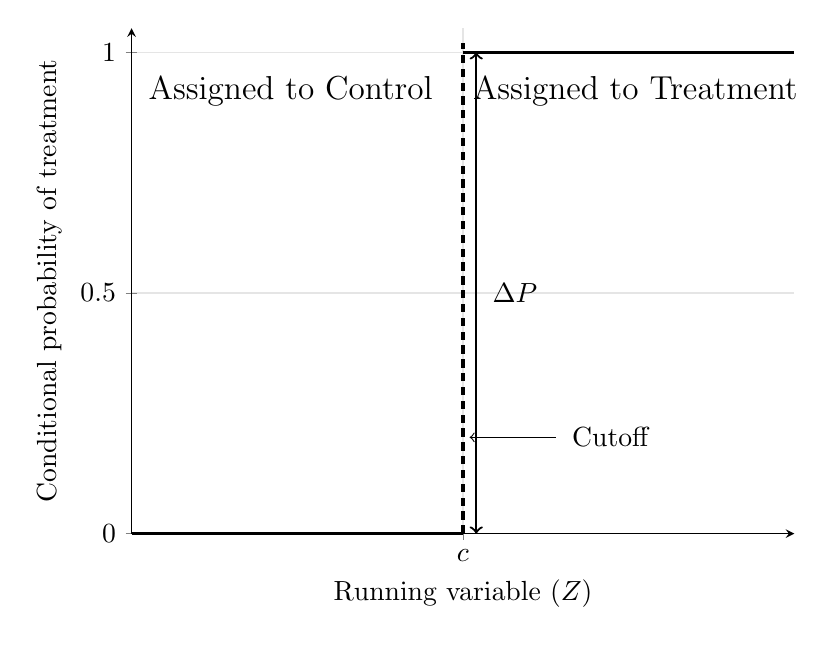
\begin{tikzpicture}
		\begin{axis}[
			width=10cm,height=8cm,
			xmin=-1, xmax=1, ymin=0, ymax=1.05,
			axis lines=left,
			grid=both, grid style={gray!20},
			xlabel={Running variable ($Z$)},
			ylabel={Conditional probability of treatment},
			xtick={0}, xticklabels={$c$},
			ytick={0,0.5,1},
			clip=false
			]
			% Sharp RD step:
			\addplot[very thick] coordinates {(-1,0) (0,0)};
			\addplot[very thick]  coordinates {(0,1) (1,1)};
			
			% Cutoff (vertical dashed line)
			\addplot[black, densely dashed, very thick] coordinates {(0,0) (0,1.02)};
			
			% Labels
			\node[black] at (axis cs:-0.52,0.92) {\large Assigned to Control};
			\node[black]  at (axis cs: 0.52,0.92) {\large Assigned to Treatment};
			
			% Arrow and text to mark "Cutoff"
			\draw[->] (axis cs:0.28,0.2) -- (axis cs:0.02,0.2);
			\node[anchor=west] at (axis cs:0.3,0.2) {Cutoff};
			
			% Bracket showing jump size (optional)
			\draw[<->, thick] (axis cs:0.04,0.0) -- (axis cs:0.04,1);
			\node[anchor=west] at (axis cs:0.06,0.50) {$\Delta P$};
		\end{axis}
	\end{tikzpicture}
\caption{Sharp regression discontinuity design: Conditional probability of treatment}
\label{Fig:SRDD}
\end{figure}

The observed outcome is given by
\begin{align*}
	Y_i=(1-D_i)\cdot Y_i(0) + D_i\cdot Y_i(1)=\begin{Bmatrix}
		Y_i(0), & Z_i < c\\
		Y_i(1), & Z_i \geq c.
	\end{Bmatrix}
\end{align*}

Thus, the causal effect that we target in SRD is
\[
\tau_{SRD}=\mathbb{E}[Y_i(1)-Y_i(0)\mid Z_i=c].
\]

Note that the treatment effect is evaluated at the cutoff, which is a single point in the support of the running variable. Hence $\tau_{\text{SRD}}$ is inherently local and need not be representative of units whose running variable lies far from $c$.
The identification of $\tau_{\text{SRD}}$ requires \emph{continuity of the potential outcome regression functions}, that is,
\[
\mathbb{E}[Y_i(0)\mid Z_i=z]\ \text{and}\ \mathbb{E}[Y_i(1)\mid Z_i=z]
\]
are continuous at $z$. Strictly speaking, it suffices that the left- and right-hand limits of $\mathbb{E}[Y_i(d)\mid Z_i=z]$ coincide at $z=c$ for $d\in\{0,1\}$.

This implies
\begin{align*}
	\mathbb{E}[Y_i(0)\mid Z_i=c]
	&= \lim_{z \uparrow c}\mathbb{E}[Y_i(0)\mid Z_i=z] \\
	&= \lim_{z \uparrow c}\mathbb{E}[Y_i(0)\mid Z_i=z, D_i=0] \\
	&= \lim_{z \uparrow c}\mathbb{E}[Y_i\mid Z_i=z],
\end{align*}
since for $z<c$ we have $D_i=0$. Similarly,
\begin{align*}
	\mathbb{E}[Y_i(1)\mid Z_i=c]
	&= \lim_{z \downarrow c}\mathbb{E}[Y_i(1)\mid Z_i=z] \\
	&= \lim_{z \downarrow c}\mathbb{E}[Y_i\mid Z_i=z],
\end{align*}
because for $z>c$ we have $D_i=1$. Therefore,
\[
\tau_{\text{SRD}}
= \lim_{z \downarrow c}\mathbb{E}[Y_i\mid Z_i=z]
- \lim_{z \uparrow c}\mathbb{E}[Y_i\mid Z_i=z],
\]
i.e., the target estimand is the jump in the conditional mean at the discontinuity point $c$. See Figure \ref{fig:SRD-muplus-muminus}.

\begin{figure}[ht]
	\centering
	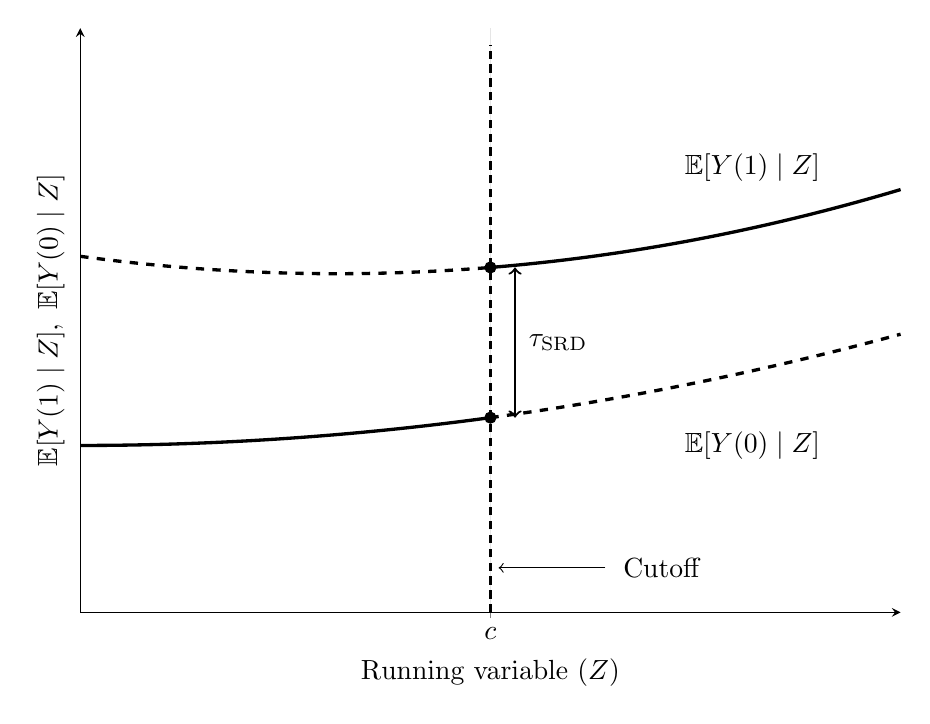
\begin{tikzpicture}
		\begin{axis}[
			width=12cm,height=9cm,
			xmin=-1, xmax=1, ymin=0, ymax=1.05,
			axis lines=left,
			grid=both, grid style={gray!20},
			xlabel={Running variable ($Z$)},
			ylabel={$\mathbb{E}[Y(1)\mid Z],\ \mathbb{E}[Y(0)\mid Z]$},
			xtick={0}, xticklabels={$c$},
			ytick=\empty,
			clip=false
			]
			
			% --- Choose smooth functions for illustration ---
			% E[Y(0)|X]: observed (solid) for X<c, counterfactual (dashed) for X>=c
			\addplot[black, very thick, domain=-1:0, samples=200] {0.35 + 0.1*x + 0.05*x^2};
			\addplot[black, very thick, dashed, domain=0:1, samples=200] {0.35 + 0.1*x + 0.05*x^2};
			
			% E[Y(1)|X]: counterfactual (dashed) for X<c, observed (solid) for X>=c
			\addplot[black, very thick, dashed, domain=-1:0, samples=200] {0.62 + 0.06*x + 0.08*x^2};
			\addplot[black, very thick, domain=0:1, samples=200] {0.62 + 0.06*x + 0.08*x^2};
			
			% --- Cutoff (vertical dashed line) ---
			\addplot[black, densely dashed, very thick] coordinates {(0,0) (0,1.02)};
			
			% --- Points at the cutoff (mu_- and mu_+) ---
			\filldraw[black] (axis cs:0,0.35) circle (2pt);  % mu_-
			\filldraw[black] (axis cs:0,0.62) circle (2pt);  % mu_+
			
			% Labels mu_- and mu_+
			% \node[anchor=east] at (axis cs:-0.02,0.35) {$\mu_-$};
			% \node[anchor=east] at (axis cs:-0.02,0.62) {$\mu_+$};
			
			% --- Jump size tau_SRD ---
			\draw[<->, thick] (axis cs:0.06,0.35) -- (axis cs:0.06,0.62);
			\node[anchor=west] at (axis cs:0.07,0.485) {$\tau_{\text{SRD}}$};
			
			% --- Arrow + label "Cutoff" ---
			\draw[->] (axis cs:0.28,0.08) -- (axis cs:0.02,0.08);
			\node[anchor=west] at (axis cs:0.30,0.08) {Cutoff};
			
			% --- Curve labels ---
			\node[black, anchor=west]  at (axis cs:0.45,0.80) {$\mathbb{E}[Y(1)\mid Z]$};
			\node[black, anchor=west] at (axis cs:0.45,0.30) {$\mathbb{E}[Y(0)\mid Z]$};
			
		\end{axis}
	\end{tikzpicture}
	\caption{RD treatment effect in a sharp RD design. Solid segments are observed on each side of $c$; dashed segments are counterfactual \cite{cattaneo2019practical}.}
	\label{fig:SRD-muplus-muminus}
\end{figure}

\subsection{Fuzzy regression discontinuity design (FRD)}

In the fuzzy case, the conditional probability of treatment has a discontinuous jump at the cutoff that is strictly between $0$ and $1$:
\begin{align*}
	\lim_{z \uparrow c} \Pr(D_i=1 \mid Z_i=z) \ne \lim_{z \downarrow c} \Pr(D_i=1 \mid Z_i=z),\\
	0 \;<\; \lim_{z \downarrow c} \Pr(D_i=1 \mid Z_i=z) \;-\; \lim_{z \uparrow c} \Pr(D_i=1 \mid Z_i=z) \;<\; 1.
\end{align*}
Thus, the probability of treatment increases discontinuously at $c$. Note that in a fuzzy RD, compliance is imperfect: some units assigned to treatment do not take it, and some units not assigned may nonetheless receive it. Figure \ref{Fig:FRDD} displays the conditional probability of treatment.

% Requires: \usepackage{tikz,pgfplots}
%           \pgfplotsset{compat=1.18}
\begin{figure}[ht]
	\centering
	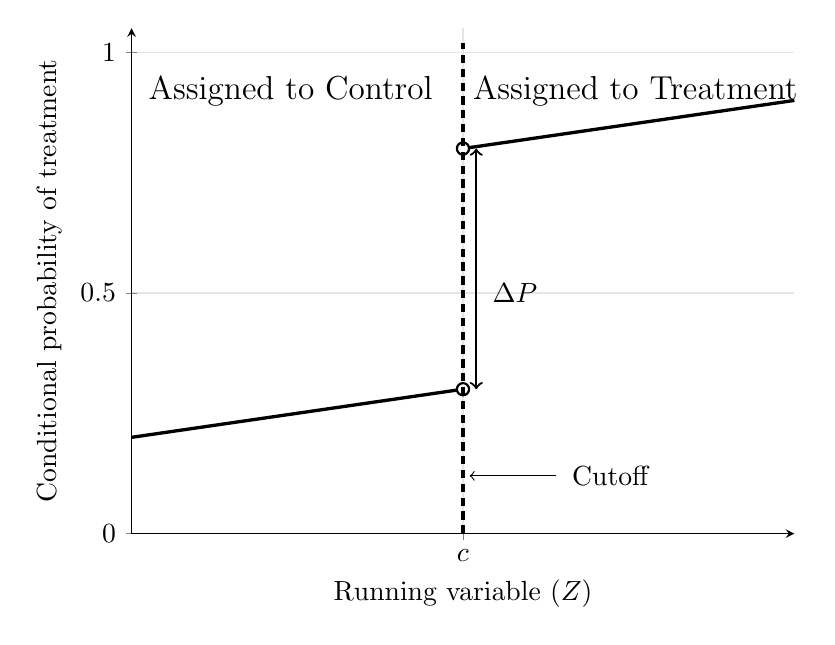
\begin{tikzpicture}
		\begin{axis}[
			width=10cm,height=8cm,
			xmin=-1, xmax=1, ymin=0, ymax=1.05,
			axis lines=left,
			grid=both, grid style={gray!20},
			xlabel={Running variable ($Z$)},
			ylabel={Conditional probability of treatment},
			xtick={0}, xticklabels={$c$},
			ytick={0,0.5,1},
			clip=false
			]
			% Fuzzy RD: probabilities below/above cutoff
			\addplot[very thick] coordinates {(-1,0.20) (0,0.30)};  % left limit p^-
			\addplot[very thick] coordinates {(0,0.80) (1,0.90)};   % right limit p^+
			
			% Open circles at the jump (left/right limits at c)
			\draw[thick, fill=white] (axis cs:0,0.30) circle (2.2pt);
			\draw[thick, fill=white] (axis cs:0,0.80) circle (2.2pt);
			
			% Cutoff (vertical dashed line)
			\addplot[black, densely dashed, very thick] coordinates {(0,0) (0,1.02)};
			
			% Labels for regions
			\node[black] at (axis cs:-0.52,0.92) {\large Assigned to Control};
			\node[black] at (axis cs: 0.52,0.92) {\large Assigned to Treatment};
			
			% Arrow and text to mark "Cutoff"
			\draw[->] (axis cs:0.28,0.12) -- (axis cs:0.02,0.12);
			\node[anchor=west] at (axis cs:0.30,0.12) {Cutoff};
			
			% Bracket showing jump size (optional)
			\draw[<->, thick] (axis cs:0.04,0.30) -- (axis cs:0.04,0.80);
			\node[anchor=west] at (axis cs:0.06,0.50) {$\Delta P$};
			
		\end{axis}
	\end{tikzpicture}
	\caption{Fuzzy regression discontinuity design: Conditional probability of treatment}
	\label{Fig:FRDD}
\end{figure}

Note that the expected value of the observed outcome given the running variable is given by
\begin{align*}
	\mathbb{E}[Y_i\mid Z_i=z]&=\mathbb{E}[Y_i(0)\mid D_i=0, Z_i=z]P(D_i=0\mid Z_i=z)\\
	&+\mathbb{E}[Y_i(1)\mid D_i=1, Z_i=z]P(D_i=1\mid Z_i=z).
\end{align*}

Thus, the observed outcome is a weighted average of potential outcomes. Figure \ref{fig:FRD-muplus-muminus} displays the treatment effect that we are targeting.

\begin{figure}[ht]
	\centering
	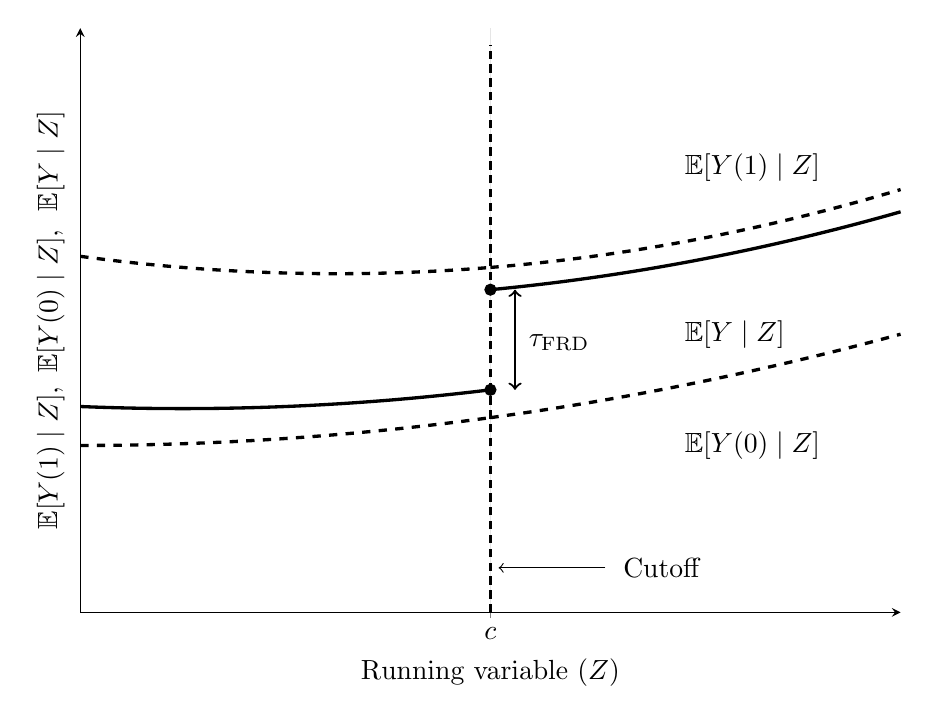
\begin{tikzpicture}
		\begin{axis}[
			width=12cm,height=9cm,
			xmin=-1, xmax=1, ymin=0, ymax=1.05,
			axis lines=left,
			grid=both, grid style={gray!20},
			xlabel={Running variable ($Z$)},
			ylabel={$\mathbb{E}[Y(1)\mid Z],\ \mathbb{E}[Y(0)\mid Z]$, \ $\mathbb{E}[Y\mid Z]$},
			xtick={0}, xticklabels={$c$},
			ytick=\empty,
			clip=false
			]
			
			% --- Choose smooth functions for illustration ---
			% E[Y(0)|X]: observed (solid) for X<c, counterfactual (dashed) for X>=c
			\addplot[black, very thick, dashed, domain=-1:0, samples=200] {0.35 + 0.1*x + 0.05*x^2};
			\addplot[black, very thick, dashed, domain=0:1, samples=200] {0.35 + 0.1*x + 0.05*x^2};
			
			% E[Y(1)|X]: counterfactual (dashed) for X<c, observed (solid) for X>=c
			\addplot[black, very thick, dashed, domain=-1:0, samples=200] {0.62 + 0.06*x + 0.08*x^2};
			\addplot[black, very thick, dashed, domain=0:1, samples=200] {0.62 + 0.06*x + 0.08*x^2};
			
			% E[Y(1)|X]: counterfactual (dashed) for X<c, observed (solid) for X>=c
			\addplot[black, very thick, domain=-1:0, samples=200] {0.4 + 0.09*x + 0.06*x^2};
			\addplot[black, very thick, domain=0:1, samples=200] {0.58 + 0.07*x + 0.07*x^2};
			
			% --- Cutoff (vertical dashed line) ---
			\addplot[black, densely dashed, very thick] coordinates {(0,0) (0,1.02)};
			
			% --- Points at the cutoff (mu_- and mu_+) ---
			\filldraw[black] (axis cs:0,0.4) circle (2pt);  % mu_-
			\filldraw[black] (axis cs:0,0.58) circle (2pt);  % mu_+
			
			% Labels mu_- and mu_+
			% \node[anchor=east] at (axis cs:-0.02,0.35) {$\mu_-$};
			% \node[anchor=east] at (axis cs:-0.02,0.62) {$\mu_+$};
			
			% --- Jump size tau_SRD ---
			\draw[<->, thick] (axis cs:0.06,0.4) -- (axis cs:0.06,0.58);
			\node[anchor=west] at (axis cs:0.07,0.485) {$\tau_{\text{FRD}}$};
			
			% --- Arrow + label "Cutoff" ---
			\draw[->] (axis cs:0.28,0.08) -- (axis cs:0.02,0.08);
			\node[anchor=west] at (axis cs:0.30,0.08) {Cutoff};
			
			% --- Curve labels ---
			\node[black, anchor=west]  at (axis cs:0.45,0.80) {$\mathbb{E}[Y(1)\mid Z]$};
			\node[black, anchor=west] at (axis cs:0.45,0.30) {$\mathbb{E}[Y(0)\mid Z]$};
			\node[black, anchor=west] at (axis cs:0.45,0.50) {$\mathbb{E}[Y\mid Z]$};
			
		\end{axis}
	\end{tikzpicture}
	\caption{RD treatment effect in a fuzzy RD design. Solid segments are observed on each side of $c$; dashed segments are counterfactual.}
	\label{fig:FRD-muplus-muminus}
\end{figure}

The target causal effect in the FRD is (see \cite{hahn2001rdd} for a proof)
\begin{align*}
\tau_{\text{FRD}}
&=
\frac{\lim_{z \downarrow c}\mathbb{E}[Y_i\mid Z_i=z]-\lim_{z \uparrow c}\mathbb{E}[Y_i\mid Z_i=z]}
{\lim_{z \downarrow c}\mathbb{E}[D_i\mid Z_i=z]-\lim_{z \uparrow c}\mathbb{E}[D_i\mid Z_i=z]}\\
&=\mathbb{E}[Y_i(1)-Y_i(0)\mid Z_i=c], \text{units are compliers}.
\end{align*}
Note that $\tau_{\text{FRD}}$ encompasses $\tau_{\text{SRD}}$ as $\lim_{z \downarrow c}\mathbb{E}[D_i\mid Z_i=z]-\lim_{z \uparrow c}\mathbb{E}[D_i\mid Z_i=z]=1$ in the SRD. In addition, $\tau_{\text{FRD}}$ has the same structure as the local average treatment effect (LATE) in the IV literature, with the instrument given by the eligibility indicator \(T_i=\mathbf{1}\{Z_i\ge c\}\). Because compliance is imperfect (some eligible units do not take treatment and some ineligible units receive it), \(D_i \neq T_i\) for some units, and the estimand pertains to \emph{compliers at the cutoff}.

Let \(D_i(z)\) denote the potential treatment status if the cutoff were \(z\) (for \(z\) in a neighborhood of \(c\)) such that $D_i(z)=1$ implies that the unit would be treated if the cutoff is $z$. The identification assumptions are: 

\textit{1. Continuity of the potential outcome regression functions}, particularly at \(c\).

\textit{2. A nontrivial first stage},
\(\lim_{z \downarrow c}\mathbb{E}[D_i\mid Z_i=z]-\lim_{z \uparrow c}\mathbb{E}[D_i\mid Z_i=z]\neq 0\),

and 

\textit{3. Monotonicity}: \(D_i(z)\) is non-increasing in \(z\) at \(z=c\).

We can classify unit types (locally around the cutoff $c$) using the potential treatment under a hypothetical cutoff $z$, $D_i(z)$ as follows:

\textit{Complier status} \[ \lim_{z\downarrow Z_i}D_i(z)=0, \ \text{and} \ \lim_{z\uparrow Z_i}D_i(z)=1, \]
 
\textit{Never-takers} \[ \lim_{z\downarrow Z_i}D_i(z)=0, \ \text{and} \ \lim_{z\uparrow Z_i}D_i(z)=0, \] 

and
 
\textit{Always-takers} \[ \lim_{z\downarrow Z_i}D_i(z)=1, \ \text{and} \ \lim_{z\uparrow Z_i}D_i(z)=1. \]

Thus, compliers are units that would be treated if the cutoff were at or below their score $Z_i$, and would not be treated if the cutoff were above $Z_i$. Never-takers and always-takers do not change treatment status regardless of the cutoff: the former are always untreated, whereas the latter are always treated. Monotonicity precludes \emph{defiers}.

See \cite{imbens2008regression} and \cite{cattaneo2019practical} for discussions of graphical and formal diagnostics of the assumptions in RD.\\

\textbf{Example: Returns to compulsory schooling \cite{chib2016bayesian}}

\cite{chib2016bayesian} propose a Bayesian inferential framework that explicitly models unit type (complier, always-taker, and never-taker), which enables implementation of a Gibbs sampler. Their empirical application is motivated by the April 1947 reform in the United Kingdom that raised the minimum school-leaving age from 14 to 15.

In the example below, we construct a simulation calibrated to their application to illustrate Bayesian inference in a fuzzy RD. In particular, we specify priors, derive the full conditional distributions, and implement a Gibbs sampler to estimate the treatment effect at the cutoff.

There are three types of individuals: compliers ($c$), never-takers ($n$), and always-takers ($a$). These imply four potential outcomes $Y_{ic}(0)$, $Y_{ic}(1)$, $Y_{in}(0)$, and $Y_{ia}(1)$. \cite{chib2016bayesian} assume
\[
Y_{ic}(0)=\beta_{0c0}+\beta_{0c1}Z_i+\mathbf{X}_i^{\top}\boldsymbol{\beta}_c+\mu_{0ci}=\mathbf{W}_{ic}^{\top}\beta_{0c}+\mu_{0ci},
\]
\[
Y_{ic}(1)=\beta_{1c0}+\beta_{1c1}Z_i+\mathbf{X}_i^{\top}\boldsymbol{\beta}_c+\mu_{1ci}=\mathbf{W}_{ic}^{\top}\beta_{1c}+\mu_{1ci},
\]
\[
Y_{in}(0)=\beta_{n0}+\mathbf{X}_i^{\top}\boldsymbol{\beta}_n+\mu_{ni}=\mathbf{W}_{in}^{\top}\beta_{0n}+\mu_{ni},
\]
and
\[
Y_{ia}(1)=\beta_{a0}+\mathbf{X}_i^{\top}\boldsymbol{\beta}_a+\mu_{ai}=\mathbf{W}_{ia}^{\top}\beta_{1a}+\mu_{ai},
\]
where $\mu_{dci}\sim t_v(0,\sigma^2_{dc})$ for $d\in\{0,1\}$, $\mu_{ni}\sim t_v(0,\sigma^2_{0n})$, and $\mu_{ai}\sim t_v(0,\sigma^2_{1a})$; here $t_v$ denotes the Student-$t$ distribution with $v$ degrees of freedom. The running variable is centered at the cutoff, so $Z_i=0$ at the threshold, and the FRD treatment effect is
\[
\tau_{\text{FRD}}=\beta_{1c0}-\beta_{0c0}.
\]

There are four cells in this setting, defined by policy epochs $\mathbbm{1}(Z_i < 0)$ and $\mathbbm{1}(Z_i \geq 0)$, and treatment values $D_i = 0$ and $D_i = 1$. Table \ref{tab:appCJ} shows the case where, in the cell without treatment under the old policy ($K_{00}$), there are compliers and never-takers, while in the cell with treatment under the new policy ($K_{11}$), there are compliers and always-takers.

\begin{table}[ht]
	\centering
	\caption{Distribution of subject type by observed policy regime and treatment}\label{tab:appCJ}
	\begin{tabular}{lcc}
		\hline
		& \multicolumn{2}{c}{\textbf{Treatment}} \\ 
		\cline{2-3}
		\textbf{Policy indicator} & $D_i = 0$ & $D_i = 1$ \\ 
		\hline
		$\mathbbm{1}(Z_i < 0)$ (old policy) & c, n & a \\
		$\mathbbm{1}(Z_i \geq 0)$ (new policy) & n & c, a \\
		\hline
	\end{tabular}
\end{table}

The four cells by policy and treatment status are:
\[
K_{00} = \{c, n\}, \quad K_{10} = \{n\}, \quad K_{01} = \{a\}, \quad K_{11} = \{c, a\},
\]
and the two cells by treatment status are:
\[
K_0 = \{c, n\}, \quad K_1 = \{c, a\}.
\]

Under a Bayesian framework, posterior simulation simplifies because we sample each unit’s latent type $C_i \in \{c, n, a\}$. This contrasts with the Frequentist literature, where types are not modeled explicitly. Thus, the Bayesian approach requires setting assumptions about the types (see \cite{chib2016bayesian} for details); for instance, types may be distributed smoothly around the cutoff with unknown distributions. In addition, given monotonicity, there are models for four potential outcomes. This differs from the Frequentist literature, which considers only two potential outcomes, given the binary treatment, and a model for the treatment.

Note that if we observe $Z_i < 0$ and $D_i = 0$, only compliers and never-takers are possible. Then,
\[
P(C_i = c \mid Y_i, D_i = 0, \boldsymbol{\theta})
= \frac{\eta_{c} \, t_v\!\big(Y_i \mid \mathbf{W}_{ic}^{\top} \boldsymbol{\beta}_{0c}, \sigma^2_{0c} \big)}
{\eta_{c} \, t_v\!\big(Y_i \mid \mathbf{W}_{ic}^{\top} \boldsymbol{\beta}_{0c}, \sigma^2_{0c} \big) +
	\eta_{n} \, t_v\!\big(Y_i \mid \mathbf{W}_{in}^{\top} \boldsymbol{\beta}_{0n}, \sigma^2_{0n} \big)}, i \in K_{00}
\]
where $\boldsymbol{\theta}$ denotes the set of model parameters, and $\eta_{c}$ and $\eta_{n}$ are the current mixture weights for a complier and a never-taker, respectively.

Conversely, if $Z_i \geq 0$ and $D_i = 1$, only compliers and always-takers are possible:
\[
P(C_i = c \mid Y_i, D_i = 1, \boldsymbol{\theta})
= \frac{\eta_{c} \, t_v\!\big(Y_i \mid \mathbf{W}_{ic}^{\top} \boldsymbol{\beta}_{1c}, \sigma^2_{1c} \big)}
{\eta_{c} \, t_v\!\big(Y_i \mid \mathbf{W}_{ic}^{\top} \boldsymbol{\beta}_{1c}, \sigma^2_{1c} \big) +
	\eta_{a} \, t_v\!\big(Y_i \mid \mathbf{W}_{ia}^{\top} \boldsymbol{\beta}_{1a}, \sigma^2_{1a} \big)}, i \in K_{11}
\]
where $\eta_{a}$ is the mixture weight for an always-taker.

Following \cite{chib2016bayesian}, we assume a Dirichlet prior for the mixing probabilities ($\eta_c, \eta_n,\eta_a$) with hyperparameters $\alpha_{0k}$, $k \in \{c, n, a\}$. The posterior distribution is then Dirichlet with parameters $\alpha_{0k} + \sum_{i=1}^N \mathbbm{1}(C_i = k)$.

In addition, \cite{chib2016bayesian} use the normal--gamma mixture representation of the Student-$t$ distribution, where the mixing parameter satisfies $\lambda_i \sim G(v/2, v/2)$. Consequently, the posterior distribution of $\lambda_i$ is gamma with parameters $(v+1)/2$ and $(v + \sigma_{dk}^{-2}(y_i - \mathbf{W}_{ik}^{\top} \boldsymbol{\beta}_{dk})^2) / 2$.

The prior distribution for the location parameters $\boldsymbol{\beta}_{dk}$ is independent normal with mean $\boldsymbol{\beta}_{dk,0}$ and variance matrix $\mathbf{B}_{dk,0}$. The posterior distribution of $\boldsymbol{\beta}_{dk}$ is normal with mean
\[
\boldsymbol{\beta}_{dk,n} = \mathbf{B}_{dk,n} \left( \mathbf{B}_{dk,0}^{-1} \boldsymbol{\beta}_{dk,0} + \sigma_{dk}^{-2} \sum_{i \in I_{dk}} \lambda_i \mathbf{W}_{ik} Y_i \right),
\]
and covariance matrix
\[
\mathbf{B}_{dk,n} = \left( \mathbf{B}_{dk,0}^{-1} + \sigma_{dk}^{-2} \sum_{i \in I_{dk}} \lambda_i \mathbf{W}_{ik} \mathbf{W}_{ik}^{\top} \right)^{-1},
\]
where $I_{dk} = \{i : D_i = d, C_i = k\}$ is the set of indices for observations by treatment status and unit type. Note that there are only four possible combinations determined by policy and treatment status, namely, $I_{0c}$, $I_{1c}$, $I_{0n}$ and $I_{1a}$.

Finally, assuming that the prior distributions of the variances are independent inverse-gamma, $\sigma_{dk}^2 \sim IG(\alpha_{dk,0}/2, \delta_{dk,0}/2)$, the posterior distributions are also inverse-gamma, $\sigma_{dk}^2 \sim IG(\alpha_{dk,n}/2, \delta_{dk,n}/2)$, where
\[
\alpha_{dk,n} = \alpha_{dk,0} + N_{dk},
\]
and
\[
\delta_{dk,n} = \delta_{dk,0} + \sum_{i \in I_{dk}} \lambda_i \left(Y_i - \mathbf{w}_{ik}^{\top} \boldsymbol{\beta}_{dk} \right)^2.
\]
Here, $N_{dk}$ denotes the number of elements (cardinality) of $I_{dk}$.

The following code performs a simulation assuming that $Z_i$ follows a discrete uniform distribution from $-24$ to $24$, where the policy indicator equals one if $Z_i \geq 0$. Next, $X_i$ follows a discrete uniform distribution between $85$ and $95$. We set $\boldsymbol{\beta}_{0c} = [4.50 \ -0.20 \ 0.03]^{\top}$ and $\boldsymbol{\beta}_{1c} = [5.50 \ 0.40 \ 0.03]^{\top}$, so that the treatment effect is $1$. In addition, $\boldsymbol{\beta}_{0n} = [6.80 \ -0.02]^{\top}$ and $\boldsymbol{\beta}_{1a} = [5.50 \ -0.04]^{\top}$, with $\sigma_{0c}^2 = \sigma_{1c}^2 = 0.10$, $\sigma_{0n}^2 = 0.15$, and $\sigma_{1a}^2 = 0.20$. The type probabilities are $\eta_{c} = 0.70$, $\eta_{n} = 0.15$, and $\eta_{a} = 0.15$. We set the sample size to $3{,}000$ and $v = 5$. In addition, we set non-informative priors, a burn-in of 1,000, and 5,000 MCMC iterations. The following code illustrates the implementation, and Figure \ref{fig12_FRD} presents the posterior distribution of the LATE. The 95\% credible interval encompasses the population value, and the posterior mean lies close to this value.

\begin{tcolorbox}[enhanced,width=4.67in,center upper,
	fontupper=\large\bfseries,drop shadow southwest,sharp corners]
	\textit{R code. Simulation: Fuzzy regression discontinuity design}
	\begin{VF}
		\begin{lstlisting}[language=R]		
rm(list = ls()); set.seed(10101)
# Simulation setup
N <- 3000
Zi <- sample(seq(-24, 24, 1), N, replace = TRUE) # Running var
Z <- Zi - mean(Zi)
T <- as.integer(Z >= 0)                          # Policy (0/1)
X <- sample(seq(85, 95, 1), N, replace = TRUE)   # Regressor
Wc <- cbind(1, Z, X)                             # Compliers
W  <- cbind(1, X)                                # No compliers

B0c <- c(4.5, -0.2, 0.03); B1c <- c(5.5, 0.4,  0.03)
B0n <- c(6.8,  -0.02); B1a <- c(5.5,  -0.04)
s2c <- 0.1; s2n <- 0.15; s2a <- 0.2
Etac <- 0.7; Etan <- 0.15; Etaa <- 0.15
v <- 5
# Potential outcomes (Student-t noise scaled to match variances)
mu0c <- sqrt(s2c) * rt(N, v);  Y0c <- as.numeric(Wc %*% B0c + mu0c)
mu1c <- sqrt(s2c) * rt(N, v);  Y1c <- as.numeric(Wc %*% B1c + mu1c)
mu0n <- sqrt(s2n) * rt(N, v);  Y0n <- as.numeric(W  %*% B0n + mu0n)
mu1a <- sqrt(s2a) * rt(N, v);  Y1a <- as.numeric(W  %*% B1a + mu1a)
# Latent types: first n, then a, remaining are c
id    <- seq_len(N)
n_n   <- as.integer(round(Etan * N))
n_a   <- as.integer(round(Etaa * N))
id0n  <- sample(id, n_n, replace = FALSE)     # never-takers
id_rem <- setdiff(id, id0n)
id1a  <- sample(id_rem, n_a, replace = FALSE) # always-takers
idc   <- setdiff(id, c(id0n, id1a))           # compliers
type <- rep(NA_character_, N)
type[id0n] <- "n"
type[id1a] <- "a"
type[idc]  <- "c"
# Realized treatment under monotonicity:
# n -> D=0, a -> D=1, c -> D=T
D <- integer(N)
D[type == "n"] <- 0; D[type == "a"] <- 1
D[type == "c"] <- T[type == "c"]

# 2x2 table of D vs T
tab_DT <- table(T = factor(T, levels = 0:1), D = factor(D, levels = 0:1))
print(tab_DT)
		\end{lstlisting}
	\end{VF}
\end{tcolorbox}  

\begin{tcolorbox}[enhanced,width=4.67in,center upper,
	fontupper=\large\bfseries,drop shadow southwest,sharp corners]
	\textit{R code. Simulation: Fuzzy regression discontinuity design}
	\begin{VF}
		\begin{lstlisting}[language=R]	
Y <- ifelse(type == "n", Y0n, ifelse(type == "a", Y1a, ifelse(D == 0, Y0c, Y1c)))
## Gibbs sampler ##
I00 <- which(T == 0 & D == 0); I11 <- which(T == 1 & D == 1)
I01 <- which(T == 0 & D == 1); I10 <- which(T == 1 & D == 0)
# Hyperparameters
a0c <- 1; a0n <- 1; a0a <- 1 # Hyperpar Dirichlet
v <- 5 # Student-t
a0 <- 0.01; d0 <- 0.01 # Inv-Gamma
# Prob complier | D=0
dens_t_locscale <- function(y, mu, sig2, v) {
	z <- (y - mu) / sqrt(sig2); dt(z, df = v) / sqrt(sig2)
}
Pc0 <- function(b0c, sigma20c, etac, b0n, sigma20n, etan, i){
	p0c <- etac * dens_t_locscale(Y[i], mu = sum(Wc[i,]*b0c), sig2 = sigma20c, v = v)
	p0n <- etan * dens_t_locscale(Y[i], mu = sum(W[i, ]*b0n), sig2 = sigma20n, v = v)
	pc0 <- p0c / (p0c + p0n + 1e-12)
	return(pc0)
}
Pc1 <- function(b1c, sigma21c, etac, b1a, sigma21a, etaa, i){
	p1c <- etac * dens_t_locscale(Y[i], mu = sum(Wc[i,]*b1c), sig2 = sigma21c, v = v)
	p1a <- etaa * dens_t_locscale(Y[i], mu = sum(W[i, ]*b1a), sig2 = sigma21a, v = v)
	pc1 <- p1c / (p1c + p1a + 1e-12)
	return(pc1)
}
rtype <- function(alphas){
	types <- MCMCpack::rdirichlet(1, alphas)
	return(types)
}
PostLambda_i <- function(sig2, Beta, yi, hi, v){
	shape <- (v + 1)/2
	rate  <- (v + (yi - sum(hi * Beta))^2 / sig2)/2
	rgamma(1, shape = shape, rate = rate)
}
PostBeta <- function(sig2, lambda, y, H){
	k <- dim(H)[2]; B0i <- solve(1000*diag(k))
	b0 <- rep(0, k)
	Bn <- solve(B0i + sig2^(-1)*t(H)%*%diag(lambda)%*%H)
	bn <- Bn%*%(B0i%*%b0 + sig2^(-1)*t(H)%*%diag(lambda)%*%y)
	Beta <- MASS::mvrnorm(1, bn, Bn)
	return(Beta)
}
PostSig2 <- function(Beta, lambda, y, H){
	Ndk <- length(y); an <- a0 + Ndk 
	dn <- d0 + t(y - H%*%Beta)%*%diag(lambda)%*%(y - H%*%Beta)
	sig2 <- invgamma::rinvgamma(1, shape = an/2, rate = dn/2)
	return(sig2)
}
\end{lstlisting}
	\end{VF}
\end{tcolorbox}  

\begin{tcolorbox}[enhanced,width=4.67in,center upper,
	fontupper=\large\bfseries,drop shadow southwest,sharp corners]
	\textit{R code. Simulation: Fuzzy regression discontinuity design}
	\begin{VF}
		\begin{lstlisting}[language=R]	
# MCMC parameter
burnin <- 1000; S <- 5000; tot <- S + burnin 
ETAs <- matrix(NA, tot, 3)
BETAS0C <- matrix(NA, tot, 3); BETAS1C <- matrix(NA, tot, 3)
BETASA <- matrix(NA, tot, 2); BETASN <- matrix(NA, tot, 2)
SIGMAS <- matrix(NA, tot, 4)
b0c <- rep(0, 3); b1c <- rep(0, 3); b1a <- rep(0, 2); b0n <- rep(0, 2)
sigma21c <- 0.1; sigma20c <- 0.1; sigma20n <- 0.1; sigma21a <- 0.1
EtacNew <- 0.5; EtanNew <- 0.25; EtaaNew <- 0.25
pb <- winProgressBar(title = "progress bar", min = 0, max = tot, width = 300)
for(s in 1:tot){
	ProbC0 <- sapply(I00, function(i)Pc0(b0c, sigma20c, EtacNew, b0n, sigma20n, EtanNew, i = i))
	ProbC1 <- sapply(I11, function(i)Pc1(b1c, sigma21c, EtacNew, b1a, sigma21a, EtaaNew, i = i))
	Typec0 <- sapply(ProbC0, function(p) {sample(c("c", "n"), 1, prob = c(p, 1-p))})
	Typec1 <- sapply(ProbC1, function(p) {sample(c("c", "a"), 1, prob = c(p, 1-p))})
	typeNew <- rep(NA_character_, N)
	typeNew[I10] <- "n"; typeNew[I01] <- "a"
	typeNew[I00]  <- Typec0; typeNew[I11]  <- Typec1
	Nc <- sum(typeNew == "c"); Na <- sum(typeNew == "a")
	Nn <- sum(typeNew == "n");
	anc <- a0c + Nc; ann <- a0n + Nn; ana <- a0a + Na
	alphas <- c(anc, ann, ana)
	EtasNew <- rtype(alphas = alphas)
	EtacNew <- EtasNew[1]; EtanNew <- EtasNew[2]
	EtaaNew <- EtasNew[3]
	ETAs[s, ] <- EtasNew; Lambda <- numeric(N)
	idx_n <- which(typeNew == "n")
	idx_a <- which(typeNew == "a")
	idx_c0 <- which(typeNew == "c" & D == 0); idx_c1 <- which(typeNew == "c" & D == 1)
	Lambda[idx_n]  <- sapply(idx_n,  function(i) PostLambda_i(sigma20n, b0n, Y[i],  W[i, ], v))
	Lambda[idx_a]  <- sapply(idx_a,  function(i) PostLambda_i(sigma21a, b1a, Y[i],  W[i, ], v))
	Lambda[idx_c0] <- sapply(idx_c0, function(i) PostLambda_i(sigma20c, b0c, Y[i], Wc[i, ], v))
	Lambda[idx_c1] <- sapply(idx_c1, function(i) PostLambda_i(sigma21c, b1c, Y[i], Wc[i, ], v))
	b1a <- PostBeta(sig2 = sigma21a, lambda = Lambda[idx_a], y = Y[idx_a], H = W[idx_a,])
	b0n <- PostBeta(sig2 = sigma20n, lambda = Lambda[idx_n], y = Y[idx_n], H = W[idx_n,])
	b0c <- PostBeta(sig2 = sigma20c, lambda = Lambda[idx_c0], y = Y[idx_c0], H = Wc[idx_c0,])
	b1c <- PostBeta(sig2 = sigma21c, lambda = Lambda[idx_c1], y = Y[idx_c1], H = Wc[idx_c1,])
	BETASA[s, ] <- b1a; BETASN[s, ] <- b0n
	BETAS0C[s, ] <- b0c; BETAS1C[s, ] <- b1c 
\end{lstlisting}
	\end{VF}
\end{tcolorbox}  

\begin{tcolorbox}[enhanced,width=4.67in,center upper,
	fontupper=\large\bfseries,drop shadow southwest,sharp corners]
	\textit{R code. Simulation: Fuzzy regression discontinuity design}
	\begin{VF}
		\begin{lstlisting}[language=R]	
	sigma21a <- PostSig2(Beta = b1a, lambda = Lambda[idx_a], y = Y[idx_a], H = W[idx_a,])
	sigma20n <- PostSig2(Beta = b0n, lambda = Lambda[idx_n], y = Y[idx_n], H = W[idx_n,])
	sigma20c <- PostSig2(Beta = b0c, lambda = Lambda[idx_c0], y = Y[idx_c0], H = Wc[idx_c0,])
	sigma21c <- PostSig2(Beta = b1c, lambda = Lambda[idx_c1], y = Y[idx_c1], H = Wc[idx_c1,])
	SIGMAS[s, ] <- c(sigma21a, sigma20n, sigma20c, sigma21c)
	setWinProgressBar(pb, s, title=paste( round(s/tot*100, 0),"% done"))
}
close(pb)
keep <- seq((burnin+1), tot)
LATE <- coda::mcmc(BETAS1C[keep, 1] - BETAS0C[keep, 1])
# Extract samples as numeric
late_draws <- as.numeric(LATE)
# Posterior mean and 95% CI
LATEmean <- mean(late_draws)
LATEci   <- quantile(late_draws, c(0.025, 0.975))
# Plot posterior density
df <- data.frame(LATE = late_draws)

ggplot(df, aes(x = LATE)) + geom_density(fill = "skyblue", alpha = 0.5, color = "blue") + geom_vline(xintercept = LATEmean, color = "red", linetype = "dashed", linewidth = 1) + geom_vline(xintercept = LATEci, color = "black", linetype = "dotted", linewidth = 1) + labs(title = "Posterior distribution of LATE",
subtitle = paste0("Mean = ", round(LATEmean,3), " | 95% CI = [", round(LATEci[1],3), ", ", round(LATEci[2],3), "]"), x = "LATE", y = "Density") +
theme_bw(base_size = 14)
		\end{lstlisting}
	\end{VF}
\end{tcolorbox}  

\begin{figure}[h!]
	\includegraphics[width=340pt, height=200pt]{Chapters/chapter12/figures/FigFRD.png}
	\caption[List of figure caption goes here]{Posterior distribution of LATE: Simulation of fuzzy regression discontinuity design}\label{fig12_FRD}
\end{figure}


A difference in this example is that, unlike most of the Frequentist literature, the entire dataset on the forcing variable is used. \cite{chib2023nonparametric} propose a non-parametric Bayesian framework that emphasizes the data near the cutoff using a \textit{soft-window} approach. Other Bayesian approaches to inference in RD include \cite{branson2019nonparametric}, who use Gaussian process regression to model the conditional expectation function, and \cite{rischard2020bayesian}, who develop a non-parametric Bayesian framework for spatial RD.

\section{Sample selection}\label{sec12_8}

In Figure \ref{DAG3} in Section \ref{chap12_3}, we depict a situation of collider bias that induces selection bias. Specifically, conditioning on a particular subset of the population ($D_i=1$), where $D_i$ is influenced by both the treatment and confounders, opens a back-door path and creates a spurious association between their causes. Placing this situation within the well-known sample selection framework \cite{heckman1979sample}, the observed outcome can be represented as
\begin{align*}
	Y_i = \begin{cases}
		Y_i(1) & \text{if } D_i=1, \\
		\text{NA} & \text{if } D_i=0,
	\end{cases}
\end{align*}
that is, we only observe $Y_i = Y_i(1)$ for $i=1,2,\dots,N$, while $Y_i(0)$ remains unobserved (``missing'').

In this setting, inference can be performed based on the likelihood of the observed outcomes together with the \textit{selection (missingness) mechanism} $(Y_i(1),D_i)$, integrating out the unobserved $Y_i(0)$ from the joint distribution of $\{Y_i(1),Y_i(0),D_i\}$. However, one must consider whether the missingness mechanism is \textit{ignorable} or not. According to \cite{little2019statistical}, the missingness mechanism is ignorable in Bayesian inference if the following two conditions hold:  
i) the likelihood can be factorized as
\[
p(\boldsymbol{\theta},\boldsymbol{\gamma}\mid y_i, d_i) 
= p(\boldsymbol{\theta}\mid y_i)\, p(y_i,d_i \mid \boldsymbol{\gamma}),
\] 
and  
ii) the parameters $\boldsymbol{\theta}$ and $\boldsymbol{\gamma}$ are \emph{a priori} independent,
\[
\pi(\boldsymbol{\theta},\boldsymbol{\gamma}) 
= \pi(\boldsymbol{\theta})\,\pi(\boldsymbol{\gamma}).
\]

Under these conditions, posterior inference can be based on
\[
\pi(\boldsymbol{\theta}\mid \mathbf{y}) 
\propto \pi(\boldsymbol{\theta})\, p(\mathbf{y} \mid \boldsymbol{\theta}).
\]
Thus, if the missingness mechanism is Missing At Random (MAR) and the parameters are \emph{a priori} independent, the missingness mechanism is ignorable for Bayesian inference (see Chapter~6 of \cite{little2019statistical}).

In contrast, when the missingness mechanism is non-ignorable (i.e., Not Missing At Random, NMAR), the probability of observing $Y_i$ depends on the unobserved values themselves. In this case, Bayesian inference must be performed using the full joint likelihood,
\[
p(y_i, d_i \mid \boldsymbol{\theta},\boldsymbol{\gamma}),
\]
which requires specifying and estimating both the outcome model and the selection model simultaneously (see Chapter~15 of \cite{little2019statistical}). In particular, the classical sample selection model of \cite{heckman1979sample} establishes,
\begin{align*}
	Y_i = \begin{cases}
		\mathbf{X}_i^{\top}\boldsymbol{\beta}+\mu_i & \text{if } D_i=1, \\
		\text{NA} & \text{if } D_i=0,
	\end{cases}
\end{align*}

\begin{align*}
	D_i = \begin{cases}
		1 & \text{if } D_i^* = \mathbf{Z}_i^{\top}\boldsymbol{\gamma}+\nu_i > 0, \\
		0 & \text{if } D_i^* = \mathbf{Z}_i^{\top}\boldsymbol{\gamma}+\nu_i \leq 0,
	\end{cases}
\end{align*}

where
\begin{align}
	\begin{bmatrix}
		\mu_i \\[6pt]
		\nu_i
	\end{bmatrix}
	\sim N\!\left(
	\begin{bmatrix}
		0 \\ 0
	\end{bmatrix},
	\begin{bmatrix}
		\sigma^2_{\mu} & \sigma_{\mu\nu} \\
		\sigma_{\mu\nu} & 1
	\end{bmatrix}\right).
\end{align}
The restriction $\operatorname{Var}(\nu_i)=1$ is imposed for identification. 
Without this normalization, the latent index $D_i^*=\mathbf{Z}_i^{\top}\boldsymbol{\gamma}+\nu_i$ is only identified up to scale, since
\[
P(D_i=1) = P(\mathbf{Z}_i^{\top}\boldsymbol{\gamma}+\nu_i > 0) 
= P\!\left(\frac{\nu_i}{c} > -\frac{\mathbf{Z}_i^{\top}\boldsymbol{\gamma}}{c}\right),
\quad \forall\, c>0.
\]
Thus, setting $\sigma^2_{\nu}=1$ yields point identification of the parameters.

Note that since \(D_i=1 \iff \nu_i>-\mathbf Z_i^\top\boldsymbol\gamma\),
\[
\mathbb E[\mu_i\mid D_i=1,\mathbf Z_i]
=\mathbb E\!\big[\mathbb E(\mu_i\mid \nu_i)\,\big|\,\nu_i>-\mathbf Z_i^\top\boldsymbol\gamma\big]
=\sigma_{\mu\nu}\,\mathbb E\!\big[\nu_i\mid \nu_i>-\mathbf Z_i^\top\boldsymbol\gamma\big].
\] This is because $\mu_i\mid \nu_i\sim N(\sigma_{\mu\nu}\nu_i, \sigma^2_{\mu}-\sigma_{\mu\nu}^2)$.

If \(\nu\sim\mathcal N(0,1)\), then for \(a=\mathbf Z_i^\top\boldsymbol\gamma\),
\[
\mathbb E[\nu\mid \nu>-a]=\frac{\phi(a)}{\Phi(a)}\equiv \lambda(a),
\]
where \(\phi\) and \(\Phi\) are the standard normal pdf and cdf. Hence
\[
\mathbb E[\mu_i\mid D_i=1,\mathbf Z_i]=\sigma_{\mu\nu}\,\lambda(\mathbf Z_i^\top\boldsymbol\gamma)
	=\rho\,\sigma_\mu\,\lambda(\mathbf Z_i^\top\boldsymbol\gamma),
\]
where $\rho=\sigma_{\mu\nu}/\sigma_{\mu}$.

Then, 
\begin{align*}
	\mathbb E[Y_i\mid D_i=1,\mathbf X_i,\mathbf Z_i]
	&=\mathbf X_i^\top \boldsymbol\beta+\mathbb E[\mu_i\mid D_i=1,\mathbf Z_i]\\
	&=\mathbf X_i^\top \boldsymbol\beta + \sigma_{\mu\nu}\,\lambda(\mathbf Z_i^\top\boldsymbol\gamma)\\
	&=\mathbf X_i^\top \boldsymbol\beta + \rho\,\sigma_\mu\,\lambda(\mathbf Z_i^\top\boldsymbol\gamma).
\end{align*}

This is the Heckman selection-bias correction: the inverse Mills ratio \(\lambda(\mathbf Z_i^\top\boldsymbol\gamma)\) enters as an additional regressor in the selected sample.
Point identification can be achieved through functional form (since the inverse Mills ratio is non-linear) together with the normality assumption. This implies that, in principle, one may have $\mathbf{X}_i=\mathbf{Z}_i$. However, such identification is weak, and it is preferable to include at least one variable in $\mathbf{Z}_i$ that is excluded from $\mathbf{X}_i$, i.e., $\mathbf{X}_i\neq\mathbf{Z}_i$, as this strengthens identification and also improves the precision of inference.

To perform Bayesian inference in this model, we use the augmented likelihood. Thus,
\begin{align*}
	\pi(\boldsymbol{\delta},\sigma^2_{\mu},\sigma_{\mu\nu},D_i^*\mid \mathbf{y},\mathbf{d}) 
	& \propto \prod_{i\in I_{0}} \pi(D_i^*\mid \boldsymbol{\delta},\sigma^2_{\mu},\sigma_{\mu\nu}) 
	\, \mathbbm{1}(d_i=0)\, \mathbbm{1}(D_i^*\leq 0) \\
	& \quad \times \prod_{i\in I_{1}} p(y_i,D_i^*\mid \boldsymbol{\delta},\sigma^2_{\mu},\sigma_{\mu\nu}) 
	\, \mathbbm{1}(d_i=1)\, \mathbbm{1}(D_i^*> 0) \\
	& \quad \times \pi(\boldsymbol{\delta},\sigma^2_{\mu},\sigma_{\mu\nu}),
\end{align*}
where $\boldsymbol{\delta}=[\boldsymbol{\beta}^{\top} \ \boldsymbol{\gamma}^{\top}]^{\top}$, 
$I_0=\{i : d_i=0\}$ and $I_1=\{i : d_i=1\}$.

Following Chapter~11 in \cite{greenberg2012introduction}, we set
\[
\boldsymbol{\eta}_i=
\begin{cases}
	[0, \, D_i^*]^{\top}, & i\in I_0,\\
	[y_i, \, D_i^*]^{\top}, & i\in I_1,
\end{cases}
\qquad
\mathbf{W}_i=\begin{bmatrix}
	\mathbf{X}_i^{\top} & \mathbf{0}\\
	\mathbf{0} & \mathbf{Z}_i^{\top}
\end{bmatrix}, 
\qquad
\mathbf{J}=\begin{bmatrix}
	0 & 0\\
	0 & 1
\end{bmatrix}.
\]

Assuming $\pi(\boldsymbol{\delta}) \sim N(\boldsymbol{\delta}_0,\mathbf{D}_0)$, the conditional posterior distribution of $\boldsymbol{\delta}$ is normal with mean
\[
\boldsymbol{\delta}_n=\mathbf{D}_n\left[\sum_{i\in I_0}\mathbf{W}_i^{\top}\mathbf{J}\boldsymbol{\eta}_i
+\sum_{i\in I_1}\mathbf{W}_i^{\top}\boldsymbol{\Sigma}^{-1}\boldsymbol{\eta}_i
+\mathbf{D}_0^{-1}\boldsymbol{\delta}_0\right],
\]
and variance matrix
\[
\mathbf{D}_n=\left[\sum_{i\in I_0}\mathbf{W}_i^{\top}\mathbf{J}\mathbf{W}_i
+\sum_{i\in I_1}\mathbf{W}_i^{\top}\boldsymbol{\Sigma}^{-1}\mathbf{W}_i
+\mathbf{D}_0^{-1}\right]^{-1},
\] 
where 
\[
\boldsymbol{\Sigma}=\begin{bmatrix}
	\sigma^2_{\mu} & \sigma_{\mu\nu} \\[6pt]
	\sigma_{\mu\nu} & 1
\end{bmatrix}.
\]

Let $\omega=\sigma^2_{\mu}-\sigma^2_{\mu\nu}$ denote the conditional variance of $\mu_i \mid \nu_i$. 
Assuming $\omega^{-1}\sim G(\alpha_0/2,\delta_0/2)$ and noting that
\[
p(y_i,D_i^*\mid \boldsymbol{\delta},\omega,\sigma_{\mu\nu})
= p(y_i\mid D_i^*, \boldsymbol{\delta},\omega,\sigma_{\mu\nu})
\times p(D_i^*\mid \boldsymbol{\delta},\omega,\sigma_{\mu\nu}),
\]
the conditional posterior distribution of $\omega^{-1}$ is Gamma,
\[
\omega^{-1}\mid \boldsymbol{\delta},\sigma_{\mu\nu}, \mathbf{y},\mathbf{d} \sim G(\alpha_n/2,\delta_n/2),
\]
with
\[
\alpha_n=\alpha_0+N_1,
\qquad
\delta_n=\delta_0+\sum_{i\in I_1}\Big[y_i-\mathbf{X}_i^{\top}\boldsymbol{\beta}
-\sigma_{\mu\nu}(D_i^*-\mathbf{Z}_i^{\top}\boldsymbol{\gamma})\Big]^2,
\]
where $N_1$ is the number of observations with $D_i=1$.

In addition, assuming $\sigma_{\mu\nu}\sim N(s_0,S_0)$, the conditional posterior distribution is normal with mean
\[
s_n=S_n\left(\omega^{-1}\sum_{i=1}^N(D_i^*-\mathbf{Z}_i^{\top}\boldsymbol{\gamma})(y_i-\mathbf{X}_i^{\top}\boldsymbol{\beta})
+S_0^{-1}s_0\right),
\]
and variance
\[
S_n=\left[\omega^{-1}\sum_{i=1}^N(D_i^*-\mathbf{Z}_i^{\top}\boldsymbol{\gamma})^2+S_0^{-1}\right]^{-1}.
\]

Finally, since
\[
p(y_i,D_i^*\mid \boldsymbol{\delta},\omega,\sigma_{\mu\nu})
= p(D_i^*\mid y_i, \boldsymbol{\delta},\omega,\sigma_{\mu\nu})
\times p(y_i\mid \boldsymbol{\delta},\omega,\sigma_{\mu\nu}),
\]
the conditional posterior distribution of $D_i^*$ is
\[
D_i^* \sim 
\begin{cases}
	TN_{(-\infty,0]}(\mathbf{Z}_i^{\top}\boldsymbol{\gamma},\,1), & i\in I_0,\\[6pt]
	TN_{(0,\infty)}\!\left(\mathbf{Z}_i^{\top}\boldsymbol{\gamma}
	+\dfrac{\sigma_{\mu\nu}}{\sigma_{\mu\nu}^2+\omega}\,(y_i-\mathbf{X}_i^{\top}\boldsymbol{\beta}),\,
	\dfrac{\omega}{\sigma_{\mu\nu}^2+\omega}\right), & i\in I_1,
\end{cases}
\]
where $TN_{A}(\mu,\sigma^2)$ denotes a normal distribution with mean $\mu$ and variance $\sigma^2$, truncated to the set $A$.\\

\textbf{Example: Simulation of the sample selection model}
We simulate the model 
\[
Y_i = 12 + X_{i1} + X_{i2} + \mu_i,
\]
where $X_{i1}\sim N(0,4)$, $X_{i2}\sim \text{Bin}(1,0.5)$, and $\mu_i\sim N(0,1.2)$ for $i=1,2,\dots,1000$.  
In addition, 
\[
D_i^* = 1 + Z_{i1} - X_{i2} + \nu_i,
\]
where $Z_{i1}\sim N(0,4)$.

The covariance between $\mu_i$ and $\nu_i$ is set to $0.6$.

The hyperparameters are $\boldsymbol{\delta}_0=[0 \ 0 \ 0 \ 0 \ 0 \ 0]^{\top}$, $\mathbf{D}_0=1000\mathbf{I}_6$, $\alpha_0=\delta_0=0.001$, $s_0=0$, and $S_0=1000$. We perform 1,500 iterations with a burn-in of 500. The following code illustrates the Gibbs sampler. Finally, we compare the results with an implementation that does not account for the sample selection issue.

Figure \ref{fig12_SEL} shows the posterior distributions of the second parameter in the outcome equation, whose population value is 1 (black dashed line). The posterior distribution of the model that accounts for selection encompasses the population value, whereas the model that ignores selection does not.

\begin{tcolorbox}[enhanced,width=4.67in,center upper,
	fontupper=\large\bfseries,drop shadow southwest,sharp corners]
	\textit{R code. Simulation: Sample selection model}
	\begin{VF}
		\begin{lstlisting}[language=R]	
rm(list = ls()); set.seed(10101)
library(doParallel); library(snow)
N <- 1000
w1 <- rbinom(N, 1, 0.5) # rnorm(N, 0, sigExo); 
delta <- c(1, 1, -1); beta <- c(2,1,1)
zx <- MASS::mvrnorm(N, mu = rep(0, 2), matrix(c(1,0.7,0.7,1),2,2))
z1 <- zx[,1]
Z <- cbind(1, z1, w1)
sig12 <- 0.8; sig11 <- 1.2
SIGMA <- matrix(c(sig11, sig12, sig12, 1), 2, 2)
E <- MASS::mvrnorm(N, mu = rep(0, 2), SIGMA)
cl <- Z%*%delta + E[,2]; c <- cl > 0
x1 <- zx[,2]; X <- cbind(1, x1, w1)
y <- X%*%beta + E[,1]
y[c==0] <- NA
# Hyperparameters
b0 <- rep(0, 6); B0 <- 1000*diag(6); B0i <- solve(B0)
a0 <- 0.001; d0 <- 0.001
s0 <- 0; S0 <- 1000; S0i <- 1/S0
# Location
idc1 <- which(c==1)
nc1 <- length(idc1)
PostThetaNew <- function(Sigma, clat){
	J <- matrix(c(0,0,0,1),2,2)
	WW <- matrix(0, 6, 6)
	Wy <- matrix(0, 6, 1)
	for(i in 1:N){
		if(i %in% idc1){
			yclat <- c(y[i], clat[i])
			Auxi <- solve(Sigma)
		}else{
			yclat <- c(0, clat[i])
			Auxi <- J
		}
		Wi <- as.matrix(Matrix::bdiag(X[i,], Z[i,]))
		WWi <- Wi%*%Auxi%*%t(Wi)
		Wyi <- Wi%*%Auxi%*%yclat
		WW <- WW + WWi
		Wy <- Wy + Wyi
	}
	Bn <- solve(B0i + WW)
	bn <- Bn%*%(B0i%*%b0 + Wy)
	Beta <- MASS::mvrnorm(1, bn, Bn)
	return(Beta)
}
PostOmega11 <- function(theta, sig12, clat){
	an <- a0 + nc1
	mui <- y[idc1] -X[idc1, ]%*%theta[1:3] - sig12*(clat[idc1] - Z[idc1,]%*%theta[4:6])
	dn <- d0 + t(mui)%*%mui
	omega11 <- LaplacesDemon::rinvgamma(1, an/2, dn/2)
	return(omega11)
}
\end{lstlisting}
\end{VF}
\end{tcolorbox}  

\begin{tcolorbox}[enhanced,width=4.67in,center upper,
	fontupper=\large\bfseries,drop shadow southwest,sharp corners]
	\textit{R code. Simulation: Sample selection model}
	\begin{VF}
		\begin{lstlisting}[language=R]	
PostSig12 <- function(omega11, theta, clat){
	Sn <- (omega11^(-1)*sum((clat[idc1] - Z[idc1,]%*%theta[4:6])^2) + S0i)^(-1)
	sn <- Sn*(omega11^(-1)*sum((clat[idc1] - Z[idc1,]%*%theta[4:6])*(y[idc1] - X[idc1,]%*%theta[1:3])) + s0*S0i)
	sig12 <- rnorm(1, sn, sd = Sn^0.5)
	return(sig12)
}
PostClat <- function(theta, sig12, omega11, i){
	if(i %in% idc1){
		mu <- Z[i,]%*%theta[4:6] + (sig12/(omega11+sig12^2))*(y[i] - X[i,]%*%theta[1:3])
		sig2 <- omega11/(omega11+sig12^2)
		clat <- EnvStats::rnormTrunc(1, mean = mu, sd = sig2^0.5, min = 0, max = Inf)
	}else{
		mu <- Z[i,]%*%theta[4:6]
		clat <- EnvStats::rnormTrunc(1, mean = mu, sd = 1, min = -Inf, max = 0)
	}
	return(clat)
}
# Sampler
S <- 1500; burnin <- 500; thin <- 2
keep <- seq(burnin+thin, S, thin)
PostThetasDraws <- matrix(NA, S, 6)
PostSigmaDraws <- matrix(NA, S, 2)
# Initial parameters
Thetap <- rep(0, 6); Sigmap <- diag(2) 
Sig12p <- 0; Omega11p <- 1
for(i in 1:N){
	if(c[i] == 0){
		LatPost <- EnvStats::rnormTrunc(1, mean = 0, sd = 1, min = -Inf, max = 0)
	}else{
		LatPost <- EnvStats::rnormTrunc(1, mean = 0, sd = 1, min = 0, max = Inf)
	}
}
#### Parallel code ####
cn <- detectCores() 
ClusterHope <- makeCluster(cn, type = "SOCK")
registerDoParallel(ClusterHope)
clusterExport(ClusterHope, list("Z", "X", "c", "y", "N", "idc1", "nc1", "PostClat","Thetap", "Sig12p", "Omega11p"))
\end{lstlisting}
	\end{VF}
\end{tcolorbox}  

\begin{tcolorbox}[enhanced,width=4.67in,center upper,
	fontupper=\large\bfseries,drop shadow southwest,sharp corners]
	\textit{R code. Simulation: Sample selection model}
	\begin{VF}
		\begin{lstlisting}[language=R]	
pb <- winProgressBar(title = "progress bar", min = 0, max = S, width = 300)
for(rep in 1:S){
	LatPost <- t(parSapply(ClusterHope, 1:N, function(i){PostClat(theta = Thetap, sig12 = Sig12p, omega11 = Omega11p, i)}))
	Thetap <- PostThetaNew(Sigma = Sigmap, clat = LatPost)
	Omega11p <- PostOmega11(theta = Thetap, sig12 = Sig12p, clat = LatPost)
	Sig12p <- PostSig12(omega11 = Omega11p, theta = Thetap, clat = LatPost)
	Sigmap <- matrix(c(Omega11p+Sig12p^2, Sig12p, Sig12p, 1),2,2)
	PostThetasDraws[rep,] <- Thetap
	PostSigmaDraws[rep, ] <- c(Omega11p+Sig12p^2, Sig12p)
	clusterExport(ClusterHope, list("Thetap", "Sig12p", "Omega11p"))
	setWinProgressBar(pb, rep, title=paste( round(rep/S*100, 0),"% done"))
}
stopCluster(ClusterHope)
close(pb)
thetaHat <- coda::mcmc(PostThetasDraws[keep,])
PostDrawsSigma <- coda::mcmc(PostSigmaDraws[keep,])
summary(thetaHat)
summary(PostDrawsSigma)
RegNOsel <- MCMCpack::MCMCregress(y ~ X - 1)
summary(RegNOsel)
\end{lstlisting}
	\end{VF}
\end{tcolorbox}

\begin{figure}[h!]
	\includegraphics[width=340pt, height=200pt]{Chapters/chapter12/figures/FigSEL.png}
	\caption[List of figure caption goes here]{Posterior distribution second parameter in outcome: Selection vs no selection models}\label{fig12_SEL}
\end{figure}
  
The original Heckman selection model was not intended to calculate the ATE, since $Y_i(0)$ is not observed and, therefore, a treatment effect is not defined. Its main purpose is to correct the expected value of $Y_i \mid D_i=1$ by accounting for sample selection. Subsequently, \cite{heckman1990varieties} and \cite{heckman2005structural} extended the sample selection framework to incorporate $Y_i(0)$, framing the Roy model \cite{roy1951some} within the treatment effect literature and establishing the identification conditions for different treatment parameters. In particular, \cite{heckman2005structural} introduced the marginal treatment effect (MTE),
\[
\tau_{MTE}(x,u_D) = \mathbb{E}[Y_i(1)-Y_i(0)\mid \mathbf{X}_i=\mathbf{x}, \, U_{Di}=u_D],
\]
which is the expected effect of treatment for individuals with observed characteristics $\mathbf{X}_i=\mathbf{x}$ and unobservable factors from the treatment assignment $U_{Di}=u_D$ \cite{heckman2005structural}.

The MTE is a unifying concept that connects the treatment effect, selection, and matching literatures. Moreover, these authors show that many treatment effect parameters, such as the ATE, ATT, and LATE, can be expressed as weighted averages of the MTE (see Table~IA in \cite{heckman2005structural}).

In the Bayesian literature, several authors have estimated different versions of selection models. In particular, \cite{van2011bayesian} and \cite{ding2014bayesian} analyze the sample selection model using flexible specifications for the error terms, while \cite{koop1997learning} and \cite{chib2007analysis} estimate the Roy model. Furthermore, \cite{chib2009estimation} extend the basic framework to a semiparametric setting that accounts for endogeneity, and \cite{heckman2014treatment} introduce latent factors to address the fundamental problem of causal inference in the Roy model. This approach allows researchers to learn about the otherwise unidentified covariance between $Y_i(1)$ and $Y_i(0)$, which in turn enables the estimation of distributional versions of treatment effects that require the joint distribution of $Y_i(1)$ and $Y_i(0)$.

\section{Bayesian exponentially tilted empirical likelihood}\label{sec12_9}

Bayesian parametric approaches are often criticized because they require distributional assumptions that may be arbitrary or remain unchecked. For example, in this chapter we model a continuous outcome as normally distributed. This choice is defensible: among all distributions with a fixed mean and variance, the normal imposes the least prior structure (it maximizes entropy; see Exercise~2), and the same reasoning extends to regression via Gaussian errors with fixed conditional variance \cite{zellner1996bmom}. Nevertheless, in some settings it may be preferable to use partial information methods that rely only on moment conditions rather than full distributional assumptions. The trade-off is familiar: unless the parametric model is correctly specified, these semiparametric approaches typically reduce efficiency relative to a well-specified parametric model.

The point of departure is a set of moment conditions
\[
\mathbb{E}\!\big[\mathbf{g}(\mathbf{W},\boldsymbol{\theta})\big]=\mathbf{0}_{d},
\]
where the expectation is with respect to the population distribution, $\mathbf{W}\in\mathbb{R}^{d_w}$ is a random sample composed by $\mathbf{w}_{1:N}:=[\mathbf{w}_1 \ \mathbf{w}_2 \ \dots \ \mathbf{w}_N]$, 
$\mathbf{g}:\mathbb{R}^{d_w}\times\boldsymbol{\Theta}\to\mathbb{R}^{d}$ is a vector of known functions, and 
$\boldsymbol{\theta}=[\theta_{1}\ \theta_{2}\ \dots\ \theta_{p}]^{\top}\in\boldsymbol{\Theta}\subset\mathbb{R}^{p}$.
If $d>p$ the model is \emph{over-identified}; if $d=p$ it is \emph{exactly identified} (and if $d<p$ it is \emph{under-identified}).\\

\textbf{Example: Linear regression}

Let
\[
y_i=\mathbf{x}_i^{\top}\boldsymbol{\beta}+\mu_i,\qquad \mathbb{E}[\mu_i\mid \mathbf{x}_i]=0,
\]
with $\mathbf{x}_i\in\mathbb{R}^{p}$ and $\boldsymbol{\beta}\in\mathbb{R}^{p}$. Then the unconditional moment conditions are
\begin{align*}
	\mathbb{E}\!\left[\mathbf{x}_i\,\mu_i\right]
	&=\mathbb{E}\!\left[\mathbf{x}_i\,(y_i-\mathbf{x}_i^{\top}\boldsymbol{\beta})\right]
	=\mathbf{0}_{p}.
\end{align*}

\textbf{Example: Instrumental variables}

If there is endogeneity, $\mathbb{E}[\mu_i\mid \mathbf{x}_i]\neq 0$, but there exist instruments $\mathbf{z}_i\in\mathbb{R}^{d}$ that are exogenous, $\mathbb{E}[\mu_i\mid \mathbf{z}_i]=0$, and relevant, $\operatorname{rank}\!\big(\mathbb{E}[\mathbf{z}_i\mathbf{x}_i^{\top}]\big)=p$, then
\begin{align*}
	\mathbb{E}\!\left[\mathbf{z}_i\,\mu_i\right]
	=\mathbb{E}\!\left[\mathbf{z}_i\,(y_i-\mathbf{x}_i^{\top}\boldsymbol{\beta})\right]
	=\mathbf{0}_{d},
\end{align*}
with $d\ge p$.

Moment conditions can be used in a Bayesian framework via \emph{Bayesian Empirical Likelihood} (BEL) \cite{lazar2003bel} and \emph{Bayesian Exponentially Tilted Empirical Likelihood} (BETEL) \cite{schennach2005betel}. We focus on BETEL because, while BEL inherits the attractive properties of empirical likelihood under correct specification, it can lose them under model misspecification. In contrast, Exponentially Tilted Empirical Likelihood (ETEL) remains well behaved under misspecification and retains root-$n$ consistency and asymptotic normality \cite{schennach2007etel}.

Thus, the posterior distribution is
\[
\pi(\boldsymbol{\theta}\mid \mathbf{w}_{1:N})
\;\propto\;
\pi(\boldsymbol{\theta})\; L_{\mathrm{ETEL}}(\boldsymbol{\theta}),
\qquad
L_{\mathrm{ETEL}}(\boldsymbol{\theta})=\prod_{i=1}^N p_i^{*}(\boldsymbol{\theta}),
\]
where $\pi(\boldsymbol{\theta})$ is the prior and $L_{\mathrm{ETEL}}$ is the exponentially tilted empirical likelihood. The weights
$\big(p_1^{*}(\boldsymbol{\theta}),\dots,p_N^{*}(\boldsymbol{\theta})\big)$ are obtained from the maximum-entropy problem
\[
\max_{\{p_i\}_{i=1}^N}\;\Big\{-\sum_{i=1}^N p_i\log p_i\Big\}
\quad\text{subject to}\quad
\sum_{i=1}^N p_i=1,\;\; p_i\ge 0,\;\;
\sum_{i=1}^N p_i\,\mathbf{g}(\mathbf{w}_i,\boldsymbol{\theta})=\mathbf{0}_d.
\]
Equivalently (dual/saddlepoint form; see \cite{schennach2005betel,chib2018moment,schennach2007etel}),
\[
p_i^{*}(\boldsymbol{\theta})
=\frac{\exp\!\big(\boldsymbol{\lambda}(\boldsymbol{\theta})^{\top}\mathbf{g}(\mathbf{w}_i,\boldsymbol{\theta})\big)}
{\sum_{j=1}^N \exp\!\big(\boldsymbol{\lambda}(\boldsymbol{\theta})^{\top}\mathbf{g}(\mathbf{w}_j,\boldsymbol{\theta})\big)},
\quad\text{where}\quad
\sum_{i=1}^N p_i^{*}(\boldsymbol{\theta})\,\mathbf{g}(\mathbf{w}_i,\boldsymbol{\theta})=\mathbf{0}_d.
\]
Equivalently, $\boldsymbol{\lambda}(\boldsymbol{\theta})$ can be characterized as
\begin{align}\label{eqLambda}
\boldsymbol{\lambda}(\boldsymbol{\theta})
=\arg\min_{\boldsymbol{\lambda}\in\mathbb{R}^{d}}
\;\log\!\left(\frac{1}{N}\sum_{i=1}^N
\exp\!\big(\boldsymbol{\lambda}^{\top}\mathbf{g}(\mathbf{w}_i,\boldsymbol{\theta})\big)\right),
\end{align}
whose gradient condition is precisely the moment constraint above. Therefore, the BETEL posterior is
\[
\pi(\boldsymbol{\theta}\mid \mathbf{w}_{1:N})
\;\propto\;
\pi(\boldsymbol{\theta})\;
\prod_{i=1}^N
\frac{\exp\!\big(\boldsymbol{\lambda}(\boldsymbol{\theta})^{\top}\mathbf{g}(\mathbf{w}_i,\boldsymbol{\theta})\big)}
{\sum_{j=1}^N \exp\!\big(\boldsymbol{\lambda}(\boldsymbol{\theta})^{\top}\mathbf{g}(\mathbf{w}_j,\boldsymbol{\theta})\big)}.
\]

Posterior inference of the BETEL can be performed using a Metropolis-Hastings algorithm where the proposal distribution is $q(\boldsymbol{\theta}\mid \mathbf{w}_{1:N})$. See Algorithm \ref{BETEL} \cite{chib2018moment}.

\begin{algorithm}
	\caption{Bayesian Exponentially Tilted Empirical Likelihood: Metropolis-Hastings algorithm}\label{BETEL}
	\begin{algorithmic}[1]
		\State Set $\boldsymbol{\theta}^0$ in the support of $\pi(\boldsymbol{\theta}\mid \mathbf{w}_{1:N})$ 
		\For{\texttt{$s=1,\dots,S$}}
			\State Propose $\boldsymbol{\theta}^c$ from $q(\boldsymbol{\theta}\mid \mathbf{w}_{1:N})$, and solve for $p_i^{*}(\boldsymbol{\theta}^c), i=1,2,\dots,N$ in Equation~\ref{eqLambda} 
			\State Calculate the acceptance probability
			\[
			\alpha(\boldsymbol{\theta}^{(s-1)},\boldsymbol{\theta}^c\mid \mathbf{w}_{1:N})=\min\left(1,\frac{\pi(\boldsymbol{\theta}^{c}\mid \mathbf{w}_{1:N})}{\pi(\boldsymbol{\theta}^{(s-1)}\mid \mathbf{w}_{1:N})}\frac{q(\boldsymbol{\theta}^{(s-1)}\mid \mathbf{w}_{1:N})}{q(\boldsymbol{\theta}^{c}\mid \mathbf{w}_{1:N})}\right)
			\]
			\State Draw $U$ from $U(0,1)$
			\State $\boldsymbol{\theta}^{(s)}=\begin{Bmatrix}
			\boldsymbol{\theta}^{c} & \text{if }U\leq \alpha(\boldsymbol{\theta}^{(s-1)},\boldsymbol{\theta}^c\mid \mathbf{w}_{1:N})\\
			 \boldsymbol{\theta}^{(s-1)} & \text{otherwise}
		\end{Bmatrix}$
		\EndFor  
	\end{algorithmic}
\end{algorithm}

\textbf{Example: Omission of correlated relevant regressors}

\textbf{Example: Measurement error in regressors}

\textbf{Example: Reverse or simultaneous causality}



\section{A general framework for updating belief distributions}\label{sec12_10}
Introduce \cite{bissiri2016general} as a generalization of \cite{chernozhukov2003mcmc}.


\section{Doubly robust Bayesian inferential framework}\label{sec12_11}
\cite{breunig2025double}

\section{Other approaches}\label{sec12_12}
There are other causal inference approaches that we do not cover in this chapter but are worth mentioning. In particular, 

Another interesting approach is the synthetic control method, which estimates a treatment effect by constructing a weighted combination of untreated units that best matches the treated unit's pre-treatment outcomes, and then comparing post-treatment differences. Identification relies on \textit{no interference between units}, \textit{parallel trends between the treated unit and its synthetic control in the absence of treatment}, and \textit{no anticipation of treatment} \cite{abadie2010synthetic}. Several proposals extend this framework to the Bayesian setting \cite{amjad2018robust,kim2020bayesian,pang2022bayesian}.

%%%%%%%%%%%%%%%%%%%%%%%%%%%%%%%%%%%%%%%%%%%%%%%%%%%%%%%%%%%%%%%%%%%%%%%%%%  

Remember the role of $\rho$, the correlation of the potential outcomes $Y(1)$ and $Y(0)$, where the likelihood does not have information about it!

In this framework, there is a model for the assignment mechanism $P(D_i\mid Y_i(1), Y_i(0), \mathbf{X}_i)$, like randomization or propensity score matching \cite{rosenbaum1983central}, supplemented by a model for the data $P(Y_i(1), Y_i(0)\mid \mathbf{X}_i)$. A causal inference is delivered by conditioning in what is observed to calculate the posterior distribution of the causal estimand given also the models for the assignment mechanisms and data. Therefore, there is a model to input the potential outcome missing value that allows to get the predictive distribution, and then, the posterior predictive distribution of the treatment effect ($Y_i(1)-Y_i(0)$) is calculated. We should take into account that the parameters of the models for predicting the missing potential outcomes are generally not causal effects. Due to using models for the data based on simulation, the Bayesian approach is by far the most direct and flexible of the modes of inference for causal effects. However, it relies on assumptions on the assignment mechanism and data.

Given pretreatment variables, it improves the predictive power of the potential outcome missing data

There, no compliance is explicitly treated as missing data. A nice advantage of the Bayesian approach is to relax the exclusion restriction \cite{rubin2004teaching}.

Propensity matching should be used to create ``assigned treatment" and ``assigned control" groups that are well balanced on all covariates. The covariate modeling should be applied to estimate the effects of ``received treatment" for the subgroup of true compliers \cite{rubin2004teaching}.

Simultaneous causality is conceptually challenging because causality is often associated with chronological order, cause preceding effect. In simultaneous systems, such as supply and demand, outcomes are jointly determined in equilibrium, so this temporal order is not explicit in the observed data. Nevertheless, the underlying structural equations still encode causal relationships, even though their effects are realized simultaneously.

In general, association does not imply causation, although causation does imply association. Two variables can be associated for several reasons: one may cause the other, they may share common causes, or they may share a common effect when the analysis is restricted to a specific level of that effect (or one of its descendants) \cite{hernan2020causal}. For this reason, causal graphs are valuable tools for explicitly representing the assumptions about the causal relationships under study and should be among the first steps in establishing an identification strategy.

Introduce maximum entropy using identification conditions to build likelihood functions.

Instrumental variables change the level of the treatment, without affecting the potential outcomes associated with these treatment levels \cite{imbens2014ivperspective}.

The gold standard in identification of causal effects is \textit{randomized controlled trial (RCT)}, where assignment to treatment is random, independent of the outcome and other potential exogenous determinants of the outcome. However, most of the time practitioners use \textit{observational data}, where the treatment status/level is \textit{endogenous} due to units actively defining the treatment that they receive \cite{imbens2014ivperspective}. Thus the assignment mechanism in RCTs are given by chance, whereas in observational studies by choice. This makes a subtantial methodological difference such that the latter implies looking a source of \textit{exogenous variation} that influences the \textit{treatment status/level}.

Two critical aspects in the identification of causal effects are: (i) the presence of a strong source of \textit{exogenous variation} that influences the \textit{endogenous regressors}, which are often the primary variables of interest to researchers, as they may directly affect the outcome or response variables and can be influenced by policy decisions, for example, identifying the causal effects of social programs on income or education, or evaluating strategic interventions in industry, such as estimating the price elasticity of demand for a specific product; and (ii) the effective \textit{control of other relevant exogenous covariates}, such as pre-treatment characteristics or external factors in a demand model.

In this context, the use of \textit{non-parametric models} (see Chapters~\ref{chap12} and~\ref{chap13}) is valuable due to their flexibility and weaker structural assumptions. Therefore, non-parametric and machine learning approaches serve as \textit{powerful tools} that can be combined with strong exogenous variation to robustly identify causal effects \cite{chernozhukov2018double,chernozhukov2024applied}.

Read this reference \cite{iacovone2023bayesian} before begin working in this chapter! Also read \cite{imbens1997bayesian}.

%\section{Bayesian model averaging}\label{sec12_10}
%We can use BMA as a sensible way to perform robustness analysis regarding model specification (regressors uncertainty) in performing inference of treatment effects.

%\section{Double-Debiased machine learning causal effects}\label{sec12_11a}

\section{Summary}

\section{Exercises}

\begin{enumerate}
	\item Show that the Average Treatment Effect (ATE) in the simple linear regression framework
	\[
	Y_i = \beta_0 + \tau D_i + \mu_i,
	\]
	assuming non-informative prior distributions, so that the posterior mean of the location parameter coincides with the maximum likelihood estimator, is equal to
	\[
	\bar{y}_1 - \bar{y}_0.
	\]
	
	\item Some readers may question the assumption that potential outcomes are normally distributed. However, it is important to note that the normal distribution is the \textit{maximum entropy} continuous distribution given a specified mean $\mu$ and finite variance $\sigma^2$. In other words, among all distributions with the same mean and variance, the normal distribution represents the one with the greatest level of uncertainty or unpredictability \cite{cover2006elements}.
	
	Show that the normal distribution is the \textit{maximum entropy} continuous distribution given a specified mean $\mu$ and finite variance $\sigma^2$ by considering the formal definition of entropy:
	\[
	H(f) = - \int_{-\infty}^{\infty} f(y) \log f(y) \, dy,
	\]
	where $f(y)$ is a probability density function.
	
	\item Use the package \textit{dagity} to construct the DAG in Figure~\ref{DAG2}, verify that it is acyclic, and check whether the causal effect of \(D\) on \(Y\) is identifiable by controlling for \(\mathbf{X}\).
	
	\item Use the package \textit{dagitty} to construct the DAG in Figure~\ref{DAG3}, verify that it is acyclic, and check that the causal effect of \(D\) on \(Y\) is identifiable by controlling for \(\mathbf{X}\) but not for \(C\).
	
	\item Use the package \textit{dagitty} to construct the DAG in Figure~	\ref{DAG4}, taking into account that $\mathbf{U}$ is unobserved (latent). Verify that it is acyclic, check that $Z$ is a valid instrument, and determine whether the causal effect of \(D\) on \(Y\) is identifiable.
	
	\item \textbf{401(k) participation on net financial assets continues I}  
	
	Apply the framework from this example to compute the intention-to-treat effect, the local average treatment effect, and the effect of eligibility on participation.
	
	\item \textbf{401(k) participation on net financial assets continues II} 
	
	Use the function \textit{rivDP} from the \textit{bayesm} package to perform inference on 401(k) participation and its effect on net financial assets using the same specification as in the main text, and plot the LATE.
	
	\item \textbf{Difference-in-Differences simulation continues I}
	
	Perform the simulation of the DiD example, and perform inference using the specification:
	
	\[
	Y_{it} = \alpha + \alpha_i + \phi_t + \tau_2 \,\big[ D_i \cdot \mathbbm{1}(t = 2) \big] + \epsilon_{it},
	\]
	
	\item \textbf{Difference-in-Differences simulation continues II}
	
	Note that another strategy to perform inference on the ATT is to estimate the saturated model
	\[
	Y_{it} = \sum_{t,l} \mu_{tl} \big[ D_{il} \cdot \mathbbm{1}(t = t) \big] + \epsilon_{it}, \quad t = 1, 2, \ l = 1, 0,
	\]
	and then use the posterior draws to compute
	\[
	\tau_2 = (\mu_{21} - \mu_{11}) - (\mu_{20} - \mu_{10}).
	\]
	Inference on $\tau_2$ using this approach in the simulation setting shows that the posterior mean is similar to that from the previous approaches, but the level of uncertainty is higher.
	
	  
	 
	
	
\end{enumerate}

\chapter{Machine learning}\label{chap13}

Machine learning (ML) approaches are often characterized by high-dimensional parameter spaces, which are implicit in non-parametric inference. It is important to note that non-parametric inference refers to models with potentially infinite parameters, not the absence of parameters. This is known as the wide problem, where the number of features, and consequently parameters, can exceed the sample size. Another common challenge in ML is the tall problem, which arises when the sample size is extremely large. In such cases, scalable algorithms are required.

\section{Cross validation and Bayes factors}\label{sec13_1}
Prediction is central in machine learning, particularly in supervised learning. Therefore, the starting point is a set of ``raw'' regressors \( \mathbf{W} \), which are used to construct a set of features \( \mathbf{w} = T(\mathbf{W}) \), where \( T(\cdot) \) denotes a \textit{dictionary of transformations} such as polynomials, interactions between variables, application of functions like exponentials, and so on. These features are then used to predict $y$ through a model $f(\mathbf{w})$,
\begin{align*}
	y_i &= f(\mathbf{w}_i) + \mu_i,
\end{align*}
where $\mu_i \stackrel{\text{i.i.d.}}{\sim} (0, \sigma^2)$.

We predict \( y \) using \( \hat{f}(\mathbf{w}) \), a model trained on the data. Thus, the expected squared error (ESE) at a fixed set of features, taking into account that \( \mathbb{E}_{\mathcal{D},\boldsymbol{\mu}} \left[\mu_i(f(\mathbf{w}_i) - \hat{f}(\mathbf{w}))\right] = 0 \) by independence, and defining \( \bar{f}(\mathbf{w}_i) = \mathbb{E}_{\mathcal{D}}[\hat{f}(\mathbf{w}_i)] \), is given by:

\begin{align*}
	\text{ESE} &= \mathbb{E}_{\mathcal{D},y} \left[ (y - \hat{f}(\mathbf{w}))^2 \right] \\
	&= \mathbb{E}_{\mathcal{D},\boldsymbol{\mu}} \left[ \left(f(\mathbf{w}_i) + \mu_i - \hat{f}(\mathbf{w})\right)^2 \right] \\
	&= \mathbb{E}_{\mathcal{D},\boldsymbol{\mu}} \left[ (f(\mathbf{w}_i) - \hat{f}(\mathbf{w}))^2 + 2\mu_i(f(\mathbf{w}_i) - \hat{f}(\mathbf{w})) + \mu_i^2 \right] \\
	&= \mathbb{E}_{\mathcal{D}} \left[ (f(\mathbf{w}_i) - \hat{f}(\mathbf{w}))^2 \right] + \mathbb{E}_{\boldsymbol{\mu}} \left[ \mu_i^2 \right] \\
	&= \mathbb{E}_{\mathcal{D}} \left[ \left((f(\mathbf{w}_i) - \bar{f}(\mathbf{w}_i)) - (\hat{f}(\mathbf{w}) - \bar{f}(\mathbf{w}_i)) \right)^2 \right] + \sigma^2 \\
	&= \underbrace{\mathbb{E}_{\mathcal{D}} \left[ (f(\mathbf{w}_i) - \bar{f}(\mathbf{w}_i))^2 \right]}_{\text{Bias}^2} + \underbrace{\mathbb{E}_{\mathcal{D}} \left[ (\hat{f}(\mathbf{w}) - \bar{f}(\mathbf{w}_i))^2 \right]}_{\text{Variance}} + \underbrace{\sigma^2}_{\text{Irreducible Error}}.
\end{align*}
Thus, the ESE is composed of the squared bias, the variance of the prediction (which is a random variable due to data variation $\mathcal{D}$), and the irreducible error. The key insight is that increasing model complexity, such as by including more features, typically reduces bias but increases variance. This trade-off can lead to overfitting, where models perform well on the training data but poorly on new, unseen data. There is, therefore, an optimal point at which the predictive error is minimized (see Figure~\ref{fig:bias_var}).\footnote{However, recent developments show that powerful modern machine learning methods, such as deep neural networks, often overfit and yet generalize remarkably well on unseen data. This phenomenon is known as \textit{double descent} or \textit{benign overfitting} \cite{belkin2019reconciling, bartlett2020benign, hastie2022surprises}.}

\begin{figure}[h!]
	\centering
	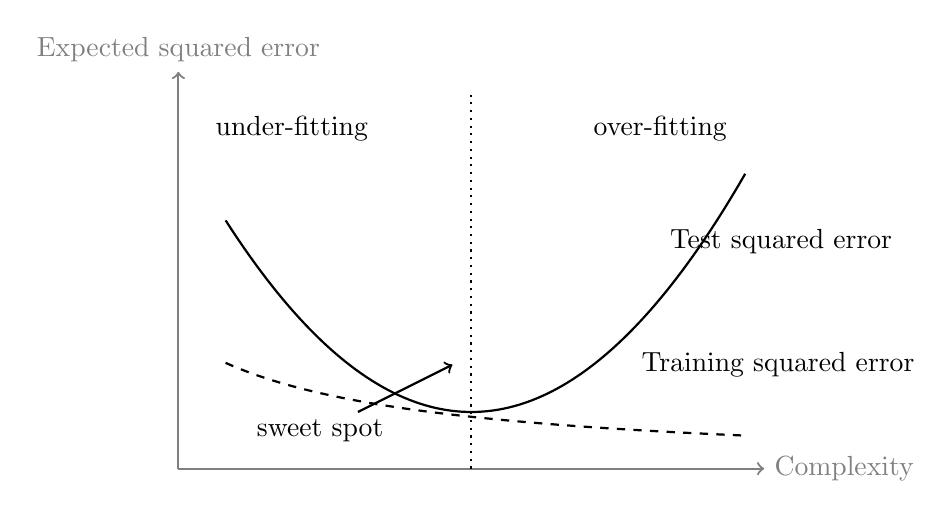
\begin{tikzpicture}[scale=1.2]
		% Axes
		\draw[->, thick, gray] (0,0) -- (6.2,0) node[right] {Complexity};
		\draw[->, thick, gray] (0,0) -- (0,4.2) node[above] {Expected squared error};
		
		% Labels for under-fitting and over-fitting
		\node at (1.2,3.6) {under-fitting};
		\node at (5.1,3.6) {over-fitting};
		
		% Training risk curve
		\draw[thick, dashed, domain=0.5:6, samples=100] plot(\x, {1.4/(0.5*\x + 1)});
		\node[right] at (4.8,1.1) {Training squared error};
		
		% Test risk curve
		\draw[thick, domain=0.5:6, samples=100] plot(\x, {0.3*(\x - 3.1)^2 + 0.6});
		\node[right] at (5.1,2.4) {Test squared error};
		
		% Sweet spot annotation
		\draw[->, thick] (1.9,0.6) -- (2.9,1.1);
		\node[align=center] at (1.5,0.4) {sweet spot};
		
		% Vertical line at optimal capacity
		\draw[dotted, thick] (3.1,0) -- (3.1,4);
		
	\end{tikzpicture}
\begin{tablenotes}
	\item \small{\textbf{Notes:} Curves for training squared error (dashed line) and test squared error (solid line). The classical U-shaped error curve arising from the bias–variance trade-off.}
\end{tablenotes}
\caption{\textit{Bias-variance trade-off} in machine learning.}
\label{fig:bias_var}
\end{figure}
    
To avoid overfitting in machine learning, an important step called \textit{cross-validation} is often employed. This involves splitting the dataset into multiple parts (called \textit{folds}) and systematically training and testing models on these parts \cite{hastie2009elements,efron2021computer}. The main goal is to evaluate how well models generalize to ``unseen data''.

There is a compelling justification for cross-validation within Bayesian inference proposed by \cite{Bernardo1994} in their section 6.1.6. The point of departure is to assume an $\mathcal{M}$-open view of nature, in which there exists a set of models $\mathcal{M} = \left\{M_j : j \in J\right\}$ under comparison, but none of them represents the true data-generating process, which is assumed to be unknown. Nevertheless, we can compare the models in $\mathcal{M}$ based on their posterior risk functions (see Chapter~\ref{chap1}) without requiring the specification of a true model. In this framework, we select the model that minimizes the posterior expected loss. Unfortunately, we cannot explicitly compute this posterior expected loss due to the lack of knowledge of the true posterior distribution under the $\mathcal{M}$-open assumption.\footnote{This is not the case under an $\mathcal{M}$-closed view of nature, where one of the candidate models is assumed to be the true data-generating process. In that setting, the posterior distribution becomes a mixture distribution with mixing probabilities given by the posterior model probabilities (see Chapter~\ref{chap10}).}

Given the expected loss conditional on model \( j \) for a predictive problem, where the action \( a \) is chosen to minimize the posterior expected loss:
\begin{align*}
	\mathbb{E}_{y_0}[L(Y_0,a) \mid M_j, \mathbf{y}] &= \int_{\mathcal{Y}_0} L(y_0, a \mid M_j, \mathbf{y}) \, \pi(y_0 \mid \mathbf{y}) \, dy_0,
\end{align*}
we note that there are \( N \) possible partitions of the dataset \( \mathbf{y} = \{y_1, y_2, \dots, y_N\} \) following a leave-one-out strategy, i.e., \( \mathbf{y} = \{\mathbf{y}_{-k}, y_k\} \), for \( k = 1, \dots, N \), where \( \mathbf{y}_{-k} \) denotes the dataset excluding observation \( y_k \). Assuming that \( \mathbf{y} \) is exchangeable, meaning its joint distribution is invariant to reordering, and that \( N \) is large, then \( \mathbf{y}_{-k} \) and \( y_k \) are good proxies for \( \mathbf{y} \) and \( y_0 \), respectively. Consequently,
\begin{align*}
	\frac{1}{K} \sum_{k=1}^K L(y_k, a \mid M_j, \mathbf{y}_{-k}) 
	\stackrel{p}{\rightarrow}\int_{\mathcal{Y}_0} L(y_0, a \mid M_j, \mathbf{y}) \, \pi(y_0 \mid \mathbf{y}) \, dy_0,
\end{align*}
by the law of large numbers, as \( N \to \infty \) and \( K \to \infty \).

Thus, we can select a model by minimizing the expected squared error based on its expected predictions \( \mathbb{E}[y_k \mid M_j, \mathbf{y}_{-k}] \); that is, we select the model with the lowest value of
\[
\frac{1}{K} \sum_{k=1}^K \left( \mathbb{E}[y_k \mid M_j, \mathbf{y}_{-k}] - y_k \right)^2.
\]

Note that if we want to compare two models based on their relative predictive accuracy using the log-score function \cite{martin2022optimal}, we select model \( j \) if
\begin{align*}
	\int_{\mathcal{Y}_0} \log\frac{p(y_0 \mid M_j, \mathbf{y})}{p(y_0 \mid M_l, \mathbf{y})} \, \pi(y_0 \mid \mathbf{y}) \, dy_0 > 0.
\end{align*}
However, we know that
\begin{align*}
	\frac{1}{K}\sum_{k=1}^K\log\frac{p(y_k \mid M_j, \mathbf{y}_{-k})}{p(y_k \mid M_l, \mathbf{y}_{-k})} 
	\stackrel{p}{\rightarrow} \int_{\mathcal{Y}_0} \log\frac{p(y_0 \mid M_j, \mathbf{y})}{p(y_0 \mid M_l, \mathbf{y})} \, \pi(y_0 \mid \mathbf{y}) \, dy_0,
\end{align*}
by the law of large numbers as \( N \to \infty \) and \( K \to \infty \).

This implies that we select model \( j \) over model \( l \) if
\begin{align*}
	\prod_{k=1}^K \left( \frac{p(y_k \mid M_j, \mathbf{y}_{-k})}{p(y_k \mid M_l, \mathbf{y}_{-k})} \right)^{1/K} 
	= \prod_{k=1}^K \left( B_{jl}(y_k, \mathbf{y}_{-k}) \right)^{1/K} > 1,
\end{align*}
where \( B_{jl}(y_k, \mathbf{y}_{-k}) \) is the Bayes factor comparing model \( j \) to model \( l \), based on the posterior \( \pi(\boldsymbol{\theta}_m \mid M_m, \mathbf{y}_{-k}) \) and the predictive \( \pi(y_k \mid \boldsymbol{\theta}_m) \), for \( m \in \{j, l\} \).

Thus, under the log-score function, cross-validation reduces to the geometric average of Bayes factors that evaluate predictive performance based on the leave-one-out samples \( \mathbf{y}_{-k} \).

\section{Regularization}\label{sec13_2}

In this century, the amount of available data continues to grow. This means we have access to more covariates for prediction, and we can also generate additional features to enhance the predictive power of our models. As a result, we often encounter \textit{wide} datasets, where the number of features may exceed the number of observations. Even in modest settings, we might have hundreds of features, and we can use them to identify which ones contribute to accurate predictions. However, we generally avoid using all features at once due to the risk of overfitting. Thus, we require a class of feature selection or \textit{regularization}.

In the Frequentist inferential framework, there has been extensive development of techniques aimed at regularization. These include methods such as Ridge regression \cite{hoerl1970ridge}, discrete subset selection techniques like best subset selection \cite{furnival1974regressions}, and forward and backward stepwise selection \cite{hastie2009elements}, as well as continuous subset selection methods such as the LASSO \cite{tibshirani1996regression}, the elastic net \cite{zou2005regularization}, and OSCAR \cite{bondell2008simultaneous}. 

It is important to note, however, that Ridge regression does not perform variable selection; rather, it shrinks coefficient estimates toward zero without setting them exactly to zero.

Ridge regression and the LASSO can be viewed as special cases of a more general class of estimators known as \textit{Bridge regression} \cite{fu1998penalized}, which also admits a Bayesian interpretation. Consider the following penalized least squares criterion in the linear regression setting:
\begin{align*}
	\hat{\boldsymbol{\beta}}^{\text{Bridge}} = \arg\min_{\boldsymbol{\beta}} \left\{ \sum_{i=1}^N \left( y_i - \beta_0 - \sum_{k=1}^K w_{ik} \beta_k \right)^2 + \lambda \sum_{k=1}^K |\beta_k|^q \right\}, \quad q \geq 0.
\end{align*}
Note that in variable selection problems, it is important to standardize the features to avoid issues caused by differences in scale, otherwise, variables with larger magnitudes will be penalized less and dominate the regularization path.

Interpreting \( |\beta_k|^q \) as proportional to the negative log-prior density of \( \beta_k \), the penalty shapes the contours of the prior distribution on the parameters. Specifically:
\begin{itemize}
	\item \( q = 0 \) corresponds to best subset selection, where the penalty counts the number of nonzero coefficients.
	\item \( q = 1 \) yields the LASSO, which corresponds to a Laplace (double-exponential) prior.
	\item \( q = 2 \) yields ridge regression, which corresponds to a Gaussian prior.  
	 
\end{itemize}

In this light, best subset selection, the LASSO, and ridge regression can be viewed as maximum a posteriori (MAP) estimators under different priors centered at zero \cite{Park2008}. However, they are not Bayes estimators in the strict sense, since Bayes estimators are typically defined as the posterior \textit{mean}. While ridge regression coincides with the posterior mean under a Gaussian prior \cite{Ishwaran2005}, the LASSO and best subset selection yield posterior modes.

This distinction is important because the Bayesian framework naturally incorporates regularization through the use of proper priors, which helps mitigate overfitting. Specifically, when proper shrinkage priors are used, the posterior balances data likelihood and prior information, thus controlling model complexity.

Furthermore, empirical Bayes methods can be employed to estimate the scale parameter of the prior covariance matrix for the regression coefficients, which in turn determines the regularization strength in ridge regression.

\subsection{Bayesian LASSO}\label{sec13_21}
Given the popularity of the LASSO as a variable selection technique, we present its Bayesian formulation in this subsection \cite{Park2008}. The Gibbs sampler for the Bayesian LASSO exploits the representation of the Laplace distribution as a scale mixture of normals. This leads to the following hierarchical representation of the model:
\begin{align*}
	\mathbf{y} \mid \beta_0, \boldsymbol{\beta}, \sigma^2, \mathbf{W} &\sim {N}(\beta_0 \mathbf{1} + \mathbf{W} \boldsymbol{\beta}, \sigma^2 \mathbf{I}_N), \\
	\boldsymbol{\beta} \mid \sigma^2, \tau_1^2, \dots, \tau_K^2 &\sim {N}(\mathbf{0}_K, \sigma^2 \mathbf{D}_{\tau}), \\
	\tau_1^2, \dots, \tau_K^2 &\sim \prod_{k=1}^K \frac{\lambda^2}{2} \exp\left\{ -\frac{\lambda^2}{2} \tau_k^2 \right\}, \\
	\sigma^2 &\sim \frac{1}{\sigma^2},
\end{align*}
where $	\mathbf{D}_{\tau} = \operatorname{diag}(\tau_1^2, \dots, \tau_K^2)$. 

After integrating out \( \tau_1^2, \dots, \tau_K^2 \), the conditional prior of \( \boldsymbol{\beta} \mid \sigma^2 \) is:
\begin{align*}
	\pi(\boldsymbol{\beta} \mid \sigma^2) &= \prod_{k=1}^K \frac{\lambda}{2 \sqrt{\sigma^2}} \exp\left\{ -\frac{\lambda}{\sqrt{\sigma^2}} |\beta_k| \right\},
\end{align*}
which implies that the log-prior is proportional to \( \lambda \sum_{k=1}^K |\beta_k| \), matching the penalty term in the LASSO optimization problem.

We assume that \( \beta_0 \) has a flat prior distribution. Since it is not of primary interest, and given that all regressors are standardized, \( \beta_0 \) corresponds to the overall mean of \( \mathbf{y} \) and can be integrated out.

The conditional posterior distributions for the Gibbs sampler are \cite{Park2008}:
\begin{align*}
	\boldsymbol{\beta} \mid \sigma^2, \tau_1^2, \dots, \tau_K^2, \mathbf{W}, \tilde{\mathbf{y}} &\sim {N}(\boldsymbol{\beta}_n, \sigma^2 \mathbf{B}_n), \\
	\sigma^2 \mid \boldsymbol{\beta}, \tau_1^2, \dots, \tau_K^2, \mathbf{W}, \tilde{\mathbf{y}} &\sim \text{Inverse-Gamma}(\alpha_n/2, \delta_n/2), \\
	\tau_k \mid \boldsymbol{\beta}, \sigma^2, \mathbf{W}, \tilde{\mathbf{y}} &\sim \text{Inverse-Gaussian}(\mu_{kn}, \lambda_n),
\end{align*}
where:
\begin{align*}
	\boldsymbol{\beta}_n &= \mathbf{B}_n \mathbf{W}^{\top} \tilde{\mathbf{y}}, \\
	\mathbf{B}_n &= \left( \mathbf{W}^{\top} \mathbf{W} + \mathbf{D}_{\tau}^{-1} \right)^{-1}, \\
	\alpha_n &= (N - 1) + K, \\
	\delta_n &= (\tilde{\mathbf{y}} - \mathbf{W} \boldsymbol{\beta})^{\top} (\tilde{\mathbf{y}} - \mathbf{W} \boldsymbol{\beta}) + \boldsymbol{\beta}^{\top} \mathbf{D}_{\tau}^{-1} \boldsymbol{\beta}, \\
	\mu_{kn} &= \sqrt{ \frac{ \lambda^2 \sigma^2 }{ \beta_k^2 } }, \\
	\lambda_n &= \lambda^2,
\end{align*}
and $\tilde{\mathbf{y}}$ is the centered response vector.

In this formulation, we can interpret \( \tau_k \) as local shrinkage parameters, while \( \lambda \) serves as a global shrinkage parameter. Higher values of \( \lambda \) imply stronger shrinkage toward zero. \cite{Park2008} propose two methods for specifying the value of the global shrinkage parameter: empirical Bayes estimation or a fully Bayesian hierarchical approach, in which \( \lambda^2 \) is assigned a Gamma prior.

We should acknowledge that the Bayesian LASSO is more computationally expensive than the Frequentist LASSO. However, it provides credible intervals for the parameters automatically. In contrast, obtaining standard errors in the Frequentist LASSO is more challenging, particularly for parameters estimated to be exactly zero \cite{kyung2010penalized}.\\

\textbf{Example: Simulation exercise of the Bayesian LASSO}

We simulate the process \( y_i = \beta_0 + \sum_{k=1}^{10} w_{ik} \beta_k + \mu_i \), where \( \beta_k \sim \mathcal{U}(-3, 3) \), \( \mu_i \sim \mathcal{N}(0, 1) \), and \( w_{ik} \sim \mathcal{N}(0, 1) \), $i=1,2,\dots,500$. Additionally, we generate 90 extra potential features from a standard normal distribution, which are included in the model specification. Our goal is to assess whether the Bayesian LASSO can successfully identify the truly relevant features.

We use the \textit{bayesreg} package in \textbf{R} to perform the Bayesian LASSO, using 5,000 MCMC draws and 1,000 burn-in iterations. The following code illustrates the simulation exercise and compares the posterior means with the true population values.

The summary of the fit and the plot comparing the population parameters with the posterior means show that the Bayesian LASSO is able to identify the variables that are relevant in the data generating process. In Exercise 1, we propose programming the Gibbs sampler from scratch, assuming a hierarchical structure for the global shrinkage parameter, and comparing the results with those obtained using the \textit{monomvn} package.

\begin{tcolorbox}[enhanced,width=4.67in,center upper,
	fontupper=\large\bfseries,drop shadow southwest,sharp corners]
	\textit{R code. The Bayesian LASSO}
	\begin{VF}
		\begin{lstlisting}[language=R]
rm(list = ls()); set.seed(10101)
library(bayesreg)
# Parameters
n <- 500  # sample size
p <- 100  # number of predictors
s <- 10   # number of non-zero coefficients
# Generate design matrix
X <- matrix(rnorm(n * p), nrow = n, ncol = p)
# True beta: first s coefficients are non-zero, rest are zero
beta_true <- c(runif(s, -3, 3), rep(0, p - s))
# Generate response with some noise
sigma <- 1
y <- X %*% beta_true + rnorm(n, sd = sigma)
df <- data.frame(X,y)
### Using bayesreg ###
# Fit the model
fit <- bayesreg::bayesreg(y ~ X, data = df, model = "gaussian", prior = "lasso", 
n.samples = 5000, burnin = 1000)
# Check summary
summary(fit)
# Extract posterior means of beta
beta_post_mean <- rowMeans(fit$beta)
# Compare true vs estimated
plot(beta_true, beta_post_mean, pch = 19, col = "steelblue",
xlab = "True beta", ylab = "Posterior mean of beta",
main = "Bayesian LASSO Shrinkage")
abline(0, 1, col = "red", lty = 2)
\end{lstlisting}
	\end{VF}
\end{tcolorbox}
  
\subsection{Stochastic search variable selection}\label{sec13_22}

\subsection{Non-local priors}\label{sec13_23}

\cite{johnson2012bayesian}
R package: mombf (Model Selection with Bayesian Methods and Information Criteria)
link: https://cran.r-project.org/web/packages/mombf/index.html

\section{Bayesian additive regression trees}\label{sec13_3}

\section{Gaussian processes}\label{13_4}

Remember the relevance of GP in Bayesian optimization, and consequently, in pseudo-marginal MCMC, which is a case where the likelihood function cannot be evaluated exactly but can be estimated unbiasedly. This method is particularly useful in scenarios where latent variables or complex models make direct likelihood computations intractable.

\section{Large data problems}\label{13_5}
Review \cite{bardenet2017markov}
\begin{itemize}
	\item Subsampling MCMC: Firefly Monte Carlo \cite{Maclaurin2015}
	\item Stochastic Gradient MCMC (SG-MCMC): Stochastic Gradient Langevin Dynamics (SGLD) and Stochastic Gradient Hamiltonian Monte Carlo (SGHMC). See \cite{nemeth2021stochastic,song2020extended,baker2019sgmcmc,chen2014stochastic,welling2011bayesian}
	\item Divide-and-Conquer MCMC \cite{quiroz2018subsampling,quiroz2019speeding}: Consensus Monte Carlo \cite{rendell2020global,scott2022bayes} and Weierstrass Sampler \cite{wu2017average}
\end{itemize}

\begin{tcolorbox}[enhanced,width=4.67in,center upper,
	fontupper=\large\bfseries,drop shadow southwest,sharp corners]
	\textit{R code. Stochastic Gradient MCMC (SG-MCMC): Linear regression}
	\begin{VF}
		\begin{lstlisting}[language=R]
set.seed(123)

# Simulated data
n <- 10000  # Large n for SGLD to shine
p <- 3
X <- cbind(1, matrix(rnorm(n * (p - 1)), n, p - 1))  # design matrix
beta_true <- c(1, -2, 0.5)
sigma2 <- 1
y <- X %*% beta_true + rnorm(n, 0, sqrt(sigma2))

# SGLD settings
iterations <- 2000
batch_size <- 100
stepsize <- 1e-4
beta <- rep(0, p)  # initial value
trace_beta <- matrix(NA, nrow = iterations, ncol = p)

# Log posterior gradient function (Gaussian likelihood and prior)
grad_log_post <- function(beta, X_batch, y_batch, n, sigma2) {
	p <- length(beta)
	grad_loglik <- t(X_batch) %*% (y_batch - X_batch %*% beta) / sigma2
	grad_logprior <- -beta  # derivative of log N(0, I)
	return((n / nrow(X_batch)) * grad_loglik + grad_logprior)
}

# SGLD algorithm
for (t in 1:iterations) {
	idx <- sample(1:n, batch_size)
	X_batch <- X[idx, ]
	y_batch <- y[idx]
	
	grad <- grad_log_post(beta, X_batch, y_batch, n, sigma2)
	noise <- rnorm(p, 0, sqrt(stepsize))
	beta <- beta + 0.5 * stepsize * grad + noise
	trace_beta[t, ] <- beta
}

# Plot evolution of beta[2] (can change to others)
plot(trace_beta[, 2], type = "l", col = "blue", lwd = 2,
main = expression("SGLD: Evolution of " * beta[2]),
xlab = "Iteration", ylab = expression(beta[2]))
abline(h = beta_true[2], col = "red", lty = 2)
legend("bottomright", legend = c("SGLD", "True value"),
col = c("blue", "red"), lty = c(1, 2))
		\end{lstlisting}
	\end{VF}
\end{tcolorbox}

\section{Summary}\label{13_6}
Variational Bayes, a method rooted in machine learning \cite{wainwright2008graphical}, is introduced in Chapter \ref{chap15}. When implemented in its stochastic form, it can effectively address the tall problem.

\section{Exercises}\label{13_7}

\begin{enumerate}
	\item \textbf{Simulation exercise: the Bayesian LASSO continues}
	
	Program the Gibbs sampler for the Bayesian LASSO from scratch, assuming a hierarchical structure for the global shrinkage parameter. Perform inference using this sampler in the Bayesian LASSO simulation exercise. Compare the results with those obtained using the \textit{monomvn} package.

\end{enumerate}


\chapter{Spatial econometric models}\label{chap14}
\chapter{Approximate Bayesian methods}\label{chap15}

\textit{Approximate Bayesian methods} are a family of techniques designed to handle situations where the likelihood function lacks an analytical expression, is highly complex, or the problem has high dimensionality, whether due to a large parameter space or a massive dataset \cite{martin2024approximating}. In the former case, traditional Markov Chain Monte Carlo (MCMC) and importance sampling algorithms fail to provide a solution, while in the latter, these algorithms struggle to produce accurate estimates within a reasonable time.  

However, there is no free lunch, \textit{Approximate Bayesian methods} address these challenges at the cost of providing an approximation to the posterior distribution rather than the \textit{exact} posterior. Nonetheless, asymptotic results show that the approximation improves as the sample size increases.

In this chapter, I first present \textit{simulation-based approaches}, which are designed to address situations where the likelihood is highly complex and may lack an analytical solution. In the second part, I introduce \textit{optimization approaches}, which are intended to handle high-dimensional problems. Specifically, I discuss approximate Bayesian computation (ABC) and Bayesian synthetic likelihood (BSL), the two most common \textit{simulation-based approaches}. Then, I present integrated nested Laplace approximations (INLA) and \textit{variational Bayes} (VB), the two most common \textit{optimization approaches} for high-dimensional problems.

\section{Simulation-based approaches}\label{sec15_1}
Taking into account the fundamental equation for performing parameter inference in the Bayesian framework,  
\begin{align*}
	\pi(\boldsymbol{\theta} \mid \mathbf{y}) & \propto p(\mathbf{y} \mid \boldsymbol{\theta}) \times \pi(\boldsymbol{\theta}),
\end{align*}  
we see in Section \ref{sec51} that MCMC algorithms, such as the Gibbs sampler (Section \ref{sec511}) and Metropolis-Hastings (Section \ref{sec512}), require evaluation of the likelihood function \( p(\boldsymbol{y} \mid \boldsymbol{\theta}) \) in the posterior conditional distribution or the acceptance probability, respectively. This is also the case for importance sampling when calculating the importance weights (Section \ref{sec52}).  

Thus, what happens when the likelihood function does not have an analytical expression? This situation arises in many models involving unobserved heterogeneity (i.e., unobserved taste preferences), models defined by quantile functions (e.g., the g-and-k distribution), or dynamic equilibrium model (e.g., repeated game models).

\textit{Simulation-based algorithms} provide a Bayesian solution when we face this situation, namely, when the likelihood function lacks an analytical expression or is highly complex. The only requirement is that we must be able to simulate synthetic data from the model conditional on the parameters. Therefore, these algorithms obtain an approximation to the posterior draws by simulating from the prior distribution $\pi(\boldsymbol{\theta})$ and then using these draws to simulate from the likelihood $p(\mathbf{y} \mid \boldsymbol{\theta})$.

\subsection{Approximate Bayesian computation}\label{sec15_12}

\textit{Approximate Bayesian Computation} (ABC) is designed to handle inferential situations where the likelihood function \( p(\boldsymbol{y} \mid \boldsymbol{\theta}) \) is intractable or highly complex. It was introduced in population genetics by \cite{tavare1997inferring, pritchard1999population} and later generalized by \cite{beaumont2002approximate}. The basic intuitive origin of ABC appears to have been introduced by \cite{rubin1984bayesianly}. A growing body of literature explores its applications in biology, cosmology, finance, economics, and other fields.

The requirement in ABC is the ability to simulate from the parametric model. The process begins by drawing samples from the prior distribution \( \pi({\boldsymbol{\theta}}) \) multiple times, $\boldsymbol{\theta}\in\mathbb{R}^K$, and then simulating data from the model given each \( {\boldsymbol{\theta}^{(s)}}, s=1,2,\dots,S \). The resulting synthetic data, \( \boldsymbol{z}^{(s)} \in \mathbb{R}^n \) is used to compute summary statistics \( \boldsymbol{\eta}(\boldsymbol{z}^{(s)}) \in \mathbb{R}^L, L\geq K \). These summary statistics are crucial for the performance of ABC and should be selected based on a thorough understanding of the model.  

Next, we compare the synthetic summary statistics with the observed summary statistics \( \boldsymbol{\eta}(\boldsymbol{y}) \) using a distance metric \( d\left\{ \boldsymbol\eta ({\boldsymbol y}),{\boldsymbol \eta }({\boldsymbol z}^{(s)})\right\} \), typically the Euclidean distance. We retain the prior draws that generate synthetic summary statistics closest to the observed ones, that is, \( d\left\{ \boldsymbol\eta ({\boldsymbol y}),{\boldsymbol \eta }({\boldsymbol z}^{(s)})\right\}\leq \epsilon \), forming an approximation of the posterior distribution \( \pi_{\epsilon}(\boldsymbol{\theta},\boldsymbol{z} \mid \boldsymbol{\eta}(\boldsymbol{y})) \).

The simplest algorithm is the accept/reject approximate Bayesian computation (ABC-AR) (see Algorithm \ref{ABC0}).

\begin{algorithm}
	\caption{Accept/reject ABC}\label{ABC0}
	\begin{algorithmic}[1]
		\For{\texttt{$s=1,\dots,S$}}
		\State Draw ${\boldsymbol {\theta} }^{s}$ from $\pi({ \boldsymbol{\theta} }),$
		\State Simulate ${\boldsymbol z}^{s}=(z_{1}^{s},z_{2}^{s},...,z_{n}^{s})^{\top}$from the model, $p(\cdot|{\boldsymbol{\theta} }^{s})$
		\State Calculate
		$d_{(s)}=d\{{\boldsymbol\eta }({\boldsymbol y}),{\boldsymbol \eta }({\boldsymbol z}^{s})\}$
		\EndFor
		\State Order the distances $d_{(1)}\leq\cdots\leq d_{(S)}$
		\State Select all $\boldsymbol{\theta}^s$ such that $d_{(i)}\leq \epsilon$, where $\epsilon>0$ is the tolerance level. 
	\end{algorithmic}
\end{algorithm}

Note that the posterior distribution is conditional on the summary statistics \( \boldsymbol{\eta}(\boldsymbol{y}) \) and the tolerance parameter \( \epsilon \). This implies that we obtain an approximation to the target distribution \( \pi(\boldsymbol{\theta} \mid \boldsymbol{y}) \) because \( \boldsymbol{\eta}(\boldsymbol{y}) \) is not a sufficient statistic in most cases, and \( \epsilon > 0 \), these conditions introduce bias \cite{blum2010approximate}. However, ABC performs well compared to full-likelihood approaches in low-dimensional parameter spaces \cite{beaumont2002approximate}.

Furthermore, \cite{frazier2018asymptotic} show in Theorems 1 and 2 that Bayesian consistency and asymptotic normality hold, provided that \( \epsilon \to 0 \) fast enough as \( n \to +\infty \). In particular, the requirement is that the proportion of accepted draws converges to 0 at a rate of \( n^{-K / 2} \). Additionally, Theorem 2 in \cite{frazier2018asymptotic} shows that \( 100(1 -\alpha)\% \) Bayesian credible regions using ABC have frequentist coverage of \( 100(1 -\alpha)\% \). 

We should note from these asymptotic results that ABC suffers from the \textit{curse of dimensionality}. Specifically, given a sample size of 1,000 and two parameters, the proportion of accepted draws should be 0.1\%, meaning we would require one million prior draws to obtain 1,000 posterior draws. On the other hand, if the number of parameters is three, we would require 31.62 million prior draws. This limitation of ABC has attracted attention; see Chapter 8 of \cite{sisson2018handbook} for some potential solutions.

It is a common practice in ABC to perform a regression adjustment after retaining the draws \cite{beaumont2002approximate, leuenberger2010bayesian, sisson2018handbook}. This adjustment reduces bias in posterior draws by performing a simple linear regression between the selected draws and the discrepancy between the observed and simulated summary statistics, \( {\theta}^{(s)}_k = \alpha + \left(\boldsymbol{\eta}(\boldsymbol{y}) - \boldsymbol{\eta}(\boldsymbol{z}^{(s)})\right)^{\top}\boldsymbol{\beta} + \mu^{(s)}, \ k=1,2,\dots,K \). Then, the posterior draws are adjusted using the slope estimate \( {\theta}^{\text{adj},(s)}_k = {\theta}^{(s)} - \left(\boldsymbol{\eta}(\boldsymbol{y}) - \boldsymbol{\eta}(\boldsymbol{z}^{(s)})\right)^{\top}\hat{\boldsymbol{\beta}} \). Other regression adjustment strategies are also used, such as local linear regression, ridge regression, and neural networks. See the \textit{abc} package in \textbf{R}.

The favorable asymptotic sampling properties of ABC rely on correct model specification. However, \cite{frazier2020model} demonstrate that when the assumed model is misspecified, the asymptotic behavior of ABC can deteriorate. In particular, the posterior shape becomes asymptotically non-Gaussian, and the behavior of the posterior mean remains generally unknown. Additionally, regression adjustment approaches can produce posteriors that differ significantly from their simpler accept/reject counterparts.

Given these concerns, testing model specification in ABC is essential. This can be done using simulated goodness-of-fit statistics \cite{bertorelle2010abc,lintusaari2017fundamentals}, predictive p-values \cite{bertorelle2010abc}, discrepancy diagnostics \cite{frazier2020model}, and asymptotic tests \cite{ramirez2024testing} to evaluate model adequacy.

The accept/reject ABC algorithm is inefficient, as all draws are independent; thus, there is no learning from previous draws. This intensifies the computational burden. Therefore, \cite{marjoram2003markov, wegmann2009efficient} introduced Markov Chain Monte Carlo ABC (ABC-MCMC) algorithms, and \cite{sisson2007sequential, drovandi2011estimation, del2012adaptive, lenormand2013adaptive} proposed sequential Monte Carlo approaches (ABC-SMC). However, results comparing ABC-MCMC and ABC-SMC with ABC-AR are controversial regarding computational efficiency \cite{bertorelle2010abc}. In addition, ABC-AR is very simple and easily allows parallel computing \cite{frazier2019approximate}. Nevertheless, ABC-SMC is now the recommended approach, as it does not require tuning the algorithm's tolerance \cite{martin2024approximating}, and there are open-source implementations that facilitate its use.

New developments in ABC have focused on using empirical measures calculated from the observed ($\hat{\mu}_n$) and synthetic ($\hat{\mu}_{\boldsymbol{\theta}}^{(s)}$) data to replace summary statistics. Thus, $d\left\{ \boldsymbol\eta ({\boldsymbol y}),{\boldsymbol \eta }({\boldsymbol z}^{(s)})\right\}$ is replaced by $\mathcal{D}\left\{ \hat{\mu}_n,\hat{\mu}_{\boldsymbol{\theta}}^{(s)}\right\}$, where the latter is a discrepancy measure, such as the Kullback-Leibler divergence \cite{jiang2018approximate}. However, \cite{drovandi2022comparison} found in their simulation exercises that the best-performing summary statistics approach performs at least as well as the best discrepancy-measure approaches. The key point is to select informative summary statistics.\\

\textbf{Example: g-and-k distribution for financial returns} 

The g-and-k distribution is a highly flexible distribution capable of capturing skewness and heavy tails through its parameters. This makes it particularly useful for modeling real-world data that deviate from normality, especially in fields like finance, where outliers are common. However, this distribution lacks a closed-form expression for its density function.

The g-and-k distribution is defined by its quantile function \cite{drovandi2011likelihood}. Specifically, it is specified through its inverse cumulative distribution function,

\[
Q(p\mid{\theta}) = F^{-1}(p\mid{\theta}),
\]

where \( F = P(U \leq u) \), and \( Q \) represents the \( p \)-quantile \cite{rayner2002numerical}. The quantile function of the g-and-k distribution is given by

\[
Q^{gk}\left\{z(p)\mid a, b, c, g, k\right\} = a + b\left[1 + c \frac{1 - \exp\left\{-gz(p)\right\}}{1 + \exp\left\{-gz(p)\right\}}\right] \left\{1 + z(p)^2\right\}^k z(p),
\]

where \( z(p) \) is the standard normal quantile function, and \( c = 0.8 \) is a commonly suggested value.

In the g-and-k distribution, \( a \) is the location parameter, and \( b \) is the scale parameter, controlling the dispersion. The parameters \( g \) and \( k \) determine the levels of skewness and kurtosis, respectively, while \( c \) modifies the impact of skewness, and is typically set to 0.8.

\cite{drovandi2011likelihood} propose a moving average of order one using a g-and-k distribution to model exchange rate log returns. In particular,  
\[
z_t = \epsilon_t + \theta_1\epsilon_{t-1}, \quad t=1,\dots,524,
\]  
where \(\epsilon_t \sim N(0,1)\).  

The values of \(z_t\) are then divided by \((1+\theta_1^2)^{1/2}\) to ensure that they marginally follow a standard normal distribution. Thus, simulating g-and-k data requires only substituting \(z_t\) into the quantile function.  

We model exchange rate log daily returns from USD/EUR one year before and after the WHO declared the COVID-19 pandemic on 11 March 2020. We use the dataset \textit{ExchangeRate.csv} from our GitHub repository. Our ABC implementation uses twelve summary statistics: the seven octiles, the interquartile range, robust measures of skewness and kurtosis, and the autocorrelations of order one and two (see \cite{drovandi2011likelihood} and code below). We adopt the prior distributions proposed by \cite{ramirez2024testing}, 
\begin{align*}
	\theta_1\sim U(-1,1), \ a\sim U(0,5) \ b\sim U(0,5)\\
	g\sim U(-5,5), \ k\sim U(-0.5, 5).
\end{align*}

We use the \textit{EasyABC} package in \textbf{R} to implement the ABC accept/reject (ABC-AR) algorithm using 150,000 prior draws with an acceptance rate of 0.67\%. We also apply the ABC Markov chain Monte Carlo (ABC-MCMC) method \cite{marjoram2003markov} and the sequential Monte Carlo ABC (ABC-SMC) method \cite{lenormand2013adaptive} to compare the results across different ABC algorithms.\footnote{Note that this setting does not satisfy the asymptotic requirements for Bayesian consistency. However, it serves as a pedagogical exercise.} We generate 100,000 samples and retain 1\% in ABC-MCMC, and 30,000 samples, keeping 3.4\%, with a stopping criterion of 5\% in ABC-SMC. These settings imply that the three algorithms require approximately the same computational time. Users can refer to the cited references for algorithmic details.

In Exercise 1, we ask to program the ABC accept/reject algorithm (Algorithm \ref{ABC0}) from scratch and compare the results with those obtained using the ABC-AR implementation in the \textit{EasyABC} package.

The following code presents the results, and Figure \ref{figABCexc} compares the posterior distributions of $\theta_1$, $g$, and $k$ using the three methods. In this figure, we observe that ABC-MCMC (red) and ABC-SMC (green) exhibit similar performance, and both approaches provide more information than ABC-AR (blue). There is marginal positive evidence that the moving average coefficient is positive, and the three algorithms yield similar means, although ABC-AR exhibits lower precision. Since the posterior distribution of $g$ is centered around zero, the distribution appears to be symmetric around its median. Meanwhile, a positive $k$ indicates that the distribution has heavier tails than a normal distribution, implying a higher likelihood of extreme values (outliers) in the exchange rate USD/EURO.

\begin{tcolorbox}[enhanced,width=4.67in,center upper,
	fontupper=\large\bfseries,drop shadow southwest,sharp corners]
	\textit{R code. Exchange rate log returns: Approximate Bayesian computation}
	\begin{VF}
		\begin{lstlisting}[language=R]
######### ABC Exchange rate og returns: USD/EURO
rm(list = ls()); set.seed(010101)
library(EasyABC)
dfExcRate <- read.csv(file = "https://raw.githubusercontent.com/BEsmarter-consultancy/BSTApp/refs/heads/master/DataApp/ExchangeRate.csv", sep = ",", header = T)
attach(dfExcRate); n <- length(USDEUR)
# Summary statistics
SumSt <- function(y) {
	Oct <- quantile(y, c(0.125, 0.25, 0.375, 0.5, 0.625, 0.75, 0.875))
	eta1 <- Oct[6] - Oct[2]
	eta2 <- (Oct[6] + Oct[2] - 2 * Oct[4]) / eta1
	eta3 <- (Oct[7] - Oct[5] + Oct[3] - Oct[1]) / eta1
	autocor <- acf(y, lag = 2, plot = FALSE)
	autocor[["acf"]][2:3]
	Etay <- c(Oct, eta1, eta2, eta3, autocor[["acf"]][2:3])
	return(Etay)
}
# g-and-k distribution
RGKnewSum <- function(par) {
	z <- NULL
	theta <- par[1]; a <- par[2]; b <- par[3]; g <- par[4]; k <- par[5]
	e <- rnorm(n + 1)
	for(t in 2:(n + 1)){
		zt <- e[t] + theta * e[t-1]
		z <- c(z, zt)
	}
	zs <- z / (1 + theta^2)^0.5
	x <- a + b * (1 + 0.8 * (1 - exp(-g * zs)) / (1 + exp(-g * zs))) * (1 + zs^2)^k * zs
	Etaz <- SumSt(x)
	return(Etaz)
}
toy_prior <- list(c("unif",-1,1), c("unif",0,5), c("unif", 0,5), c("unif", -5,5), c("unif", -0.5,5))
sum_stat_obs <- SumSt(USDEUR)
tick <- Sys.time()
ABC_AR <- ABC_rejection(model=RGKnewSum, prior=toy_prior, summary_stat_target = sum_stat_obs, nb_simul=150000, tol = 0.0067,
progress_bar = TRUE)
tock <- Sys.time()
tock - tick
PostABCAR <- coda::mcmc(ABC_AR$param)
summary(PostABCAR)
tick <- Sys.time()
ABC_MCMC <- ABC_mcmc(method="Marjoram", model=RGKnewSum, prior=toy_prior, summary_stat_target=sum_stat_obs, n_rec = 100000, progress_bar = TRUE)
tock <- Sys.time()
tock - tick
PostABCMCMC <- coda::mcmc(ABC_MCMC[["param"]][order(ABC_MCMC[["dist"]])[1:1000],])
summary(PostABCMCMC)
tick <- Sys.time()
\end{lstlisting}
	\end{VF}
\end{tcolorbox}

\begin{tcolorbox}[enhanced,width=4.67in,center upper,
	fontupper=\large\bfseries,drop shadow southwest,sharp corners]
	\textit{R code. Exchange rate log returns: Approximate Bayesian computation}
	\begin{VF}
		\begin{lstlisting}[language=R]
ABC_SMC<-ABC_sequential(method="Lenormand", model=RGKnewSum, prior=toy_prior, summary_stat_target=sum_stat_obs, nb_simul = 30000, alpha = 0.034, p_acc_min = 0.05,
progress_bar = TRUE)
summary(PostABCSMC)
tock <- Sys.time()
tock - tick
PostABCSMC <- coda::mcmc(ABC_SMC[["param"]])
		\end{lstlisting}
	\end{VF}
\end{tcolorbox}

\begin{figure}[!h]
	\includegraphics[width=340pt, height=200pt]{Chapters/chapter15/figures/ABCexcrate.png}
	\caption[List of figure caption goes here]{Approximate Bayesian computation: Exchange rate log returns USD/EURO.}\label{figABCexc}
\end{figure}

\subsection{Bayesian synthetic likelihood}\label{sec15_13}

Note that in ABC in most cases we are targeting the posterior distribution $\pi(\boldsymbol{\theta}\mid \boldsymbol{\eta}(\boldsymbol{y}))$ rather than $\pi(\boldsymbol{\theta}\mid \boldsymbol{y})$ as $\boldsymbol{\eta}(\boldsymbol{y})$ is not a sufficient statistic. This can be good as discarding information can improve the behaviour of the likelihood or make the inference more robust to misspecification \cite{price2018bayesian}.  

In Bayesian synthetic likelihood (BSL) adopts a Gaussian parametric approximation to 

\section{Optimization approaches}\label{sec15_2}

Even in situations where the likelihood function has an analytical expression, but there are huge datasets, MCMC and IS algorithms require pointwise evaluation of the likelihood function. This implies a huge number of operations, and these methods are not designed to be \textit{scalable}. Further, if there is a large parameter space, these methods are neither \textit{scalable} in the number of parameters.

\textit{Optimization approaches} are designed to scale to high parameter spaces and large datasets. The trick is to change simulation with optimization. 

\subsection{Integrated nested Laplace approximations}\label{sec15_21}
\textit{Integrated nested Laplace approximations} approximates $\pi(\boldsymbol{\theta} \mid \mathbf{y})$ by a combination of low-dimensional deterministic integration and optimization steps. 

\subsection{Variational Bayes}\label{sec15_22}
\textit{Variational Bayes} replaces $\pi(\boldsymbol{\theta} \mid \mathbf{y})$ by an approximation produced by calculus of variations. 

\section{Summary}\label{sec15_3}
\textit{Simulation-based algorithms} suffer from the \textit{curse of dimensionality} in parameter space, whereas \textit{Optimization approaches} require evaluation of the likelihood functions. Thus, recent approaches mix these two approaches to overcome situations where both phenomena are present.

\section{Exercises}\label{sec15_4}

\begin{enumerate}
	\item \textbf{g-and-k distribution for financial returns continues}
	
	Simulate a dataset following the specification given in the g-and-k distribution for financial returns example. Set $\theta_1 = 0.8$, $a = 1$, $b = 0.5$, $g = -1$, and $k = 1$, with a sample size of 500, and use the same prior as in this example. Implement the ABC accept/reject algorithm from scratch using one million prior draws, selecting the 1,000 draws with the smallest distance.\footnote{Note that this setting does not satisfy the asymptotic requirements for Bayesian consistency. However, it serves as a pedagogical exercise.}
	
	\begin{itemize}
		\item Perform a linear regression adjustment using the posterior draws of our ABC-AR algorithm (ABC-AR-Adj).
		\item Compare the results with those obtained using the ABC-AR implementation in the \textit{EasyABC} package, ensuring that the computational time is relatively similar between both implementations.
		\item Compare the posterior results of ABC-AR, ABC-AR-Adj and EasyABC with the population values.
	\end{itemize}
	
	\begin{comment}
	\item Simulate a model $y_i=0.5 x_i+u_i, \ i=1,2,\dots,250$, where 
	
	$$v_i=Q^{gk}\left\{z(p)\mid a_i, b_j, c_j, g_j, k_j\right\}, \  v_j=(x_j,u_j), \ \begin{Bmatrix} z(p_x) \\ z(p_u)\end{Bmatrix}\sim N \begin{Bmatrix} \begin{pmatrix} 0\\ 0\end{pmatrix}, \begin{pmatrix} 1 & 0.5 \\ 0.5 & 1\end{pmatrix} \end{Bmatrix}.$$
	
	Note that in this model there endogeneity as $x_j$ and the stochastic errors ($u_j$) are no independent.
	
	We took into account values for $\rho =\left\{0,0.4,0.8\right\}$, $\rho\neq 0$ implies that inference should be based on the joint likelihood function, $y_{j}=0.5x_j+u_j$ where $a_x=a_u=0$, $b_x=b_u=1$, $c_x=c_u=0.8$, $g_x=g_u=2$, $k_x=k_u=1$, and $n=(500, 1000)$ in 50 simulation exercises. We perform inference regarding $\beta$ and $k$ in this example, and fixed $a, b$ and $g$ at their population values. We consider as the basis of our analysis the summary statistics $\eta_{1}({y})=\sum_{i=1}^{n}x_iy_i/\sum_{i=1}^{n}x_i^2$, $\eta_2({y})=L_3-L_1$, $\eta_3({y})=(L_3+L_1-2L_2)/\eta_2$  and $\eta_4({y})=(E_7-E_5+E_3-E_1)/\eta_2$ where $L_l$ is the $l$th quartile and $E_l$ is the $l$th octile of $y_j-x_j\eta_1({y})$ \cite{drovandi2011likelihood}.
	\end{comment}

\item 
	
\end{enumerate}



\bibliographystyle{plain}
\bibliography{bibtex_example}

\printindex

\end{document}
